\documentclass[12pt,a4paper]{article}
% Science Monk -- NEET Physics book: page design and question macros
\usepackage[a4paper,top=1.75cm,bottom=1.6cm,left=1.35cm,right=1.35cm,
            headheight=14pt,headsep=0.3cm,footskip=0.65cm,columnsep=0.6cm]{geometry}
\usepackage[T1]{fontenc}
\usepackage[lining]{baskervillef}
\usepackage[baskervillef,vvarbb,upint]{newtxmath}
\usepackage[scaled=0.95]{inconsolata}
\usepackage{microtype}
\usepackage{miama}
\usepackage{calligra}
\usepackage{amsmath}
\usepackage{xcolor}
\usepackage{graphicx}
\usepackage{multicol}
\usepackage{enumitem}
\usepackage{array,tabularx,booktabs}
\usepackage{tikz}
\usetikzlibrary{arrows.meta,calc,patterns,decorations.pathmorphing,
                decorations.markings,decorations.pathreplacing,shapes.geometric,
                positioning,intersections,angles,quotes}
\usepackage[american]{circuitikz}
\ctikzset{bipoles/length=0.9cm}
\usepackage{pgfornament}
\usepackage{eso-pic}
\usepackage{fancyhdr}
\usepackage{titlesec}
\usepackage{needspace}
\usepackage[export]{adjustbox}
\usepackage{etoolbox}
\usepackage{pgfplots}
\pgfplotsset{compat=1.18}
\usepackage[hidelinks,bookmarksnumbered]{hyperref}
\usepackage{xurl}

% ---------- Palette: British navy, Italian green, French crimson, gilt ------
% Royal palette: burgundy, antique gold, bottle green on warm ivory (matches the logo's saffron/gold)
\definecolor{parchment}{HTML}{FFFEFB}  % near-white page
\definecolor{navy}{HTML}{6B1E2A}      % primary: royal burgundy (name kept for macros)
\definecolor{crimson}{HTML}{8A5A12}   % accent: deep saffron-bronze
\definecolor{verde}{HTML}{2F5D46}     % bottle green
\definecolor{gilt}{HTML}{B38B3C}      % antique gold
\definecolor{ink}{HTML}{2A1E18}       % sepia-black text
\definecolor{softgilt}{HTML}{E8D9B5}
\definecolor{ivory}{HTML}{FFFEFA}
\pagecolor{parchment}
\color{ink}

% ---------- Page frame: one thin gilt rule close to the page edge ---------
\newcommand{\pageframe}{%
  \begin{tikzpicture}[remember picture,overlay]
    \draw[gilt!80,line width=0.5pt] ($(current page.south west)+(0.6cm,0.6cm)$) rectangle ($(current page.north east)+(-0.6cm,-0.6cm)$);
  \end{tikzpicture}}
\newif\ifwatermark \watermarktrue
\newcommand{\watermarklogo}{\ifwatermark
  \begin{tikzpicture}[remember picture,overlay]
    \node[opacity=0.045,inner sep=0pt] at ($(current page.center)+(0,-0.3cm)$)
      {
\includegraphics[width=12.5cm]{img/logo}};
  \end{tikzpicture}\fi}
\AddToShipoutPictureBG{\watermarklogo\pageframe}

% ---------- Running heads -------------------------------------------------
\newcommand{\curyear}{}
\pagestyle{fancy}
\fancyhf{}
\renewcommand{\headrulewidth}{0pt}
\fancyhead[L]{\small\color{navy}\textsc{Science Monk}}
\fancyhead[R]{\small\color{crimson}\textit{NEET Physics \curyear}}
\fancyfoot[C]{\small\color{navy}\textendash~\thepage~\textendash}
\fancypagestyle{plain}{\fancyhf{}\fancyfoot[C]{\small\color{navy}\textendash~\thepage~\textendash}}

% ---------- Year chapter opener --------------------------------------------
\newcounter{qno}
\newcommand{\yearpaper}[3]{% #1 year, #2 exam date / set line, #3 note
  \clearpage
  \renewcommand{\curyear}{#1}%
  \setcounter{qno}{0}%
  \phantomsection\addcontentsline{toc}{section}{NEET #1 Physics}\label{p#1}%
  \begin{center}
    {\pgfornament[width=5cm,color=gilt]{87}}\par\vspace{2pt}
    {\fontsize{24}{28}\selectfont\color{navy}\scshape NEET #1}\par\vspace{2pt}
    {\Large\color{crimson}\itshape Physics Question Paper}\par\vspace{4pt}
    {\small #2}\par
    \ifstrempty{#3}{}{\vspace{2pt}{\footnotesize\itshape #3}\par}
    \vspace{3pt}{\pgfornament[width=5cm,color=gilt,symmetry=h]{87}}
  \end{center}
  \vspace{2pt}}

% ---------- Questions ---------------------------------------------------------
\setlength{\parindent}{0pt}
\setlength{\columnseprule}{0.4pt}
\renewcommand{\columnseprulecolor}{\color{gilt!60}}
\raggedcolumns
\newlength{\optw}\newlength{\optmax}
\newcommand{\qnum}{\textbf{\color{navy}\theqno.}}
\newif\ifnumopts
\newcommand{\optlabel}[1]{\textbf{\color{crimson}(\ifnumopts\if#1A1\fi\if#1B2\fi\if#1C3\fi\if#1D4\fi\else#1\fi)}~}
\newcommand{\opt}[4]{%
  \setlength{\optmax}{0pt}%
  \settowidth{\optw}{\optlabel{A}#1}\ifdim\optw>\optmax\setlength{\optmax}{\optw}\fi
  \settowidth{\optw}{\optlabel{B}#2}\ifdim\optw>\optmax\setlength{\optmax}{\optw}\fi
  \settowidth{\optw}{\optlabel{C}#3}\ifdim\optw>\optmax\setlength{\optmax}{\optw}\fi
  \settowidth{\optw}{\optlabel{D}#4}\ifdim\optw>\optmax\setlength{\optmax}{\optw}\fi
  \par\nopagebreak\vspace{2.5pt}
  \ifdim\optmax<\dimexpr(\linewidth)/4-0.6em\relax
    \noindent\makebox[\dimexpr(\linewidth)/4][l]{\optlabel{A}#1}%
    \makebox[\dimexpr(\linewidth)/4][l]{\optlabel{B}#2}%
    \makebox[\dimexpr(\linewidth)/4][l]{\optlabel{C}#3}%
    \makebox[\dimexpr(\linewidth)/4][l]{\optlabel{D}#4}\par
  \else\ifdim\optmax<\dimexpr(\linewidth)/2-0.8em\relax
    \noindent\makebox[\dimexpr(\linewidth)/2][l]{\optlabel{A}#1}%
    \makebox[\dimexpr(\linewidth)/2][l]{\optlabel{B}#2}\par\nopagebreak\vspace{2pt}
    \noindent\makebox[\dimexpr(\linewidth)/2][l]{\optlabel{C}#3}%
    \makebox[\dimexpr(\linewidth)/2][l]{\optlabel{D}#4}\par
  \else
    \noindent\hangindent=1.6em\hangafter=1\optlabel{A}#1\par\nopagebreak\vspace{1.5pt}
    \noindent\hangindent=1.6em\hangafter=1\optlabel{B}#2\par\nopagebreak\vspace{1.5pt}
    \noindent\hangindent=1.6em\hangafter=1\optlabel{C}#3\par\nopagebreak\vspace{1.5pt}
    \noindent\hangindent=1.6em\hangafter=1\optlabel{D}#4\par
  \fi\fi}
% options that are pictures: \optfig{A}{B}{C}{D} in a 2 x 2 grid
\newcommand{\optfig}[4]{\par\nopagebreak\vspace{2pt}
  {\centering\adjustbox{max width=\linewidth}{%
  \begin{tabular}{@{}c@{\hspace{1.2em}}c@{}}
   \optlabel{A}\raisebox{-.5\height}{#1} & \optlabel{B}\raisebox{-.5\height}{#2}\\[18pt]
   \optlabel{C}\raisebox{-.5\height}{#3} & \optlabel{D}\raisebox{-.5\height}{#4}
  \end{tabular}}\par}}
% centred figure inside a question
\newcommand{\fig}[1]{\par\nopagebreak\vspace{3pt}{\centering\adjustbox{max width=\linewidth}{#1}\par}\vspace{2pt}\nopagebreak}
% keep whole question together where possible
\newenvironment{qq}{\par\vspace{9pt plus 4pt minus 2pt}\begin{minipage}{\linewidth}}{\end{minipage}\par}

\tikzset{every picture/.style={line width=0.6pt,>=Stealth},
         lbl/.style={font=\footnotesize}}
\newcommand{\unit}[1]{\,\mathrm{#1}}
\newlength{\qnw}
% \QQ{stem}{options} -- whole question kept in one column
\newcommand{\QQ}[2]{\begin{qq}\refstepcounter{qno}%
  \ifnum\value{qno}>99\setlength{\qnw}{2.45em}\else\setlength{\qnw}{1.85em}\fi\makebox[\qnw][l]{\qnum}\begin{minipage}[t]{\dimexpr\linewidth-\qnw}#1\par #2\end{minipage}\end{qq}}
% small labelled axes for graph options: \gaxes[xlabel][ylabel]{drawing}
\newcommand{\gaxes}[3]{\begin{tikzpicture}[scale=0.66]
  \draw[->] (0,0) -- (2.2,0) node[right,lbl]{#1};
  \draw[->] (0,0) -- (0,1.9) node[above,lbl]{#2};
  #3\end{tikzpicture}}
% numbered statements inside a question
\newenvironment{stmts}[1][\Roman*.]{\begin{enumerate}[label=#1,leftmargin=2.1em,labelsep=0.4em,nosep,align=right]}{\end{enumerate}}
% match-the-following table: \matchlist{List-I rows}{List-II rows} as a two column tabularx
\newenvironment{matchtab}[1][0.5]{\par\smallskip\begin{tabular}{@{}l@{\ }p{#1\linewidth}@{\ }l@{\ }l@{}}}{\end{tabular}\par\smallskip}
% Ohm's-law circuit option: \ohmckt{meter across R}{its left sign}{its right sign}{series meter}{its top sign}{its bottom sign}
\newcommand{\ohmckt}[6]{\begin{circuitikz}[scale=0.62,transform shape]
  \draw (0,0.2) to[battery1] (3.4,0.2) -- (3.4,1.85);
  \draw[-{Stealth[length=5pt]}] (3.4,1.2) -- (3.4,1.85);
  \draw (0,0.2) -- (0,0.6) to[rmeter,t=#4] (0,1.9) -- (0,2.2) -- (0.9,2.2) to[R] (2.5,2.2) to[R] (4.3,2.2) -- (4.7,2.2);
  \draw (0.9,2.2) -- (0.9,3.0) to[rmeter,t=#1] (2.5,3.0) -- (2.5,2.2);
  \fill (0.9,2.2) circle (2.2pt) (2.5,2.2) circle (2.2pt);
  \node[font=\Large] at (1.25,3.45) {$#2$}; \node[font=\Large] at (2.15,3.45) {$#3$};
  \node[font=\Large] at (-0.45,1.7) {$#5$}; \node[font=\Large] at (-0.45,0.75) {$#6$};
\end{circuitikz}}
% truth table helper: \ttab{row1}{row2}{row3}{row4} with "a & b & y" rows
\newcommand{\ttab}[4]{{\scriptsize\renewcommand{\arraystretch}{0.95}\setlength{\tabcolsep}{3pt}\begin{tabular}{|c|c|c|}\hline A&B&Y\\\hline #1\\#2\\#3\\#4\\\hline\end{tabular}}}
% emf-time graph for loop entering a field: \emfg{drawing} with t ticks 1,5,6 and +/-2e-4 V levels
\newcommand{\emfg}[1]{\begin{tikzpicture}[xscale=0.3,yscale=0.5]
  \draw[->] (0,0) -- (7,0) node[right,lbl]{$t$}; \draw[->] (0,-1.3) -- (0,1.5) node[above,lbl]{$e$};
  \node[lbl,left] at (0,1) {\scriptsize$2\times10^{-4}$V}; \node[lbl,left] at (0,0) {\scriptsize 0};
  \draw[densely dotted] (0,1) -- (6,1) (0,-1) -- (6,-1);
  \foreach \x in {1,5,6} \node[font=\tiny,below] at (\x,0) {\x};
  #1\end{tikzpicture}}
% field of two parallel wires along xx': \bwires{sL}{mL}{mR}{sR} signs (+1/-1) of each branch
\newcommand{\bwires}[4]{\begin{tikzpicture}[xscale=0.5,yscale=0.5]
  \draw (-2.6,0) node[left,font=\tiny]{$x$} -- (2.6,0) node[right,font=\tiny]{$x'$};
  \foreach \w in {-1,1} {\draw[densely dashed] (\w,-1.4) -- (\w,1.4); \draw (\w,0) circle (2.5pt);}
  \draw[domain=-2.5:-1.28,samples=30] plot (\x,{#1*0.35/(-1-\x)});
  \draw[domain=-0.72:0.72,samples=40] plot (\x,{0.35*(#2/(\x+1)+#3/(1-\x))});
  \draw[domain=1.28:2.5,samples=30] plot (\x,{#4*0.35/(\x-1)});
  \end{tikzpicture}}
% axes with the horizontal axis through the middle: \gaxesm[xlabel][ylabel]{drawing}
\newcommand{\gaxesm}[3]{\begin{tikzpicture}[scale=0.66]
  \draw[->] (0,0) -- (2.2,0) node[right,lbl]{#1};
  \draw[->] (0,-1.0) -- (0,1.1) node[above,lbl]{#2};
  #3\end{tikzpicture}}
% NCERT tag: \ntag{D|A}{printed page}{file}{pdf page}{extra}{book label}
\newsavebox\ntagbadge
\newcommand{\ntagrest}[2]{\colorbox{#1}{\parbox[t]{\dimexpr\linewidth-\wd\ntagbadge-4pt-2\fboxsep}{\raggedright\scriptsize\color{ink}\strut #2\strut}}}
\newcommand{\ntag}[6]{\par\vspace{5pt}%
  \noindent{\fboxsep=2.5pt\if#1X\sbox\ntagbadge{\colorbox{gray!75!black}{\scriptsize\bfseries\color{white}\strut DELETED PORTION}}%
  \usebox\ntagbadge\hspace{4pt}\ntagrest{gray!15}{#6 \textperiodcentered{} removed from the 2026-27 NCERT; not analysed}\else
  \sbox\ntagbadge{\colorbox{\if#1Dverde\else crimson\fi}{\scriptsize\bfseries\color{white}\strut\if#1D DIRECT\else APPLIED\fi}}%
  \href{https://ncert.nic.in/textbook/pdf/#3.pdf\#page=#4}{\usebox\ntagbadge\hspace{4pt}\ntagrest{softgilt!70}{#6 \textperiodcentered{} \textbf{Page #2}#5 \ {\color{navy}\textbf{Open PDF\,\raisebox{0.5pt}{$\nearrow$}}}}}\fi}\par\vspace{4pt}}
% source of an applied question: \nsrc{text}
\newcommand{\nsrc}[1]{\vspace{-1pt}\noindent{\fboxsep=2.5pt\colorbox{verde!10}{\parbox{\dimexpr\linewidth-2\fboxsep}{\raggedright\scriptsize\color{ink}\textbf{\color{verde}Similar PYQ:} #1}}}\par\vspace{5pt}}
\newenvironment{yearanalysis}{}{}

% chapter-wise book: chapter opener, topic heading, original-paper source of each question
\newcommand{\qsrc}[2]{{\footnotesize\bfseries\color{verde}NEET #1\,\textperiodcentered\,Q#2}\enspace}
\newcommand{\topichead}[2]{\par\needspace{7\baselineskip}\vspace{12pt}%
  {\color{navy}\bfseries #1}\hfill{\footnotesize\color{crimson}#2~\ifnum#2=1 Q\else Qs\fi}\par\nopagebreak\vspace{1pt}%
  {\color{gilt}\hrule height 0.6pt}\nopagebreak\vspace{-2pt}}
\newcommand{\chapterpaper}[5]{% #1 class/chapter line, #2 name, #3 info line, #4 label, #5 running head
  \clearpage\gdef\curyear{#5}\setcounter{qno}{0}%
  \phantomsection\addcontentsline{toc}{section}{#5}\label{#4}%
  \begin{center}
    {\pgfornament[width=5cm,color=gilt]{87}}\par\vspace{2pt}
    {\large\color{crimson}\scshape #1}\par\vspace{2pt}
    {\fontsize{22}{26}\selectfont\color{navy}\scshape #2}\par\vspace{3pt}
    {\small #3}\par
    \vspace{3pt}{\pgfornament[width=5cm,color=gilt,symmetry=h]{87}}
  \end{center}
  \vspace{2pt}}
\begin{document}
\thispagestyle{empty}
\global\watermarkfalse
\begin{tikzpicture}[remember picture,overlay]
  \coordinate (C) at (current page.center);
  % plain near-white page with one thin gilt rule
  \fill[ivory] (current page.south west) rectangle (current page.north east);
  \draw[gilt,line width=0.8pt] ($(current page.south west)+(0.6cm,0.6cm)$) rectangle ($(current page.north east)+(-0.6cm,-0.6cm)$);
  % top flourish and crest
  \node[inner sep=0pt] at ($(current page.north)+(0,-2.35cm)$) {\pgfornament[width=7cm,color=gilt]{87}};
  \node[inner sep=0pt] (crest) at ($(current page.north)+(0,-6.2cm)$) {
\includegraphics[width=6.2cm]{img/logo}};
  \draw[gilt,line width=1.2pt] (crest.center) circle (3.25cm);
  \draw[navy,line width=0.4pt] (crest.center) circle (3.4cm);
  % title block
  \node[align=center,text width=15cm] at ($(current page.north)+(0,-12.6cm)$) {%
    {\color{gilt}\scshape\large Science Monk \textperiodcentered{} Presents}\\[6pt]
    {\color{navy}\fontsize{46}{52}\selectfont\scshape NEET Physics}\\[4pt]
    {\color{ink}\fontsize{16}{20}\selectfont\itshape Chapter-wise Previous Year Questions}\\[8pt]
    {\color{gilt}\pgfornament[width=5cm]{88}}\\[4pt]
    {\color{verde}\fontsize{15}{18}\selectfont\scshape 28 NCERT Chapters \enspace\textperiodcentered\enspace 2016 \textendash{} 2026 \enspace\textperiodcentered\enspace 515 Questions}};
  % centre: calligraphic cartouche
  \coordinate (Q) at ($(current page.south)+(0,10.7cm)$);
  \begin{scope}
    \clip (Q) ellipse (6.9cm and 3.2cm);
    \fill[softgilt!35] (Q) ellipse (6.9cm and 3.2cm);
    % faint physics motifs
    \begin{scope}[shift={($(Q)+(-5.5cm,0.1cm)$)},gilt!55,line width=0.6pt]
      \draw (0,0) ellipse (1.3cm and 0.45cm);
      \draw[rotate=60] (0,0) ellipse (1.3cm and 0.45cm);
      \draw[rotate=-60] (0,0) ellipse (1.3cm and 0.45cm);
      \fill[navy!40] (0,0) circle (0.12cm);
    \end{scope}
    \draw[gilt!55,line width=0.6pt,domain=0:1.9,samples=80,shift={($(Q)+(4.4cm,-0.9cm)$)}] plot (\x,{0.35*sin(\x*240)});
    \draw[gilt!55,line width=0.6pt,domain=0:1.9,samples=80,shift={($(Q)+(4.4cm,-0.9cm)$)}] plot (\x,{0.35*cos(\x*240)});
  \end{scope}
  \draw[gilt,line width=1.6pt] (Q) ellipse (6.9cm and 3.2cm);
  \draw[gilt,line width=0.5pt] (Q) ellipse (6.7cm and 3.0cm);
  \draw[navy,line width=0.3pt] (Q) ellipse (7.05cm and 3.35cm);
  \node[inner sep=0pt,fill=ivory] at ($(Q)+(0,3.25cm)$) {\pgfornament[width=4.4cm,color=gilt]{88}};
  \node[inner sep=0pt,fill=ivory] at ($(Q)+(0,-3.25cm)$) {\pgfornament[width=4.4cm,color=gilt,symmetry=h]{88}};
  \node[inner sep=0pt] at ($(Q)+(-7.15cm,0)$) {\pgfornament[width=1.4cm,color=gilt,symmetry=v]{46}};
  \node[inner sep=0pt] at ($(Q)+(7.15cm,0)$) {\pgfornament[width=1.4cm,color=gilt]{46}};
  \node[align=center,text width=10cm] at ($(Q)+(0,0.25cm)$) {%
    {\color{navy}\fmmfamily\fontsize{36}{42}\selectfont The important thing}\\[2pt]
    {\color{navy}\fmmfamily\fontsize{36}{42}\selectfont is not to stop questioning}\\[8pt]
    {\color{gilt}\pgfornament[width=3.2cm]{88}}\\[1pt]
    {\color{crimson}\small\scshape Albert Einstein}};
  \node[align=center] at ($(current page.south)+(0,6.3cm)$) {%
    {\color{verde}\calligra\fontsize{20}{24}\selectfont every question retyped \quad every diagram redrawn}};
  % small square photo with name, bottom-left corner
  \node[inner sep=0pt,anchor=south west] (ph) at ($(current page.south west)+(4.4cm,2.6cm)$) {
\includegraphics[width=2.4cm]{img/photo_square}};
  \draw[gilt,line width=1.2pt] (ph.south west) rectangle (ph.north east);
  \node[anchor=west,align=left] at ($(ph.east)+(0.35cm,0)$) {%
    {\color{navy}\fontsize{15}{18}\selectfont\scshape Sumeet Birajadar}\\[2pt]
    {\color{crimson}\small\itshape Founder \& Physics Mentor}\\
    {\color{ink}\small\scshape Science Monk}};
  \node[anchor=south east,align=right] at ($(current page.south east)+(-4.4cm,2.7cm)$) {%
    {\color{ink}\footnotesize\itshape\textquotedblleft Appa Deepo Bhava\textquotedblright}\\
    {\color{gilt}\footnotesize\scshape Learn \textperiodcentered{} Think \textperiodcentered{} Excel}};
\end{tikzpicture}
\null
\clearpage
\global\watermarktrue

\thispagestyle{plain}
\begin{center}
{\color{gilt}\pgfornament[width=5cm]{87}}\par\vspace{4pt}
{\fontsize{24}{28}\selectfont\color{navy}\scshape Contents}\par\vspace{4pt}
{\color{gilt}\pgfornament[width=5cm,symmetry=h]{87}}
\end{center}
\vspace{0.1cm}
{\small\renewcommand{\arraystretch}{1.12}
\begin{tabularx}{\linewidth}{@{}r>{\raggedright\arraybackslash}Xrr@{\hspace{1.4em}}r>{\raggedright\arraybackslash}Xrr@{}}\toprule
\multicolumn{2}{@{}l}{\color{navy}\scshape Class XI} & Qs & Page & \multicolumn{2}{l}{\color{navy}\scshape Class XII} & Qs & Page\\\midrule
1. & Units and Measurements & 21 & {\color{crimson}\pageref{ckeph101}} & 1. & Electric Charges and Fields & 13 & {\color{crimson}\pageref{cleph101}}\\
2. & Motion in a Straight Line & 13 & {\color{crimson}\pageref{ckeph102}} & 2. & Electrostatic Potential and Capacitance & 26 & {\color{crimson}\pageref{cleph102}}\\
3. & Motion in a Plane & 13 & {\color{crimson}\pageref{ckeph103}} & 3. & Current Electricity & 30 & {\color{crimson}\pageref{cleph103}}\\
4. & Laws of Motion & 18 & {\color{crimson}\pageref{ckeph104}} & 4. & Moving Charges and Magnetism & 22 & {\color{crimson}\pageref{cleph104}}\\
5. & Work, Energy and Power & 18 & {\color{crimson}\pageref{ckeph105}} & 5. & Magnetism and Matter & 7 & {\color{crimson}\pageref{cleph105}}\\
6. & System of Particles and Rotational Motion & 22 & {\color{crimson}\pageref{ckeph106}} & 6. & Electromagnetic Induction & 15 & {\color{crimson}\pageref{cleph106}}\\
7. & Gravitation & 20 & {\color{crimson}\pageref{ckeph107}} & 7. & Alternating Current & 17 & {\color{crimson}\pageref{cleph107}}\\
8. & Mechanical Properties of Solids & 8 & {\color{crimson}\pageref{ckeph201}} & 8. & Electromagnetic Waves & 17 & {\color{crimson}\pageref{cleph108}}\\
9. & Mechanical Properties of Fluids & 15 & {\color{crimson}\pageref{ckeph202}} & 9. & Ray Optics and Optical Instruments & 27 & {\color{crimson}\pageref{cleph201}}\\
10. & Thermal Properties of Matter & 13 & {\color{crimson}\pageref{ckeph203}} & 10. & Wave Optics & 11 & {\color{crimson}\pageref{cleph202}}\\
11. & Thermodynamics & 15 & {\color{crimson}\pageref{ckeph204}} & 11. & Dual Nature of Radiation and Matter & 22 & {\color{crimson}\pageref{cleph203}}\\
12. & Kinetic Theory & 15 & {\color{crimson}\pageref{ckeph205}} & 12. & Atoms & 15 & {\color{crimson}\pageref{cleph204}}\\
13. & Oscillations & 17 & {\color{crimson}\pageref{ckeph206}} & 13. & Nuclei & 6 & {\color{crimson}\pageref{cleph205}}\\
14. & Waves & 10 & {\color{crimson}\pageref{ckeph207}} & 14. & Semiconductor Electronics & 11 & {\color{crimson}\pageref{cleph206}}\\
\midrule
 & Deleted Portions & 58 & {\color{crimson}\pageref{cdeleted}} & & Overall Summary & & {\color{crimson}\pageref{coverall}}\\\bottomrule
\end{tabularx}}
\vfill
\begin{center}
\begin{minipage}{0.84\textwidth}\centering\small
\textbf{\color{navy}About this book.} The 515 questions of NEET (UG) Physics 2016--2026 are arranged by the 28 chapters of the 2026-27 NCERT textbooks (Class XI, then Class XII). Inside a chapter the questions are grouped by topic, in the order the topics appear in the textbook, newest year first; each question shows the year and question number of the original paper (Q 136--180 in 2017 and 2020) and keeps its original option labels. Every question carries its NCERT tag (\textsc{Direct} or \textsc{Applied}, with the page and a link to the official chapter PDF). Each chapter ends with its answer key (official NTA final keys for 2021, 2022, 2023, 2025 and 2026; solved by the editor for the other years) and a chapter summary: questions per year, topic-wise counts, direct and applied split and what to focus on. Questions on deleted portions are collected in their own section. The book ends with an overall summary and a preparation plan.\\[8pt]
{\color{gilt}\pgfornament[width=2.5cm]{15}}\\[4pt]
{\itshape Prepared by Sumeet Birajadar for Science Monk online classes.}
\end{minipage}
\end{center}
\clearpage

\chapterpaper{Class XI \textperiodcentered{} Chapter 1}{Units and Measurements}{21 questions \textperiodcentered{} 2 topics \textperiodcentered{} NEET 2016--2026}{ckeph101}{XI.1 Units and Measurements}
\begin{multicols}{2}
\topichead{Dimensional analysis}{9}
\numoptstrue
\QQ{\qsrc{2026}{37}Consider that $\sigma_s$, $k_B$, $b$ represents Stefan--Boltzmann constant, Boltzmann constant and Wien's displacement law constant, respectively. The dimension of $\sigma_sk_B^{-1}b$ is\ntag{A}{7}{keph101}{7}{}{Class XI Part 1 \textperiodcentered{} Ch 1}}
{\opt{$[\mathrm{L^{-1}T^{-1}K^{-2}}]$}{$[\mathrm{L^{-1}K^{-2}}]$}{$[\mathrm{L^{-1}T^{-1}K^{-3}}]$}{$[\mathrm{L^{-1}T^{-1}K^{-4}}]$}}
\numoptstrue
\QQ{\qsrc{2025}{24}A balloon is made of a material of surface tension $S$ and its inflation outlet (from where gas is filled in it) has small area $A$. It is filled with a gas of density $\rho$ and takes a spherical shape of radius $R$. When the gas is allowed to flow freely out of it, its radius $r$ changes from $R$ to 0 (zero) in time $T$. If the speed $v(r)$ of gas coming out of the balloon depends on $r$ as $r^a$ and $T\propto S^\alpha A^\beta\rho^\gamma R^\delta$ then\ntag{A}{8}{keph101}{8}{}{Class XI Part 1 \textperiodcentered{} Ch 1}}
{\opt{$a = \frac12$, $\alpha = \frac12$, $\beta = -1$, $\gamma = +1$, $\delta = \frac32$}{$a = -\frac12$, $\alpha = -\frac12$, $\beta = -1$, $\gamma = -\frac12$, $\delta = \frac52$}{$a = -\frac12$, $\alpha = -\frac12$, $\beta = -1$, $\gamma = \frac12$, $\delta = \frac72$}{$a = \frac12$, $\alpha = \frac12$, $\beta = -\frac12$, $\gamma = \frac12$, $\delta = \frac72$}}
\numoptstrue
\QQ{\qsrc{2024}{23}The quantities which have the same dimensions as those of solid angle are:\ntag{D}{7}{keph101}{7}{ \textperiodcentered{} dimensionless quantities}{Class XI Part 1 \textperiodcentered{} Ch 1}}
{\opt{angular speed and stress}{strain and angle}{stress and angle}{strain and arc}}
\numoptstrue
\QQ{\qsrc{2024}{50}A force defined by $F = \alpha t^2+\beta t$ acts on a particle at a given time $t$. The factor which is dimensionless, if $\alpha$ and $\beta$ are constants, is:\ntag{A}{8}{keph101}{8}{}{Class XI Part 1 \textperiodcentered{} Ch 1}}
{\opt{$\alpha\beta/t$}{$\beta t/\alpha$}{$\alpha t/\beta$}{$\alpha\beta t$}}
\numoptstrue
\QQ{\qsrc{2022}{28}Plane angle and solid angle have:\ntag{D}{2}{keph101}{2}{ \textperiodcentered{} both are dimensionless (radian, steradian)}{Class XI Part 1 \textperiodcentered{} Ch 1}}
{\opt{Both units and dimensions}{Units but no dimensions}{Dimensions but no units}{No units and no dimensions}}
\numoptstrue
\QQ{\qsrc{2022}{39}Match List-I with List-II:\par\smallskip
\begin{tabular}{@{}lp{0.5\linewidth}ll@{}}
\multicolumn{2}{@{}l}{\textit{List-I}} & \multicolumn{2}{l}{\textit{List-II}}\\
(a) & Gravitational constant ($G$) & (i) & $[\mathrm{L^2T^{-2}}]$\\
(b) & Gravitational potential energy & (ii) & $[\mathrm{M^{-1}L^3T^{-2}}]$\\
(c) & Gravitational potential & (iii) & $[\mathrm{LT^{-2}}]$\\
(d) & Gravitational intensity & (iv) & $[\mathrm{ML^2T^{-2}}]$
\end{tabular}\par\smallskip
Choose the correct answer from the options given below:\ntag{A}{7}{keph101}{7}{}{Class XI Part 1 \textperiodcentered{} Ch 1}}
{\opt{(a)-(iv), (b)-(ii), (c)-(i), (d)-(iii)}{(a)-(ii), (b)-(i), (c)-(iv), (d)-(iii)}{(a)-(ii), (b)-(iv), (c)-(i), (d)-(iii)}{(a)-(ii), (b)-(iv), (c)-(iii), (d)-(i)}}
\numoptstrue
\QQ{\qsrc{2021}{9}If force [F], acceleration [A] and time [T] are chosen as the fundamental physical quantities. Find the dimensions of energy.\ntag{A}{8}{keph101}{8}{}{Class XI Part 1 \textperiodcentered{} Ch 1}}
{\opt{[F][A][T]}{[F][A][T$^2$]}{[F][A][T$^{-1}$]}{[F][A$^{-1}$][T]}}
\numoptstrue
\QQ{\qsrc{2021}{32}If E and G respectively denote energy and gravitational constant, then $\dfrac EG$ has the dimensions of:\ntag{A}{8}{keph101}{8}{}{Class XI Part 1 \textperiodcentered{} Ch 1}}
{\opt{[M$^2$][L$^{-1}$][T$^0$]}{[M][L$^{-1}$][T$^{-1}$]}{[M][L$^0$][T$^0$]}{[M$^2$][L$^{-2}$][T$^{-1}$]}}
\numoptstrue
\QQ{\qsrc{2017}{173}A physical quantity of the dimensions of length that can be formed out of $c$, $G$ and $\dfrac{e^2}{4\pi\varepsilon_0}$ is [$c$ is velocity of light, $G$ is universal constant of gravitation and $e$ is charge]:\ntag{A}{8}{keph101}{8}{}{Class XI Part 1 \textperiodcentered{} Ch 1}}
{\opt{$c^2\left[G\dfrac{e^2}{4\pi\varepsilon_0}\right]^{1/2}$}{$\dfrac1{c^2}\left[\dfrac{e^2}{G4\pi\varepsilon_0}\right]^{1/2}$}{$\dfrac1cG\dfrac{e^2}{4\pi\varepsilon_0}$}{$\dfrac1{c^2}\left[G\dfrac{e^2}{4\pi\varepsilon_0}\right]^{1/2}$}}
\topichead{Measurement and errors}{12}
\numoptstrue
\QQ{\qsrc{2026}{20}Which of the following measurements require `index correction'?\ntag{A}{6}{keph101}{6}{ \textperiodcentered{} Lab manual: index correction on the optical bench}{Class XI Part 1 \textperiodcentered{} Ch 1}}
{\opt{Measurement of resistance of a wire using meter bridge}{Measurement of gravitational acceleration using simple pendulum}{Measurement of focal length of lenses using optical bench}{Measurement of speed of sound using resonance tube}}
\numoptstrue
\QQ{\qsrc{2026}{26}One main scale division of a Vernier calliper is equal to $1\unit{mm}$ and the number of divisions on the Vernier scale is 10. When both the jaws touch each other, the Vernier scale shifts to the left of zero of the main scale in such a way that $4^{\text{th}}$ Vernier division coincides with a division of the main scale. If this Vernier calliper measures the length of the wire to be $1\unit{cm}$, the actual length of the wire is:\ntag{A}{11}{keph101}{11}{ \textperiodcentered{} Lab manual: vernier zero error}{Class XI Part 1 \textperiodcentered{} Ch 1}}
{\opt{0.60\,cm}{0.96\,cm}{1.00\,cm}{1.04\,cm}}
\numoptstrue
\QQ{\qsrc{2025}{25}Consider the diameter of a spherical object being measured with the help of a Vernier callipers. Suppose its 10 Vernier Scale Divisions (V.S.D.) are equal to its 9 Main Scale Divisions (M.S.D.). The least division in the M.S. is $0.1\unit{cm}$ and the zero of V.S. is at $x = 0.1\unit{cm}$ when the jaws of Vernier callipers are closed. If the main scale reading for the diameter is $M = 5\unit{cm}$ and the number of coinciding vernier division is 8, the measured diameter after zero error correction, is\ntag{A}{11}{keph101}{11}{ \textperiodcentered{} Lab manual: vernier zero error}{Class XI Part 1 \textperiodcentered{} Ch 1}}
{\opt{5.18\,cm}{5.08\,cm}{4.98\,cm}{5.00\,cm}}
\numoptstrue
\QQ{\qsrc{2025}{42}A physical quantity $P$ is related to four observations $a$, $b$, $c$ and $d$ as follows: $P = a^3b^2/c\sqrt d$. The percentage errors of measurement in $a$, $b$, $c$ and $d$ are 1\%, 3\%, 2\%, and 4\% respectively. The percentage error in the quantity $P$ is\ntag{D}{6}{keph101}{6}{ \textperiodcentered{} relative errors add}{Class XI Part 1 \textperiodcentered{} Ch 1}}
{\opt{10\%}{2\%}{13\%}{15\%}}
\numoptstrue
\QQ{\qsrc{2024}{12}In a vernier calipers, $(N+1)$ divisions of vernier scale coincide with $N$ divisions of main scale. If 1 MSD represents $0.1\unit{mm}$, the vernier constant (in cm) is:\ntag{A}{11}{keph101}{11}{ \textperiodcentered{} Lab manual: vernier constant}{Class XI Part 1 \textperiodcentered{} Ch 1}}
{\opt{$10(N+1)$}{$\dfrac1{10N}$}{$\dfrac1{100(N+1)}$}{$100N$}}
\numoptstrue
\QQ{\qsrc{2023}{7}A metal wire has mass $(0.4\pm0.002)\unit{g}$, radius $(0.3\pm0.001)\unit{mm}$ and length $(5\pm0.02)\unit{cm}$. The maximum possible percentage error in the measurement of density will nearly be:\ntag{A}{6}{keph101}{6}{}{Class XI Part 1 \textperiodcentered{} Ch 1}}
{\opt{1.4\%}{1.2\%}{1.3\%}{1.6\%}}
\numoptstrue
\QQ{\qsrc{2022}{47}The area of a rectangular field (in $\mathrm m^2$) of length $55.3\unit{m}$ and breadth $25\unit{m}$ after rounding off the value for correct significant digits is:\ntag{D}{5}{keph101}{5}{ \textperiodcentered{} significant figures in a product}{Class XI Part 1 \textperiodcentered{} Ch 1}}
{\opt{$14\times10^2$}{$138\times10^1$}{1382}{1382.5}}
\numoptstrue
\QQ{\qsrc{2021}{22}A screw gauge gives the following readings when used to measure the diameter of a wire: Main scale reading: 0\,mm; Circular scale reading: 52 divisions. Given that 1\,mm on main scale corresponds to 100 divisions on the circular scale. The diameter of the wire from the above data is:\ntag{A}{11}{keph101}{11}{ \textperiodcentered{} Lab manual: screw gauge}{Class XI Part 1 \textperiodcentered{} Ch 1}}
{\opt{0.52\,cm}{0.026\,cm}{0.26\,cm}{0.052\,cm}}
\numoptstrue
\QQ{\qsrc{2020}{146}A screw gauge has least count of $0.01\unit{mm}$ and there are 50 divisions in its circular scale. The pitch of the screw gauge is:\ntag{A}{11}{keph101}{11}{ \textperiodcentered{} Lab manual: pitch = LC x divisions}{Class XI Part 1 \textperiodcentered{} Ch 1}}
{\opt{0.01\,mm}{0.25\,mm}{0.5\,mm}{1.0\,mm}}
\numoptstrue
\QQ{\qsrc{2020}{176}Taking into account of the significant figures, what is the value of $9.99\unit{m}-0.0099\unit{m}$?\ntag{D}{5}{keph101}{5}{ \textperiodcentered{} rounding in subtraction}{Class XI Part 1 \textperiodcentered{} Ch 1}}
{\opt{9.9801\,m}{9.98\,m}{9.980\,m}{9.9\,m}}
\numoptstrue
\QQ{\qsrc{2019}{44}In an experiment, the percentage of error occurred in the measurement of physical quantities A, B, C and D are 1\%, 2\%, 3\% and 4\% respectively. Then the maximum percentage of error in the measurement X, where $X = \dfrac{A^2B^{1/2}}{C^{1/3}D^3}$, will be:\ntag{D}{6}{keph101}{6}{ \textperiodcentered{} relative errors add}{Class XI Part 1 \textperiodcentered{} Ch 1}}
{\opt{$\left(\dfrac3{13}\right)$\%}{16\%}{$-10$\%}{10\%}}
\numoptstrue
\QQ{\qsrc{2018}{37}A student measured the diameter of a small steel ball using a screw gauge of least count $0.001\unit{cm}$. The main scale reading is $5\unit{mm}$ and zero of circular scale division coincides with 25 divisions above the reference level. If screw gauge has a zero error of $-0.004\unit{cm}$, the correct diameter of the ball is\ntag{A}{11}{keph101}{11}{ \textperiodcentered{} Lab manual: screw gauge zero error}{Class XI Part 1 \textperiodcentered{} Ch 1}}
{\opt{0.053\,cm}{0.525\,cm}{0.521\,cm}{0.529\,cm}}
\end{multicols}
\par\needspace{12\baselineskip}\vspace{12pt}
\begin{center}{\pgfornament[width=3.2cm,color=gilt]{87}}\par
{\large\color{navy}\scshape Units and Measurements \textperiodcentered{} Answer Key}\end{center}
{\small\setlength{\tabcolsep}{1pt}\renewcommand{\arraystretch}{1.5}
\begin{tabularx}{\linewidth}{@{}*{8}{>{\centering\arraybackslash}X}@{}}\toprule
\textbf{1}\,(1) & \textbf{2}\,(3) & \textbf{3}\,(2) & \textbf{4}\,(3) & \textbf{5}\,(2) & \textbf{6}\,(3) & \textbf{7}\,(2) & \textbf{8}\,(1)\\
\textbf{9}\,(4) & \textbf{10}\,(3) & \textbf{11}\,(--)$^{*}$ & \textbf{12}\,(3) & \textbf{13}\,(3) & \textbf{14}\,(3) & \textbf{15}\,(4) & \textbf{16}\,(1)\\
\textbf{17}\,(4) & \textbf{18}\,(3) & \textbf{19}\,(2) & \textbf{20}\,(2) & \textbf{21}\,(4) &  &  & \\\bottomrule\end{tabularx}}\par\smallskip
{\footnotesize Answers of 2021, 2022, 2023, 2025 and 2026 are from the official NTA final keys (checked by the editor); answers of 2016--2020 and 2024 were solved by the editor. --: question dropped by NTA. $^{*}$: see note.
\par\smallskip\textbf{11.} (NEET 2026 Q26) Dropped by NTA. The zero error is $-0.06$\,cm, so the actual length is 1.06\,cm, which is not among the options.
}\par
\par\needspace{18\baselineskip}\vspace{14pt}
\begin{center}{\pgfornament[width=3.2cm,color=gilt]{87}}\par
{\large\color{navy}\scshape Chapter Summary \textperiodcentered{} Units and Measurements}\end{center}
{\small\setlength{\tabcolsep}{3.5pt}
\begin{tabular*}{\linewidth}{@{\extracolsep{\fill}}l*{11}{c}c@{}}\toprule
Year & 2016 & 2017 & 2018 & 2019 & 2020 & 2021 & 2022 & 2023 & 2024 & 2025 & 2026 & Total\\\midrule
Questions & 0 & 1 & 1 & 1 & 2 & 3 & 3 & 1 & 3 & 3 & 3 & \textbf{21}\\\bottomrule\end{tabular*}}\par\medskip
{\small\textbf{\color{crimson}Topic-wise} (in textbook order)\par\smallskip
\begin{tabularx}{\linewidth}{@{}>{\raggedright\arraybackslash}Xrrrl@{}}\toprule
Topic & Qs & Direct & Years & 2016 $\rightarrow$ 2026\\\midrule
Dimensional analysis & \textbf{9} & 2 & 6 & {\scriptsize {\color{gray!45}16} \textbf{17} {\color{gray!45}18} {\color{gray!45}19} {\color{gray!45}20} \textbf{21} \textbf{22} {\color{gray!45}23} \textbf{24} \textbf{25} \textbf{26}}\\
Measurement and errors & \textbf{12} & 4 & 9 & {\scriptsize {\color{gray!45}16} {\color{gray!45}17} \textbf{18} \textbf{19} \textbf{20} \textbf{21} \textbf{22} \textbf{23} \textbf{24} \textbf{25} \textbf{26}}\\
\bottomrule\end{tabularx}}\par\medskip
\begin{minipage}[t]{0.34\linewidth}{\small\textbf{\color{crimson}Direct vs Applied}\par\smallskip
\begin{tabular}{@{}lrr@{}}\toprule
Direct from NCERT & \textbf{6} & 29\%\\
\quad text, table, figure & 6 &\\
\quad solved Example & 0 &\\
\quad Exercise & 0 &\\
Applied & \textbf{15} & 71\%\\\midrule
Easy / Mod. / Hard & \multicolumn{2}{r}{9 / 10 / 2}\\\bottomrule
\end{tabular}}\end{minipage}\hfill
\begin{minipage}[t]{0.63\linewidth}{\small\textbf{\color{crimson}What to focus on}\par\smallskip
\begin{itemize}[leftmargin=1.1em,itemsep=1pt,topsep=0pt]
\item 21 questions in 11 papers, about 1.9 per paper; rank 7 of 28 chapters by number of questions.
\item Most asked topic: \textbf{Measurement and errors} (12 questions, in 9 of the 11 years).
\item Asked in 8 or more of the 11 years: Measurement and errors.
\item NCERT pages that gave three or more questions: page 11 (6 questions), page 8 (5 questions), page 6 (4 questions), page 7 (3 questions). Read these pages line by line.
\item Difficulty: 9 easy, 10 moderate, 2 hard (hard: Q 2, 9).
\item 15 applied questions: practise these after the NCERT Examples and Exercises of the chapter.
\end{itemize}}\end{minipage}\par
\chapterpaper{Class XI \textperiodcentered{} Chapter 2}{Motion in a Straight Line}{13 questions \textperiodcentered{} 1 topics \textperiodcentered{} NEET 2016--2026}{ckeph102}{XI.2 Motion in a Straight Line}
\begin{multicols}{2}
\topichead{Kinematics in one dimension}{13}
\numoptstrue
\QQ{\qsrc{2026}{6}Consider a particle moving along a straight line, whose position as a function of time is given by $s(t) = \alpha t^2-\beta t+\gamma$, where $\alpha = 1\unit{m\,s^{-2}}$, $\beta = 6\unit{m\,s^{-1}}$ and $\gamma = 5\unit{m}$. The average speed of the particle, in $\mathrm{m\,s^{-1}}$ from $t = 0$ to $t = 6\unit{s}$ is:\ntag{A}{21}{keph102}{9}{}{Class XI Part 1 \textperiodcentered{} Ch 2}}
{\opt{12}{6}{3}{0}}
\numoptstrue
\QQ{\qsrc{2025}{15}In some appropriate units, time ($t$) and position ($x$) relation of a moving particle is given by $t = x^2+x$. The acceleration of the particle is\ntag{A}{15}{keph102}{3}{}{Class XI Part 1 \textperiodcentered{} Ch 2}}
{\opt{$-\dfrac2{(x+2)^3}$}{$-\dfrac2{(2x+1)^3}$}{$+\dfrac2{(x+1)^3}$}{$+\dfrac2{2x+1}$}}
\numoptstrue
\QQ{\qsrc{2024}{41}The velocity ($v$)--time ($t$) plot of the motion of a body is shown below:
\fig{\gaxes{$t$ (s)}{$v$ (m\,s$^{-1}$)}{\draw (0.2,0) -- (0.6,1.1) -- (1.2,1.1) -- (1.6,0);}}
The acceleration ($a$)--time ($t$) graph that best suits this motion is:\ntag{A}{16}{keph102}{4}{}{Class XI Part 1 \textperiodcentered{} Ch 2}}
{\optfig{\gaxesm{$t$}{$a$}{\draw (0,0) -- (0.4,0) -- (0.4,-0.5) -- (1.0,-0.5) -- (1.0,0) -- (1.3,0) -- (1.9,0.6);}}
{\gaxesm{$t$}{$a$}{\draw (0,0) -- (0.5,0) -- (0.8,0.6) -- (1.3,0.6) -- (1.6,0) -- (2.0,0);}}
{\gaxesm{$t$}{$a$}{\draw (0,0) -- (0.3,0) -- (1.0,0.9) -- (1.9,0.9);}}
{\gaxesm{$t$}{$a$}{\draw (0,0) -- (0.4,0) -- (0.4,0.6) -- (0.8,0.6) -- (0.8,0) -- (1.4,0) -- (1.4,-0.6) -- (1.8,-0.6) -- (1.8,0);}}}
\numoptstrue
\QQ{\qsrc{2023}{31}A vehicle travels half the distance with speed $\vartheta$ and the remaining distance with speed $2\vartheta$. Its average speed is:\ntag{A}{21}{keph102}{9}{}{Class XI Part 1 \textperiodcentered{} Ch 2}}
{\opt{$\dfrac{3\vartheta}4$}{$\dfrac\vartheta3$}{$\dfrac{2\vartheta}3$}{$\dfrac{4\vartheta}3$}}
\numoptstrue
\QQ{\qsrc{2023}{48}A bullet from a gun is fired on a rectangular wooden block with velocity $u$. When bullet travels $24\unit{cm}$ through the block along its length horizontally, velocity of bullet becomes $\dfrac u3$. Then it further penetrates into the block in the same direction before coming to rest exactly at the other end of the block. The total length of the block is:\ntag{A}{17}{keph102}{5}{}{Class XI Part 1 \textperiodcentered{} Ch 2}}
{\opt{30\,cm}{27\,cm}{24\,cm}{28\,cm}}
\numoptstrue
\QQ{\qsrc{2023}{50}A horizontal bridge is built across a river. A student standing on the bridge throws a small ball vertically upwards with a velocity $4\unit{m\,s^{-1}}$. The ball strikes the water surface after $4\unit{s}$. The height of bridge above water surface is (Take $g = 10\unit{m\,s^{-2}}$):\ntag{D}{18}{keph102}{6}{ \textperiodcentered{} Example 2.3}{Class XI Part 1 \textperiodcentered{} Ch 2}}
{\opt{68\,m}{56\,m}{60\,m}{64\,m}}
\numoptstrue
\QQ{\qsrc{2022}{13}The ratio of the distances travelled by a freely falling body in the $1^{\text{st}}$, $2^{\text{nd}}$, $3^{\text{rd}}$ and $4^{\text{th}}$ second:\ntag{D}{20}{keph102}{8}{ \textperiodcentered{} Example 2.5}{Class XI Part 1 \textperiodcentered{} Ch 2}}
{\opt{1:1:1:1}{1:2:3:4}{1:4:9:16}{1:3:5:7}}
\numoptstrue
\QQ{\qsrc{2022}{25}The displacement-time graphs of two moving particles make angles of $30^\circ$ and $45^\circ$ with the $x$-axis as shown in the figure. The ratio of their respective velocity is:
\fig{\gaxes{time}{displacement}{\draw (0,0) -- (1.5,1.5); \draw (0,0) -- (1.9,1.1); \draw (0.45,0) arc (0:30:0.45); \node[font=\tiny] at (0.62,0.14) {$30^\circ$}; \draw (0.32,0.32) arc (45:30:0.45); \node[font=\tiny] at (0.5,0.5) {$45^\circ$};}}\ntag{A}{14}{keph102}{2}{}{Class XI Part 1 \textperiodcentered{} Ch 2}}
{\opt{$1:\sqrt3$}{$\sqrt3:1$}{1:1}{1:2}}
\numoptstrue
\QQ{\qsrc{2021}{24}A small block slides down on a smooth inclined plane, starting from rest at time $t = 0$. Let $S_n$ be the distance travelled by the block in the interval $t = n-1$ to $t = n$. Then, the ratio $\dfrac{S_n}{S_{n+1}}$ is:\ntag{D}{20}{keph102}{8}{ \textperiodcentered{} Example 2.5}{Class XI Part 1 \textperiodcentered{} Ch 2}}
{\opt{$\dfrac{2n-1}{2n}$}{$\dfrac{2n-1}{2n+1}$}{$\dfrac{2n+1}{2n-1}$}{$\dfrac{2n}{2n-1}$}}
\numoptstrue
\QQ{\qsrc{2020}{177}A ball is thrown vertically downward with a velocity of $20\unit{m/s}$ from the top of a tower. It hits the ground after some time with a velocity of $80\unit{m/s}$. The height of the tower is: ($g = 10\unit{m/s^2}$)\ntag{D}{17}{keph102}{5}{ \textperiodcentered{} v\textasciicircum{}2=v0\textasciicircum{}2+2ax}{Class XI Part 1 \textperiodcentered{} Ch 2}}
{\opt{360\,m}{340\,m}{320\,m}{300\,m}}
\numoptstrue
\QQ{\qsrc{2019}{30}When an object is shot from the bottom of a long smooth inclined plane kept at an angle $60^\circ$ with horizontal, it can travel a distance $x_1$ along the plane. But when the inclination is decreased to $30^\circ$ and the same object is shot with the same velocity, it can travel $x_2$ distance. Then $x_1:x_2$ will be:\ntag{A}{17}{keph102}{5}{}{Class XI Part 1 \textperiodcentered{} Ch 2}}
{\opt{$1:\sqrt2$}{$\sqrt2:1$}{$1:\sqrt3$}{$1:2\sqrt3$}}
\numoptstrue
\QQ{\qsrc{2018}{34}A toy car with charge $q$ moves on a frictionless horizontal plane surface under the influence of a uniform electric field $\vec E$. Due to the force $q\vec E$, its velocity increases from 0 to $6\unit{m/s}$ in one second duration. At that instant the direction of the field is reversed. The car continues to move for two more seconds under the influence of this field. The average velocity and the average speed of the toy car between 0 to 3 seconds are respectively\ntag{A}{17}{keph102}{5}{}{Class XI Part 1 \textperiodcentered{} Ch 2}}
{\opt{1\,m/s, 3.5\,m/s}{1\,m/s, 3\,m/s}{2\,m/s, 4\,m/s}{1.5\,m/s, 3\,m/s}}
\numoptstrue
\QQ{\qsrc{2016}{41}If the velocity of a particle is $v = At+Bt^2$, where $A$ and $B$ are constants, then the distance travelled by it between 1\,s and 2\,s is:\ntag{A}{18}{keph102}{6}{ \textperiodcentered{} calculus method}{Class XI Part 1 \textperiodcentered{} Ch 2}}
{\opt{$\dfrac32A+4B$}{$3A+7B$}{$\dfrac32A+\dfrac73B$}{$\dfrac A2+\dfrac B3$}}
\end{multicols}
\par\needspace{12\baselineskip}\vspace{12pt}
\begin{center}{\pgfornament[width=3.2cm,color=gilt]{87}}\par
{\large\color{navy}\scshape Motion in a Straight Line \textperiodcentered{} Answer Key}\end{center}
{\small\setlength{\tabcolsep}{1pt}\renewcommand{\arraystretch}{1.5}
\begin{tabularx}{\linewidth}{@{}*{8}{>{\centering\arraybackslash}X}@{}}\toprule
\textbf{1}\,(3) & \textbf{2}\,(2) & \textbf{3}\,(4) & \textbf{4}\,(4) & \textbf{5}\,(2) & \textbf{6}\,(4) & \textbf{7}\,(4) & \textbf{8}\,(1)\\
\textbf{9}\,(2) & \textbf{10}\,(4) & \textbf{11}\,(3) & \textbf{12}\,(2) & \textbf{13}\,(3) &  &  & \\\bottomrule\end{tabularx}}\par\smallskip
{\footnotesize Answers of 2021, 2022, 2023, 2025 and 2026 are from the official NTA final keys (checked by the editor); answers of 2016--2020 and 2024 were solved by the editor.
}\par
\par\needspace{18\baselineskip}\vspace{14pt}
\begin{center}{\pgfornament[width=3.2cm,color=gilt]{87}}\par
{\large\color{navy}\scshape Chapter Summary \textperiodcentered{} Motion in a Straight Line}\end{center}
{\small\setlength{\tabcolsep}{3.5pt}
\begin{tabular*}{\linewidth}{@{\extracolsep{\fill}}l*{11}{c}c@{}}\toprule
Year & 2016 & 2017 & 2018 & 2019 & 2020 & 2021 & 2022 & 2023 & 2024 & 2025 & 2026 & Total\\\midrule
Questions & 1 & 0 & 1 & 1 & 1 & 1 & 2 & 3 & 1 & 1 & 1 & \textbf{13}\\\bottomrule\end{tabular*}}\par\medskip
{\small\textbf{\color{crimson}Topic-wise} (in textbook order)\par\smallskip
\begin{tabularx}{\linewidth}{@{}>{\raggedright\arraybackslash}Xrrrl@{}}\toprule
Topic & Qs & Direct & Years & 2016 $\rightarrow$ 2026\\\midrule
Kinematics in one dimension & \textbf{13} & 4 & 10 & {\scriptsize \textbf{16} {\color{gray!45}17} \textbf{18} \textbf{19} \textbf{20} \textbf{21} \textbf{22} \textbf{23} \textbf{24} \textbf{25} \textbf{26}}\\
\bottomrule\end{tabularx}}\par\medskip
\begin{minipage}[t]{0.34\linewidth}{\small\textbf{\color{crimson}Direct vs Applied}\par\smallskip
\begin{tabular}{@{}lrr@{}}\toprule
Direct from NCERT & \textbf{4} & 31\%\\
\quad text, table, figure & 1 &\\
\quad solved Example & 3 &\\
\quad Exercise & 0 &\\
Applied & \textbf{9} & 69\%\\\midrule
Easy / Mod. / Hard & \multicolumn{2}{r}{6 / 7 / 0}\\\bottomrule
\end{tabular}}\end{minipage}\hfill
\begin{minipage}[t]{0.63\linewidth}{\small\textbf{\color{crimson}What to focus on}\par\smallskip
\begin{itemize}[leftmargin=1.1em,itemsep=1pt,topsep=0pt]
\item 13 questions in 11 papers, about 1.2 per paper; rank 19 of 28 chapters by number of questions.
\item Most asked topic: \textbf{Kinematics in one dimension} (13 questions, in 10 of the 11 years).
\item Asked in 8 or more of the 11 years: Kinematics in one dimension.
\item 3 questions are NCERT solved Examples or Exercises: Example 2.3 (Q 6), Example 2.5 (Q 7), Example 2.5 (Q 9). Work these by hand.
\item NCERT pages that gave three or more questions: page 17 (4 questions). Read these pages line by line.
\item Difficulty: 6 easy, 7 moderate, 0 hard.
\item 9 applied questions: practise these after the NCERT Examples and Exercises of the chapter.
\end{itemize}}\end{minipage}\par
\chapterpaper{Class XI \textperiodcentered{} Chapter 3}{Motion in a Plane}{13 questions \textperiodcentered{} 3 topics \textperiodcentered{} NEET 2016--2026}{ckeph103}{XI.3 Motion in a Plane}
\begin{multicols}{2}
\topichead{Motion in a plane (vectors, relative velocity)}{6}
\numoptstrue
\QQ{\qsrc{2025}{21}Two cities X and Y are connected by a regular bus service with a bus leaving in either direction every $T$ min. A girl is driving scooty with a speed of $60\unit{km/h}$ in the direction X to Y notices that a bus goes past her every 30 minutes in the direction of her motion, and every 10 minutes in the opposite direction. Choose the correct option for the period $T$ of the bus service and the speed (assumed constant) of the buses.\ntag{A}{46}{keph103}{20}{ \textperiodcentered{} relative velocity (Points to ponder)}{Class XI Part 1 \textperiodcentered{} Ch 3}}
{\opt{9 min, 40\,km/h}{25 min, 100\,km/h}{10 min, 90\,km/h}{15 min, 120\,km/h}}
\numoptstrue
\QQ{\qsrc{2021}{42}A car starts from rest and accelerates at $5\unit{m/s^2}$. At $t = 4\unit{s}$, a ball is dropped out of a window by a person sitting in the car. What is the velocity and acceleration of the ball at $t = 6\unit{s}$? (Take $g = 10\unit{m/s^2}$)\ntag{A}{37}{keph103}{11}{}{Class XI Part 1 \textperiodcentered{} Ch 3}}
{\opt{20\,m/s, 5\,m/s$^2$}{20\,m/s, 0}{$20\sqrt2$\,m/s, 0}{$20\sqrt2$\,m/s, 10\,m/s$^2$}}
\numoptstrue
\QQ{\qsrc{2019}{32}The speed of a swimmer in still water is $20\unit{m/s}$. The speed of river water is $10\unit{m/s}$ and is flowing due east. If he is standing on the south bank and wishes to cross the river along the shortest path, the angle at which he should make his strokes w.r.t.\ north is given by:\ntag{A}{34}{keph103}{8}{ \textperiodcentered{} Example 3.3 setting}{Class XI Part 1 \textperiodcentered{} Ch 3}}
{\opt{$30^\circ$ west}{$0^\circ$}{$60^\circ$ west}{$45^\circ$ west}}
\numoptstrue
\QQ{\qsrc{2017}{154}Preeti reached the metro station and found that the escalator was not working. She walked up the stationary escalator in time $t_1$. On other days, if she remains stationary on the moving escalator, then the escalator takes her up in time $t_2$. The time taken by her to walk up on the moving escalator will be:\ntag{A}{46}{keph103}{20}{ \textperiodcentered{} relative velocity}{Class XI Part 1 \textperiodcentered{} Ch 3}}
{\opt{$\dfrac{t_1t_2}{t_2-t_1}$}{$\dfrac{t_1t_2}{t_2+t_1}$}{$t_1-t_2$}{$\dfrac{t_1+t_2}2$}}
\numoptstrue
\QQ{\qsrc{2017}{178}The $x$ and $y$ coordinates of the particle at any time are $x = 5t-2t^2$ and $y = 10t$ respectively, where $x$ and $y$ are in meters and $t$ in seconds. The acceleration of the particle at $t = 2\unit{s}$ is:\ntag{A}{37}{keph103}{11}{}{Class XI Part 1 \textperiodcentered{} Ch 3}}
{\opt{$5\unit{m/s^2}$}{$-4\unit{m/s^2}$}{$-8\unit{m/s^2}$}{0}}
\numoptstrue
\QQ{\qsrc{2016}{37}If the magnitude of sum of two vectors is equal to the magnitude of difference of the two vectors, the angle between these vectors is:\ntag{A}{33}{keph103}{7}{}{Class XI Part 1 \textperiodcentered{} Ch 3}}
{\opt{$0^\circ$}{$90^\circ$}{$45^\circ$}{$180^\circ$}}
\topichead{Projectile motion}{3}
\numoptstrue
\QQ{\qsrc{2023}{25}A bullet is fired from a gun at the speed of $280\unit{m\,s^{-1}}$ in the direction $30^\circ$ above the horizontal. The maximum height attained by the bullet is ($g = 9.8\unit{m\,s^{-2}}$, $\sin30^\circ = 0.5$):\ntag{D}{39}{keph103}{13}{ \textperiodcentered{} hm=(v sin theta)\textasciicircum{}2/2g}{Class XI Part 1 \textperiodcentered{} Ch 3}}
{\opt{3000\,m}{2800\,m}{2000\,m}{1000\,m}}
\numoptstrue
\QQ{\qsrc{2022}{41}A ball is projected with a velocity, $10\unit{m\,s^{-1}}$, at an angle of $60^\circ$ with the vertical direction. Its speed at the highest point of its trajectory will be:\ntag{A}{39}{keph103}{13}{}{Class XI Part 1 \textperiodcentered{} Ch 3}}
{\opt{$10\unit{m\,s^{-1}}$}{Zero}{$5\sqrt3\unit{m\,s^{-1}}$}{$5\unit{m\,s^{-1}}$}}
\numoptstrue
\QQ{\qsrc{2021}{47}A particle moving in a circle of radius $R$ with a uniform speed takes a time $T$ to complete one revolution. If this particle were projected with the same speed at an angle `$\theta$' to the horizontal, the maximum height attained by it equals $4R$. The angle of projection, $\theta$, is then given by:\ntag{A}{39}{keph103}{13}{}{Class XI Part 1 \textperiodcentered{} Ch 3}}
{\opt{$\theta = \cos^{-1}\!\left(\dfrac{gT^2}{\pi^2R}\right)^{1/2}$}{$\theta = \cos^{-1}\!\left(\dfrac{\pi^2R}{gT^2}\right)^{1/2}$}{$\theta = \sin^{-1}\!\left(\dfrac{\pi^2R}{gT^2}\right)^{1/2}$}{$\theta = \sin^{-1}\!\left(\dfrac{2gT^2}{\pi^2R}\right)^{1/2}$}}
\topichead{Circular motion}{4}
\numoptstrue
\QQ{\qsrc{2024}{7}A particle moving with uniform speed in a circular path maintains:\ntag{D}{42}{keph103}{16}{ \textperiodcentered{} acceleration of UCM is not a constant vector}{Class XI Part 1 \textperiodcentered{} Ch 3}}
{\opt{varying velocity and varying acceleration.}{constant velocity.}{constant acceleration.}{constant velocity but varying acceleration.}}
\numoptstrue
\QQ{\qsrc{2019}{34}Two particles A and B are moving in uniform circular motion in concentric circles of radii $r_A$ and $r_B$ with speed $v_A$ and $v_B$ respectively. Their time period of rotation is the same. The ratio of angular speed of A to that of B will be:\ntag{D}{42}{keph103}{16}{ \textperiodcentered{} omega = 2 pi/T}{Class XI Part 1 \textperiodcentered{} Ch 3}}
{\opt{$r_A:r_B$}{$v_A:v_B$}{$r_B:r_A$}{1:1}}
\numoptstrue
\QQ{\qsrc{2016}{24}A particle of mass 10\,g moves along a circle of radius $6.4\unit{cm}$ with a constant tangential acceleration. What is the magnitude of this acceleration if the kinetic energy of the particle becomes equal to $8\times10^{-4}\unit{J}$ by the end of the second revolution after the beginning of the motion?\ntag{A}{42}{keph103}{16}{}{Class XI Part 1 \textperiodcentered{} Ch 3}}
{\opt{$0.1\unit{m/s^2}$}{$0.15\unit{m/s^2}$}{$0.18\unit{m/s^2}$}{$0.2\unit{m/s^2}$}}
\numoptstrue
\QQ{\qsrc{2016}{27}A particle moves so that its position vector is given by $\vec r = \cos\omega t\,\hat x+\sin\omega t\,\hat y$, where $\omega$ is a constant. Which of the following is true?\ntag{A}{42}{keph103}{16}{ \textperiodcentered{} uniform circular motion}{Class XI Part 1 \textperiodcentered{} Ch 3}}
{\opt{Velocity and acceleration both are perpendicular to $\vec r$.}{Velocity and acceleration both are parallel to $\vec r$.}{Velocity is perpendicular to $\vec r$ and acceleration is directed towards the origin.}{Velocity is perpendicular to $\vec r$ and acceleration is directed away from the origin.}}
\end{multicols}
\par\needspace{12\baselineskip}\vspace{12pt}
\begin{center}{\pgfornament[width=3.2cm,color=gilt]{87}}\par
{\large\color{navy}\scshape Motion in a Plane \textperiodcentered{} Answer Key}\end{center}
{\small\setlength{\tabcolsep}{1pt}\renewcommand{\arraystretch}{1.5}
\begin{tabularx}{\linewidth}{@{}*{8}{>{\centering\arraybackslash}X}@{}}\toprule
\textbf{1}\,(1) & \textbf{2}\,(4) & \textbf{3}\,(1) & \textbf{4}\,(2) & \textbf{5}\,(2) & \textbf{6}\,(2) & \textbf{7}\,(4) & \textbf{8}\,(3)\\
\textbf{9}\,(4) & \textbf{10}\,(1) & \textbf{11}\,(4) & \textbf{12}\,(1) & \textbf{13}\,(3) &  &  & \\\bottomrule\end{tabularx}}\par\smallskip
{\footnotesize Answers of 2021, 2022, 2023, 2025 and 2026 are from the official NTA final keys (checked by the editor); answers of 2016--2020 and 2024 were solved by the editor.
}\par
\par\needspace{18\baselineskip}\vspace{14pt}
\begin{center}{\pgfornament[width=3.2cm,color=gilt]{87}}\par
{\large\color{navy}\scshape Chapter Summary \textperiodcentered{} Motion in a Plane}\end{center}
{\small\setlength{\tabcolsep}{3.5pt}
\begin{tabular*}{\linewidth}{@{\extracolsep{\fill}}l*{11}{c}c@{}}\toprule
Year & 2016 & 2017 & 2018 & 2019 & 2020 & 2021 & 2022 & 2023 & 2024 & 2025 & 2026 & Total\\\midrule
Questions & 3 & 2 & 0 & 2 & 0 & 2 & 1 & 1 & 1 & 1 & 0 & \textbf{13}\\\bottomrule\end{tabular*}}\par\medskip
{\small\textbf{\color{crimson}Topic-wise} (in textbook order)\par\smallskip
\begin{tabularx}{\linewidth}{@{}>{\raggedright\arraybackslash}Xrrrl@{}}\toprule
Topic & Qs & Direct & Years & 2016 $\rightarrow$ 2026\\\midrule
Motion in a plane (vectors, relative velocity) & \textbf{6} & 0 & 5 & {\scriptsize \textbf{16} \textbf{17} {\color{gray!45}18} \textbf{19} {\color{gray!45}20} \textbf{21} {\color{gray!45}22} {\color{gray!45}23} {\color{gray!45}24} \textbf{25} {\color{gray!45}26}}\\
Projectile motion & \textbf{3} & 1 & 3 & {\scriptsize {\color{gray!45}16} {\color{gray!45}17} {\color{gray!45}18} {\color{gray!45}19} {\color{gray!45}20} \textbf{21} \textbf{22} \textbf{23} {\color{gray!45}24} {\color{gray!45}25} {\color{gray!45}26}}\\
Circular motion & \textbf{4} & 2 & 3 & {\scriptsize \textbf{16} {\color{gray!45}17} {\color{gray!45}18} \textbf{19} {\color{gray!45}20} {\color{gray!45}21} {\color{gray!45}22} {\color{gray!45}23} \textbf{24} {\color{gray!45}25} {\color{gray!45}26}}\\
\bottomrule\end{tabularx}}\par\medskip
\begin{minipage}[t]{0.34\linewidth}{\small\textbf{\color{crimson}Direct vs Applied}\par\smallskip
\begin{tabular}{@{}lrr@{}}\toprule
Direct from NCERT & \textbf{3} & 23\%\\
\quad text, table, figure & 3 &\\
\quad solved Example & 0 &\\
\quad Exercise & 0 &\\
Applied & \textbf{10} & 77\%\\\midrule
Easy / Mod. / Hard & \multicolumn{2}{r}{7 / 5 / 1}\\\bottomrule
\end{tabular}}\end{minipage}\hfill
\begin{minipage}[t]{0.63\linewidth}{\small\textbf{\color{crimson}What to focus on}\par\smallskip
\begin{itemize}[leftmargin=1.1em,itemsep=1pt,topsep=0pt]
\item 13 questions in 11 papers, about 1.2 per paper; rank 20 of 28 chapters by number of questions.
\item Most asked topic: \textbf{Motion in a plane (vectors, relative velocity)} (6 questions, in 5 of the 11 years).
\item NCERT pages that gave three or more questions: page 42 (4 questions), page 39 (3 questions). Read these pages line by line.
\item Difficulty: 7 easy, 5 moderate, 1 hard (hard: Q 9).
\item 10 applied questions: practise these after the NCERT Examples and Exercises of the chapter.
\end{itemize}}\end{minipage}\par
\chapterpaper{Class XI \textperiodcentered{} Chapter 4}{Laws of Motion}{18 questions \textperiodcentered{} 7 topics \textperiodcentered{} NEET 2016--2026}{ckeph104}{XI.4 Laws of Motion}
\begin{multicols}{2}
\topichead{Kinetic energy and momentum}{1}
\numoptstrue
\QQ{\qsrc{2026}{23}A frictionless circular wire of unit radius is fixed on the horizontal plane. Two point particles of unit mass start moving simultaneously from point A ($\theta = \frac\pi2$) with identical uniform angular speeds in opposite directions, and meet again at point B ($\theta = -\frac\pi2$). During this time, which of the following figures schematically represent the magnitude of the total linear momentum $P$ of the system, as a function of $\theta$?
\fig{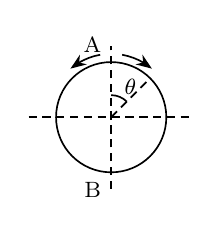
\begin{tikzpicture}[scale=0.7]
\draw (0,0) circle (1); \draw[densely dashed] (-1.5,0) -- (1.5,0) (0,-1.3) -- (0,1.3);
\node[lbl,above left] at (0,1) {A}; \node[lbl,below left] at (0,-1) {B};
\draw[densely dashed] (0,0) -- (45:1); \draw (0,0.4) arc (90:45:0.4); \node[lbl] at (0.35,0.55) {$\theta$};
\draw[->] (100:1.15) arc (100:130:1.15); \draw[->] (80:1.15) arc (80:50:1.15);
\end{tikzpicture}}\ntag{A}{53}{keph104}{5}{}{Class XI Part 1 \textperiodcentered{} Ch 4}}
{\optfig{\gaxes{$\theta$}{$P$}{\draw (0,1.2) -- (1.6,1.2); \node[font=\tiny,below] at (0,0) {$\frac\pi2$}; \node[font=\tiny,below] at (1.6,0) {$-\frac\pi2$};}}
{\gaxes{$\theta$}{$P$}{\draw (0,1.3) .. controls (0.2,0.4) and (0.6,0.05) .. (0.8,0) .. controls (1.0,0.05) and (1.4,0.4) .. (1.6,1.3); \node[font=\tiny,below] at (0,0) {$\frac\pi2$}; \node[font=\tiny,below] at (1.6,0) {$-\frac\pi2$};}}
{\gaxes{$\theta$}{$P$}{\draw (0,0) .. controls (0,0.9) and (0.35,1.3) .. (0.8,1.3) .. controls (1.25,1.3) and (1.6,0.9) .. (1.6,0); \node[font=\tiny,below] at (0,0) {$\frac\pi2$}; \node[font=\tiny,below] at (1.6,0) {$-\frac\pi2$};}}
{\gaxes{$\theta$}{$P$}{\draw (0,1.4) -- (1.6,0); \node[font=\tiny,below] at (0,0) {$\frac\pi2$}; \node[font=\tiny,below] at (1.6,0) {$-\frac\pi2$};}}}
\topichead{Impulse and momentum}{3}
\numoptstrue
\QQ{\qsrc{2025}{10}A ball of mass $0.5\unit{kg}$ is dropped from a height of $40\unit{m}$. The ball hits the ground and rises to a height of $10\unit{m}$. The impulse imparted to the ball during its collision with the ground is (Take $g = 9.8\unit{m/s^2}$)\ntag{A}{55}{keph104}{7}{}{Class XI Part 1 \textperiodcentered{} Ch 4}}
{\opt{21\,N\,s}{7\,N\,s}{0}{84\,N\,s}}
\numoptstrue
\QQ{\qsrc{2023}{13}A football player is moving southward and suddenly turns eastward with the same speed to avoid an opponent. The force that acts on the player while turning is:\ntag{A}{54}{keph104}{6}{}{Class XI Part 1 \textperiodcentered{} Ch 4}}
{\opt{along south-west}{along eastward}{along northward}{along north-east}}
\numoptstrue
\QQ{\qsrc{2021}{45}A ball of mass $0.15\unit{kg}$ is dropped from a height $10\unit{m}$, strikes the ground and rebounds to the same height. The magnitude of impulse imparted to the ball is ($g = 10\unit{m/s^2}$) nearly:\ntag{A}{55}{keph104}{7}{}{Class XI Part 1 \textperiodcentered{} Ch 4}}
{\opt{0\,kg\,m/s}{4.2\,kg\,m/s}{2.1\,kg\,m/s}{1.4\,kg\,m/s}}
\topichead{Laws of motion (lift, apparent weight)}{3}
\numoptstrue
\QQ{\qsrc{2024}{31}A horizontal force $10\unit{N}$ is applied to a block A as shown in figure. The mass of blocks A and B are $2\unit{kg}$ and $3\unit{kg}$, respectively. The blocks slide over a frictionless surface. The force exerted by block A on block B is:
\fig{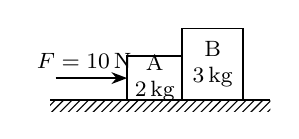
\begin{tikzpicture}[scale=0.7]
\fill[pattern=north east lines] (-0.4,-0.2) rectangle (3.6,0); \draw (-0.4,0) -- (3.6,0);
\draw (1,0) rectangle (2,0.8) node[midway,lbl,align=center]{A\\2\,kg}; \draw (2,0) rectangle (3.1,1.3) node[midway,lbl,align=center]{B\\3\,kg};
\draw[->] (-0.3,0.4) -- (1,0.4) node[pos=0.4,above,lbl]{$F = 10\unit{N}$};
\end{tikzpicture}}\ntag{A}{54}{keph104}{6}{}{Class XI Part 1 \textperiodcentered{} Ch 4}}
{\opt{10\,N}{zero}{4\,N}{6\,N}}
\numoptstrue
\QQ{\qsrc{2020}{160}Two bodies of mass $4\unit{kg}$ and $6\unit{kg}$ are tied to the ends of a massless string. The string passes over a pulley which is frictionless (see figure). The acceleration of the system in terms of acceleration due to gravity ($g$) is:
\fig{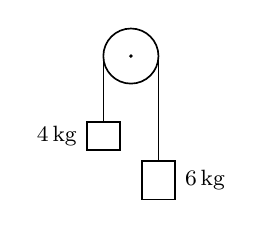
\begin{tikzpicture}[scale=0.7]
\draw (0,0) circle (0.5); \fill (0,0) circle (1pt); \draw (-0.5,0) -- (-0.5,-1.2); \draw (0.5,0) -- (0.5,-1.9);
\draw (-0.8,-1.2) rectangle (-0.2,-1.7); \node[lbl,left] at (-0.8,-1.45) {4\,kg};
\draw (0.2,-1.9) rectangle (0.8,-2.6); \node[lbl,right] at (0.8,-2.25) {6\,kg};
\end{tikzpicture}}\ntag{D}{70}{keph104}{22}{ \textperiodcentered{} Exercise 4.16}{Class XI Part 1 \textperiodcentered{} Ch 4}}
{\opt{$g$}{$g/2$}{$g/5$}{$g/10$}}
\numoptstrue
\QQ{\qsrc{2018}{35}A block of mass $m$ is placed on a smooth inclined wedge ABC of inclination $\theta$ as shown in the figure. The wedge is given an acceleration `$a$' towards the right. The relation between $a$ and $\theta$ for the block to remain stationary on the wedge is
\fig{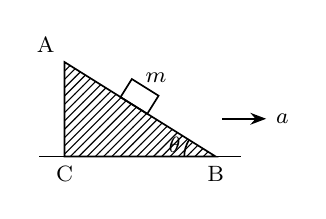
\begin{tikzpicture}[scale=0.8]
\fill[pattern=north east lines] (0,0) -- (0,1.5) -- (2.4,0) -- cycle; \draw (0,0) -- (0,1.5) -- (2.4,0) -- cycle; \draw (-0.4,0) -- (2.8,0);
\node[lbl,above left] at (0,1.5) {A}; \node[lbl,below] at (0,0) {C}; \node[lbl,below] at (2.4,0) {B};
\draw[rotate around={-32:(1.1,0.81)}] (0.85,0.81) rectangle (1.35,1.15); \node[lbl] at (1.45,1.25) {$m$};
\draw (1.9,0) arc (180:148:0.5); \node[lbl] at (1.75,0.18) {$\theta$}; \draw[->] (2.5,0.6) -- (3.2,0.6) node[right,lbl]{$a$};
\end{tikzpicture}}\ntag{A}{65}{keph104}{17}{}{Class XI Part 1 \textperiodcentered{} Ch 4}}
{\opt{$a = g\cos\theta$}{$a = \dfrac g{\sin\theta}$}{$a = \dfrac g{\operatorname{cosec}\theta}$}{$a = g\tan\theta$}}
\topichead{Collisions and momentum conservation}{1}
\numoptstrue
\QQ{\qsrc{2022}{20}A shell of mass $m$ is at rest initially. It explodes into three fragments having mass in the ratio $2:2:1$. If the fragments having equal mass fly off along mutually perpendicular directions with speed $v$, the speed of the third (lighter) fragment is:\ntag{A}{57}{keph104}{9}{}{Class XI Part 1 \textperiodcentered{} Ch 4}}
{\opt{$3\sqrt2\,v$}{$v$}{$\sqrt2\,v$}{$2\sqrt2\,v$}}
\topichead{Equilibrium of forces and tension}{2}
\numoptstrue
\QQ{\qsrc{2019}{33}A particle moving with velocity $\vec V$ is acted by three forces shown by the vector triangle PQR. The velocity of the particle will:
\fig{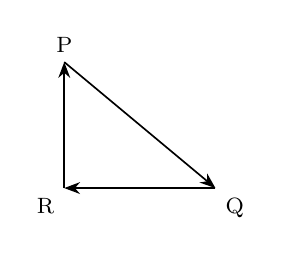
\begin{tikzpicture}[scale=0.8]
\coordinate (P) at (0,2); \coordinate (Q) at (2.4,0); \coordinate (R) at (0,0);
\draw[->] (P) -- (Q); \draw[->] (Q) -- (R); \draw[->] (R) -- (P);
\node[lbl,above] at (P) {P}; \node[lbl,below right] at (Q) {Q}; \node[lbl,below left] at (R) {R};
\end{tikzpicture}}\ntag{D}{58}{keph104}{10}{ \textperiodcentered{} forces forming a closed triangle}{Class XI Part 1 \textperiodcentered{} Ch 4}}
{\opt{increase}{decrease}{remain constant}{change according to the smallest force $\overrightarrow{QR}$}}
\numoptstrue
\QQ{\qsrc{2017}{167}Two blocks A and B of masses $3m$ and $m$ respectively are connected by a massless and inextensible string. The whole system is suspended by a massless spring as shown in figure. The magnitudes of acceleration of A and B immediately after the string is cut, are respectively:
\fig{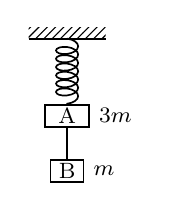
\begin{tikzpicture}[scale=0.7]
\fill[pattern=north east lines] (-0.7,2.6) rectangle (0.7,2.8); \draw (-0.7,2.6) -- (0.7,2.6);
\draw[decorate,decoration={coil,aspect=0.5,segment length=3pt,amplitude=4pt}] (0,2.6) -- (0,1.4);
\draw (-0.4,1.0) rectangle (0.4,1.4) node[midway,lbl]{A}; \node[lbl,right] at (0.4,1.2) {$3m$}; \draw (0,1.0) -- (0,0.4);
\draw (-0.3,0) rectangle (0.3,0.4) node[midway,lbl]{B}; \node[lbl,right] at (0.3,0.2) {$m$};
\end{tikzpicture}}\ntag{A}{59}{keph104}{11}{ \textperiodcentered{} spring force}{Class XI Part 1 \textperiodcentered{} Ch 4}}
{\opt{$\dfrac g3$, $g$}{$g$, $g$}{$\dfrac g3$, $\dfrac g3$}{$g$, $\dfrac g3$}}
\topichead{Friction}{4}
\numoptstrue
\QQ{\qsrc{2025}{4}There are two inclined surfaces of equal length ($L$) and same angle of inclination $45^\circ$ with the horizontal. One of them is rough and the other is perfectly smooth. A given body takes 2 times as much time to slide down on rough surface than on the smooth surface. The coefficient of kinetic friction ($\mu_k$) between the object and the rough surface is close to\ntag{A}{61}{keph104}{13}{}{Class XI Part 1 \textperiodcentered{} Ch 4}}
{\opt{0.25}{0.40}{0.5}{0.75}}
\numoptstrue
\QQ{\qsrc{2023}{41}Calculate the maximum acceleration of a moving car so that a body lying on the floor of the car remains stationary. The coefficient of static friction between the body and the floor is 0.15 ($g = 10\unit{m\,s^{-2}}$).\ntag{D}{61}{keph104}{13}{ \textperiodcentered{} Example 4.7}{Class XI Part 1 \textperiodcentered{} Ch 4}}
{\opt{$50\unit{m\,s^{-2}}$}{$1.2\unit{m\,s^{-2}}$}{$150\unit{m\,s^{-2}}$}{$1.5\unit{m\,s^{-2}}$}}
\numoptstrue
\QQ{\qsrc{2019}{35}A block of mass $10\unit{kg}$ is in contact against the inner wall of a hollow cylindrical drum of radius $1\unit{m}$. The coefficient of friction between the block and the inner wall of the cylinder is 0.1. The minimum angular velocity needed for the cylinder to keep the block stationary when the cylinder is vertical and rotating about its axis, will be: ($g = 10\unit{m/s^2}$)\ntag{A}{63}{keph104}{15}{}{Class XI Part 1 \textperiodcentered{} Ch 4}}
{\opt{$\sqrt{10}$\,rad/s}{$\dfrac{10}{2\pi}$\,rad/s}{10\,rad/s}{$10\pi$\,rad/s}}
\numoptstrue
\QQ{\qsrc{2018}{33}Which one of the following statements is \textit{incorrect}?\ntag{D}{60}{keph104}{12}{ \textperiodcentered{} mu is dimensionless}{Class XI Part 1 \textperiodcentered{} Ch 4}}
{\opt{Frictional force opposes the relative motion.}{Limiting value of static friction is directly proportional to normal reaction.}{Rolling friction is smaller than sliding friction.}{Coefficient of sliding friction has dimensions of length.}}
\topichead{Circular motion}{4}
\numoptstrue
\QQ{\qsrc{2026}{41}A car travels on a circular racetrack of radius $50\unit{m}$, which is banked at an angle $\theta$. If the car travels at a speed $10\unit{m\,s^{-1}}$, then the wear and tear on its tyres is minimum. Taking the acceleration due to gravity to be $10\unit{m\,s^{-2}}$, the value of $\theta$ is:\ntag{D}{64}{keph104}{16}{ \textperiodcentered{} v0=sqrt(Rg tan theta)}{Class XI Part 1 \textperiodcentered{} Ch 4}}
{\opt{$\tan^{-1}\!\left(\dfrac15\right)$}{$\tan^{-1}\!\left(\dfrac25\right)$}{$\tan^{-1}(\sqrt3/2)$}{$\tan^{-1}(2\sqrt3)$}}
\numoptstrue
\QQ{\qsrc{2024}{25}A bob is whirled in a horizontal plane by means of a string with an initial speed of $\omega$ rpm. The tension in the string is $T$. If speed becomes $2\omega$ while keeping the same radius, the tension in the string becomes:\ntag{A}{63}{keph104}{15}{}{Class XI Part 1 \textperiodcentered{} Ch 4}}
{\opt{$\sqrt2T$}{$T$}{$4T$}{$\dfrac T4$}}
\numoptstrue
\QQ{\qsrc{2017}{156}One end of string of length $l$ is connected to a particle of mass `$m$' and the other end is connected to a small peg on a smooth horizontal table. If the particle moves in circle with speed `$v$', the net force on the particle (directed towards center) will be ($T$ represents the tension in the string):\ntag{D}{69}{keph104}{21}{ \textperiodcentered{} Exercise 4.4}{Class XI Part 1 \textperiodcentered{} Ch 4}}
{\opt{$T+\dfrac{mv^2}l$}{$T-\dfrac{mv^2}l$}{Zero}{$T$}}
\numoptstrue
\QQ{\qsrc{2016}{45}A car is negotiating a curved road of radius $R$. The road is banked at an angle $\theta$. The coefficient of friction between the tyres of the car and the road is $\mu_s$. The maximum safe velocity on this road is:\ntag{D}{64}{keph104}{16}{ \textperiodcentered{} banked road}{Class XI Part 1 \textperiodcentered{} Ch 4}}
{\opt{$\sqrt{gR^2\dfrac{\mu_s+\tan\theta}{1-\mu_s\tan\theta}}$}{$\sqrt{gR\dfrac{\mu_s+\tan\theta}{1-\mu_s\tan\theta}}$}{$\sqrt{\dfrac gR\dfrac{\mu_s+\tan\theta}{1-\mu_s\tan\theta}}$}{$\sqrt{\dfrac g{R^2}\dfrac{\mu_s+\tan\theta}{1-\mu_s\tan\theta}}$}}
\end{multicols}
\par\needspace{12\baselineskip}\vspace{12pt}
\begin{center}{\pgfornament[width=3.2cm,color=gilt]{87}}\par
{\large\color{navy}\scshape Laws of Motion \textperiodcentered{} Answer Key}\end{center}
{\small\setlength{\tabcolsep}{1pt}\renewcommand{\arraystretch}{1.5}
\begin{tabularx}{\linewidth}{@{}*{8}{>{\centering\arraybackslash}X}@{}}\toprule
\textbf{1}\,(3) & \textbf{2}\,(1) & \textbf{3}\,(4) & \textbf{4}\,(2) & \textbf{5}\,(4) & \textbf{6}\,(3) & \textbf{7}\,(4) & \textbf{8}\,(4)\\
\textbf{9}\,(3) & \textbf{10}\,(1) & \textbf{11}\,(4) & \textbf{12}\,(4) & \textbf{13}\,(3) & \textbf{14}\,(4) & \textbf{15}\,(1) & \textbf{16}\,(3)\\
\textbf{17}\,(4) & \textbf{18}\,(2) &  &  &  &  &  & \\\bottomrule\end{tabularx}}\par\smallskip
{\footnotesize Answers of 2021, 2022, 2023, 2025 and 2026 are from the official NTA final keys (checked by the editor); answers of 2016--2020 and 2024 were solved by the editor.
}\par
\par\needspace{18\baselineskip}\vspace{14pt}
\begin{center}{\pgfornament[width=3.2cm,color=gilt]{87}}\par
{\large\color{navy}\scshape Chapter Summary \textperiodcentered{} Laws of Motion}\end{center}
{\small\setlength{\tabcolsep}{3.5pt}
\begin{tabular*}{\linewidth}{@{\extracolsep{\fill}}l*{11}{c}c@{}}\toprule
Year & 2016 & 2017 & 2018 & 2019 & 2020 & 2021 & 2022 & 2023 & 2024 & 2025 & 2026 & Total\\\midrule
Questions & 1 & 2 & 2 & 2 & 1 & 1 & 1 & 2 & 2 & 2 & 2 & \textbf{18}\\\bottomrule\end{tabular*}}\par\medskip
{\small\textbf{\color{crimson}Topic-wise} (in textbook order)\par\smallskip
\begin{tabularx}{\linewidth}{@{}>{\raggedright\arraybackslash}Xrrrl@{}}\toprule
Topic & Qs & Direct & Years & 2016 $\rightarrow$ 2026\\\midrule
Kinetic energy and momentum & \textbf{1} & 0 & 1 & {\scriptsize {\color{gray!45}16} {\color{gray!45}17} {\color{gray!45}18} {\color{gray!45}19} {\color{gray!45}20} {\color{gray!45}21} {\color{gray!45}22} {\color{gray!45}23} {\color{gray!45}24} {\color{gray!45}25} \textbf{26}}\\
Impulse and momentum & \textbf{3} & 0 & 3 & {\scriptsize {\color{gray!45}16} {\color{gray!45}17} {\color{gray!45}18} {\color{gray!45}19} {\color{gray!45}20} \textbf{21} {\color{gray!45}22} \textbf{23} {\color{gray!45}24} \textbf{25} {\color{gray!45}26}}\\
Laws of motion (lift, apparent weight) & \textbf{3} & 1 & 3 & {\scriptsize {\color{gray!45}16} {\color{gray!45}17} \textbf{18} {\color{gray!45}19} \textbf{20} {\color{gray!45}21} {\color{gray!45}22} {\color{gray!45}23} \textbf{24} {\color{gray!45}25} {\color{gray!45}26}}\\
Collisions and momentum conservation & \textbf{1} & 0 & 1 & {\scriptsize {\color{gray!45}16} {\color{gray!45}17} {\color{gray!45}18} {\color{gray!45}19} {\color{gray!45}20} {\color{gray!45}21} \textbf{22} {\color{gray!45}23} {\color{gray!45}24} {\color{gray!45}25} {\color{gray!45}26}}\\
Equilibrium of forces and tension & \textbf{2} & 1 & 2 & {\scriptsize {\color{gray!45}16} \textbf{17} {\color{gray!45}18} \textbf{19} {\color{gray!45}20} {\color{gray!45}21} {\color{gray!45}22} {\color{gray!45}23} {\color{gray!45}24} {\color{gray!45}25} {\color{gray!45}26}}\\
Friction & \textbf{4} & 2 & 4 & {\scriptsize {\color{gray!45}16} {\color{gray!45}17} \textbf{18} \textbf{19} {\color{gray!45}20} {\color{gray!45}21} {\color{gray!45}22} \textbf{23} {\color{gray!45}24} \textbf{25} {\color{gray!45}26}}\\
Circular motion & \textbf{4} & 3 & 4 & {\scriptsize \textbf{16} \textbf{17} {\color{gray!45}18} {\color{gray!45}19} {\color{gray!45}20} {\color{gray!45}21} {\color{gray!45}22} {\color{gray!45}23} \textbf{24} {\color{gray!45}25} \textbf{26}}\\
\bottomrule\end{tabularx}}\par\medskip
\begin{minipage}[t]{0.34\linewidth}{\small\textbf{\color{crimson}Direct vs Applied}\par\smallskip
\begin{tabular}{@{}lrr@{}}\toprule
Direct from NCERT & \textbf{7} & 39\%\\
\quad text, table, figure & 4 &\\
\quad solved Example & 1 &\\
\quad Exercise & 2 &\\
Applied & \textbf{11} & 61\%\\\midrule
Easy / Mod. / Hard & \multicolumn{2}{r}{11 / 7 / 0}\\\bottomrule
\end{tabular}}\end{minipage}\hfill
\begin{minipage}[t]{0.63\linewidth}{\small\textbf{\color{crimson}What to focus on}\par\smallskip
\begin{itemize}[leftmargin=1.1em,itemsep=1pt,topsep=0pt]
\item 18 questions in 11 papers, about 1.6 per paper; rank 9 of 28 chapters by number of questions.
\item Most asked topic: \textbf{Friction} (4 questions, in 4 of the 11 years).
\item 3 questions are NCERT solved Examples or Exercises: Example 4.7 (Q 12), Exercise 4.16 (Q 6), Exercise 4.4 (Q 17). Work these by hand.
\item Difficulty: 11 easy, 7 moderate, 0 hard.
\item 11 applied questions: practise these after the NCERT Examples and Exercises of the chapter.
\end{itemize}}\end{minipage}\par
\chapterpaper{Class XI \textperiodcentered{} Chapter 5}{Work, Energy and Power}{18 questions \textperiodcentered{} 3 topics \textperiodcentered{} NEET 2016--2026}{ckeph105}{XI.5 Work, Energy and Power}
\begin{multicols}{2}
\topichead{Work-energy theorem and power}{11}
\numoptstrue
\QQ{\qsrc{2026}{1}A particle of mass $M$ moves along a horizontal $x$ axis from $x = 0$ to $x = L$. The coefficient of kinetic friction varies as a function of $x$ as $\mu_k(x) = \mu_0 - \alpha x$, where $\mu_0$, $\alpha$ are constants of appropriate dimensions, so that $\mu_k(L) = 0$. The total work done by the frictional force during the motion is $n\mu_0MgL$, where $g$ is the acceleration due to gravity. The value of $n$ is:\ntag{A}{75}{keph105}{5}{ \textperiodcentered{} work by variable force (area under F-x)}{Class XI Part 1 \textperiodcentered{} Ch 5}}
{\opt{3}{1}{$\dfrac13$}{$\dfrac12$}}
\numoptstrue
\QQ{\qsrc{2025}{5}The kinetic energies of two similar cars A and B are $100\unit{J}$ and $225\unit{J}$ respectively. On applying brakes, car A stops after $1000\unit{m}$ and car B stops after $1500\unit{m}$. If $F_A$ and $F_B$ are the forces applied by the brakes on cars A and B, respectively, then the ratio $F_A/F_B$ is\ntag{A}{73}{keph105}{3}{}{Class XI Part 1 \textperiodcentered{} Ch 5}}
{\opt{$\dfrac32$}{$\dfrac23$}{$\dfrac13$}{$\dfrac12$}}
\numoptstrue
\QQ{\qsrc{2024}{13}At any instant of time $t$, the displacement of any particle is given by $2t-1$ (SI unit) under the influence of force of $5\unit{N}$. The value of instantaneous power is (in SI unit):\ntag{D}{83}{keph105}{13}{ \textperiodcentered{} P=F.v}{Class XI Part 1 \textperiodcentered{} Ch 5}}
{\opt{6}{10}{5}{7}}
\numoptstrue
\QQ{\qsrc{2023}{29}The potential energy of a long spring when stretched by $2\unit{cm}$ is U. If the spring is stretched by $8\unit{cm}$, potential energy stored in it will be:\ntag{D}{81}{keph105}{11}{ \textperiodcentered{} U=kx\textasciicircum{}2/2}{Class XI Part 1 \textperiodcentered{} Ch 5}}
{\opt{16U}{2U}{4U}{8U}}
\numoptstrue
\QQ{\qsrc{2022}{15}The energy that will be ideally radiated by a $100\unit{kW}$ transmitter in 1 hour is:\ntag{D}{83}{keph105}{13}{ \textperiodcentered{} energy = power x time}{Class XI Part 1 \textperiodcentered{} Ch 5}}
{\opt{$1\times10^5\unit{J}$}{$36\times10^7\unit{J}$}{$36\times10^4\unit{J}$}{$36\times10^5\unit{J}$}}
\numoptstrue
\QQ{\qsrc{2022}{16}An electric lift with a maximum load of $2000\unit{kg}$ (lift + passengers) is moving up with a constant speed of $1.5\unit{m\,s^{-1}}$. The frictional force opposing the motion is $3000\unit{N}$. The minimum power delivered by the motor to the lift in watts is: ($g = 10\unit{m\,s^{-2}}$)\ntag{D}{83}{keph105}{13}{ \textperiodcentered{} Example 5.10}{Class XI Part 1 \textperiodcentered{} Ch 5}}
{\opt{23500}{23000}{20000}{34500}}
\numoptstrue
\QQ{\qsrc{2021}{11}A particle is released from height $S$ from the surface of the Earth. At a certain height its kinetic energy is three times its potential energy. The height from the surface of earth and the speed of the particle at that instant are respectively:\ntag{A}{78}{keph105}{8}{}{Class XI Part 1 \textperiodcentered{} Ch 5}}
{\opt{$\dfrac S4,\ \dfrac{3gS}2$}{$\dfrac S4,\ \dfrac{\sqrt{3gS}}2$}{$\dfrac S2,\ \dfrac{\sqrt{3gS}}2$}{$\dfrac S4,\ \sqrt{\dfrac{3gS}2}$}}
\numoptstrue
\QQ{\qsrc{2021}{23}Water falls from a height of $60\unit{m}$ at the rate of $15\unit{kg/s}$ to operate a turbine. The losses due to frictional force are 10\% of the input energy. How much power is generated by the turbine? ($g = 10\unit{m/s^2}$)\ntag{A}{83}{keph105}{13}{}{Class XI Part 1 \textperiodcentered{} Ch 5}}
{\opt{10.2\,kW}{8.1\,kW}{12.3\,kW}{7.0\,kW}}
\numoptstrue
\QQ{\qsrc{2019}{22}A force $F = 20+10y$ acts on a particle in $y$-direction where $F$ is in newton and $y$ in meter. Work done by this force to move the particle from $y = 0$ to $y = 1\unit{m}$ is:\ntag{D}{75}{keph105}{5}{ \textperiodcentered{} W = integral of F dx}{Class XI Part 1 \textperiodcentered{} Ch 5}}
{\opt{30\,J}{5\,J}{25\,J}{20\,J}}
\numoptstrue
\QQ{\qsrc{2017}{177}Consider a drop of rain water having mass 1\,g falling from a height of 1\,km. It hits the ground with a speed of $50\unit{m/s}$. Take `$g$' constant with a value $10\unit{m/s^2}$. The work done by the (i) gravitational force and the (ii) resistive force of air is:\ntag{D}{73}{keph105}{3}{ \textperiodcentered{} Example 5.2}{Class XI Part 1 \textperiodcentered{} Ch 5}}
{\opt{(i) 1.25\,J (ii) $-8.25$\,J}{(i) 100\,J (ii) 8.75\,J}{(i) 10\,J (ii) $-8.75$\,J}{(i) $-10$\,J (ii) $-8.25$\,J}}
\numoptstrue
\QQ{\qsrc{2016}{39}A body of mass 1\,kg begins to move under the action of a time dependent force $\vec F = (2t\hat i+3t^2\hat j)\unit{N}$, where $\hat i$ and $\hat j$ are unit vectors along $x$ and $y$ axis. What power will be developed by the force at the time $t$?\ntag{A}{83}{keph105}{13}{ \textperiodcentered{} P=F.v}{Class XI Part 1 \textperiodcentered{} Ch 5}}
{\opt{$(2t^2+3t^3)$\,W}{$(2t^2+4t^4)$\,W}{$(2t^3+3t^4)$\,W}{$(2t^3+3t^5)$\,W}}
\topichead{Circular motion}{4}
\numoptstrue
\QQ{\qsrc{2025}{7}A bob of heavy mass $m$ is suspended by a light string of length $l$. The bob is given a horizontal velocity $v_0$ as shown in figure. If the string gets slack at some point P making an angle $\theta$ from the horizontal, the ratio of the speed $v$ of the bob at point P to its initial speed $v_0$ is:
\fig{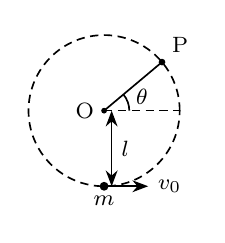
\begin{tikzpicture}[scale=0.8]
\draw[densely dashed] (0,0) circle (1.2); \fill (0,0) circle (1.3pt) node[left,lbl]{O};
\draw[<->] (0.12,0) -- (0.12,-1.2) node[midway,right,lbl]{$l$};
\fill (0,-1.2) circle (2pt) node[below,lbl]{$m$}; \draw[->] (0,-1.2) -- (0.7,-1.2) node[right,lbl]{$v_0$};
\draw (0,0) -- (40:1.2); \fill (40:1.2) circle (1.5pt) node[above right,lbl]{P};
\draw[densely dashed] (0,0) -- (1.2,0); \draw (0.4,0) arc (0:40:0.4); \node[lbl] at (0.6,0.22) {$\theta$};
\end{tikzpicture}}\ntag{A}{79}{keph105}{9}{ \textperiodcentered{} Example 5.7 setting}{Class XI Part 1 \textperiodcentered{} Ch 5}}
{\opt{$(\sin\theta)^{1/2}$}{$\left(\dfrac1{2+3\sin\theta}\right)^{1/2}$}{$\left(\dfrac{\cos\theta}{2+3\sin\theta}\right)^{1/2}$}{$\left(\dfrac{\sin\theta}{2+3\sin\theta}\right)^{1/2}$}}
\numoptstrue
\QQ{\qsrc{2019}{2}A mass $m$ is attached to a thin wire and whirled in a vertical circle. The wire is most likely to break when:\ntag{A}{79}{keph105}{9}{ \textperiodcentered{} vertical circle (Example 5.7)}{Class XI Part 1 \textperiodcentered{} Ch 5}}
{\opt{the mass is at the highest point}{the wire is horizontal}{the mass is at the lowest point}{inclined at an angle of $60^\circ$ from vertical}}
\numoptstrue
\QQ{\qsrc{2018}{30}A body initially at rest and sliding along a frictionless track from a height $h$ (as shown in the figure) just completes a vertical circle of diameter $AB = D$. The height $h$ is equal to
\fig{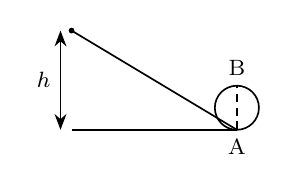
\begin{tikzpicture}[scale=0.7]
\draw (0,0) -- (3,0); \draw (0,1.8) -- (3,0); \fill (0,1.8) circle (1.5pt); \draw[<->] (-0.2,0) -- (-0.2,1.8) node[midway,left,lbl]{$h$};
\draw (3,0.4) circle (0.4); \node[lbl,below] at (3,0) {A}; \node[lbl,above] at (3,0.8) {B}; \draw[densely dashed] (3,0) -- (3,0.8);
\end{tikzpicture}}\ntag{A}{79}{keph105}{9}{ \textperiodcentered{} Example 5.7 setting}{Class XI Part 1 \textperiodcentered{} Ch 5}}
{\opt{$\dfrac75D$}{$D$}{$\dfrac32D$}{$\dfrac54D$}}
\numoptstrue
\QQ{\qsrc{2016}{28}What is the minimum velocity with which a body of mass $m$ must enter a vertical loop of radius $R$ so that it can complete the loop?\ntag{D}{79}{keph105}{9}{ \textperiodcentered{} Example 5.7}{Class XI Part 1 \textperiodcentered{} Ch 5}}
{\opt{$\sqrt{gR}$}{$\sqrt{2gR}$}{$\sqrt{3gR}$}{$\sqrt{5gR}$}}
\topichead{Collisions and momentum conservation}{3}
\numoptstrue
\QQ{\qsrc{2026}{44}Bob B of mass $m$ at rest is hanging vertically from the ceiling via a massless string of length $10\unit{m}$, as shown in the figure. Point mass A of mass $m$ travelling horizontally with speed $10\unit{m\,s^{-1}}$ hits bob B elastically. The bob B rises $h$ metre after the collision. Taking the acceleration due to gravity $g = 10\unit{m\,s^{-2}}$ and neglecting the size of the bob, the value of $h$ is:
\fig{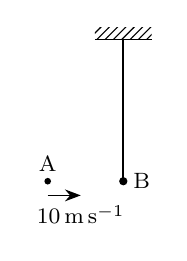
\begin{tikzpicture}[scale=0.6]
\fill[pattern=north east lines] (-0.6,3) rectangle (0.6,3.25); \draw (-0.6,3) -- (0.6,3);
\draw (0,3) -- (0,0); \fill (0,0) circle (2.5pt) node[right,lbl]{B};
\fill (-1.6,0) circle (2pt) node[above,lbl]{A}; \draw[->] (-1.6,-0.3) -- (-0.9,-0.3) node[below,lbl]{$10\unit{m\,s^{-1}}$};
\end{tikzpicture}}\ntag{A}{84}{keph105}{14}{}{Class XI Part 1 \textperiodcentered{} Ch 5}}
{\opt{8}{7}{5}{2.5}}
\numoptstrue
\QQ{\qsrc{2024}{29}Two bodies A and B of same mass undergo completely inelastic one dimensional collision. The body A moves with velocity $v_1$ while body B is at rest before collision. The velocity of the system after collision is $v_2$. The ratio $v_1:v_2$ is:\ntag{D}{84}{keph105}{14}{ \textperiodcentered{} completely inelastic collision}{Class XI Part 1 \textperiodcentered{} Ch 5}}
{\opt{1:4}{1:2}{2:1}{4:1}}
\numoptstrue
\QQ{\qsrc{2019}{4}Body A of mass $4m$ moving with speed $u$ collides with another body B of mass $2m$, at rest. The collision is head on and elastic in nature. After the collision the fraction of energy lost by the colliding body A is:\ntag{A}{84}{keph105}{14}{}{Class XI Part 1 \textperiodcentered{} Ch 5}}
{\opt{$\dfrac19$}{$\dfrac89$}{$\dfrac49$}{$\dfrac59$}}
\end{multicols}
\par\needspace{12\baselineskip}\vspace{12pt}
\begin{center}{\pgfornament[width=3.2cm,color=gilt]{87}}\par
{\large\color{navy}\scshape Work, Energy and Power \textperiodcentered{} Answer Key}\end{center}
{\small\setlength{\tabcolsep}{1pt}\renewcommand{\arraystretch}{1.5}
\begin{tabularx}{\linewidth}{@{}*{8}{>{\centering\arraybackslash}X}@{}}\toprule
\textbf{1}\,(4) & \textbf{2}\,(2) & \textbf{3}\,(2) & \textbf{4}\,(1) & \textbf{5}\,(2) & \textbf{6}\,(4) & \textbf{7}\,(4) & \textbf{8}\,(2)\\
\textbf{9}\,(3) & \textbf{10}\,(3) & \textbf{11}\,(4) & \textbf{12}\,(4) & \textbf{13}\,(3) & \textbf{14}\,(4) & \textbf{15}\,(4) & \textbf{16}\,(3)\\
\textbf{17}\,(3) & \textbf{18}\,(2) &  &  &  &  &  & \\\bottomrule\end{tabularx}}\par\smallskip
{\footnotesize Answers of 2021, 2022, 2023, 2025 and 2026 are from the official NTA final keys (checked by the editor); answers of 2016--2020 and 2024 were solved by the editor.
}\par
\par\needspace{18\baselineskip}\vspace{14pt}
\begin{center}{\pgfornament[width=3.2cm,color=gilt]{87}}\par
{\large\color{navy}\scshape Chapter Summary \textperiodcentered{} Work, Energy and Power}\end{center}
{\small\setlength{\tabcolsep}{3.5pt}
\begin{tabular*}{\linewidth}{@{\extracolsep{\fill}}l*{11}{c}c@{}}\toprule
Year & 2016 & 2017 & 2018 & 2019 & 2020 & 2021 & 2022 & 2023 & 2024 & 2025 & 2026 & Total\\\midrule
Questions & 2 & 1 & 1 & 3 & 0 & 2 & 2 & 1 & 2 & 2 & 2 & \textbf{18}\\\bottomrule\end{tabular*}}\par\medskip
{\small\textbf{\color{crimson}Topic-wise} (in textbook order)\par\smallskip
\begin{tabularx}{\linewidth}{@{}>{\raggedright\arraybackslash}Xrrrl@{}}\toprule
Topic & Qs & Direct & Years & 2016 $\rightarrow$ 2026\\\midrule
Work-energy theorem and power & \textbf{11} & 6 & 9 & {\scriptsize \textbf{16} \textbf{17} {\color{gray!45}18} \textbf{19} {\color{gray!45}20} \textbf{21} \textbf{22} \textbf{23} \textbf{24} \textbf{25} \textbf{26}}\\
Circular motion & \textbf{4} & 1 & 4 & {\scriptsize \textbf{16} {\color{gray!45}17} \textbf{18} \textbf{19} {\color{gray!45}20} {\color{gray!45}21} {\color{gray!45}22} {\color{gray!45}23} {\color{gray!45}24} \textbf{25} {\color{gray!45}26}}\\
Collisions and momentum conservation & \textbf{3} & 1 & 3 & {\scriptsize {\color{gray!45}16} {\color{gray!45}17} {\color{gray!45}18} \textbf{19} {\color{gray!45}20} {\color{gray!45}21} {\color{gray!45}22} {\color{gray!45}23} \textbf{24} {\color{gray!45}25} \textbf{26}}\\
\bottomrule\end{tabularx}}\par\medskip
\begin{minipage}[t]{0.34\linewidth}{\small\textbf{\color{crimson}Direct vs Applied}\par\smallskip
\begin{tabular}{@{}lrr@{}}\toprule
Direct from NCERT & \textbf{8} & 44\%\\
\quad text, table, figure & 5 &\\
\quad solved Example & 3 &\\
\quad Exercise & 0 &\\
Applied & \textbf{10} & 56\%\\\midrule
Easy / Mod. / Hard & \multicolumn{2}{r}{9 / 8 / 1}\\\bottomrule
\end{tabular}}\end{minipage}\hfill
\begin{minipage}[t]{0.63\linewidth}{\small\textbf{\color{crimson}What to focus on}\par\smallskip
\begin{itemize}[leftmargin=1.1em,itemsep=1pt,topsep=0pt]
\item 18 questions in 11 papers, about 1.6 per paper; rank 10 of 28 chapters by number of questions.
\item Most asked topic: \textbf{Work-energy theorem and power} (11 questions, in 9 of the 11 years).
\item Asked in 8 or more of the 11 years: Work-energy theorem and power.
\item 3 questions are NCERT solved Examples or Exercises: Example 5.10 (Q 6), Example 5.2 (Q 10), Example 5.7 (Q 15). Work these by hand.
\item NCERT pages that gave three or more questions: page 83 (5 questions), page 79 (4 questions), page 84 (3 questions). Read these pages line by line.
\item Difficulty: 9 easy, 8 moderate, 1 hard (hard: Q 12).
\item 10 applied questions: practise these after the NCERT Examples and Exercises of the chapter.
\end{itemize}}\end{minipage}\par
\chapterpaper{Class XI \textperiodcentered{} Chapter 6}{System of Particles and Rotational Motion}{22 questions \textperiodcentered{} 3 topics \textperiodcentered{} NEET 2016--2026}{ckeph106}{XI.6 System of Particles and Rotational Motion}
\begin{multicols}{2}
\topichead{Rotational dynamics (torque, moment of inertia)}{15}
\numoptstrue
\QQ{\qsrc{2025}{22}A uniform rod of mass $20\unit{kg}$ and length $5\unit{m}$ leans against a smooth vertical wall making an angle of $60^\circ$ with it. The other end rests on a rough horizontal floor. The friction force that the floor exerts on the rod is (take $g = 10\unit{m/s^2}$)\ntag{A}{113}{keph106}{22}{}{Class XI Part 1 \textperiodcentered{} Ch 6}}
{\opt{100\,N}{$100\sqrt3$\,N}{200\,N}{$200\sqrt3$\,N}}
\numoptstrue
\QQ{\qsrc{2024}{10}The moment of inertia of a thin rod about an axis passing through its mid point and perpendicular to the rod is $2400\unit{g\,cm^2}$. The length of the 400\,g rod is nearly:\ntag{D}{116}{keph106}{25}{ \textperiodcentered{} Table 6.1}{Class XI Part 1 \textperiodcentered{} Ch 6}}
{\opt{72.0\,cm}{8.5\,cm}{17.5\,cm}{20.7\,cm}}
\numoptstrue
\QQ{\qsrc{2024}{32}A wheel of a bullock cart is rolling on a level road as shown in the figure below. If its linear speed is $v$ in the direction shown, which one of the following options is correct (P and Q are any highest and lowest points on the wheel, respectively)?
\fig{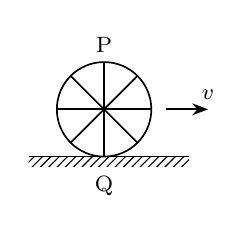
\begin{tikzpicture}[scale=0.6]
\fill[pattern=north east lines] (-1.6,-1.2) rectangle (1.8,-1.0); \draw (-1.6,-1) -- (1.8,-1);
\draw (0,0) circle (1); \foreach \a in {0,45,...,315} \draw (0,0) -- (\a:1);
\node[lbl,above] at (0,1) {P}; \node[lbl,below] at (0,-1.2) {Q}; \draw[->] (1.3,0) -- (2.2,0) node[above,lbl]{$v$};
\end{tikzpicture}}\ntag{A}{94}{keph106}{3}{ \textperiodcentered{} rolling (qualitative)}{Class XI Part 1 \textperiodcentered{} Ch 6}}
{\opt{Point P has zero speed.}{Point P moves slower than point Q.}{Point P moves faster than point Q.}{Both the points P and Q move with equal speed.}}
\numoptstrue
\QQ{\qsrc{2023}{15}The angular acceleration of a body, moving along the circumference of a circle, is:\ntag{D}{105}{keph106}{14}{ \textperiodcentered{} alpha along the axis}{Class XI Part 1 \textperiodcentered{} Ch 6}}
{\opt{along the axis of rotation}{along the radius, away from centre}{along the radius towards the centre}{along the tangent to its position}}
\numoptstrue
\QQ{\qsrc{2023}{32}The ratio of radius of gyration of a solid sphere of mass $M$ and radius $R$ about its own axis to the radius of gyration of the thin hollow sphere of same mass and radius about its axis is:\ntag{A}{115}{keph106}{24}{}{Class XI Part 1 \textperiodcentered{} Ch 6}}
{\opt{5:2}{3:5}{5:3}{2:5}}
\numoptstrue
\QQ{\qsrc{2022}{7}The ratio of the radius of gyration of a thin uniform disc about an axis passing through its centre and normal to its plane to the radius of gyration of the disc about its diameter is:\ntag{D}{116}{keph106}{25}{ \textperiodcentered{} Table 6.1 (k=R/sqrt2, R/2)}{Class XI Part 1 \textperiodcentered{} Ch 6}}
{\opt{$1:\sqrt2$}{2:1}{$\sqrt2:1$}{4:1}}
\numoptstrue
\QQ{\qsrc{2022}{22}The angular speed of a fly wheel moving with uniform angular acceleration changes from 1200\,rpm to 3120\,rpm in 16 seconds. The angular acceleration in $\mathrm{rad/s^2}$ is:\ntag{D}{117}{keph106}{26}{ \textperiodcentered{} Example 6.11}{Class XI Part 1 \textperiodcentered{} Ch 6}}
{\opt{$104\pi$}{$2\pi$}{$4\pi$}{$12\pi$}}
\numoptstrue
\QQ{\qsrc{2021}{40}A uniform rod of length $200\unit{cm}$ and mass $500\unit{g}$ is balanced on a wedge placed at $40\unit{cm}$ mark. A mass of $2\unit{kg}$ is suspended from the rod at $20\unit{cm}$ and another unknown mass `$m$' is suspended from the rod at $160\unit{cm}$ mark as shown in the figure. Find the value of `$m$' such that the rod is in equilibrium. ($g = 10\unit{m/s^2}$)
\fig{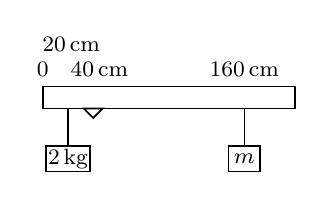
\begin{tikzpicture}[scale=0.8]
\draw (0,0) rectangle (4,0.35); \node[lbl,above] at (0,0.35) {0}; \node[lbl,above] at (0.45,0.75) {20\,cm}; \node[lbl,above] at (0.9,0.35) {40\,cm}; \node[lbl,above] at (3.2,0.35) {160\,cm};
\draw (0.8,-0.15) -- (0.95,0) -- (0.65,0) -- cycle; \draw (0.4,0) -- (0.4,-0.6); \draw (0.05,-0.6) rectangle (0.75,-1.0) node[midway,lbl]{2\,kg};
\draw (3.2,0) -- (3.2,-0.6); \draw (2.95,-0.6) rectangle (3.45,-1.0) node[midway,lbl]{$m$};
\end{tikzpicture}}\ntag{A}{111}{keph106}{20}{}{Class XI Part 1 \textperiodcentered{} Ch 6}}
{\opt{$\dfrac12$\,kg}{$\dfrac13$\,kg}{$\dfrac16$\,kg}{$\dfrac1{12}$\,kg}}
\numoptstrue
\QQ{\qsrc{2021}{50}From a circular ring of mass `$M$' and radius `$R$' an arc corresponding to a $90^\circ$ sector is removed. The moment of inertia of the remaining part of the ring about an axis passing through the centre of the ring and perpendicular to the plane of the ring is `$K$' times `$MR^2$'. Then the value of `$K$' is:\ntag{A}{115}{keph106}{24}{}{Class XI Part 1 \textperiodcentered{} Ch 6}}
{\opt{$\dfrac34$}{$\dfrac78$}{$\dfrac14$}{$\dfrac18$}}
\numoptstrue
\QQ{\qsrc{2020}{149}Find the torque about the origin when a force of $3\hat j\unit{N}$ acts on a particle whose position vector is $2\hat k\unit{m}$.\ntag{D}{103}{keph106}{12}{ \textperiodcentered{} vector product}{Class XI Part 1 \textperiodcentered{} Ch 6}}
{\opt{$6\hat i\unit{N\,m}$}{$6\hat j\unit{N\,m}$}{$-6\hat i\unit{N\,m}$}{$6\hat k\unit{N\,m}$}}
\numoptstrue
\QQ{\qsrc{2019}{21}A solid cylinder of mass $2\unit{kg}$ and radius $4\unit{cm}$ is rotating about its axis at the rate of 3\,rpm. The torque required to stop after $2\pi$ revolutions is:\ntag{A}{117}{keph106}{26}{}{Class XI Part 1 \textperiodcentered{} Ch 6}}
{\opt{$2\times10^{-6}\unit{N\,m}$}{$2\times10^{-3}\unit{N\,m}$}{$12\times10^{-4}\unit{N\,m}$}{$2\times10^6\unit{N\,m}$}}
\numoptstrue
\QQ{\qsrc{2018}{31}Three objects, A: (a solid sphere), B: (a thin circular disk) and C: (a circular ring), each have the same mass M and radius R. They all spin with the same angular speed $\omega$ about their own symmetry axes. The amounts of work ($W$) required to bring them to rest, would satisfy the relation\ntag{A}{116}{keph106}{25}{}{Class XI Part 1 \textperiodcentered{} Ch 6}}
{\opt{$W_B>W_A>W_C$}{$W_A>W_B>W_C$}{$W_C>W_B>W_A$}{$W_A>W_C>W_B$}}
\numoptstrue
\QQ{\qsrc{2018}{36}The moment of the force, $\vec F = 4\hat i+5\hat j-6\hat k$ at $(2,0,-3)$, about the point $(2,-2,-2)$, is given by\ntag{A}{106}{keph106}{15}{}{Class XI Part 1 \textperiodcentered{} Ch 6}}
{\opt{$-7\hat i-8\hat j-4\hat k$}{$-4\hat i-\hat j-8\hat k$}{$-8\hat i-4\hat j-7\hat k$}{$-7\hat i-4\hat j-8\hat k$}}
\numoptstrue
\QQ{\qsrc{2017}{161}A rope is wound around a hollow cylinder of mass $3\unit{kg}$ and radius $40\unit{cm}$. What is the angular acceleration of the cylinder if the rope is pulled with a force of $30\unit{N}$?\ntag{D}{126}{keph106}{35}{ \textperiodcentered{} Exercise 6.13}{Class XI Part 1 \textperiodcentered{} Ch 6}}
{\opt{$0.25\unit{rad/s^2}$}{$25\unit{rad/s^2}$}{$5\unit{m/s^2}$}{$25\unit{m/s^2}$}}
\numoptstrue
\QQ{\qsrc{2016}{19}A uniform circular disc of radius $50\unit{cm}$ at rest is free to turn about an axis which is perpendicular to its plane and passes through its centre. It is subjected to a torque which produces a constant angular acceleration of $2.0\unit{rad\,s^{-2}}$. Its net acceleration in $\mathrm{m\,s^{-2}}$ at the end of 2.0\,s is approximately:\ntag{A}{117}{keph106}{26}{ \textperiodcentered{} rotational kinematics, a\_t and a\_c}{Class XI Part 1 \textperiodcentered{} Ch 6}}
{\opt{8.0}{7.0}{6.0}{3.0}}
\topichead{Centre of mass}{3}
\numoptstrue
\QQ{\qsrc{2022}{14}Two objects of mass $10\unit{kg}$ and $20\unit{kg}$ respectively are connected to the two ends of a rigid rod of length $10\unit{m}$ with negligible mass. The distance of the center of mass of the system from the $10\unit{kg}$ mass is:\ntag{D}{96}{keph106}{5}{ \textperiodcentered{} two-particle CM}{Class XI Part 1 \textperiodcentered{} Ch 6}}
{\opt{5\,m}{$\dfrac{10}3$\,m}{$\dfrac{20}3$\,m}{10\,m}}
\numoptstrue
\QQ{\qsrc{2020}{148}Two particles of mass $5\unit{kg}$ and $10\unit{kg}$ respectively are attached to the two ends of a rigid rod of length $1\unit{m}$ with negligible mass. The centre of mass of the system from the $5\unit{kg}$ particle is nearly at a distance of:\ntag{D}{96}{keph106}{5}{ \textperiodcentered{} two-particle CM}{Class XI Part 1 \textperiodcentered{} Ch 6}}
{\opt{33\,cm}{50\,cm}{67\,cm}{80\,cm}}
\numoptstrue
\QQ{\qsrc{2017}{165}Which of the following statements are correct?
\begin{stmts}[(\alph*)]
\item Centre of mass of a body always coincides with the centre of gravity of the body.
\item Centre of mass of a body is the point at which the total gravitational torque on the body is zero.
\item A couple on a body produce both translational and rotational motion in a body.
\item Mechanical advantage greater than one means that small effort can be used to lift a large load.
\end{stmts}\ntag{D}{112}{keph106}{21}{ \textperiodcentered{} centre of gravity and mechanical advantage}{Class XI Part 1 \textperiodcentered{} Ch 6}}
{\opt{(a) and (b)}{(b) and (c)}{(c) and (d)}{(b) and (d)}}
\topichead{Angular momentum and its conservation}{4}
\numoptstrue
\QQ{\qsrc{2026}{31}A thin horizontal disc is rotating about a vertical axis passing through its fixed centre O. Its angular momentum is $L_A$ and $L_B$ computed about points A and B, respectively, with $OB = 2\times OA$. The value of $\dfrac{L_A}{L_B}$ is:
\fig{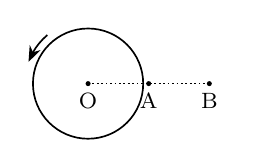
\begin{tikzpicture}[scale=0.7]
\draw (0,0) circle (1); \draw[->] (130:1.15) arc (130:160:1.15);
\fill (0,0) circle (1.3pt) node[below,lbl]{O}; \fill (1.1,0) circle (1.3pt) node[below,lbl]{A}; \fill (2.2,0) circle (1.3pt) node[below,lbl]{B};
\draw[densely dotted] (0,0) -- (2.2,0);
\end{tikzpicture}}\ntag{A}{108}{keph106}{17}{}{Class XI Part 1 \textperiodcentered{} Ch 6}}
{\opt{$\dfrac14$}{$\dfrac12$}{1}{2}}
\numoptstrue
\QQ{\qsrc{2025}{17}The Sun rotates around its centre once in 27 days. What will be the period of revolution if the Sun were to expand to twice its present radius without any external influence? Assume the Sun to be a sphere of uniform density.\ntag{A}{122}{keph106}{31}{}{Class XI Part 1 \textperiodcentered{} Ch 6}}
{\opt{100 days}{105 days}{115 days}{108 days}}
\numoptstrue
\QQ{\qsrc{2018}{38}A solid sphere is rotating freely about its symmetry axis in free space. The radius of the sphere is increased keeping its mass same. Which of the following physical quantities would remain constant for the sphere?\ntag{D}{108}{keph106}{17}{ \textperiodcentered{} L constant when torque is zero}{Class XI Part 1 \textperiodcentered{} Ch 6}}
{\opt{Rotational kinetic energy}{Moment of inertia}{Angular velocity}{Angular momentum}}
\numoptstrue
\QQ{\qsrc{2017}{162}Two discs of same moment of inertia rotating about their regular axis passing through centre and perpendicular to the plane of disc with angular velocities $\omega_1$ and $\omega_2$. They are brought into contact face to face coinciding the axis of rotation. The expression for loss of energy during this process is:\ntag{A}{122}{keph106}{31}{}{Class XI Part 1 \textperiodcentered{} Ch 6}}
{\opt{$\dfrac14I(\omega_1-\omega_2)^2$}{$I(\omega_1-\omega_2)^2$}{$\dfrac18(\omega_1-\omega_2)^2$}{$\dfrac12I(\omega_1+\omega_2)^2$}}
\end{multicols}
\par\needspace{12\baselineskip}\vspace{12pt}
\begin{center}{\pgfornament[width=3.2cm,color=gilt]{87}}\par
{\large\color{navy}\scshape System of Particles and Rotational Motion \textperiodcentered{} Answer Key}\end{center}
{\small\setlength{\tabcolsep}{1pt}\renewcommand{\arraystretch}{1.5}
\begin{tabularx}{\linewidth}{@{}*{8}{>{\centering\arraybackslash}X}@{}}\toprule
\textbf{1}\,(2) & \textbf{2}\,(2) & \textbf{3}\,(3) & \textbf{4}\,(1) & \textbf{5}\,(--)$^{*}$ & \textbf{6}\,(3) & \textbf{7}\,(3) & \textbf{8}\,(4)\\
\textbf{9}\,(1) & \textbf{10}\,(3) & \textbf{11}\,(1) & \textbf{12}\,(3) & \textbf{13}\,(4) & \textbf{14}\,(2) & \textbf{15}\,(1) & \textbf{16}\,(3)\\
\textbf{17}\,(3) & \textbf{18}\,(4) & \textbf{19}\,(3) & \textbf{20}\,(4) & \textbf{21}\,(4) & \textbf{22}\,(1) &  & \\\bottomrule\end{tabularx}}\par\smallskip
{\footnotesize Answers of 2021, 2022, 2023, 2025 and 2026 are from the official NTA final keys (checked by the editor); answers of 2016--2020 and 2024 were solved by the editor. --: question dropped by NTA. $^{*}$: see note.
\par\smallskip\textbf{5.} (NEET 2023 Q32) Dropped by NTA. The ratio is $\sqrt{2/5}:\sqrt{2/3}=\sqrt3:\sqrt5$, which is not among the options.
}\par
\par\needspace{18\baselineskip}\vspace{14pt}
\begin{center}{\pgfornament[width=3.2cm,color=gilt]{87}}\par
{\large\color{navy}\scshape Chapter Summary \textperiodcentered{} System of Particles and Rotational Motion}\end{center}
{\small\setlength{\tabcolsep}{3.5pt}
\begin{tabular*}{\linewidth}{@{\extracolsep{\fill}}l*{11}{c}c@{}}\toprule
Year & 2016 & 2017 & 2018 & 2019 & 2020 & 2021 & 2022 & 2023 & 2024 & 2025 & 2026 & Total\\\midrule
Questions & 1 & 3 & 3 & 1 & 2 & 2 & 3 & 2 & 2 & 2 & 1 & \textbf{22}\\\bottomrule\end{tabular*}}\par\medskip
{\small\textbf{\color{crimson}Topic-wise} (in textbook order)\par\smallskip
\begin{tabularx}{\linewidth}{@{}>{\raggedright\arraybackslash}Xrrrl@{}}\toprule
Topic & Qs & Direct & Years & 2016 $\rightarrow$ 2026\\\midrule
Rotational dynamics (torque, moment of inertia) & \textbf{15} & 6 & 10 & {\scriptsize \textbf{16} \textbf{17} \textbf{18} \textbf{19} \textbf{20} \textbf{21} \textbf{22} \textbf{23} \textbf{24} \textbf{25} {\color{gray!45}26}}\\
Centre of mass & \textbf{3} & 3 & 3 & {\scriptsize {\color{gray!45}16} \textbf{17} {\color{gray!45}18} {\color{gray!45}19} \textbf{20} {\color{gray!45}21} \textbf{22} {\color{gray!45}23} {\color{gray!45}24} {\color{gray!45}25} {\color{gray!45}26}}\\
Angular momentum and its conservation & \textbf{4} & 1 & 4 & {\scriptsize {\color{gray!45}16} \textbf{17} \textbf{18} {\color{gray!45}19} {\color{gray!45}20} {\color{gray!45}21} {\color{gray!45}22} {\color{gray!45}23} {\color{gray!45}24} \textbf{25} \textbf{26}}\\
\bottomrule\end{tabularx}}\par\medskip
\begin{minipage}[t]{0.34\linewidth}{\small\textbf{\color{crimson}Direct vs Applied}\par\smallskip
\begin{tabular}{@{}lrr@{}}\toprule
Direct from NCERT & \textbf{10} & 45\%\\
\quad text, table, figure & 8 &\\
\quad solved Example & 1 &\\
\quad Exercise & 1 &\\
Applied & \textbf{12} & 55\%\\\midrule
Easy / Mod. / Hard & \multicolumn{2}{r}{12 / 10 / 0}\\\bottomrule
\end{tabular}}\end{minipage}\hfill
\begin{minipage}[t]{0.63\linewidth}{\small\textbf{\color{crimson}What to focus on}\par\smallskip
\begin{itemize}[leftmargin=1.1em,itemsep=1pt,topsep=0pt]
\item 22 questions in 11 papers, about 2.0 per paper; rank 5 of 28 chapters by number of questions.
\item Most asked topic: \textbf{Rotational dynamics (torque, moment of inertia)} (15 questions, in 10 of the 11 years).
\item Asked in 8 or more of the 11 years: Rotational dynamics (torque, moment of inertia).
\item 2 questions are NCERT solved Examples or Exercises: Example 6.11 (Q 7), Exercise 6.13 (Q 14). Work these by hand.
\item NCERT pages that gave three or more questions: page 116 (3 questions), page 117 (3 questions). Read these pages line by line.
\item Difficulty: 12 easy, 10 moderate, 0 hard.
\item 12 applied questions: practise these after the NCERT Examples and Exercises of the chapter.
\end{itemize}}\end{minipage}\par
\chapterpaper{Class XI \textperiodcentered{} Chapter 7}{Gravitation}{20 questions \textperiodcentered{} 4 topics \textperiodcentered{} NEET 2016--2026}{ckeph107}{XI.7 Gravitation}
\begin{multicols}{2}
\topichead{Gravitation (force, field, energy)}{5}
\numoptstrue
\QQ{\qsrc{2023}{33}Two bodies of mass $m$ and $9m$ are placed at a distance $R$. The gravitational potential on the line joining the bodies where the gravitational field equals zero, will be ($G$ = gravitational constant):\ntag{A}{136}{keph107}{10}{ \textperiodcentered{} Example 7.4 setting}{Class XI Part 1 \textperiodcentered{} Ch 7}}
{\opt{$-\dfrac{20Gm}R$}{$-\dfrac{8Gm}R$}{$-\dfrac{12Gm}R$}{$-\dfrac{16Gm}R$}}
\numoptstrue
\QQ{\qsrc{2022}{32}A body of mass $60\unit{g}$ experiences a gravitational force of $3.0\unit{N}$, when placed at a particular point. The magnitude of the gravitational field intensity at that point is:\ntag{D}{134}{keph107}{8}{ \textperiodcentered{} field = force per unit mass}{Class XI Part 1 \textperiodcentered{} Ch 7}}
{\opt{180\,N/kg}{0.05\,N/kg}{50\,N/kg}{20\,N/kg}}
\numoptstrue
\QQ{\qsrc{2019}{29}The work done to raise a mass $m$ from the surface of the earth to a height $h$, which is equal to the radius of the earth, is:\ntag{A}{134}{keph107}{8}{}{Class XI Part 1 \textperiodcentered{} Ch 7}}
{\opt{$mgR$}{$2mgR$}{$\dfrac12mgR$}{$\dfrac32mgR$}}
\numoptstrue
\QQ{\qsrc{2017}{136}Two astronauts are floating in gravitational free space after having lost contact with their spaceship. The two will:\ntag{A}{129}{keph107}{3}{ \textperiodcentered{} law of gravitation}{Class XI Part 1 \textperiodcentered{} Ch 7}}
{\opt{move towards each other.}{move away from each other.}{will become stationary.}{keep floating at the same distance between them.}}
\numoptstrue
\QQ{\qsrc{2016}{7}At what height from the surface of earth the gravitation potential and the value of $g$ are $-5.4\times10^7\unit{J\,kg^{-2}}$ and $6.0\unit{m\,s^{-2}}$ respectively? Take the radius of earth as 6400\,km:\ntag{A}{134}{keph107}{8}{ \textperiodcentered{} V=-GM/r, g=GM/r\textasciicircum{}2}{Class XI Part 1 \textperiodcentered{} Ch 7}}
{\opt{2600\,km}{1600\,km}{1400\,km}{2000\,km}}
\topichead{Kepler's laws and planetary motion}{3}
\numoptstrue
\QQ{\qsrc{2026}{14}In a solar system, the time-period of revolution of a planet tracing a circular orbit of radius $R$ is proportional to:\ntag{D}{129}{keph107}{3}{ \textperiodcentered{} T\textasciicircum{}2 proportional to a\textasciicircum{}3}{Class XI Part 1 \textperiodcentered{} Ch 7}}
{\opt{$R^{1/2}$}{$R^{3/2}$}{$R^2$}{$R^3$}}
\numoptstrue
\QQ{\qsrc{2025}{31}The radius of Martian orbit around the Sun is about 4 times the radius of the orbit of Mercury. The Martian year is 687 Earth days. Then which of the following is the length of 1 year on Mercury?\ntag{D}{129}{keph107}{3}{ \textperiodcentered{} T\textasciicircum{}2 proportional to a\textasciicircum{}3}{Class XI Part 1 \textperiodcentered{} Ch 7}}
{\opt{88 earth days}{225 earth days}{172 earth days}{124 earth days}}
\numoptstrue
\QQ{\qsrc{2018}{39}The kinetic energies of a planet in an elliptical orbit about the Sun, at positions A, B and C are $K_A$, $K_B$ and $K_C$, respectively. AC is the major axis and SB is perpendicular to AC at the position of the Sun S as shown in the figure. Then
\fig{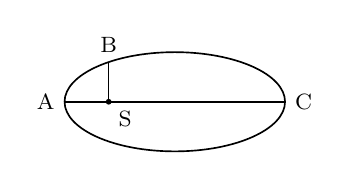
\begin{tikzpicture}[scale=0.7]
\draw (0,0) ellipse (2 and 0.9); \draw (-2,0) -- (2,0); \fill (-1.2,0) circle (1.5pt) node[below right,lbl]{S}; \draw (-1.2,0) -- (-1.2,0.72);
\node[lbl,left] at (-2,0) {A}; \node[lbl,right] at (2,0) {C}; \node[lbl,above] at (-1.2,0.72) {B};
\end{tikzpicture}}\ntag{D}{129}{keph107}{3}{ \textperiodcentered{} Example 7.1}{Class XI Part 1 \textperiodcentered{} Ch 7}}
{\opt{$K_B<K_A<K_C$}{$K_A>K_B>K_C$}{$K_A<K_B<K_C$}{$K_B>K_A>K_C$}}
\topichead{Acceleration due to gravity (g, variation)}{6}
\numoptstrue
\QQ{\qsrc{2025}{32}A body weighs $48\unit{N}$ on the surface of the earth. The gravitational force experienced by the body due to the earth at a height equal to one-third the radius of the earth from its surface is:\ntag{D}{133}{keph107}{7}{ \textperiodcentered{} g(h)=GM/(R+h)\textasciicircum{}2}{Class XI Part 1 \textperiodcentered{} Ch 7}}
{\opt{16\,N}{27\,N}{32\,N}{36\,N}}
\numoptstrue
\QQ{\qsrc{2024}{33}The mass of a planet is $\dfrac1{10}$th that of the earth and its diameter is half that of the earth. The acceleration due to gravity on that planet is:\ntag{A}{133}{keph107}{7}{}{Class XI Part 1 \textperiodcentered{} Ch 7}}
{\opt{$3.92\unit{m\,s^{-2}}$}{$19.6\unit{m\,s^{-2}}$}{$9.8\unit{m\,s^{-2}}$}{$4.9\unit{m\,s^{-2}}$}}
\numoptstrue
\QQ{\qsrc{2020}{143}A body weighs $72\unit{N}$ on the surface of the earth. What is the gravitational force on it, at a height equal to half the radius of the earth?\ntag{D}{143}{keph107}{17}{ \textperiodcentered{} Exercise 7.15}{Class XI Part 1 \textperiodcentered{} Ch 7}}
{\opt{48\,N}{32\,N}{30\,N}{24\,N}}
\numoptstrue
\QQ{\qsrc{2019}{16}A body weighs $200\unit{N}$ on the surface of the earth. How much will it weigh half way down to the centre of the earth?\ntag{D}{143}{keph107}{17}{ \textperiodcentered{} Exercise 7.16}{Class XI Part 1 \textperiodcentered{} Ch 7}}
{\opt{150\,N}{200\,N}{250\,N}{100\,N}}
\numoptstrue
\QQ{\qsrc{2018}{40}If the mass of the Sun were ten times smaller and the universal gravitational constant were ten times larger in magnitude, which of the following is \textit{not} correct?\ntag{A}{133}{keph107}{7}{}{Class XI Part 1 \textperiodcentered{} Ch 7}}
{\opt{Time period of a simple pendulum on the Earth would decrease.}{Walking on the ground would become more difficult.}{Raindrops will fall faster.}{`$g$' on the Earth will not change.}}
\numoptstrue
\QQ{\qsrc{2017}{166}The acceleration due to gravity at a height 1\,km above the earth is the same as at a depth $d$ below the surface of earth. Then:\ntag{D}{133}{keph107}{7}{ \textperiodcentered{} g(h) and g(d)}{Class XI Part 1 \textperiodcentered{} Ch 7}}
{\opt{$d = 1\unit{km}$}{$d = \dfrac32\unit{km}$}{$d = 2\unit{km}$}{$d = \dfrac12\unit{km}$}}
\topichead{Satellites, orbital and escape speed}{6}
\numoptstrue
\QQ{\qsrc{2026}{13}Two planets $P_1$ and $P_2$ with equal mass have radii $R_1$ and $R_2$, respectively, where $R_2 = \dfrac{R_1}{2}$. The escape speeds of $P_1$ and $P_2$ are $v_1$ and $v_2$, respectively. Then $\dfrac{v_2}{v_1}$ is:\ntag{D}{136}{keph107}{10}{ \textperiodcentered{} v=sqrt(2GM/R)}{Class XI Part 1 \textperiodcentered{} Ch 7}}
{\opt{$\dfrac1{\sqrt2}$}{1}{$\sqrt2$}{2}}
\numoptstrue
\QQ{\qsrc{2024}{48}The minimum energy required to launch a satellite of mass $m$ from the surface of earth of mass $M$ and radius $R$ in a circular orbit at an altitude of $2R$ from the surface of the earth is:\ntag{A}{138}{keph107}{12}{}{Class XI Part 1 \textperiodcentered{} Ch 7}}
{\opt{$\dfrac{GmM}{3R}$}{$\dfrac{5GmM}{6R}$}{$\dfrac{2GmM}{3R}$}{$\dfrac{GmM}{2R}$}}
\numoptstrue
\QQ{\qsrc{2023}{43}A satellite is orbiting just above the surface of the earth with period $T$. If $d$ is the density of the earth and $G$ is the universal constant of gravitation, the quantity $\dfrac{3\pi}{Gd}$ represents:\ntag{A}{137}{keph107}{11}{}{Class XI Part 1 \textperiodcentered{} Ch 7}}
{\opt{$\sqrt T$}{$T$}{$T^2$}{$T^3$}}
\numoptstrue
\QQ{\qsrc{2021}{21}The escape velocity from the Earth's surface is $v$. The escape velocity from the surface of another planet having a radius, four times that of Earth and same mass density is:\ntag{A}{136}{keph107}{10}{}{Class XI Part 1 \textperiodcentered{} Ch 7}}
{\opt{$v$}{$2v$}{$3v$}{$4v$}}
\numoptstrue
\QQ{\qsrc{2021}{48}A particle of mass `$m$' is projected with a velocity $v = kV_e$ ($k<1$) from the surface of the earth. ($V_e$ = escape velocity). The maximum height above the surface reached by the particle is:\ntag{A}{136}{keph107}{10}{}{Class XI Part 1 \textperiodcentered{} Ch 7}}
{\opt{$R\left(\dfrac k{1-k}\right)^2$}{$R\left(\dfrac k{1+k}\right)^2$}{$\dfrac{R^2k}{1+k}$}{$\dfrac{Rk^2}{1-k^2}$}}
\numoptstrue
\QQ{\qsrc{2016}{36}The ratio of escape velocity at earth ($v_e$) to the escape velocity at a planet ($v_p$) whose radius and mean density are twice as that of earth is:\ntag{A}{136}{keph107}{10}{ \textperiodcentered{} v\_e=sqrt(2GM/R)}{Class XI Part 1 \textperiodcentered{} Ch 7}}
{\opt{1:2}{$1:2\sqrt2$}{1:4}{$1:\sqrt2$}}
\end{multicols}
\par\needspace{12\baselineskip}\vspace{12pt}
\begin{center}{\pgfornament[width=3.2cm,color=gilt]{87}}\par
{\large\color{navy}\scshape Gravitation \textperiodcentered{} Answer Key}\end{center}
{\small\setlength{\tabcolsep}{1pt}\renewcommand{\arraystretch}{1.5}
\begin{tabularx}{\linewidth}{@{}*{8}{>{\centering\arraybackslash}X}@{}}\toprule
\textbf{1}\,(4) & \textbf{2}\,(3) & \textbf{3}\,(3) & \textbf{4}\,(1) & \textbf{5}\,(1) & \textbf{6}\,(2) & \textbf{7}\,(1) & \textbf{8}\,(2)\\
\textbf{9}\,(2) & \textbf{10}\,(1) & \textbf{11}\,(2) & \textbf{12}\,(4) & \textbf{13}\,(4) & \textbf{14}\,(3) & \textbf{15}\,(3) & \textbf{16}\,(2)\\
\textbf{17}\,(3) & \textbf{18}\,(4) & \textbf{19}\,(4) & \textbf{20}\,(2) &  &  &  & \\\bottomrule\end{tabularx}}\par\smallskip
{\footnotesize Answers of 2021, 2022, 2023, 2025 and 2026 are from the official NTA final keys (checked by the editor); answers of 2016--2020 and 2024 were solved by the editor.
}\par
\par\needspace{18\baselineskip}\vspace{14pt}
\begin{center}{\pgfornament[width=3.2cm,color=gilt]{87}}\par
{\large\color{navy}\scshape Chapter Summary \textperiodcentered{} Gravitation}\end{center}
{\small\setlength{\tabcolsep}{3.5pt}
\begin{tabular*}{\linewidth}{@{\extracolsep{\fill}}l*{11}{c}c@{}}\toprule
Year & 2016 & 2017 & 2018 & 2019 & 2020 & 2021 & 2022 & 2023 & 2024 & 2025 & 2026 & Total\\\midrule
Questions & 2 & 2 & 2 & 2 & 1 & 2 & 1 & 2 & 2 & 2 & 2 & \textbf{20}\\\bottomrule\end{tabular*}}\par\medskip
{\small\textbf{\color{crimson}Topic-wise} (in textbook order)\par\smallskip
\begin{tabularx}{\linewidth}{@{}>{\raggedright\arraybackslash}Xrrrl@{}}\toprule
Topic & Qs & Direct & Years & 2016 $\rightarrow$ 2026\\\midrule
Gravitation (force, field, energy) & \textbf{5} & 1 & 5 & {\scriptsize \textbf{16} \textbf{17} {\color{gray!45}18} \textbf{19} {\color{gray!45}20} {\color{gray!45}21} \textbf{22} \textbf{23} {\color{gray!45}24} {\color{gray!45}25} {\color{gray!45}26}}\\
Kepler's laws and planetary motion & \textbf{3} & 3 & 3 & {\scriptsize {\color{gray!45}16} {\color{gray!45}17} \textbf{18} {\color{gray!45}19} {\color{gray!45}20} {\color{gray!45}21} {\color{gray!45}22} {\color{gray!45}23} {\color{gray!45}24} \textbf{25} \textbf{26}}\\
Acceleration due to gravity (g, variation) & \textbf{6} & 4 & 6 & {\scriptsize {\color{gray!45}16} \textbf{17} \textbf{18} \textbf{19} \textbf{20} {\color{gray!45}21} {\color{gray!45}22} {\color{gray!45}23} \textbf{24} \textbf{25} {\color{gray!45}26}}\\
Satellites, orbital and escape speed & \textbf{6} & 1 & 5 & {\scriptsize \textbf{16} {\color{gray!45}17} {\color{gray!45}18} {\color{gray!45}19} {\color{gray!45}20} \textbf{21} {\color{gray!45}22} \textbf{23} \textbf{24} {\color{gray!45}25} \textbf{26}}\\
\bottomrule\end{tabularx}}\par\medskip
\begin{minipage}[t]{0.34\linewidth}{\small\textbf{\color{crimson}Direct vs Applied}\par\smallskip
\begin{tabular}{@{}lrr@{}}\toprule
Direct from NCERT & \textbf{9} & 45\%\\
\quad text, table, figure & 6 &\\
\quad solved Example & 1 &\\
\quad Exercise & 2 &\\
Applied & \textbf{11} & 55\%\\\midrule
Easy / Mod. / Hard & \multicolumn{2}{r}{12 / 8 / 0}\\\bottomrule
\end{tabular}}\end{minipage}\hfill
\begin{minipage}[t]{0.63\linewidth}{\small\textbf{\color{crimson}What to focus on}\par\smallskip
\begin{itemize}[leftmargin=1.1em,itemsep=1pt,topsep=0pt]
\item 20 questions in 11 papers, about 1.8 per paper; rank 8 of 28 chapters by number of questions.
\item Most asked topic: \textbf{Acceleration due to gravity (g, variation)} (6 questions, in 6 of the 11 years).
\item 3 questions are NCERT solved Examples or Exercises: Example 7.1 (Q 8), Exercise 7.15 (Q 11), Exercise 7.16 (Q 12). Work these by hand.
\item NCERT pages that gave three or more questions: page 136 (5 questions), page 129 (4 questions), page 133 (4 questions), page 134 (3 questions). Read these pages line by line.
\item Difficulty: 12 easy, 8 moderate, 0 hard.
\item 11 applied questions: practise these after the NCERT Examples and Exercises of the chapter.
\end{itemize}}\end{minipage}\par
\chapterpaper{Class XI \textperiodcentered{} Chapter 8}{Mechanical Properties of Solids}{8 questions \textperiodcentered{} 1 topics \textperiodcentered{} NEET 2016--2026}{ckeph201}{XI.8 Mechanical Properties of Solids}
\begin{multicols}{2}
\topichead{Elasticity (Young's modulus)}{8}
\numoptstrue
\QQ{\qsrc{2024}{34}The maximum elongation of a steel wire of $1\unit{m}$ length if the elastic limit of steel and its Young's modulus, respectively, are $8\times10^8\unit{N\,m^{-2}}$ and $2\times10^{11}\unit{N\,m^{-2}}$, is:\ntag{D}{170}{keph201}{4}{ \textperiodcentered{} Y=FL/(A dL)}{Class XI Part 2 \textperiodcentered{} Ch 8}}
{\opt{8\,mm}{4\,mm}{0.4\,mm}{40\,mm}}
\numoptstrue
\QQ{\qsrc{2023}{10}Let a wire be suspended from the ceiling (rigid support) and stretched by a weight $W$ attached at its free end. The longitudinal stress at any point of cross-sectional area $A$ of the wire is:\ntag{D}{168}{keph201}{2}{ \textperiodcentered{} stress=F/A}{Class XI Part 2 \textperiodcentered{} Ch 8}}
{\opt{Zero}{$2W/A$}{$W/A$}{$W/2A$}}
\numoptstrue
\QQ{\qsrc{2022}{43}Given below are two statements: One is labelled as \textbf{Assertion (A)} and the other is labelled as \textbf{Reason (R)}.\par
\textbf{Assertion (A)}: The stretching of a spring is determined by the shear modulus of the material of the spring.\par
\textbf{Reason (R)}: A coil spring of copper has more tensile strength than a steel spring of same dimensions.\par
In the light of the above statements, choose the most appropriate answer from the options given below:\ntag{A}{172}{keph201}{6}{}{Class XI Part 2 \textperiodcentered{} Ch 8}}
{\opt{(A) is false but (R) is true}{Both (A) and (R) are true and (R) is the correct explanation of (A)}{Both (A) and (R) are true and (R) is not the correct explanation of (A)}{(A) is true but (R) is false}}
\numoptstrue
\QQ{\qsrc{2020}{161}A wire of length $L$, area of cross section $A$ is hanging from a fixed support. The length of the wire changes to $L_1$ when mass $M$ is suspended from its free end. The expression for Young's modulus is:\ntag{D}{170}{keph201}{4}{ \textperiodcentered{} Y=FL/(A dL)}{Class XI Part 2 \textperiodcentered{} Ch 8}}
{\opt{$\dfrac{MgL_1}{AL}$}{$\dfrac{Mg(L_1-L)}{AL}$}{$\dfrac{MgL}{AL_1}$}{$\dfrac{MgL}{A(L_1-L)}$}}
\numoptstrue
\QQ{\qsrc{2020}{167}Dimensions of stress are:\ntag{D}{168}{keph201}{2}{ \textperiodcentered{} stress unit}{Class XI Part 2 \textperiodcentered{} Ch 8}}
{\opt{$[\mathrm{MLT^{-2}}]$}{$[\mathrm{ML^2T^{-2}}]$}{$[\mathrm{ML^0T^{-2}}]$}{$[\mathrm{ML^{-1}T^{-2}}]$}}
\numoptstrue
\QQ{\qsrc{2019}{1}When a block of mass $M$ is suspended by a long wire of length $L$, the length of the wire becomes $(L+l)$. The elastic potential energy stored in the extended wire is:\ntag{D}{174}{keph201}{8}{ \textperiodcentered{} elastic PE = (1/2) F x extension}{Class XI Part 2 \textperiodcentered{} Ch 8}}
{\opt{$Mgl$}{$MgL$}{$\dfrac12Mgl$}{$\dfrac12MgL$}}
\numoptstrue
\QQ{\qsrc{2018}{44}Two wires are made of the same material and have the same volume. The first wire has cross-sectional area A and the second wire has cross-sectional area 3A. If the length of the first wire is increased by $\Delta l$ on applying a force F, how much force is needed to stretch the second wire by the same amount?\ntag{A}{170}{keph201}{4}{}{Class XI Part 2 \textperiodcentered{} Ch 8}}
{\opt{4F}{6F}{9F}{F}}
\numoptstrue
\QQ{\qsrc{2017}{164}The bulk modulus of a spherical object is `$B$'. If it is subjected to uniform pressure `$p$', the fractional decrease in radius is:\ntag{A}{173}{keph201}{7}{ \textperiodcentered{} bulk modulus}{Class XI Part 2 \textperiodcentered{} Ch 8}}
{\opt{$\dfrac B{3p}$}{$\dfrac{3p}B$}{$\dfrac p{3B}$}{$\dfrac pB$}}
\end{multicols}
\par\needspace{12\baselineskip}\vspace{12pt}
\begin{center}{\pgfornament[width=3.2cm,color=gilt]{87}}\par
{\large\color{navy}\scshape Mechanical Properties of Solids \textperiodcentered{} Answer Key}\end{center}
{\small\setlength{\tabcolsep}{1pt}\renewcommand{\arraystretch}{1.5}
\begin{tabularx}{\linewidth}{@{}*{8}{>{\centering\arraybackslash}X}@{}}\toprule
\textbf{1}\,(2) & \textbf{2}\,(3) & \textbf{3}\,(4) & \textbf{4}\,(4) & \textbf{5}\,(4) & \textbf{6}\,(3) & \textbf{7}\,(3) & \textbf{8}\,(3)\\\bottomrule\end{tabularx}}\par\smallskip
{\footnotesize Answers of 2021, 2022, 2023, 2025 and 2026 are from the official NTA final keys (checked by the editor); answers of 2016--2020 and 2024 were solved by the editor.
}\par
\par\needspace{18\baselineskip}\vspace{14pt}
\begin{center}{\pgfornament[width=3.2cm,color=gilt]{87}}\par
{\large\color{navy}\scshape Chapter Summary \textperiodcentered{} Mechanical Properties of Solids}\end{center}
{\small\setlength{\tabcolsep}{3.5pt}
\begin{tabular*}{\linewidth}{@{\extracolsep{\fill}}l*{11}{c}c@{}}\toprule
Year & 2016 & 2017 & 2018 & 2019 & 2020 & 2021 & 2022 & 2023 & 2024 & 2025 & 2026 & Total\\\midrule
Questions & 0 & 1 & 1 & 1 & 2 & 0 & 1 & 1 & 1 & 0 & 0 & \textbf{8}\\\bottomrule\end{tabular*}}\par\medskip
{\small\textbf{\color{crimson}Topic-wise} (in textbook order)\par\smallskip
\begin{tabularx}{\linewidth}{@{}>{\raggedright\arraybackslash}Xrrrl@{}}\toprule
Topic & Qs & Direct & Years & 2016 $\rightarrow$ 2026\\\midrule
Elasticity (Young's modulus) & \textbf{8} & 5 & 7 & {\scriptsize {\color{gray!45}16} \textbf{17} \textbf{18} \textbf{19} \textbf{20} {\color{gray!45}21} \textbf{22} \textbf{23} \textbf{24} {\color{gray!45}25} {\color{gray!45}26}}\\
\bottomrule\end{tabularx}}\par\medskip
\begin{minipage}[t]{0.34\linewidth}{\small\textbf{\color{crimson}Direct vs Applied}\par\smallskip
\begin{tabular}{@{}lrr@{}}\toprule
Direct from NCERT & \textbf{5} & 62\%\\
\quad text, table, figure & 5 &\\
\quad solved Example & 0 &\\
\quad Exercise & 0 &\\
Applied & \textbf{3} & 38\%\\\midrule
Easy / Mod. / Hard & \multicolumn{2}{r}{6 / 2 / 0}\\\bottomrule
\end{tabular}}\end{minipage}\hfill
\begin{minipage}[t]{0.63\linewidth}{\small\textbf{\color{crimson}What to focus on}\par\smallskip
\begin{itemize}[leftmargin=1.1em,itemsep=1pt,topsep=0pt]
\item 8 questions in 11 papers, about 0.7 per paper; rank 26 of 28 chapters by number of questions.
\item Most asked topic: \textbf{Elasticity (Young's modulus)} (8 questions, in 7 of the 11 years).
\item NCERT pages that gave three or more questions: page 170 (3 questions). Read these pages line by line.
\item Difficulty: 6 easy, 2 moderate, 0 hard.
\item 3 applied questions: practise these after the NCERT Examples and Exercises of the chapter.
\end{itemize}}\end{minipage}\par
\chapterpaper{Class XI \textperiodcentered{} Chapter 9}{Mechanical Properties of Fluids}{15 questions \textperiodcentered{} 4 topics \textperiodcentered{} NEET 2016--2026}{ckeph202}{XI.9 Mechanical Properties of Fluids}
\begin{multicols}{2}
\topichead{Pressure, Pascal's law and hydrostatics}{2}
\numoptstrue
\QQ{\qsrc{2017}{176}A U tube with both ends open to the atmosphere, is partially filled with water. Oil, which is immiscible with water, is poured into one side until it stands at a distance of $10\unit{mm}$ above the water level on the other side. Meanwhile the water rises by $65\unit{mm}$ from its original level (see diagram). The density of the oil is:
\fig{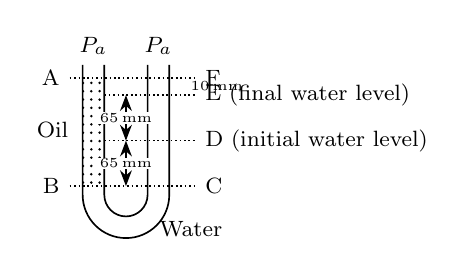
\begin{tikzpicture}[scale=0.55]
\draw (0,4) -- (0,1) arc (180:360:1) -- (2,4); \draw (0.5,4) -- (0.5,1) arc (180:360:0.5) -- (1.5,4);
\fill[pattern=dots] (0,1.2) rectangle (0.5,3.7); \node[lbl,above] at (0.25,4) {$P_a$}; \node[lbl,above] at (1.75,4) {$P_a$};
\draw[densely dotted] (-0.3,3.7) node[left,lbl]{A} -- (2.6,3.7) node[right,lbl]{F}; \draw[densely dotted] (0.5,3.3) -- (2.6,3.3) node[right,lbl]{E (final water level)};
\draw[densely dotted] (0.5,2.25) -- (2.6,2.25) node[right,lbl]{D (initial water level)}; \draw[densely dotted] (-0.3,1.2) node[left,lbl]{B} -- (2.6,1.2) node[right,lbl]{C};
\draw[<->] (1.0,2.25) -- (1.0,3.3) node[midway,fill=white,inner sep=0.5pt,font=\tiny]{65\,mm}; \draw[<->] (1.0,1.2) -- (1.0,2.25) node[midway,fill=white,inner sep=0.5pt,font=\tiny]{65\,mm};
\node[lbl,left] at (-0.1,2.5) {Oil}; \node[lbl] at (2.5,0.2) {Water}; \node[font=\tiny] at (3.1,3.5) {10\,mm};
\end{tikzpicture}}\ntag{A}{184}{keph202}{5}{ \textperiodcentered{} equal pressure at the same level}{Class XI Part 2 \textperiodcentered{} Ch 9}}
{\opt{$425\unit{kg\,m^{-3}}$}{$800\unit{kg\,m^{-3}}$}{$928\unit{kg\,m^{-3}}$}{$650\unit{kg\,m^{-3}}$}}
\numoptstrue
\QQ{\qsrc{2016}{33}Two non-mixing liquids of densities $\rho$ and $n\rho$ ($n>1$) are put in a container. The height of each liquid is $h$. A solid cylinder of length $L$ and density $d$ is put in this container. The cylinder floats with its axis vertical and length $pL$ ($p<1$) in the denser liquid. The density $d$ is equal to:\ntag{A}{184}{keph202}{5}{ \textperiodcentered{} upthrust from both liquids}{Class XI Part 2 \textperiodcentered{} Ch 9}}
{\opt{$\{1+(n+1)p\}\rho$}{$\{2+(n+1)p\}\rho$}{$\{2+(n-1)p\}\rho$}{$\{1+(n-1)p\}\rho$}}
\topichead{Bernoulli's principle and fluid flow}{3}
\numoptstrue
\QQ{\qsrc{2026}{10}Water flows in a streamline motion through a horizontal pipe of circular cross-section as shown in the figure. The pressure difference of water between P and Q is $15\unit{N\,m^{-2}}$. The area of cross-section at P and Q are $40\unit{cm^2}$ and $20\unit{cm^2}$, respectively. The rate of flow of water through the pipe, in $\mathrm{cm^3\,s^{-1}}$, is: [Take density of water $= 1000\unit{kg\,m^{-3}}$]
\fig{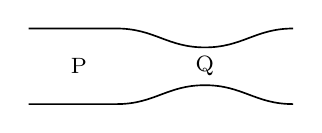
\begin{tikzpicture}[scale=0.8]
\draw (0,0.6) -- (1.4,0.6) .. controls (2.0,0.6) and (2.2,0.3) .. (2.8,0.3) .. controls (3.4,0.3) and (3.6,0.6) .. (4.2,0.6);
\draw (0,-0.6) -- (1.4,-0.6) .. controls (2.0,-0.6) and (2.2,-0.3) .. (2.8,-0.3) .. controls (3.4,-0.3) and (3.6,-0.6) .. (4.2,-0.6);
\node[lbl] at (0.8,0) {P}; \node[lbl] at (2.8,0) {Q};
\end{tikzpicture}}\ntag{A}{188}{keph202}{9}{}{Class XI Part 2 \textperiodcentered{} Ch 9}}
{\opt{100}{200}{300}{400}}
\numoptstrue
\QQ{\qsrc{2023}{34}The venturi-meter works on:\ntag{A}{188}{keph202}{9}{ \textperiodcentered{} venturimeter (Bernoulli)}{Class XI Part 2 \textperiodcentered{} Ch 9}}
{\opt{The principle of perpendicular axes}{Huygen's principle}{Bernoulli's principle}{The principle of parallel axes}}
\numoptstrue
\QQ{\qsrc{2019}{38}A small hole of area of cross-section $2\unit{mm^2}$ is present near the bottom of a fully filled open tank of height $2\unit{m}$. Taking $g = 10\unit{m/s^2}$, the rate of flow of water through the open hole would be nearly:\ntag{D}{189}{keph202}{10}{ \textperiodcentered{} v=sqrt(2gh)}{Class XI Part 2 \textperiodcentered{} Ch 9}}
{\opt{$12.6\times10^{-6}\unit{m^3/s}$}{$8.9\times10^{-6}\unit{m^3/s}$}{$2.23\times10^{-6}\unit{m^3/s}$}{$6.4\times10^{-6}\unit{m^3/s}$}}
\topichead{Viscosity and Stokes' law}{4}
\numoptstrue
\QQ{\qsrc{2026}{12}In the measurement of viscosity of liquids using terminal velocity experiment, spherical balls of same radius but having different densities are used. The variation of the terminal velocity ($v$) with the ratio of density of spherical ball ($\sigma$) to density of the liquid ($\rho$), is best represented by:\ntag{D}{192}{keph202}{13}{ \textperiodcentered{} vt=2a\textasciicircum{}2(rho-sigma)g/9eta}{Class XI Part 2 \textperiodcentered{} Ch 9}}
{\optfig{\gaxes{$\sigma/\rho$}{$v$}{\draw (0.7,0) -- (1.8,1.2); \node[font=\tiny,below] at (0.7,0) {1}; \node[font=\tiny,below] at (0,0) {0};}}
{\gaxes{$\sigma/\rho$}{$v$}{\draw[densely dashed] (0,0) -- (0.7,0.45); \draw (0.7,0.45) -- (1.8,1.15); \node[font=\tiny,below] at (0.7,0) {1}; \node[font=\tiny,below] at (0,0) {0};}}
{\gaxes{$\sigma/\rho$}{$v$}{\draw[densely dashed] (0.3,0) -- (0.7,0.35); \draw (0.7,0.35) -- (1.8,1.3); \node[font=\tiny,below] at (0.7,0) {1}; \node[font=\tiny,below] at (0,0) {0};}}
{\gaxes{$\sigma/\rho$}{$v$}{\draw (0.7,0) -- (0.7,1.0) -- (1.8,1.0); \node[font=\tiny,below] at (0.7,0) {1}; \node[font=\tiny,below] at (0,0) {0};}}}
\numoptstrue
\QQ{\qsrc{2022}{21}A spherical ball is dropped in a long column of a highly viscous liquid. The curve in the graph shown, which represents the speed of the ball ($v$) as a function of time ($t$) is:
\fig{\scalebox{1.5}{\gaxes{$t$}{$v$}{\draw (0,0) -- (1.6,1.5) node[pos=0.1,above left,lbl]{A}; \draw (0,0) .. controls (0.3,0.9) and (0.7,1.2) .. (1.1,1.25) -- (1.9,1.25); \node[lbl] at (0.15,0.95) {B}; \draw (0.25,1.7) .. controls (0.6,0.8) and (1.0,0.5) .. (1.8,0.35); \node[lbl] at (0.35,1.75) {C}; \draw (0.6,1.65) .. controls (1.2,1.55) and (1.5,1.0) .. (1.6,0.5) node[right,lbl]{D};}}}\ntag{D}{192}{keph202}{13}{ \textperiodcentered{} terminal velocity}{Class XI Part 2 \textperiodcentered{} Ch 9}}
{\opt{D}{A}{B}{C}}
\numoptstrue
\QQ{\qsrc{2021}{12}The velocity of a small ball of mass $M$ and density $d$, when dropped in a container filled with glycerine becomes constant after some time. If the density of glycerine is $\dfrac d2$, then the viscous force acting on the ball will be:\ntag{A}{192}{keph202}{13}{}{Class XI Part 2 \textperiodcentered{} Ch 9}}
{\opt{$\dfrac{Mg}2$}{$Mg$}{$\dfrac32Mg$}{$2Mg$}}
\numoptstrue
\QQ{\qsrc{2018}{42}A small sphere of radius `$r$' falls from rest in a viscous liquid. As a result, heat is produced due to viscous force. The rate of production of heat when the sphere attains its terminal velocity, is proportional to\ntag{A}{192}{keph202}{13}{}{Class XI Part 2 \textperiodcentered{} Ch 9}}
{\opt{$r^5$}{$r^2$}{$r^3$}{$r^4$}}
\topichead{Surface tension and capillarity}{6}
\numoptstrue
\QQ{\qsrc{2025}{1}Consider a water tank shown in the figure. It has one wall at $x = L$ and can be taken to be very wide in the $z$ direction. When filled with a liquid of surface tension $S$ and density $\rho$, the liquid surface makes angle $\theta_0$ ($\theta_0\ll1$) with the $x$-axis at $x = L$. If $y(x)$ is the height of the surface then the equation for $y(x)$ is: (take $\theta(x) = \sin\theta(x) = \tan\theta(x) = \dfrac{dy}{dx}$, $g$ is the acceleration due to gravity)
\fig{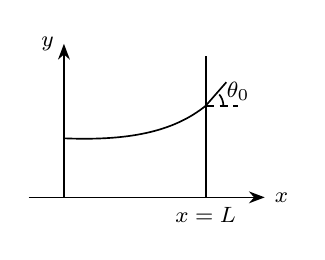
\begin{tikzpicture}[scale=0.75]
\draw[->] (0,0) -- (0,2.6) node[left,lbl]{$y$}; \draw[->] (-0.6,0) -- (3.4,0) node[right,lbl]{$x$};
\draw (2.4,0) -- (2.4,2.4); \node[lbl,below] at (2.4,0) {$x = L$};
\draw (0,1.0) .. controls (1.2,0.95) and (1.9,1.15) .. (2.4,1.55) -- (2.75,1.95);
\draw[densely dashed] (2.4,1.55) -- (2.95,1.55); \draw (2.7,1.55) arc (0:40:0.3); \node[lbl] at (2.95,1.8) {$\theta_0$};
\end{tikzpicture}}\ntag{A}{196}{keph202}{17}{}{Class XI Part 2 \textperiodcentered{} Ch 9}}
{\opt{$\dfrac{d^2y}{dx^2} = \dfrac{\rho g}{S}x$}{$\dfrac{d^2y}{dx^2} = \dfrac{\rho g}{S}y$}{$\dfrac{d^2y}{dx^2} = \sqrt{\dfrac{\rho g}{S}}$}{$\dfrac{dy}{dx} = \sqrt{\dfrac{\rho g}{S}}\,x$}}
\numoptstrue
\QQ{\qsrc{2024}{15}A thin flat circular disc of radius $4.5\unit{cm}$ is placed gently over the surface of water. If surface tension of water is $0.07\unit{N\,m^{-1}}$, then the excess force required to take it away from the surface is:\ntag{A}{195}{keph202}{16}{}{Class XI Part 2 \textperiodcentered{} Ch 9}}
{\opt{99\,N}{19.8\,mN}{198\,N}{1.98\,mN}}
\numoptstrue
\QQ{\qsrc{2023}{27}The amount of energy required to form a soap bubble of radius $2\unit{cm}$ from a soap solution is nearly: (surface tension of soap solution $= 0.03\unit{N\,m^{-1}}$)\ntag{A}{194}{keph202}{15}{}{Class XI Part 2 \textperiodcentered{} Ch 9}}
{\opt{$50.1\times10^{-4}\unit{J}$}{$30.16\times10^{-4}\unit{J}$}{$5.06\times10^{-4}\unit{J}$}{$3.01\times10^{-4}\unit{J}$}}
\numoptstrue
\QQ{\qsrc{2022}{18}If a soap bubble expands, the pressure inside the bubble:\ntag{A}{196}{keph202}{17}{}{Class XI Part 2 \textperiodcentered{} Ch 9}}
{\opt{is equal to the atmospheric pressure}{decreases}{increases}{remains the same}}
\numoptstrue
\QQ{\qsrc{2020}{178}A capillary tube of radius $r$ is immersed in water and water rises in it to a height $h$. The mass of the water in the capillary is $5\unit{g}$. Another capillary tube of radius $2r$ is immersed in water. The mass of water that will rise in this tube is:\ntag{A}{196}{keph202}{17}{}{Class XI Part 2 \textperiodcentered{} Ch 9}}
{\opt{2.5\,g}{5.0\,g}{10.0\,g}{20.0\,g}}
\numoptstrue
\QQ{\qsrc{2019}{7}A soap bubble, having radius of $1\unit{mm}$, is blown from a detergent solution having a surface tension of $2.5\times10^{-2}\unit{N/m}$. The pressure inside the bubble equals at a point $Z_0$ below the free surface of water in a container. Taking $g = 10\unit{m/s^2}$, density of water $= 10^3\unit{kg/m^3}$, the value of $Z_0$ is:\ntag{A}{196}{keph202}{17}{}{Class XI Part 2 \textperiodcentered{} Ch 9}}
{\opt{100\,cm}{10\,cm}{1\,cm}{0.5\,cm}}
\end{multicols}
\par\needspace{12\baselineskip}\vspace{12pt}
\begin{center}{\pgfornament[width=3.2cm,color=gilt]{87}}\par
{\large\color{navy}\scshape Mechanical Properties of Fluids \textperiodcentered{} Answer Key}\end{center}
{\small\setlength{\tabcolsep}{1pt}\renewcommand{\arraystretch}{1.5}
\begin{tabularx}{\linewidth}{@{}*{8}{>{\centering\arraybackslash}X}@{}}\toprule
\textbf{1}\,(3) & \textbf{2}\,(4) & \textbf{3}\,(4) & \textbf{4}\,(3) & \textbf{5}\,(1) & \textbf{6}\,(1) & \textbf{7}\,(3) & \textbf{8}\,(1)\\
\textbf{9}\,(1) & \textbf{10}\,(2) & \textbf{11}\,(2) & \textbf{12}\,(4) & \textbf{13}\,(2) & \textbf{14}\,(3) & \textbf{15}\,(3) & \\\bottomrule\end{tabularx}}\par\smallskip
{\footnotesize Answers of 2021, 2022, 2023, 2025 and 2026 are from the official NTA final keys (checked by the editor); answers of 2016--2020 and 2024 were solved by the editor.
}\par
\par\needspace{18\baselineskip}\vspace{14pt}
\begin{center}{\pgfornament[width=3.2cm,color=gilt]{87}}\par
{\large\color{navy}\scshape Chapter Summary \textperiodcentered{} Mechanical Properties of Fluids}\end{center}
{\small\setlength{\tabcolsep}{3.5pt}
\begin{tabular*}{\linewidth}{@{\extracolsep{\fill}}l*{11}{c}c@{}}\toprule
Year & 2016 & 2017 & 2018 & 2019 & 2020 & 2021 & 2022 & 2023 & 2024 & 2025 & 2026 & Total\\\midrule
Questions & 1 & 1 & 1 & 2 & 1 & 1 & 2 & 2 & 1 & 1 & 2 & \textbf{15}\\\bottomrule\end{tabular*}}\par\medskip
{\small\textbf{\color{crimson}Topic-wise} (in textbook order)\par\smallskip
\begin{tabularx}{\linewidth}{@{}>{\raggedright\arraybackslash}Xrrrl@{}}\toprule
Topic & Qs & Direct & Years & 2016 $\rightarrow$ 2026\\\midrule
Pressure, Pascal's law and hydrostatics & \textbf{2} & 0 & 2 & {\scriptsize \textbf{16} \textbf{17} {\color{gray!45}18} {\color{gray!45}19} {\color{gray!45}20} {\color{gray!45}21} {\color{gray!45}22} {\color{gray!45}23} {\color{gray!45}24} {\color{gray!45}25} {\color{gray!45}26}}\\
Bernoulli's principle and fluid flow & \textbf{3} & 1 & 3 & {\scriptsize {\color{gray!45}16} {\color{gray!45}17} {\color{gray!45}18} \textbf{19} {\color{gray!45}20} {\color{gray!45}21} {\color{gray!45}22} \textbf{23} {\color{gray!45}24} {\color{gray!45}25} \textbf{26}}\\
Viscosity and Stokes' law & \textbf{4} & 2 & 4 & {\scriptsize {\color{gray!45}16} {\color{gray!45}17} \textbf{18} {\color{gray!45}19} {\color{gray!45}20} \textbf{21} \textbf{22} {\color{gray!45}23} {\color{gray!45}24} {\color{gray!45}25} \textbf{26}}\\
Surface tension and capillarity & \textbf{6} & 0 & 6 & {\scriptsize {\color{gray!45}16} {\color{gray!45}17} {\color{gray!45}18} \textbf{19} \textbf{20} {\color{gray!45}21} \textbf{22} \textbf{23} \textbf{24} \textbf{25} {\color{gray!45}26}}\\
\bottomrule\end{tabularx}}\par\medskip
\begin{minipage}[t]{0.34\linewidth}{\small\textbf{\color{crimson}Direct vs Applied}\par\smallskip
\begin{tabular}{@{}lrr@{}}\toprule
Direct from NCERT & \textbf{3} & 20\%\\
\quad text, table, figure & 3 &\\
\quad solved Example & 0 &\\
\quad Exercise & 0 &\\
Applied & \textbf{12} & 80\%\\\midrule
Easy / Mod. / Hard & \multicolumn{2}{r}{5 / 9 / 1}\\\bottomrule
\end{tabular}}\end{minipage}\hfill
\begin{minipage}[t]{0.63\linewidth}{\small\textbf{\color{crimson}What to focus on}\par\smallskip
\begin{itemize}[leftmargin=1.1em,itemsep=1pt,topsep=0pt]
\item 15 questions in 11 papers, about 1.4 per paper; rank 15 of 28 chapters by number of questions.
\item Most asked topic: \textbf{Surface tension and capillarity} (6 questions, in 6 of the 11 years).
\item NCERT pages that gave three or more questions: page 192 (4 questions), page 196 (4 questions). Read these pages line by line.
\item Difficulty: 5 easy, 9 moderate, 1 hard (hard: Q 10).
\item 12 applied questions: practise these after the NCERT Examples and Exercises of the chapter.
\end{itemize}}\end{minipage}\par
\chapterpaper{Class XI \textperiodcentered{} Chapter 10}{Thermal Properties of Matter}{13 questions \textperiodcentered{} 3 topics \textperiodcentered{} NEET 2016--2026}{ckeph203}{XI.10 Thermal Properties of Matter}
\begin{multicols}{2}
\topichead{Thermal expansion}{4}
\numoptstrue
\QQ{\qsrc{2026}{24}The temperature of a metallic sphere of radius $R$ is increased by a small amount $\Delta T$. If the linear coefficient of thermal expansion of the metal is $\alpha$, the approximate increase in the volume of the sphere is:\ntag{D}{207}{keph203}{6}{ \textperiodcentered{} alpha\_V=3 alpha\_l}{Class XI Part 2 \textperiodcentered{} Ch 10}}
{\opt{$2\pi R^3\alpha\Delta T$}{$3\pi R^3\alpha\Delta T$}{$4\pi R^3\alpha\Delta T$}{$6\pi R^3\alpha\Delta T$}}
\numoptstrue
\QQ{\qsrc{2024}{43}A metallic bar of Young's modulus, $0.5\times10^{11}\unit{N\,m^{-2}}$ and coefficient of linear thermal expansion $10^{-5}\,{}^\circ\mathrm C^{-1}$, length $1\unit{m}$ and area of cross-section $10^{-3}\unit{m^2}$ is heated from $0^\circ$C to $100^\circ$C without expansion or bending. The compressive force developed in it is:\ntag{D}{207}{keph203}{6}{ \textperiodcentered{} thermal stress}{Class XI Part 2 \textperiodcentered{} Ch 10}}
{\opt{$2\times10^3\unit{N}$}{$5\times10^3\unit{N}$}{$50\times10^3\unit{N}$}{$100\times10^3\unit{N}$}}
\numoptstrue
\QQ{\qsrc{2019}{14}A copper rod of $88\unit{cm}$ and an aluminium rod of unknown length have their increase in length independent of increase in temperature. The length of aluminium rod is: ($\alpha_{Cu} = 1.7\times10^{-5}\unit{K^{-1}}$ and $\alpha_{Al} = 2.2\times10^{-5}\unit{K^{-1}}$)\ntag{A}{205}{keph203}{4}{}{Class XI Part 2 \textperiodcentered{} Ch 10}}
{\opt{6.8\,cm}{113.9\,cm}{88\,cm}{68\,cm}}
\numoptstrue
\QQ{\qsrc{2016}{16}Coefficient of linear expansion of brass and steel rods are $\alpha_1$ and $\alpha_2$. Lengths of brass and steel rods are $l_1$ and $l_2$ respectively. If $(l_2-l_1)$ is maintained same at all temperatures, which one of the following relations holds good?\ntag{A}{207}{keph203}{6}{ \textperiodcentered{} linear expansion}{Class XI Part 2 \textperiodcentered{} Ch 10}}
{\opt{$\alpha_1l_2 = \alpha_2l_1$}{$\alpha_1l_2^2 = \alpha_2l_1^2$}{$\alpha_1^2l_2 = \alpha_2^2l_1$}{$\alpha_1l_1 = \alpha_2l_2$}}
\topichead{Calorimetry and latent heat}{2}
\numoptstrue
\QQ{\qsrc{2020}{174}The quantities of heat required to raise the temperature of two solid copper spheres of radii $r_1$ and $r_2$ ($r_1 = 1.5r_2$) through 1\,K are in the ratio:\ntag{A}{208}{keph203}{7}{}{Class XI Part 2 \textperiodcentered{} Ch 10}}
{\opt{$\dfrac{27}8$}{$\dfrac94$}{$\dfrac32$}{$\dfrac53$}}
\numoptstrue
\QQ{\qsrc{2016}{35}A piece of ice falls from a height $h$ so that it melts completely. Only one-quarter of the heat produced is absorbed by the ice and all energy of ice gets converted into heat during its fall. The value of $h$ is: [Latent heat of ice is $3.4\times10^5\unit{J/kg}$ and $g = 10\unit{N/kg}$]\ntag{A}{212}{keph203}{11}{ \textperiodcentered{} latent heat}{Class XI Part 2 \textperiodcentered{} Ch 10}}
{\opt{34\,km}{544\,km}{136\,km}{68\,km}}
\topichead{Heat transfer (conduction, radiation, cooling)}{7}
\numoptstrue
\QQ{\qsrc{2025}{19}Three identical heat conducting rods are connected in series as shown in the figure. The rods on the sides have thermal conductivity $2K$ while that in the middle has thermal conductivity $K$. The left end of the combination is maintained at temperature $3T$ and the right end at $T$. The rods are thermally insulated from outside. In steady state, temperature at the left junction is $T_1$ and that at the right junction is $T_2$. The ratio $T_1/T_2$ is
\fig{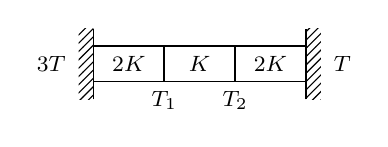
\begin{tikzpicture}[scale=0.75]
\fill[pattern=north east lines] (-0.25,-0.6) rectangle (0,0.6); \fill[pattern=north east lines] (3.6,-0.6) rectangle (3.85,0.6);
\draw (0,-0.6) -- (0,0.6) (3.6,-0.6) -- (3.6,0.6);
\draw (0,-0.3) rectangle (3.6,0.3); \draw (1.2,-0.3) -- (1.2,0.3) (2.4,-0.3) -- (2.4,0.3);
\node[lbl] at (0.6,0) {$2K$}; \node[lbl] at (1.8,0) {$K$}; \node[lbl] at (3.0,0) {$2K$};
\node[lbl,left] at (-0.3,0) {$3T$}; \node[lbl,right] at (3.9,0) {$T$};
\node[lbl,below] at (1.2,-0.3) {$T_1$}; \node[lbl,below] at (2.4,-0.3) {$T_2$};
\end{tikzpicture}}\ntag{A}{215}{keph203}{14}{}{Class XI Part 2 \textperiodcentered{} Ch 10}}
{\opt{$\dfrac32$}{$\dfrac43$}{$\dfrac53$}{$\dfrac54$}}
\numoptstrue
\QQ{\qsrc{2021}{10}A cup of coffee cools from $90^\circ$C to $80^\circ$C in $t$ minutes, when the room temperature is $20^\circ$C. The time taken by a similar cup of coffee to cool from $80^\circ$C to $60^\circ$C at a room temperature same at $20^\circ$C is:\ntag{D}{221}{keph203}{20}{ \textperiodcentered{} Example 10.8}{Class XI Part 2 \textperiodcentered{} Ch 10}}
{\opt{$\dfrac{13}{10}t$}{$\dfrac{13}5t$}{$\dfrac{10}{13}t$}{$\dfrac5{13}t$}}
\numoptstrue
\QQ{\qsrc{2019}{20}The unit of thermal conductivity is:\ntag{D}{214}{keph203}{13}{ \textperiodcentered{} unit of K}{Class XI Part 2 \textperiodcentered{} Ch 10}}
{\opt{$\mathrm{J\,m\,K^{-1}}$}{$\mathrm{J\,m^{-1}K^{-1}}$}{$\mathrm{W\,m\,K^{-1}}$}{$\mathrm{W\,m^{-1}K^{-1}}$}}
\numoptstrue
\QQ{\qsrc{2018}{43}The power radiated by a black body is P and it radiates maximum energy at wavelength, $\lambda_0$. If the temperature of the black body is now changed so that it radiates maximum energy at wavelength $\dfrac34\lambda_0$, the power radiated by it becomes $nP$. The value of $n$ is\ntag{A}{219}{keph203}{18}{}{Class XI Part 2 \textperiodcentered{} Ch 10}}
{\opt{$\dfrac{256}{81}$}{$\dfrac43$}{$\dfrac34$}{$\dfrac{81}{256}$}}
\numoptstrue
\QQ{\qsrc{2017}{146}Two rods A and B of different materials are welded together as shown in figure. Their thermal conductivities are $K_1$ and $K_2$. The thermal conductivity of the composite rod will be:
\fig{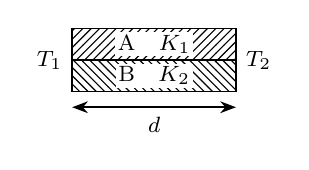
\begin{tikzpicture}[scale=0.8]
\fill[pattern=north east lines] (0,0.5) rectangle (2.6,1); \fill[pattern=north west lines] (0,0) rectangle (2.6,0.5); \draw (0,0) rectangle (2.6,1); \draw (0,0.5) -- (2.6,0.5);
\node[lbl,fill=white,inner sep=1pt] at (1.3,0.75) {A\quad $K_1$}; \node[lbl,fill=white,inner sep=1pt] at (1.3,0.25) {B\quad $K_2$};
\node[lbl,left] at (0,0.5) {$T_1$}; \node[lbl,right] at (2.6,0.5) {$T_2$}; \draw[<->] (0,-0.25) -- (2.6,-0.25) node[midway,below,lbl]{$d$};
\end{tikzpicture}}\ntag{A}{216}{keph203}{15}{ \textperiodcentered{} rods side by side (parallel)}{Class XI Part 2 \textperiodcentered{} Ch 10}}
{\opt{$\dfrac{3(K_1+K_2)}2$}{$K_1+K_2$}{$2(K_1+K_2)$}{$\dfrac{K_1+K_2}2$}}
\numoptstrue
\QQ{\qsrc{2017}{160}A spherical black body with a radius of $12\unit{cm}$ radiates 450 watt power at 500\,K. If the radius were halved and the temperature doubled, the power radiated in watt would be:\ntag{A}{219}{keph203}{18}{ \textperiodcentered{} Stefan-Boltzmann law}{Class XI Part 2 \textperiodcentered{} Ch 10}}
{\opt{450}{1000}{1800}{225}}
\numoptstrue
\QQ{\qsrc{2016}{15}A black body is at a temperature of 5760\,K. The energy of radiation emitted by the body at wavelength 250\,nm is $U_1$, at wavelength 500\,nm is $U_2$ and that at 1000\,nm is $U_3$. Wien's constant, $b = 2.88\times10^6\unit{nm\,K}$. Which of the following is correct?\ntag{A}{218}{keph203}{17}{ \textperiodcentered{} Wien's law}{Class XI Part 2 \textperiodcentered{} Ch 10}}
{\opt{$U_1 = 0$}{$U_3 = 0$}{$U_1>U_2$}{$U_2>U_1$}}
\end{multicols}
\par\needspace{12\baselineskip}\vspace{12pt}
\begin{center}{\pgfornament[width=3.2cm,color=gilt]{87}}\par
{\large\color{navy}\scshape Thermal Properties of Matter \textperiodcentered{} Answer Key}\end{center}
{\small\setlength{\tabcolsep}{1pt}\renewcommand{\arraystretch}{1.5}
\begin{tabularx}{\linewidth}{@{}*{8}{>{\centering\arraybackslash}X}@{}}\toprule
\textbf{1}\,(3) & \textbf{2}\,(3) & \textbf{3}\,(4) & \textbf{4}\,(4) & \textbf{5}\,(1) & \textbf{6}\,(3) & \textbf{7}\,(3) & \textbf{8}\,(2)\\
\textbf{9}\,(4) & \textbf{10}\,(1) & \textbf{11}\,(4) & \textbf{12}\,(3) & \textbf{13}\,(4) &  &  & \\\bottomrule\end{tabularx}}\par\smallskip
{\footnotesize Answers of 2021, 2022, 2023, 2025 and 2026 are from the official NTA final keys (checked by the editor); answers of 2016--2020 and 2024 were solved by the editor.
}\par
\par\needspace{18\baselineskip}\vspace{14pt}
\begin{center}{\pgfornament[width=3.2cm,color=gilt]{87}}\par
{\large\color{navy}\scshape Chapter Summary \textperiodcentered{} Thermal Properties of Matter}\end{center}
{\small\setlength{\tabcolsep}{3.5pt}
\begin{tabular*}{\linewidth}{@{\extracolsep{\fill}}l*{11}{c}c@{}}\toprule
Year & 2016 & 2017 & 2018 & 2019 & 2020 & 2021 & 2022 & 2023 & 2024 & 2025 & 2026 & Total\\\midrule
Questions & 3 & 2 & 1 & 2 & 1 & 1 & 0 & 0 & 1 & 1 & 1 & \textbf{13}\\\bottomrule\end{tabular*}}\par\medskip
{\small\textbf{\color{crimson}Topic-wise} (in textbook order)\par\smallskip
\begin{tabularx}{\linewidth}{@{}>{\raggedright\arraybackslash}Xrrrl@{}}\toprule
Topic & Qs & Direct & Years & 2016 $\rightarrow$ 2026\\\midrule
Thermal expansion & \textbf{4} & 2 & 4 & {\scriptsize \textbf{16} {\color{gray!45}17} {\color{gray!45}18} \textbf{19} {\color{gray!45}20} {\color{gray!45}21} {\color{gray!45}22} {\color{gray!45}23} \textbf{24} {\color{gray!45}25} \textbf{26}}\\
Calorimetry and latent heat & \textbf{2} & 0 & 2 & {\scriptsize \textbf{16} {\color{gray!45}17} {\color{gray!45}18} {\color{gray!45}19} \textbf{20} {\color{gray!45}21} {\color{gray!45}22} {\color{gray!45}23} {\color{gray!45}24} {\color{gray!45}25} {\color{gray!45}26}}\\
Heat transfer (conduction, radiation, cooling) & \textbf{7} & 2 & 6 & {\scriptsize \textbf{16} \textbf{17} \textbf{18} \textbf{19} {\color{gray!45}20} \textbf{21} {\color{gray!45}22} {\color{gray!45}23} {\color{gray!45}24} \textbf{25} {\color{gray!45}26}}\\
\bottomrule\end{tabularx}}\par\medskip
\begin{minipage}[t]{0.34\linewidth}{\small\textbf{\color{crimson}Direct vs Applied}\par\smallskip
\begin{tabular}{@{}lrr@{}}\toprule
Direct from NCERT & \textbf{4} & 31\%\\
\quad text, table, figure & 3 &\\
\quad solved Example & 1 &\\
\quad Exercise & 0 &\\
Applied & \textbf{9} & 69\%\\\midrule
Easy / Mod. / Hard & \multicolumn{2}{r}{6 / 7 / 0}\\\bottomrule
\end{tabular}}\end{minipage}\hfill
\begin{minipage}[t]{0.63\linewidth}{\small\textbf{\color{crimson}What to focus on}\par\smallskip
\begin{itemize}[leftmargin=1.1em,itemsep=1pt,topsep=0pt]
\item 13 questions in 11 papers, about 1.2 per paper; rank 21 of 28 chapters by number of questions.
\item Most asked topic: \textbf{Heat transfer (conduction, radiation, cooling)} (7 questions, in 6 of the 11 years).
\item 1 questions are NCERT solved Examples or Exercises: Example 10.8 (Q 8). Work these by hand.
\item NCERT pages that gave three or more questions: page 207 (3 questions). Read these pages line by line.
\item Difficulty: 6 easy, 7 moderate, 0 hard.
\item 9 applied questions: practise these after the NCERT Examples and Exercises of the chapter.
\end{itemize}}\end{minipage}\par
\chapterpaper{Class XI \textperiodcentered{} Chapter 11}{Thermodynamics}{15 questions \textperiodcentered{} 3 topics \textperiodcentered{} NEET 2016--2026}{ckeph204}{XI.11 Thermodynamics}
\begin{multicols}{2}
\topichead{First law of thermodynamics}{2}
\numoptstrue
\QQ{\qsrc{2025}{41}Two gases A and B are filled at the same pressure in separate cylinders with movable pistons of radius $r_A$ and $r_B$, respectively. On supplying an equal amount of heat to both the systems reversibly under constant pressure, the pistons of gas A and B are displaced by $16\unit{cm}$ and $9\unit{cm}$, respectively. If the change in their internal energy is the same, then the ratio $r_A/r_B$ is equal to\ntag{A}{230}{keph204}{5}{}{Class XI Part 2 \textperiodcentered{} Ch 11}}
{\opt{$\dfrac43$}{$\dfrac34$}{$\dfrac2{\sqrt3}$}{$\dfrac{\sqrt3}2$}}
\numoptstrue
\QQ{\qsrc{2018}{45}A sample of 0.1\,g of water at $100^\circ$C and normal pressure ($1.013\times10^5\unit{N\,m^{-2}}$) requires 54\,cal of heat energy to convert to steam at $100^\circ$C. If the volume of the steam produced is 167.1\,cc, the change in internal energy of the sample, is\ntag{A}{231}{keph204}{6}{}{Class XI Part 2 \textperiodcentered{} Ch 11}}
{\opt{42.2\,J}{208.7\,J}{104.3\,J}{84.5\,J}}
\topichead{Thermodynamic processes}{9}
\numoptstrue
\QQ{\qsrc{2026}{17}In an adiabatic expansion, the temperature of one mole of an ideal monatomic gas ($\gamma = 5/3$) decreases from $60\unit{K}$ to $50\unit{K}$. The work done by the gas in the process is: (Take the universal gas constant as $R = 8.3\unit{J\,mol^{-1}K^{-1}}$)\ntag{D}{235}{keph204}{10}{ \textperiodcentered{} W=muR(T1-T2)/(gamma-1)}{Class XI Part 2 \textperiodcentered{} Ch 11}}
{\opt{41.5\,J}{83\,J}{124.5\,J}{166\,J}}
\numoptstrue
\QQ{\qsrc{2026}{39}One mole of an ideal monatomic gas undergoes a cyclic process as shown in the figure. The total heat supplied to the gas is:
\fig{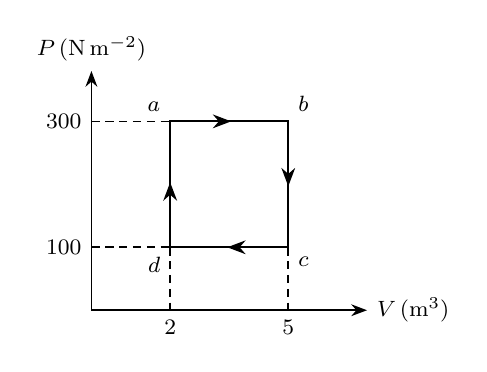
\begin{tikzpicture}[xscale=0.5,yscale=0.008]
\draw[->] (0,0) -- (7,0) node[right,lbl]{$V\,(\mathrm{m^3})$}; \draw[->] (0,0) -- (0,380) node[above,lbl]{$P\,(\mathrm{N\,m^{-2}})$};
\draw[densely dashed] (0,300) node[left,lbl]{300} -- (2,300) (0,100) node[left,lbl]{100} -- (2,100) (2,100) -- (2,0) node[below,lbl]{2} (5,100) -- (5,0) node[below,lbl]{5};
\draw[thick,postaction={decorate},decoration={markings,mark=at position 0.125 with {\arrow{Stealth}},mark=at position 0.375 with {\arrow{Stealth}},mark=at position 0.625 with {\arrow{Stealth}},mark=at position 0.875 with {\arrow{Stealth}}}] (2,300) -- (5,300) -- (5,100) -- (2,100) -- cycle;
\node[lbl,above left] at (2,300) {$a$}; \node[lbl,above right] at (5,300) {$b$}; \node[lbl,below right] at (5,100) {$c$}; \node[lbl,below left] at (2,100) {$d$};
\end{tikzpicture}}\ntag{D}{236}{keph204}{11}{ \textperiodcentered{} cyclic process: Q=W=area}{Class XI Part 2 \textperiodcentered{} Ch 11}}
{\opt{400\,J}{500\,J}{600\,J}{800\,J}}
\numoptstrue
\QQ{\qsrc{2024}{27}A thermodynamic system is taken through the cycle $abcda$. The work done by the gas along the path $bc$ is:
\fig{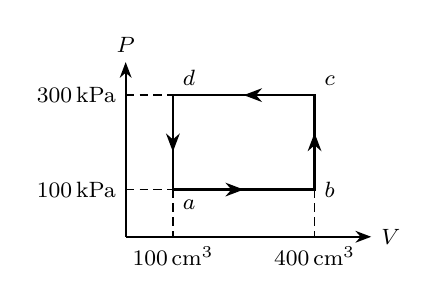
\begin{tikzpicture}[xscale=0.006,yscale=0.006]
\draw[->] (0,0) -- (520,0) node[right,lbl]{$V$}; \draw[->] (0,0) -- (0,370) node[above,lbl]{$P$};
\draw[densely dashed] (0,300) node[left,lbl]{300\,kPa} -- (100,300) (0,100) node[left,lbl]{100\,kPa} -- (100,100) (100,100) -- (100,0) node[below,lbl]{100\,cm$^3$} (400,100) -- (400,0) node[below,lbl]{400\,cm$^3$};
\draw[thick,postaction={decorate},decoration={markings,mark=at position 0.15 with {\arrow{Stealth}},mark=at position 0.42 with {\arrow{Stealth}},mark=at position 0.65 with {\arrow{Stealth}},mark=at position 0.92 with {\arrow{Stealth}}}] (100,100) -- (400,100) -- (400,300) -- (100,300) -- cycle;
\node[lbl,below right] at (100,100) {$a$}; \node[lbl,right] at (400,100) {$b$}; \node[lbl,above right] at (400,300) {$c$}; \node[lbl,above right] at (100,300) {$d$};
\end{tikzpicture}}\ntag{D}{235}{keph204}{10}{ \textperiodcentered{} isochoric: W=0}{Class XI Part 2 \textperiodcentered{} Ch 11}}
{\opt{$-60\unit{J}$}{zero}{30\,J}{$-90\unit{J}$}}
\numoptstrue
\QQ{\qsrc{2022}{12}An ideal gas undergoes four different processes from the same initial state as shown in the figure below. Those processes are adiabatic, isothermal, isobaric and isochoric. The curve which represents the adiabatic process among 1, 2, 3 and 4 is:
\fig{\scalebox{1.5}{\gaxes{$V$}{$P$}{\draw (0.3,1.5) -- (1.8,1.5) node[right,lbl]{4}; \draw (0.3,1.5) -- (0.3,0.2) node[right,lbl]{1}; \draw (0.3,1.5) .. controls (0.8,1.0) and (1.3,0.95) .. (1.8,0.85) node[right,lbl]{3}; \draw (0.3,1.5) .. controls (0.7,0.8) and (1.2,0.7) .. (1.8,0.6) node[right,lbl]{2};}}}\ntag{A}{235}{keph204}{10}{}{Class XI Part 2 \textperiodcentered{} Ch 11}}
{\opt{4}{1}{2}{3}}
\numoptstrue
\QQ{\qsrc{2020}{141}Two cylinders A and B of equal capacity are connected to each other via a stop cock. A contains an ideal gas at standard temperature and pressure. B is completely evacuated. The entire system is thermally insulated. The stop cock is suddenly opened. The process is:\ntag{A}{236}{keph204}{11}{ \textperiodcentered{} free expansion}{Class XI Part 2 \textperiodcentered{} Ch 11}}
{\opt{isothermal}{adiabatic}{isochoric}{isobaric}}
\numoptstrue
\QQ{\qsrc{2019}{40}In which of the following processes, heat is neither absorbed nor released by a system?\ntag{D}{234}{keph204}{9}{ \textperiodcentered{} Table 11.2}{Class XI Part 2 \textperiodcentered{} Ch 11}}
{\opt{isothermal}{adiabatic}{isobaric}{isochoric}}
\numoptstrue
\QQ{\qsrc{2018}{1}The volume ($V$) of a monatomic gas varies with its temperature ($T$), as shown in the graph. The ratio of work done by the gas, to the heat absorbed by it, when it undergoes a change from state A to state B, is
\fig{\gaxes{$T$}{$V$}{\draw (0,0) -- (1.9,0.9); \draw[very thick,->] (0.6,0.28) -- (1.1,0.52); \node[lbl,above] at (0.6,0.28) {A}; \node[lbl,above] at (1.4,0.66) {B}; \node[lbl,below left] at (0,0) {O};}}\ntag{A}{235}{keph204}{10}{}{Class XI Part 2 \textperiodcentered{} Ch 11}}
{\opt{$\dfrac13$}{$\dfrac23$}{$\dfrac25$}{$\dfrac27$}}
\numoptstrue
\QQ{\qsrc{2017}{155}Thermodynamic processes are indicated in the following diagram.
\fig{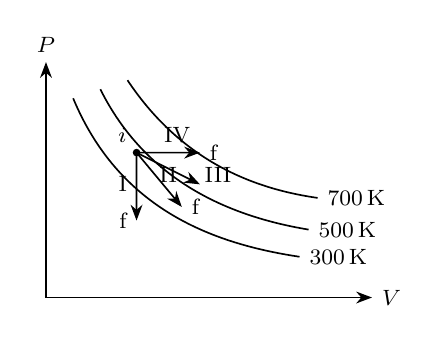
\begin{tikzpicture}[scale=1.15]
\draw[->] (0,0) -- (3.6,0) node[right,lbl]{$V$}; \draw[->] (0,0) -- (0,2.6) node[above,lbl]{$P$};
\draw (0.3,2.2) .. controls (0.8,1.0) and (1.8,0.6) .. (2.8,0.45) node[right,lbl]{300\,K}; \draw (0.6,2.3) .. controls (1.1,1.3) and (2.0,0.9) .. (2.9,0.75) node[right,lbl]{500\,K}; \draw (0.9,2.4) .. controls (1.5,1.5) and (2.3,1.2) .. (3.0,1.1) node[right,lbl]{700\,K};
\coordinate (i) at (1.0,1.6); \fill (i) circle (1.2pt) node[above left,lbl]{$i$};
\draw[->] (i) -- (1.0,0.85) node[left,lbl]{f}; \node[lbl] at (0.85,1.25) {I}; \draw[->] (i) -- (1.5,1.0) node[right,lbl]{f}; \node[lbl] at (1.35,1.35) {II};
\draw[->] (i) -- (1.7,1.6) node[right,lbl]{f}; \node[lbl] at (1.45,1.8) {IV}; \draw[->] (i) -- (1.7,1.25); \node[lbl] at (1.9,1.35) {III};
\end{tikzpicture}}
Match the following:\par\smallskip
\begin{tabular}{@{}ll@{\qquad}ll@{}}
P. & Process I & a. & Adiabatic\\ Q. & Process II & b. & Isobaric\\ R. & Process III & c. & Isochoric\\ S. & Process IV & d. & Isothermal
\end{tabular}\ntag{A}{232}{keph204}{7}{}{Class XI Part 2 \textperiodcentered{} Ch 11}}
{\opt{P$\to$c, Q$\to$a, R$\to$d, S$\to$b}{P$\to$c, Q$\to$d, R$\to$b, S$\to$a}{P$\to$d, Q$\to$b, R$\to$a, S$\to$c}{P$\to$a, Q$\to$c, R$\to$d, S$\to$b}}
\numoptstrue
\QQ{\qsrc{2016}{30}A gas is compressed isothermally to half its initial volume. The same gas is compressed separately through an adiabatic process until its volume is again reduced to half. Then:\ntag{A}{233}{keph204}{8}{ \textperiodcentered{} adiabatic curve is steeper}{Class XI Part 2 \textperiodcentered{} Ch 11}}
{\opt{Compressing the gas isothermally will require more work to be done.}{Compressing the gas through adiabatic process will require more work to be done.}{Compressing the gas isothermally or adiabatically will require the same amount of work.}{Which of the case (whether compression through isothermal or through adiabatic process) requires more work will depend upon the atomicity of the gas.}}
\topichead{Second law and heat engines}{4}
\numoptstrue
\QQ{\qsrc{2023}{26}A Carnot engine has an efficiency of 50\% when its source is at a temperature $327^\circ$C. The temperature of the sink is:\ntag{D}{238}{keph204}{13}{ \textperiodcentered{} eta=1-T2/T1}{Class XI Part 2 \textperiodcentered{} Ch 11}}
{\opt{$200^\circ$C}{$27^\circ$C}{$15^\circ$C}{$100^\circ$C}}
\numoptstrue
\QQ{\qsrc{2018}{4}The efficiency of an ideal heat engine working between the freezing point and boiling point of water, is\ntag{D}{238}{keph204}{13}{ \textperiodcentered{} eta=1-T2/T1}{Class XI Part 2 \textperiodcentered{} Ch 11}}
{\opt{6.25\%}{20\%}{26.8\%}{12.5\%}}
\numoptstrue
\QQ{\qsrc{2017}{180}A carnot engine having an efficiency of $\dfrac1{10}$ as heat engine, is used as a refrigerator. If the work done on the system is 10\,J, the amount of energy absorbed from the reservoir at lower temperature is:\ntag{A}{236}{keph204}{11}{ \textperiodcentered{} refrigerator}{Class XI Part 2 \textperiodcentered{} Ch 11}}
{\opt{90\,J}{99\,J}{100\,J}{1\,J}}
\numoptstrue
\QQ{\qsrc{2016}{11}A refrigerator works between $4^\circ$C and $30^\circ$C. It is required to remove 600 calories of heat every second in order to keep the temperature of the refrigerated space constant. The power required is: (Take 1\,cal $= 4.2$\,Joules)\ntag{A}{236}{keph204}{11}{ \textperiodcentered{} refrigerator}{Class XI Part 2 \textperiodcentered{} Ch 11}}
{\opt{2.365\,W}{23.65\,W}{236.5\,W}{2365\,W}}
\end{multicols}
\par\needspace{12\baselineskip}\vspace{12pt}
\begin{center}{\pgfornament[width=3.2cm,color=gilt]{87}}\par
{\large\color{navy}\scshape Thermodynamics \textperiodcentered{} Answer Key}\end{center}
{\small\setlength{\tabcolsep}{1pt}\renewcommand{\arraystretch}{1.5}
\begin{tabularx}{\linewidth}{@{}*{8}{>{\centering\arraybackslash}X}@{}}\toprule
\textbf{1}\,(2) & \textbf{2}\,(2) & \textbf{3}\,(3) & \textbf{4}\,(3) & \textbf{5}\,(2) & \textbf{6}\,(3) & \textbf{7}\,(2) & \textbf{8}\,(2)\\
\textbf{9}\,(3) & \textbf{10}\,(1) & \textbf{11}\,(2) & \textbf{12}\,(2) & \textbf{13}\,(3) & \textbf{14}\,(1) & \textbf{15}\,(3) & \\\bottomrule\end{tabularx}}\par\smallskip
{\footnotesize Answers of 2021, 2022, 2023, 2025 and 2026 are from the official NTA final keys (checked by the editor); answers of 2016--2020 and 2024 were solved by the editor.
}\par
\par\needspace{18\baselineskip}\vspace{14pt}
\begin{center}{\pgfornament[width=3.2cm,color=gilt]{87}}\par
{\large\color{navy}\scshape Chapter Summary \textperiodcentered{} Thermodynamics}\end{center}
{\small\setlength{\tabcolsep}{3.5pt}
\begin{tabular*}{\linewidth}{@{\extracolsep{\fill}}l*{11}{c}c@{}}\toprule
Year & 2016 & 2017 & 2018 & 2019 & 2020 & 2021 & 2022 & 2023 & 2024 & 2025 & 2026 & Total\\\midrule
Questions & 2 & 2 & 3 & 1 & 1 & 0 & 1 & 1 & 1 & 1 & 2 & \textbf{15}\\\bottomrule\end{tabular*}}\par\medskip
{\small\textbf{\color{crimson}Topic-wise} (in textbook order)\par\smallskip
\begin{tabularx}{\linewidth}{@{}>{\raggedright\arraybackslash}Xrrrl@{}}\toprule
Topic & Qs & Direct & Years & 2016 $\rightarrow$ 2026\\\midrule
First law of thermodynamics & \textbf{2} & 0 & 2 & {\scriptsize {\color{gray!45}16} {\color{gray!45}17} \textbf{18} {\color{gray!45}19} {\color{gray!45}20} {\color{gray!45}21} {\color{gray!45}22} {\color{gray!45}23} {\color{gray!45}24} \textbf{25} {\color{gray!45}26}}\\
Thermodynamic processes & \textbf{9} & 4 & 8 & {\scriptsize \textbf{16} \textbf{17} \textbf{18} \textbf{19} \textbf{20} {\color{gray!45}21} \textbf{22} {\color{gray!45}23} \textbf{24} {\color{gray!45}25} \textbf{26}}\\
Second law and heat engines & \textbf{4} & 2 & 4 & {\scriptsize \textbf{16} \textbf{17} \textbf{18} {\color{gray!45}19} {\color{gray!45}20} {\color{gray!45}21} {\color{gray!45}22} \textbf{23} {\color{gray!45}24} {\color{gray!45}25} {\color{gray!45}26}}\\
\bottomrule\end{tabularx}}\par\medskip
\begin{minipage}[t]{0.34\linewidth}{\small\textbf{\color{crimson}Direct vs Applied}\par\smallskip
\begin{tabular}{@{}lrr@{}}\toprule
Direct from NCERT & \textbf{6} & 40\%\\
\quad text, table, figure & 6 &\\
\quad solved Example & 0 &\\
\quad Exercise & 0 &\\
Applied & \textbf{9} & 60\%\\\midrule
Easy / Mod. / Hard & \multicolumn{2}{r}{7 / 8 / 0}\\\bottomrule
\end{tabular}}\end{minipage}\hfill
\begin{minipage}[t]{0.63\linewidth}{\small\textbf{\color{crimson}What to focus on}\par\smallskip
\begin{itemize}[leftmargin=1.1em,itemsep=1pt,topsep=0pt]
\item 15 questions in 11 papers, about 1.4 per paper; rank 14 of 28 chapters by number of questions.
\item Most asked topic: \textbf{Thermodynamic processes} (9 questions, in 8 of the 11 years).
\item Asked in 8 or more of the 11 years: Thermodynamic processes.
\item NCERT pages that gave three or more questions: page 235 (4 questions), page 236 (4 questions). Read these pages line by line.
\item Difficulty: 7 easy, 8 moderate, 0 hard.
\item 9 applied questions: practise these after the NCERT Examples and Exercises of the chapter.
\end{itemize}}\end{minipage}\par
\chapterpaper{Class XI \textperiodcentered{} Chapter 12}{Kinetic Theory}{15 questions \textperiodcentered{} 1 topics \textperiodcentered{} NEET 2016--2026}{ckeph205}{XI.12 Kinetic Theory}
\begin{multicols}{2}
\topichead{Kinetic theory of gases}{15}
\numoptstrue
\QQ{\qsrc{2026}{2}The mean free path of molecules in an ideal gas A is half that of another ideal gas B. The diameter of the spherical molecules of gas A is twice the diameter of the molecules of B. If number densities of the gases A and B are $n_A$ and $n_B$, respectively, the correct option is:\ntag{D}{254}{keph205}{11}{ \textperiodcentered{} l=1/(sqrt2 n pi d\textasciicircum{}2)}{Class XI Part 2 \textperiodcentered{} Ch 12}}
{\opt{$n_A = n_B$}{$n_A = 2n_B$}{$n_A = \dfrac14n_B$}{$n_A = \dfrac12n_B$}}
\numoptstrue
\QQ{\qsrc{2026}{45}An ideal gas is made of polyatomic molecules. Each of the molecules has three translational, three rotational and $f$ number of vibrational modes. If the ratio of heat capacities $C_P/C_V$ of the gas is $8/7$, then the value of $f$ is:\ntag{D}{253}{keph205}{10}{ \textperiodcentered{} Cv=(3+f)R}{Class XI Part 2 \textperiodcentered{} Ch 12}}
{\opt{4}{3}{2}{1}}
\numoptstrue
\QQ{\qsrc{2025}{14}An oxygen cylinder of volume 30 litre has 18.20 moles of oxygen. After some oxygen is withdrawn from the cylinder, its gauge pressure drops to 11 atmospheric pressure at temperature $27^\circ$C. The mass of the oxygen withdrawn from the cylinder is nearly equal to: [Given, $R = \dfrac{100}{12}\unit{J\,mol^{-1}K^{-1}}$, and molecular mass of $\mathrm O_2 = 32$, $1\unit{atm}$ pressure $= 1.01\times10^5\unit{N/m^2}$]\ntag{A}{246}{keph205}{3}{}{Class XI Part 2 \textperiodcentered{} Ch 12}}
{\opt{0.125\,kg}{0.144\,kg}{0.116\,kg}{0.156\,kg}}
\numoptstrue
\QQ{\qsrc{2025}{29}A container has two chambers of volumes $V_1 = 2$ litres and $V_2 = 3$ litres separated by a partition made of a thermal insulator. The chambers contain $n_1 = 5$ and $n_2 = 4$ moles of ideal gas at pressures $p_1 = 1\unit{atm}$ and $p_2 = 2\unit{atm}$, respectively. When the partition is removed, the mixture attains an equilibrium pressure of:\ntag{A}{247}{keph205}{4}{}{Class XI Part 2 \textperiodcentered{} Ch 12}}
{\opt{1.3\,atm}{1.6\,atm}{1.4\,atm}{1.8\,atm}}
\numoptstrue
\QQ{\qsrc{2024}{49}The following graph represents the T-V curves of an ideal gas (where T is the temperature and V the volume) at three pressures $P_1$, $P_2$ and $P_3$ compared with those of Charles's law represented as dotted lines.
\fig{\gaxes{$V$}{$T$}{\draw (0.15,0.1) .. controls (0.4,0.7) and (0.6,1.2) .. (0.7,1.7) node[above,font=\tiny]{$P_1$}; \draw (0.25,0.1) .. controls (0.6,0.6) and (0.8,1.0) .. (1.0,1.5) node[above,font=\tiny]{$P_2$}; \draw (0.35,0.1) .. controls (0.8,0.45) and (1.1,0.8) .. (1.35,1.2) node[right,font=\tiny]{$P_3$}; \draw[densely dotted] (0,0) -- (0.65,1.7) (0,0) -- (0.95,1.5) (0,0) -- (1.35,1.2);}}
Then the correct relation is:\ntag{A}{246}{keph205}{3}{}{Class XI Part 2 \textperiodcentered{} Ch 12}}
{\opt{$P_1>P_2>P_3$}{$P_3>P_2>P_1$}{$P_1>P_3>P_2$}{$P_2>P_1>P_3$}}
\numoptstrue
\QQ{\qsrc{2023}{12}The temperature of a gas is $-50^\circ$C. To what temperature the gas should be heated so that the rms speed is increased by 3 times?\ntag{A}{250}{keph205}{7}{}{Class XI Part 2 \textperiodcentered{} Ch 12}}
{\opt{223\,K}{$669^\circ$C}{$3295^\circ$C}{3097\,K}}
\numoptstrue
\QQ{\qsrc{2022}{37}The volume occupied by the molecules contained in $4.5\unit{kg}$ water at STP, if the intermolecular forces vanish away is:\ntag{A}{246}{keph205}{3}{}{Class XI Part 2 \textperiodcentered{} Ch 12}}
{\opt{$5.6\unit{m^3}$}{$5.6\times10^6\unit{m^3}$}{$5.6\times10^3\unit{m^3}$}{$5.6\times10^{-3}\unit{m^3}$}}
\numoptstrue
\QQ{\qsrc{2021}{7}Match Column-I and Column-II and choose the correct match from the given choices.\par\smallskip
\begin{tabular}{@{}lp{0.42\linewidth}ll@{}}
\multicolumn{2}{@{}l}{\textit{Column-I}} & \multicolumn{2}{l}{\textit{Column-II}}\\
(A) & Root mean square speed of gas molecules & (P) & $\frac13nm\bar v^2$\\
(B) & Pressure exerted by ideal gas & (Q) & $\sqrt{\frac{3RT}M}$\\
(C) & Average kinetic energy of a molecule & (R) & $\frac52RT$\\
(D) & Total internal energy of 1 mole of a diatomic gas & (S) & $\frac32k_BT$
\end{tabular}\ntag{D}{250}{keph205}{7}{ \textperiodcentered{} vrms, P=(1/3)nm<v\textasciicircum{}2>, (3/2)kBT}{Class XI Part 2 \textperiodcentered{} Ch 12}}
{\opt{(A)-(R), (B)-(P), (C)-(S), (D)-(Q)}{(A)-(Q), (B)-(R), (C)-(S), (D)-(P)}{(A)-(Q), (B)-(P), (C)-(S), (D)-(R)}{(A)-(R), (B)-(Q), (C)-(P), (D)-(S)}}
\numoptstrue
\QQ{\qsrc{2020}{139}A cylinder contains hydrogen gas at pressure of $249\unit{kPa}$ and temperature $27^\circ$C. Its density is: ($R = 8.3\unit{J\,mol^{-1}K^{-1}}$)\ntag{A}{246}{keph205}{3}{}{Class XI Part 2 \textperiodcentered{} Ch 12}}
{\opt{$0.5\unit{kg/m^3}$}{$0.2\unit{kg/m^3}$}{$0.1\unit{kg/m^3}$}{$0.02\unit{kg/m^3}$}}
\numoptstrue
\QQ{\qsrc{2020}{155}The mean free path for a gas, with molecular diameter $d$ and number density $n$ can be expressed as:\ntag{D}{254}{keph205}{11}{ \textperiodcentered{} l=1/(sqrt2 n pi d\textasciicircum{}2)}{Class XI Part 2 \textperiodcentered{} Ch 12}}
{\opt{$\dfrac1{\sqrt2\,n\pi d}$}{$\dfrac1{\sqrt2\,n\pi d^2}$}{$\dfrac1{\sqrt2\,n^2\pi d^2}$}{$\dfrac1{\sqrt2\,n^2\pi^2d^2}$}}
\numoptstrue
\QQ{\qsrc{2020}{162}The average thermal energy for a mono-atomic gas is: ($k_B$ is Boltzmann constant and $T$, absolute temperature)\ntag{D}{250}{keph205}{7}{ \textperiodcentered{} (3/2)kBT}{Class XI Part 2 \textperiodcentered{} Ch 12}}
{\opt{$\dfrac12k_BT$}{$\dfrac32k_BT$}{$\dfrac52k_BT$}{$\dfrac72k_BT$}}
\numoptstrue
\QQ{\qsrc{2019}{12}Increase in temperature of a gas filled in a container would lead to:\ntag{D}{250}{keph205}{7}{ \textperiodcentered{} KE proportional to T}{Class XI Part 2 \textperiodcentered{} Ch 12}}
{\opt{increase in its mass}{increase in its kinetic energy}{decrease in its pressure}{decrease in intermolecular distance}}
\numoptstrue
\QQ{\qsrc{2018}{3}At what temperature will the rms speed of oxygen molecules become just sufficient for escaping from the Earth's atmosphere? (Given: Mass of oxygen molecule $m = 2.76\times10^{-26}\unit{kg}$, Boltzmann's constant $k_B = 1.38\times10^{-23}\unit{J\,K^{-1}}$)\ntag{A}{250}{keph205}{7}{}{Class XI Part 2 \textperiodcentered{} Ch 12}}
{\opt{$5.016\times10^4\unit{K}$}{$8.360\times10^4\unit{K}$}{$2.508\times10^4\unit{K}$}{$1.254\times10^4\unit{K}$}}
\numoptstrue
\QQ{\qsrc{2017}{163}A gas mixture consists of 2 moles of $\mathrm O_2$ and 4 moles of Ar at temperature $T$. Neglecting all vibrational modes, the total internal energy of the system is:\ntag{A}{252}{keph205}{9}{ \textperiodcentered{} equipartition}{Class XI Part 2 \textperiodcentered{} Ch 12}}
{\opt{$15RT$}{$9RT$}{$11RT$}{$4RT$}}
\numoptstrue
\QQ{\qsrc{2016}{25}The molecules of a given mass of a gas have r.m.s.\ velocity of $200\unit{m\,s^{-1}}$ at $27^\circ$C and $1.0\times10^5\unit{N\,m^{-2}}$ pressure. When the temperature and pressure of the gas are respectively, $127^\circ$C and $0.05\times10^5\unit{N\,m^{-2}}$, the r.m.s.\ velocity of its molecules in $\mathrm{m\,s^{-1}}$ is:\ntag{A}{252}{keph205}{9}{ \textperiodcentered{} v\_rms proportional to sqrt(T)}{Class XI Part 2 \textperiodcentered{} Ch 12}}
{\opt{$100\sqrt2$}{$\dfrac{400}{\sqrt3}$}{$\dfrac{100\sqrt2}3$}{$\dfrac{100}3$}}
\end{multicols}
\par\needspace{12\baselineskip}\vspace{12pt}
\begin{center}{\pgfornament[width=3.2cm,color=gilt]{87}}\par
{\large\color{navy}\scshape Kinetic Theory \textperiodcentered{} Answer Key}\end{center}
{\small\setlength{\tabcolsep}{1pt}\renewcommand{\arraystretch}{1.5}
\begin{tabularx}{\linewidth}{@{}*{8}{>{\centering\arraybackslash}X}@{}}\toprule
\textbf{1}\,(4) & \textbf{2}\,(1) & \textbf{3}\,(3) & \textbf{4}\,(2) & \textbf{5}\,(1) & \textbf{6}\,(3) & \textbf{7}\,(1) & \textbf{8}\,(3)\\
\textbf{9}\,(2) & \textbf{10}\,(2) & \textbf{11}\,(2) & \textbf{12}\,(2) & \textbf{13}\,(2) & \textbf{14}\,(3) & \textbf{15}\,(2) & \\\bottomrule\end{tabularx}}\par\smallskip
{\footnotesize Answers of 2021, 2022, 2023, 2025 and 2026 are from the official NTA final keys (checked by the editor); answers of 2016--2020 and 2024 were solved by the editor.
}\par
\par\needspace{18\baselineskip}\vspace{14pt}
\begin{center}{\pgfornament[width=3.2cm,color=gilt]{87}}\par
{\large\color{navy}\scshape Chapter Summary \textperiodcentered{} Kinetic Theory}\end{center}
{\small\setlength{\tabcolsep}{3.5pt}
\begin{tabular*}{\linewidth}{@{\extracolsep{\fill}}l*{11}{c}c@{}}\toprule
Year & 2016 & 2017 & 2018 & 2019 & 2020 & 2021 & 2022 & 2023 & 2024 & 2025 & 2026 & Total\\\midrule
Questions & 1 & 1 & 1 & 1 & 3 & 1 & 1 & 1 & 1 & 2 & 2 & \textbf{15}\\\bottomrule\end{tabular*}}\par\medskip
{\small\textbf{\color{crimson}Topic-wise} (in textbook order)\par\smallskip
\begin{tabularx}{\linewidth}{@{}>{\raggedright\arraybackslash}Xrrrl@{}}\toprule
Topic & Qs & Direct & Years & 2016 $\rightarrow$ 2026\\\midrule
Kinetic theory of gases & \textbf{15} & 6 & 11 & {\scriptsize \textbf{16} \textbf{17} \textbf{18} \textbf{19} \textbf{20} \textbf{21} \textbf{22} \textbf{23} \textbf{24} \textbf{25} \textbf{26}}\\
\bottomrule\end{tabularx}}\par\medskip
\begin{minipage}[t]{0.34\linewidth}{\small\textbf{\color{crimson}Direct vs Applied}\par\smallskip
\begin{tabular}{@{}lrr@{}}\toprule
Direct from NCERT & \textbf{6} & 40\%\\
\quad text, table, figure & 6 &\\
\quad solved Example & 0 &\\
\quad Exercise & 0 &\\
Applied & \textbf{9} & 60\%\\\midrule
Easy / Mod. / Hard & \multicolumn{2}{r}{8 / 7 / 0}\\\bottomrule
\end{tabular}}\end{minipage}\hfill
\begin{minipage}[t]{0.63\linewidth}{\small\textbf{\color{crimson}What to focus on}\par\smallskip
\begin{itemize}[leftmargin=1.1em,itemsep=1pt,topsep=0pt]
\item 15 questions in 11 papers, about 1.4 per paper; rank 16 of 28 chapters by number of questions.
\item Most asked topic: \textbf{Kinetic theory of gases} (15 questions, in 11 of the 11 years).
\item Asked in 8 or more of the 11 years: Kinetic theory of gases.
\item NCERT pages that gave three or more questions: page 250 (5 questions), page 246 (4 questions). Read these pages line by line.
\item Difficulty: 8 easy, 7 moderate, 0 hard.
\item 9 applied questions: practise these after the NCERT Examples and Exercises of the chapter.
\end{itemize}}\end{minipage}\par
\chapterpaper{Class XI \textperiodcentered{} Chapter 13}{Oscillations}{17 questions \textperiodcentered{} 1 topics \textperiodcentered{} NEET 2016--2026}{ckeph206}{XI.13 Oscillations}
\begin{multicols}{2}
\topichead{Simple harmonic motion}{17}
\numoptstrue
\QQ{\qsrc{2026}{25}A cylindrical cork of uniform density floats in a liquid of density $\rho_1$. If the cork is depressed slightly and released, it oscillates harmonically with time period $T$. If the same cork floats in another liquid of density $\rho_2$, then the similar oscillation has time period $2T$. The value of $\rho_2/\rho_1$ is:\ntag{D}{277}{keph206}{19}{ \textperiodcentered{} Exercise 13.17}{Class XI Part 2 \textperiodcentered{} Ch 13}}
{\opt{4}{2}{1/2}{1/4}}
\numoptstrue
\QQ{\qsrc{2026}{28}Consider a spring-mass simple harmonic oscillator in one dimension. The mass of the particle is $m\unit{kg}$ and the spring constant is $k\unit{N\,m^{-1}}$. At a given instant, the extension of the spring is $x$ metre and the speed of the particle is $v\unit{m\,s^{-1}}$. On the $x$--$v$ plane, if the graph of $v$ as a function of $x$ is a circle, then the correct option is:\ntag{A}{266}{keph206}{8}{}{Class XI Part 2 \textperiodcentered{} Ch 13}}
{\opt{$k = \dfrac1m$}{$k = m$}{$k = m^2$}{$k = \sqrt m$}}
\numoptstrue
\QQ{\qsrc{2025}{23}In an oscillating spring mass system, a spring is connected to a box filled with sand. As the box oscillates, sand leaks slowly out of the box vertically so that the average frequency $\omega(t)$ and average amplitude $A(t)$ of the system change with time $t$. Which one of the following options schematically depicts these changes correctly?\ntag{A}{267}{keph206}{9}{}{Class XI Part 2 \textperiodcentered{} Ch 13}}
{\optfig{\gaxes{$t$}{$\omega(t)$}{\draw (0,0.6) .. controls (0.4,1.3) and (0.8,1.4) .. (1.6,1.4);}\,\gaxes{$t$}{$A(t)$}{\draw (0,1.0) -- (1.6,1.0);}}
{\gaxes{$t$}{$\omega(t)$}{\draw (0,0.6) .. controls (0.4,1.3) and (0.8,1.4) .. (1.6,1.4);}\,\gaxes{$t$}{$A(t)$}{\draw (0,1.3) .. controls (0.4,0.6) and (0.8,0.45) .. (1.6,0.45);}}
{\gaxes{$t$}{$\omega(t)$}{\draw (0,0.6) .. controls (0.4,1.3) and (0.8,1.4) .. (1.6,1.4);}\,\gaxes{$t$}{$A(t)$}{\draw (0,0.6) .. controls (0.4,1.3) and (0.8,1.4) .. (1.6,1.4);}}
{\gaxes{$t$}{$\omega(t)$}{\draw (0,1.3) .. controls (0.4,0.6) and (0.8,0.45) .. (1.6,0.45);}\,\gaxes{$t$}{$A(t)$}{\draw (0,1.3) .. controls (0.4,0.6) and (0.8,0.45) .. (1.6,0.45);}}}
\numoptstrue
\QQ{\qsrc{2025}{44}Two identical point masses P and Q, suspended from two separate massless springs of spring constants $k_1$ and $k_2$, respectively, oscillate vertically. If their maximum speeds are the same, the ratio ($A_Q/A_P$) of the amplitude $A_Q$ of mass Q to the amplitude $A_P$ of mass P is:\ntag{A}{266}{keph206}{8}{}{Class XI Part 2 \textperiodcentered{} Ch 13}}
{\opt{$\dfrac{k_2}{k_1}$}{$\dfrac{k_1}{k_2}$}{$\sqrt{\dfrac{k_2}{k_1}}$}{$\sqrt{\dfrac{k_1}{k_2}}$}}
\numoptstrue
\QQ{\qsrc{2024}{26}If $x = 5\sin\left(\pi t+\dfrac\pi3\right)\unit{m}$ represents the motion of a particle executing simple harmonic motion, the amplitude and time period of motion, respectively, are:\ntag{D}{264}{keph206}{6}{ \textperiodcentered{} T=2 pi/omega}{Class XI Part 2 \textperiodcentered{} Ch 13}}
{\opt{5\,m, 1\,s}{5\,cm, 2\,s}{5\,m, 2\,s}{5\,cm, 1\,s}}
\numoptstrue
\QQ{\qsrc{2024}{42}If the mass of the bob in a simple pendulum is increased to thrice its original mass and its length is made half its original length, then the new time period of oscillation is $\dfrac x2$ times its original time period. Then the value of $x$ is:\ntag{D}{271}{keph206}{13}{ \textperiodcentered{} T=2 pi sqrt(L/g)}{Class XI Part 2 \textperiodcentered{} Ch 13}}
{\opt{4}{$\sqrt3$}{$\sqrt2$}{$2\sqrt3$}}
\numoptstrue
\QQ{\qsrc{2023}{42}The $x$-$t$ graph of a particle performing simple harmonic motion is shown in the figure. The acceleration of the particle at $t = 2\unit{s}$ is:
\fig{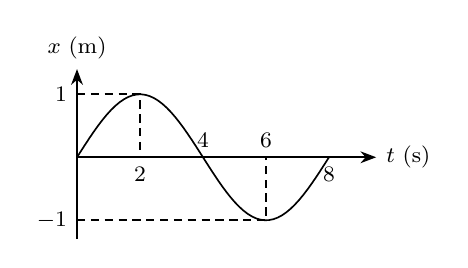
\begin{tikzpicture}[xscale=0.4,yscale=0.8]
\draw[->] (0,0) -- (9.5,0) node[right,lbl]{$t$ (s)}; \draw[->] (0,-1.3) -- (0,1.4) node[above,lbl]{$x$ (m)};
\draw[domain=0:8,samples=60] plot (\x,{sin(45*\x)});
\draw[densely dashed] (0,1) node[left,lbl]{1} -- (2,1) -- (2,0) node[below,lbl]{2} (0,-1) node[left,lbl]{$-1$} -- (6,-1) -- (6,0) node[above,lbl]{6};
\node[lbl,above] at (4,0) {4}; \node[lbl,below] at (8,0) {8};
\end{tikzpicture}}\ntag{A}{266}{keph206}{8}{}{Class XI Part 2 \textperiodcentered{} Ch 13}}
{\opt{$-\dfrac{\pi^2}{16}\unit{m\,s^{-2}}$}{$\dfrac{\pi^2}8\unit{m\,s^{-2}}$}{$-\dfrac{\pi^2}8\unit{m\,s^{-2}}$}{$\dfrac{\pi^2}{16}\unit{m\,s^{-2}}$}}
\numoptstrue
\QQ{\qsrc{2022}{36}Two pendulums of length $121\unit{cm}$ and $100\unit{cm}$ start vibrating in phase. At some instant, the two are at their mean position in the same phase. The minimum number of vibrations of the shorter pendulum after which the two are again in phase at the mean position is:\ntag{A}{271}{keph206}{13}{}{Class XI Part 2 \textperiodcentered{} Ch 13}}
{\opt{8}{11}{9}{10}}
\numoptstrue
\QQ{\qsrc{2021}{3}A body is executing simple harmonic motion with frequency `$n$', the frequency of its potential energy is:\ntag{D}{269}{keph206}{11}{ \textperiodcentered{} K and U have period T/2}{Class XI Part 2 \textperiodcentered{} Ch 13}}
{\opt{$n$}{$2n$}{$3n$}{$4n$}}
\numoptstrue
\QQ{\qsrc{2021}{15}A spring is stretched by $5\unit{cm}$ by a force $10\unit{N}$. The time period of the oscillations when a mass of $2\unit{kg}$ is suspended by it is:\ntag{D}{267}{keph206}{9}{ \textperiodcentered{} omega=sqrt(k/m)}{Class XI Part 2 \textperiodcentered{} Ch 13}}
{\opt{0.0628\,s}{6.28\,s}{3.14\,s}{0.628\,s}}
\numoptstrue
\QQ{\qsrc{2020}{145}The phase difference between displacement and acceleration of a particle in a simple harmonic motion is:\ntag{D}{266}{keph206}{8}{ \textperiodcentered{} a=-omega\textasciicircum{}2 x}{Class XI Part 2 \textperiodcentered{} Ch 13}}
{\opt{$\pi$ rad}{$\dfrac{3\pi}2$ rad}{$\dfrac\pi2$ rad}{zero}}
\numoptstrue
\QQ{\qsrc{2019}{10}The displacement of a particle executing simple harmonic motion is given by $y = A_0+A\sin\omega t+B\cos\omega t$. Then the amplitude of its oscillation is given by:\ntag{D}{262}{keph206}{4}{ \textperiodcentered{} A sin wt + B cos wt = D sin(wt+phi)}{Class XI Part 2 \textperiodcentered{} Ch 13}}
{\opt{$A_0+\sqrt{A^2+B^2}$}{$\sqrt{A^2+B^2}$}{$\sqrt{A_0^2+(A+B)^2}$}{$A+B$}}
\numoptstrue
\QQ{\qsrc{2019}{19}Average velocity of a particle executing SHM in one complete vibration is:\ntag{A}{266}{keph206}{8}{}{Class XI Part 2 \textperiodcentered{} Ch 13}}
{\opt{$\dfrac{A\omega}2$}{$A\omega$}{$\dfrac{A\omega^2}2$}{zero}}
\numoptstrue
\QQ{\qsrc{2019}{42}The radius of circle, the period of revolution, initial position and sense of revolution are indicated in the fig.
\fig{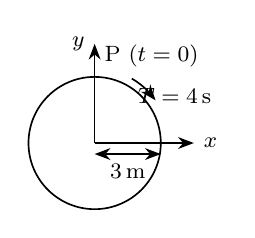
\begin{tikzpicture}[scale=0.7]
\draw (0,0) circle (1.2); \draw[->] (0,0) -- (0,1.8) node[left,lbl]{$y$}; \draw[->] (0,0) -- (1.8,0) node[right,lbl]{$x$};
\node[lbl,above right] at (0,1.2) {P ($t = 0$)}; \draw[->] (60:1.35) arc (60:35:1.35); \node[lbl] at (1.45,0.85) {$T = 4\unit{s}$};
\draw[<->] (0,-0.2) -- (1.2,-0.2) node[midway,below,lbl]{3\,m};
\end{tikzpicture}}
$y$-projection of the radius vector of rotating particle P is:\ntag{D}{265}{keph206}{7}{ \textperiodcentered{} reference circle}{Class XI Part 2 \textperiodcentered{} Ch 13}}
{\opt{$y(t) = -3\cos2\pi t$, where $y$ in m}{$y(t) = 4\sin\left(\dfrac{\pi t}2\right)$, where $y$ in m}{$y(t) = 3\cos\left(\dfrac{3\pi t}2\right)$, where $y$ in m}{$y(t) = 3\cos\left(\dfrac{\pi t}2\right)$, where $y$ in m}}
\numoptstrue
\QQ{\qsrc{2018}{25}A pendulum is hung from the roof of a sufficiently high building and is moving freely to and fro like a simple harmonic oscillator. The acceleration of the bob of the pendulum is $20\unit{m/s^2}$ at a distance of $5\unit{m}$ from the mean position. The time period of oscillation is\ntag{D}{266}{keph206}{8}{ \textperiodcentered{} a=-omega\textasciicircum{}2 x}{Class XI Part 2 \textperiodcentered{} Ch 13}}
{\opt{2\,s}{$\pi$\,s}{$2\pi$\,s}{1\,s}}
\numoptstrue
\QQ{\qsrc{2017}{170}A spring of force constant $k$ is cut into lengths of ratio 1:2:3. They are connected in series and the new force constant is $k'$. Then they are connected in parallel and force constant is $k''$. Then $k':k''$ is:\ntag{A}{267}{keph206}{9}{ \textperiodcentered{} Example 13.6 setting}{Class XI Part 2 \textperiodcentered{} Ch 13}}
{\opt{1:9}{1:11}{1:14}{1:6}}
\numoptstrue
\QQ{\qsrc{2017}{175}A particle executes linear simple harmonic motion with an amplitude of $3\unit{cm}$. When the particle is at $2\unit{cm}$ from the mean position, the magnitude of its velocity is equal to that of its acceleration. Then its time period in seconds is:\ntag{A}{266}{keph206}{8}{}{Class XI Part 2 \textperiodcentered{} Ch 13}}
{\opt{$\dfrac{\sqrt5}{2\pi}$}{$\dfrac{4\pi}{\sqrt5}$}{$\dfrac{2\pi}{\sqrt3}$}{$\dfrac{\sqrt5}\pi$}}
\end{multicols}
\par\needspace{12\baselineskip}\vspace{12pt}
\begin{center}{\pgfornament[width=3.2cm,color=gilt]{87}}\par
{\large\color{navy}\scshape Oscillations \textperiodcentered{} Answer Key}\end{center}
{\small\setlength{\tabcolsep}{1pt}\renewcommand{\arraystretch}{1.5}
\begin{tabularx}{\linewidth}{@{}*{8}{>{\centering\arraybackslash}X}@{}}\toprule
\textbf{1}\,(4) & \textbf{2}\,(2) & \textbf{3}\,(2) & \textbf{4}\,(4) & \textbf{5}\,(3) & \textbf{6}\,(3) & \textbf{7}\,(1) & \textbf{8}\,(2)\\
\textbf{9}\,(2) & \textbf{10}\,(4) & \textbf{11}\,(1) & \textbf{12}\,(2) & \textbf{13}\,(4) & \textbf{14}\,(4) & \textbf{15}\,(2) & \textbf{16}\,(2)\\
\textbf{17}\,(2) &  &  &  &  &  &  & \\\bottomrule\end{tabularx}}\par\smallskip
{\footnotesize Answers of 2021, 2022, 2023, 2025 and 2026 are from the official NTA final keys (checked by the editor); answers of 2016--2020 and 2024 were solved by the editor.
}\par
\par\needspace{18\baselineskip}\vspace{14pt}
\begin{center}{\pgfornament[width=3.2cm,color=gilt]{87}}\par
{\large\color{navy}\scshape Chapter Summary \textperiodcentered{} Oscillations}\end{center}
{\small\setlength{\tabcolsep}{3.5pt}
\begin{tabular*}{\linewidth}{@{\extracolsep{\fill}}l*{11}{c}c@{}}\toprule
Year & 2016 & 2017 & 2018 & 2019 & 2020 & 2021 & 2022 & 2023 & 2024 & 2025 & 2026 & Total\\\midrule
Questions & 0 & 2 & 1 & 3 & 1 & 2 & 1 & 1 & 2 & 2 & 2 & \textbf{17}\\\bottomrule\end{tabular*}}\par\medskip
{\small\textbf{\color{crimson}Topic-wise} (in textbook order)\par\smallskip
\begin{tabularx}{\linewidth}{@{}>{\raggedright\arraybackslash}Xrrrl@{}}\toprule
Topic & Qs & Direct & Years & 2016 $\rightarrow$ 2026\\\midrule
Simple harmonic motion & \textbf{17} & 9 & 10 & {\scriptsize {\color{gray!45}16} \textbf{17} \textbf{18} \textbf{19} \textbf{20} \textbf{21} \textbf{22} \textbf{23} \textbf{24} \textbf{25} \textbf{26}}\\
\bottomrule\end{tabularx}}\par\medskip
\begin{minipage}[t]{0.34\linewidth}{\small\textbf{\color{crimson}Direct vs Applied}\par\smallskip
\begin{tabular}{@{}lrr@{}}\toprule
Direct from NCERT & \textbf{9} & 53\%\\
\quad text, table, figure & 8 &\\
\quad solved Example & 0 &\\
\quad Exercise & 1 &\\
Applied & \textbf{8} & 47\%\\\midrule
Easy / Mod. / Hard & \multicolumn{2}{r}{8 / 9 / 0}\\\bottomrule
\end{tabular}}\end{minipage}\hfill
\begin{minipage}[t]{0.63\linewidth}{\small\textbf{\color{crimson}What to focus on}\par\smallskip
\begin{itemize}[leftmargin=1.1em,itemsep=1pt,topsep=0pt]
\item 17 questions in 11 papers, about 1.5 per paper; rank 13 of 28 chapters by number of questions.
\item Most asked topic: \textbf{Simple harmonic motion} (17 questions, in 10 of the 11 years).
\item Asked in 8 or more of the 11 years: Simple harmonic motion.
\item 1 questions are NCERT solved Examples or Exercises: Exercise 13.17 (Q 1). Work these by hand.
\item NCERT pages that gave three or more questions: page 266 (7 questions), page 267 (3 questions). Read these pages line by line.
\item Difficulty: 8 easy, 9 moderate, 0 hard.
\item 8 applied questions: practise these after the NCERT Examples and Exercises of the chapter.
\end{itemize}}\end{minipage}\par
\chapterpaper{Class XI \textperiodcentered{} Chapter 14}{Waves}{10 questions \textperiodcentered{} 2 topics \textperiodcentered{} NEET 2016--2026}{ckeph207}{XI.14 Waves}
\begin{multicols}{2}
\topichead{Wave motion and speed of waves}{2}
\numoptstrue
\QQ{\qsrc{2022}{5}If the initial tension on a stretched string is doubled, then the ratio of the initial and final speeds of a transverse wave along the string is:\ntag{D}{285}{keph207}{8}{ \textperiodcentered{} v=sqrt(T/mu)}{Class XI Part 2 \textperiodcentered{} Ch 14}}
{\opt{1:2}{1:1}{$\sqrt2:1$}{$1:\sqrt2$}}
\numoptstrue
\QQ{\qsrc{2016}{10}A uniform rope of length $L$ and mass $m_1$ hangs vertically from a rigid support. A block of mass $m_2$ is attached to the free end of the rope. A transverse pulse of wavelength $\lambda_1$ is produced at the lower end of the rope. The wavelength of the pulse when it reaches the top of the rope is $\lambda_2$. The ratio $\lambda_2/\lambda_1$ is:\ntag{A}{285}{keph207}{8}{ \textperiodcentered{} v=sqrt(T/mu)}{Class XI Part 2 \textperiodcentered{} Ch 14}}
{\opt{$\sqrt{\dfrac{m_1}{m_2}}$}{$\sqrt{\dfrac{m_1+m_2}{m_2}}$}{$\sqrt{\dfrac{m_2}{m_1}}$}{$\sqrt{\dfrac{m_1+m_2}{m_1}}$}}
\topichead{Beats, organ pipes and strings}{8}
\numoptstrue
\QQ{\qsrc{2026}{4}For sound waves, if the number of nodes for the $5^{\text{th}}$ harmonic of an open-ended pipe is $n$ and that for the $9^{\text{th}}$ harmonic of the same pipe with one of its ends closed is $m$, the ratio $\dfrac nm$ is\ntag{A}{292}{keph207}{15}{}{Class XI Part 2 \textperiodcentered{} Ch 14}}
{\opt{$\dfrac59$}{$\dfrac95$}{1}{$\dfrac35$}}
\numoptstrue
\QQ{\qsrc{2025}{45}A pipe open at both ends has a fundamental frequency $f$ in air. The pipe is now dipped vertically in a water drum to half of its length. The fundamental frequency of the air column is now equal to:\ntag{A}{292}{keph207}{15}{}{Class XI Part 2 \textperiodcentered{} Ch 14}}
{\opt{$\dfrac f2$}{$f$}{$\dfrac{3f}2$}{$2f$}}
\numoptstrue
\QQ{\qsrc{2023}{14}The ratio of frequencies of fundamental harmonic produced by an open pipe to that of closed pipe having the same length is:\ntag{D}{292}{keph207}{15}{ \textperiodcentered{} open v/2L, closed v/4L}{Class XI Part 2 \textperiodcentered{} Ch 14}}
{\opt{3:1}{1:2}{2:1}{1:3}}
\numoptstrue
\QQ{\qsrc{2020}{147}In a guitar, two strings A and B made of same material are slightly out of tune and produce beats of frequency 6\,Hz. When tension in B is slightly decreased, the beat frequency increases to 7\,Hz. If the frequency of A is 530\,Hz, the original frequency of B will be:\ntag{D}{294}{keph207}{17}{ \textperiodcentered{} Example 14.6}{Class XI Part 2 \textperiodcentered{} Ch 14}}
{\opt{523\,Hz}{524\,Hz}{536\,Hz}{537\,Hz}}
\numoptstrue
\QQ{\qsrc{2018}{2}The fundamental frequency in an open organ pipe is equal to the third harmonic of a closed organ pipe. If the length of the closed organ pipe is $20\unit{cm}$, the length of the open organ pipe is\ntag{A}{292}{keph207}{15}{}{Class XI Part 2 \textperiodcentered{} Ch 14}}
{\opt{12.5\,cm}{8\,cm}{13.2\,cm}{16\,cm}}
\numoptstrue
\QQ{\qsrc{2018}{24}A tuning fork is used to produce resonance in a glass tube. The length of the air column in this tube can be adjusted by a variable piston. At room temperature of $27^\circ$C two successive resonances are produced at $20\unit{cm}$ and $73\unit{cm}$ of column length. If the frequency of the tuning fork is 320\,Hz, the velocity of sound in air at $27^\circ$C is\ntag{D}{299}{keph207}{22}{ \textperiodcentered{} Exercise 14.15}{Class XI Part 2 \textperiodcentered{} Ch 14}}
{\opt{350\,m/s}{339\,m/s}{330\,m/s}{300\,m/s}}
\numoptstrue
\QQ{\qsrc{2017}{157}The two nearest harmonics of a tube closed at one end and open at other end are 220\,Hz and 260\,Hz. What is the fundamental frequency of the system?\ntag{A}{293}{keph207}{16}{ \textperiodcentered{} odd harmonics}{Class XI Part 2 \textperiodcentered{} Ch 14}}
{\opt{20\,Hz}{30\,Hz}{40\,Hz}{10\,Hz}}
\numoptstrue
\QQ{\qsrc{2016}{12}An air column, closed at one end and open at the other, resonates with a tuning fork when the smallest length of the column is $50\unit{cm}$. The next larger length of the column resonating with the same tuning fork is:\ntag{A}{293}{keph207}{16}{ \textperiodcentered{} odd harmonics}{Class XI Part 2 \textperiodcentered{} Ch 14}}
{\opt{66.7\,cm}{100\,cm}{150\,cm}{200\,cm}}
\end{multicols}
\par\needspace{12\baselineskip}\vspace{12pt}
\begin{center}{\pgfornament[width=3.2cm,color=gilt]{87}}\par
{\large\color{navy}\scshape Waves \textperiodcentered{} Answer Key}\end{center}
{\small\setlength{\tabcolsep}{1pt}\renewcommand{\arraystretch}{1.5}
\begin{tabularx}{\linewidth}{@{}*{8}{>{\centering\arraybackslash}X}@{}}\toprule
\textbf{1}\,(4) & \textbf{2}\,(2) & \textbf{3}\,(3) & \textbf{4}\,(2) & \textbf{5}\,(3) & \textbf{6}\,(2) & \textbf{7}\,(3) & \textbf{8}\,(2)\\
\textbf{9}\,(1) & \textbf{10}\,(3) &  &  &  &  &  & \\\bottomrule\end{tabularx}}\par\smallskip
{\footnotesize Answers of 2021, 2022, 2023, 2025 and 2026 are from the official NTA final keys (checked by the editor); answers of 2016--2020 and 2024 were solved by the editor.
}\par
\par\needspace{18\baselineskip}\vspace{14pt}
\begin{center}{\pgfornament[width=3.2cm,color=gilt]{87}}\par
{\large\color{navy}\scshape Chapter Summary \textperiodcentered{} Waves}\end{center}
{\small\setlength{\tabcolsep}{3.5pt}
\begin{tabular*}{\linewidth}{@{\extracolsep{\fill}}l*{11}{c}c@{}}\toprule
Year & 2016 & 2017 & 2018 & 2019 & 2020 & 2021 & 2022 & 2023 & 2024 & 2025 & 2026 & Total\\\midrule
Questions & 2 & 1 & 2 & 0 & 1 & 0 & 1 & 1 & 0 & 1 & 1 & \textbf{10}\\\bottomrule\end{tabular*}}\par\medskip
{\small\textbf{\color{crimson}Topic-wise} (in textbook order)\par\smallskip
\begin{tabularx}{\linewidth}{@{}>{\raggedright\arraybackslash}Xrrrl@{}}\toprule
Topic & Qs & Direct & Years & 2016 $\rightarrow$ 2026\\\midrule
Wave motion and speed of waves & \textbf{2} & 1 & 2 & {\scriptsize \textbf{16} {\color{gray!45}17} {\color{gray!45}18} {\color{gray!45}19} {\color{gray!45}20} {\color{gray!45}21} \textbf{22} {\color{gray!45}23} {\color{gray!45}24} {\color{gray!45}25} {\color{gray!45}26}}\\
Beats, organ pipes and strings & \textbf{8} & 3 & 7 & {\scriptsize \textbf{16} \textbf{17} \textbf{18} {\color{gray!45}19} \textbf{20} {\color{gray!45}21} {\color{gray!45}22} \textbf{23} {\color{gray!45}24} \textbf{25} \textbf{26}}\\
\bottomrule\end{tabularx}}\par\medskip
\begin{minipage}[t]{0.34\linewidth}{\small\textbf{\color{crimson}Direct vs Applied}\par\smallskip
\begin{tabular}{@{}lrr@{}}\toprule
Direct from NCERT & \textbf{4} & 40\%\\
\quad text, table, figure & 2 &\\
\quad solved Example & 1 &\\
\quad Exercise & 1 &\\
Applied & \textbf{6} & 60\%\\\midrule
Easy / Mod. / Hard & \multicolumn{2}{r}{4 / 6 / 0}\\\bottomrule
\end{tabular}}\end{minipage}\hfill
\begin{minipage}[t]{0.63\linewidth}{\small\textbf{\color{crimson}What to focus on}\par\smallskip
\begin{itemize}[leftmargin=1.1em,itemsep=1pt,topsep=0pt]
\item 10 questions in 11 papers, about 0.9 per paper; rank 25 of 28 chapters by number of questions.
\item Most asked topic: \textbf{Beats, organ pipes and strings} (8 questions, in 7 of the 11 years).
\item 2 questions are NCERT solved Examples or Exercises: Example 14.6 (Q 6), Exercise 14.15 (Q 8). Work these by hand.
\item NCERT pages that gave three or more questions: page 292 (4 questions). Read these pages line by line.
\item Difficulty: 4 easy, 6 moderate, 0 hard.
\item 6 applied questions: practise these after the NCERT Examples and Exercises of the chapter.
\end{itemize}}\end{minipage}\par
\chapterpaper{Class XII \textperiodcentered{} Chapter 1}{Electric Charges and Fields}{13 questions \textperiodcentered{} 4 topics \textperiodcentered{} NEET 2016--2026}{cleph101}{XII.1 Electric Charges and Fields}
\begin{multicols}{2}
\topichead{Electric charge and Coulomb's law}{4}
\numoptstrue
\QQ{\qsrc{2025}{28}Two identical charged conducting spheres A and B have their centres separated by a certain distance. Charge on each sphere is $q$ and the force of repulsion between them is $F$. A third identical uncharged conducting sphere is brought in contact with sphere A first and then with B and finally removed from both. New force of repulsion between spheres A and B (radii of A and B are negligible compared to the distance of separation so that for calculating force between them they can be considered as point charges) is best given as:\ntag{A}{10}{leph101}{10}{}{Class XII Part 1 \textperiodcentered{} Ch 1}}
{\opt{$\dfrac{3F}5$}{$\dfrac{2F}3$}{$\dfrac F2$}{$\dfrac{3F}8$}}
\numoptstrue
\QQ{\qsrc{2019}{37}Two point charges A and B, having charges $+Q$ and $-Q$ respectively, are placed at certain distance apart and force acting between them is $F$. If 25\% charge of A is transferred to B, then force between the charges becomes:\ntag{A}{8}{leph101}{8}{}{Class XII Part 1 \textperiodcentered{} Ch 1}}
{\opt{$F$}{$\dfrac{9F}{16}$}{$\dfrac{16F}9$}{$\dfrac{4F}3$}}
\numoptstrue
\QQ{\qsrc{2017}{172}Suppose the charge of a proton and an electron differ slightly. One of them is $-e$, the other is $(e+\Delta e)$. If the net of electrostatic force and gravitational force between two hydrogen atoms placed at a distance $d$ (much greater than atomic size) apart is zero, then $\Delta e$ is of the order of [Given mass of hydrogen $m_h = 1.67\times10^{-27}\unit{kg}$]\ntag{A}{9}{leph101}{9}{}{Class XII Part 1 \textperiodcentered{} Ch 1}}
{\opt{$10^{-23}\unit{C}$}{$10^{-37}\unit{C}$}{$10^{-47}\unit{C}$}{$10^{-20}\unit{C}$}}
\numoptstrue
\QQ{\qsrc{2016}{9}Two identical charged spheres suspended from a common point by two massless strings of lengths $l$, are initially at a distance $d$ ($d\ll l$) apart because of their mutual repulsion. The charges begin to leak from both the spheres at a constant rate. As a result, the spheres approach each other with a velocity $v$. Then $v$ varies as a function of the distance $x$ between the spheres, as:\ntag{A}{9}{leph101}{9}{}{Class XII Part 1 \textperiodcentered{} Ch 1}}
{\opt{$v\propto x^{1/2}$}{$v\propto x$}{$v\propto x^{-1/2}$}{$v\propto x^{-1}$}}
\topichead{Coulomb force and electric field}{1}
\numoptstrue
\QQ{\qsrc{2018}{22}An electron falls from rest through a vertical distance $h$ in a uniform and vertically upward directed electric field E. The direction of electric field is now reversed, keeping its magnitude the same. A proton is allowed to fall from rest in it through the same vertical distance $h$. The time of fall of the electron, in comparison to the time of fall of the proton is\ntag{D}{17}{leph101}{17}{ \textperiodcentered{} Example 1.7}{Class XII Part 1 \textperiodcentered{} Ch 1}}
{\opt{10 times greater}{5 times greater}{smaller}{equal}}
\topichead{Electric dipole}{4}
\numoptstrue
\QQ{\qsrc{2023}{9}An electric dipole is placed at an angle of $30^\circ$ with an electric field of intensity $2\times10^5\unit{N\,C^{-1}}$. It experiences a torque equal to $4\unit{N\,m}$. Calculate the magnitude of charge on the dipole, if the dipole length is $2\unit{cm}$.\ntag{D}{27}{leph101}{27}{ \textperiodcentered{} tau=pE sin theta}{Class XII Part 1 \textperiodcentered{} Ch 1}}
{\opt{2\,mC}{8\,mC}{6\,mC}{4\,mC}}
\numoptstrue
\QQ{\qsrc{2022}{49}Two point charges $-q$ and $+q$ are placed at a distance of $L$, as shown in the figure.
\fig{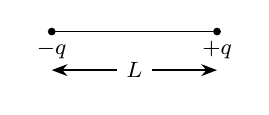
\begin{tikzpicture}[scale=0.7]
\fill (0,0) circle (2pt) node[below,lbl]{$-q$}; \fill (3,0) circle (2pt) node[below,lbl]{$+q$}; \draw (0,0) -- (3,0); \draw[<->] (0,-0.7) -- (3,-0.7) node[midway,fill=white,lbl]{$L$};
\end{tikzpicture}}
The magnitude of electric field intensity at a distance $R$ ($R\gg L$) varies as:\ntag{D}{25}{leph101}{25}{ \textperiodcentered{} dipole field falls as 1/r\textasciicircum{}3}{Class XII Part 1 \textperiodcentered{} Ch 1}}
{\opt{$\dfrac1{R^6}$}{$\dfrac1{R^2}$}{$\dfrac1{R^3}$}{$\dfrac1{R^4}$}}
\numoptstrue
\QQ{\qsrc{2021}{6}A dipole is placed in an electric field as shown. In which direction will it move?
\fig{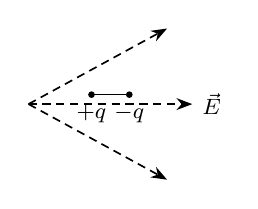
\begin{tikzpicture}[scale=0.8]
\draw[densely dashed,->] (0,0) -- (2.6,0) node[right,lbl]{$\vec E$}; \draw[densely dashed,->] (0,0) -- (2.2,1.2); \draw[densely dashed,->] (0,0) -- (2.2,-1.2);
\fill (1.0,0.15) circle (1.5pt) node[below,lbl]{$+q$}; \fill (1.6,0.15) circle (1.5pt) node[below,lbl]{$-q$}; \draw (1.0,0.15) -- (1.6,0.15);
\end{tikzpicture}}\ntag{A}{27}{leph101}{27}{}{Class XII Part 1 \textperiodcentered{} Ch 1}}
{\opt{towards the left as its potential energy will increase.}{towards the right as its potential energy will decrease.}{towards the left as its potential energy will decrease.}{towards the right as its potential energy will increase.}}
\numoptstrue
\QQ{\qsrc{2021}{25}Polar molecules are the molecules:\ntag{D}{25}{leph101}{25}{ \textperiodcentered{} polar molecules}{Class XII Part 1 \textperiodcentered{} Ch 1}}
{\opt{having zero dipole moment.}{acquire a dipole moment only in the presence of electric field due to displacement of charges.}{acquire a dipole moment only when magnetic field is absent.}{having a permanent electric dipole moment.}}
\topichead{Gauss's law and electric flux}{4}
\numoptstrue
\QQ{\qsrc{2023}{17}If $\displaystyle\oint_S\vec E\cdot d\vec S = 0$ over a surface, then:\ntag{D}{31}{leph101}{31}{ \textperiodcentered{} zero net flux}{Class XII Part 1 \textperiodcentered{} Ch 1}}
{\opt{the electric field inside the surface is necessarily uniform.}{the number of flux lines entering the surface must be equal to the number of flux lines leaving it.}{the magnitude of electric field on the surface is constant.}{all the charges must necessarily be inside the surface.}}
\numoptstrue
\QQ{\qsrc{2020}{151}A spherical conductor of radius $10\unit{cm}$ has a charge of $3.2\times10^{-7}\unit{C}$ distributed uniformly. What is the magnitude of electric field at a point $15\unit{cm}$ from the centre of the sphere? $\left(\dfrac1{4\pi\varepsilon_0} = 9\times10^9\unit{N\,m^2/C^2}\right)$\ntag{D}{35}{leph101}{35}{ \textperiodcentered{} shell: field outside q/4 pi eps0 r\textasciicircum{}2}{Class XII Part 1 \textperiodcentered{} Ch 1}}
{\opt{$1.28\times10^4\unit{N/C}$}{$1.28\times10^5\unit{N/C}$}{$1.28\times10^6\unit{N/C}$}{$1.28\times10^7\unit{N/C}$}}
\numoptstrue
\QQ{\qsrc{2019}{25}A hollow metal sphere of radius $R$ is uniformly charged. The electric field due to the sphere at a distance $r$ from the centre:\ntag{D}{36}{leph101}{36}{ \textperiodcentered{} shell: zero inside, kq/r\textasciicircum{}2 outside}{Class XII Part 1 \textperiodcentered{} Ch 1}}
{\opt{increases as $r$ increases for $r<R$ and for $r>R$}{zero as $r$ increases for $r<R$, decreases as $r$ increases for $r>R$}{zero as $r$ increases for $r<R$, increases as $r$ increases for $r>R$}{decreases as $r$ increases for $r<R$ and for $r>R$}}
\numoptstrue
\QQ{\qsrc{2019}{36}Two parallel infinite line charges with linear charge densities $+\lambda$\,C/m and $-\lambda$\,C/m are placed at a distance of $2R$ in free space. What is the electric field mid-way between the two line charges?\ntag{A}{34}{leph101}{34}{}{Class XII Part 1 \textperiodcentered{} Ch 1}}
{\opt{zero}{$\dfrac{2\lambda}{\pi\varepsilon_0R}$\,N/C}{$\dfrac\lambda{\pi\varepsilon_0R}$\,N/C}{$\dfrac\lambda{2\pi\varepsilon_0R}$\,N/C}}
\end{multicols}
\par\needspace{12\baselineskip}\vspace{12pt}
\begin{center}{\pgfornament[width=3.2cm,color=gilt]{87}}\par
{\large\color{navy}\scshape Electric Charges and Fields \textperiodcentered{} Answer Key}\end{center}
{\small\setlength{\tabcolsep}{1pt}\renewcommand{\arraystretch}{1.5}
\begin{tabularx}{\linewidth}{@{}*{8}{>{\centering\arraybackslash}X}@{}}\toprule
\textbf{1}\,(4) & \textbf{2}\,(2) & \textbf{3}\,(2) & \textbf{4}\,(3) & \textbf{5}\,(3) & \textbf{6}\,(1) & \textbf{7}\,(3) & \textbf{8}\,(3)\\
\textbf{9}\,(4) & \textbf{10}\,(2) & \textbf{11}\,(2) & \textbf{12}\,(2) & \textbf{13}\,(3) &  &  & \\\bottomrule\end{tabularx}}\par\smallskip
{\footnotesize Answers of 2021, 2022, 2023, 2025 and 2026 are from the official NTA final keys (checked by the editor); answers of 2016--2020 and 2024 were solved by the editor.
}\par
\par\needspace{18\baselineskip}\vspace{14pt}
\begin{center}{\pgfornament[width=3.2cm,color=gilt]{87}}\par
{\large\color{navy}\scshape Chapter Summary \textperiodcentered{} Electric Charges and Fields}\end{center}
{\small\setlength{\tabcolsep}{3.5pt}
\begin{tabular*}{\linewidth}{@{\extracolsep{\fill}}l*{11}{c}c@{}}\toprule
Year & 2016 & 2017 & 2018 & 2019 & 2020 & 2021 & 2022 & 2023 & 2024 & 2025 & 2026 & Total\\\midrule
Questions & 1 & 1 & 1 & 3 & 1 & 2 & 1 & 2 & 0 & 1 & 0 & \textbf{13}\\\bottomrule\end{tabular*}}\par\medskip
{\small\textbf{\color{crimson}Topic-wise} (in textbook order)\par\smallskip
\begin{tabularx}{\linewidth}{@{}>{\raggedright\arraybackslash}Xrrrl@{}}\toprule
Topic & Qs & Direct & Years & 2016 $\rightarrow$ 2026\\\midrule
Electric charge and Coulomb's law & \textbf{4} & 0 & 4 & {\scriptsize \textbf{16} \textbf{17} {\color{gray!45}18} \textbf{19} {\color{gray!45}20} {\color{gray!45}21} {\color{gray!45}22} {\color{gray!45}23} {\color{gray!45}24} \textbf{25} {\color{gray!45}26}}\\
Coulomb force and electric field & \textbf{1} & 1 & 1 & {\scriptsize {\color{gray!45}16} {\color{gray!45}17} \textbf{18} {\color{gray!45}19} {\color{gray!45}20} {\color{gray!45}21} {\color{gray!45}22} {\color{gray!45}23} {\color{gray!45}24} {\color{gray!45}25} {\color{gray!45}26}}\\
Electric dipole & \textbf{4} & 3 & 3 & {\scriptsize {\color{gray!45}16} {\color{gray!45}17} {\color{gray!45}18} {\color{gray!45}19} {\color{gray!45}20} \textbf{21} \textbf{22} \textbf{23} {\color{gray!45}24} {\color{gray!45}25} {\color{gray!45}26}}\\
Gauss's law and electric flux & \textbf{4} & 3 & 3 & {\scriptsize {\color{gray!45}16} {\color{gray!45}17} {\color{gray!45}18} \textbf{19} \textbf{20} {\color{gray!45}21} {\color{gray!45}22} \textbf{23} {\color{gray!45}24} {\color{gray!45}25} {\color{gray!45}26}}\\
\bottomrule\end{tabularx}}\par\medskip
\begin{minipage}[t]{0.34\linewidth}{\small\textbf{\color{crimson}Direct vs Applied}\par\smallskip
\begin{tabular}{@{}lrr@{}}\toprule
Direct from NCERT & \textbf{7} & 54\%\\
\quad text, table, figure & 6 &\\
\quad solved Example & 1 &\\
\quad Exercise & 0 &\\
Applied & \textbf{6} & 46\%\\\midrule
Easy / Mod. / Hard & \multicolumn{2}{r}{7 / 4 / 2}\\\bottomrule
\end{tabular}}\end{minipage}\hfill
\begin{minipage}[t]{0.63\linewidth}{\small\textbf{\color{crimson}What to focus on}\par\smallskip
\begin{itemize}[leftmargin=1.1em,itemsep=1pt,topsep=0pt]
\item 13 questions in 11 papers, about 1.2 per paper; rank 22 of 28 chapters by number of questions.
\item Most asked topic: \textbf{Electric charge and Coulomb's law} (4 questions, in 4 of the 11 years).
\item 1 questions are NCERT solved Examples or Exercises: Example 1.7 (Q 5). Work these by hand.
\item Difficulty: 7 easy, 4 moderate, 2 hard (hard: Q 3, 4).
\item 6 applied questions: practise these after the NCERT Examples and Exercises of the chapter.
\end{itemize}}\end{minipage}\par
\chapterpaper{Class XII \textperiodcentered{} Chapter 2}{Electrostatic Potential and Capacitance}{26 questions \textperiodcentered{} 6 topics \textperiodcentered{} NEET 2016--2026}{cleph102}{XII.2 Electrostatic Potential and Capacitance}
\begin{multicols}{2}
\topichead{Electric potential and potential energy}{7}
\numoptstrue
\QQ{\qsrc{2026}{21}A unit positive point charge is taken slowly through an infinitesimally thin tube that is inside a charged dielectric sphere of radius $R$, having uniform positive charge density $\rho$, as shown in the figure. The initial and final positions of the charge are marked by A and B at distance $2R$ and $3R$ respectively, from the centre of the sphere. In this process, the magnitude of the total work done on the point charge is $\dfrac{\rho R^2}{n\varepsilon_0}$. The value of $n$ is: ($\varepsilon_0$ is the permittivity of vacuum)
\fig{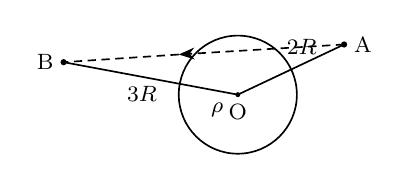
\begin{tikzpicture}[scale=0.75]
\draw (0,0) circle (1);
\fill (0,0) circle (1.2pt) node[below,lbl]{O}; \node[lbl] at (-0.35,-0.25) {$\rho$};
\coordinate (A) at (1.8,0.85); \coordinate (B) at (-2.95,0.55);
\fill (A) circle (1.5pt) node[right,lbl]{A}; \fill (B) circle (1.5pt) node[left,lbl]{B};
\draw[densely dashed,->] (A) -- (-1.0,0.68); \draw[densely dashed] (-1.0,0.68) -- (B);
\draw (0,0) -- (A) node[pos=0.6,above,lbl]{$2R$}; \draw (0,0) -- (B) node[pos=0.55,below,lbl]{$3R$};
\end{tikzpicture}}\ntag{A}{52}{leph102}{8}{}{Class XII Part 1 \textperiodcentered{} Ch 2}}
{\opt{2}{6}{9}{18}}
\numoptstrue
\QQ{\qsrc{2026}{34}Consider a fixed uniformly charged insulating sphere with radius $R$ and total charge $+Q$. A point charge $-q$ ($q\ll Q$) with mass $m$ is released from rest at a distance of $3R$ from the centre of the charged sphere. When the point charge reaches the surface of the sphere, its speed is: ($\varepsilon_0$ is the permittivity of vacuum, neglect gravitational forces).\ntag{A}{55}{leph102}{11}{}{Class XII Part 1 \textperiodcentered{} Ch 2}}
{\opt{$\sqrt{\dfrac{3Qq}{4\pi\varepsilon_0mR}}$}{$\sqrt{\dfrac{2Qq}{3\pi\varepsilon_0mR}}$}{$\sqrt{\dfrac{Qq}{3\pi\varepsilon_0mR}}$}{$\sqrt{\dfrac{Qq}{4\pi\varepsilon_0mR}}$}}
\numoptstrue
\QQ{\qsrc{2024}{14}A thin spherical shell is charged by some source. The potential difference between the two points C and P (in V) shown in the figure is: (Take $\dfrac1{4\pi\varepsilon_0} = 9\times10^9$ SI units)
\fig{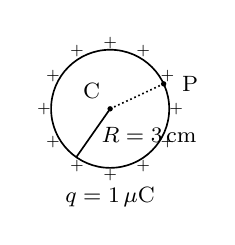
\begin{tikzpicture}[scale=0.75]
\draw (0,0) circle (1); \foreach \a in {0,30,...,330} \node[font=\tiny] at (\a:1.12) {$+$};
\fill (0,0) circle (1.3pt) node[above left,lbl]{C}; \fill (25:1) circle (1.3pt) node[right=3pt,lbl]{P};
\draw[densely dotted] (0,0) -- (25:1); \draw (0,0) -- (-125:1) node[pos=0.55,right,lbl]{$R = 3\unit{cm}$};
\node[lbl] at (0,-1.5) {$q = 1\unit{\mu C}$};
\end{tikzpicture}}\ntag{D}{52}{leph102}{8}{ \textperiodcentered{} V inside a shell is constant}{Class XII Part 1 \textperiodcentered{} Ch 2}}
{\opt{zero}{$3\times10^5$}{$1\times10^5$}{$0.5\times10^5$}}
\numoptstrue
\QQ{\qsrc{2023}{49}An electric dipole is placed as shown in the figure. The electric potential (in $10^2\unit{V}$) at point P due to the dipole is ($\varepsilon_0$ = permittivity of free space and $\dfrac1{4\pi\varepsilon_0} = K$):
\fig{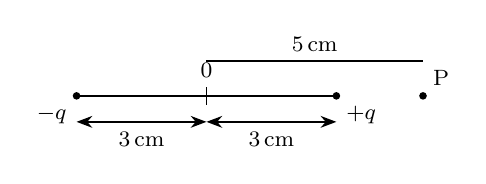
\begin{tikzpicture}[scale=0.55]
\fill (-3,0) circle (2.5pt) node[below left,lbl]{$-q$}; \fill (3,0) circle (2.5pt) node[below right,lbl]{$+q$}; \draw (-3,0) -- (3,0);
\draw (0,-0.2) -- (0,0.2) node[above,lbl]{0}; \fill (5,0) circle (2.5pt) node[above right,lbl]{P};
\draw[<->] (-3,-0.6) -- (0,-0.6) node[midway,below,lbl]{3\,cm}; \draw[<->] (0,-0.6) -- (3,-0.6) node[midway,below,lbl]{3\,cm};
\draw (0,0.8) -- (5,0.8) node[midway,above,lbl]{5\,cm};
\end{tikzpicture}}\ntag{A}{51}{leph102}{7}{}{Class XII Part 1 \textperiodcentered{} Ch 2}}
{\opt{$\left(\dfrac83\right)qK$}{$\left(\dfrac38\right)qK$}{$\left(\dfrac58\right)qK$}{$\left(\dfrac85\right)qK$}}
\numoptstrue
\QQ{\qsrc{2022}{2}Two hollow conducting spheres of radii $R_1$ and $R_2$ ($R_1\gg R_2$) have equal charges. The potential would be:\ntag{D}{52}{leph102}{8}{ \textperiodcentered{} V=kQ/R}{Class XII Part 1 \textperiodcentered{} Ch 2}}
{\opt{dependent on the material property of the sphere}{more on bigger sphere}{more on smaller sphere}{equal on both the spheres}}
\numoptstrue
\QQ{\qsrc{2021}{43}Twenty seven drops of same size are charged at $220\unit{V}$ each. They combine to form a bigger drop. Calculate the potential of the bigger drop.\ntag{A}{48}{leph102}{4}{}{Class XII Part 1 \textperiodcentered{} Ch 2}}
{\opt{660\,V}{1320\,V}{1520\,V}{1980\,V}}
\numoptstrue
\QQ{\qsrc{2020}{159}The energy required to break one bond in DNA is $10^{-20}\unit{J}$. This value in eV is nearly:\ntag{D}{59}{leph102}{15}{ \textperiodcentered{} 1 eV = 1.6e-19 J}{Class XII Part 1 \textperiodcentered{} Ch 2}}
{\opt{6}{0.6}{0.06}{0.006}}
\topichead{Equipotential surfaces and potential gradient}{3}
\numoptstrue
\QQ{\qsrc{2022}{27}The angle between the electric lines of force and the equipotential surface is:\ntag{D}{54}{leph102}{10}{ \textperiodcentered{} E perpendicular to equipotential}{Class XII Part 1 \textperiodcentered{} Ch 2}}
{\opt{$180^\circ$}{$0^\circ$}{$45^\circ$}{$90^\circ$}}
\numoptstrue
\QQ{\qsrc{2020}{152}In a certain region of space with volume $0.2\unit{m^3}$, the electric potential is found to be $5\unit{V}$ throughout. The magnitude of electric field in this region is:\ntag{D}{55}{leph102}{11}{ \textperiodcentered{} E=-dV/dl}{Class XII Part 1 \textperiodcentered{} Ch 2}}
{\opt{zero}{0.5\,N/C}{1\,N/C}{5\,N/C}}
\numoptstrue
\QQ{\qsrc{2017}{171}The diagrams below show regions of equipotentials.
\fig{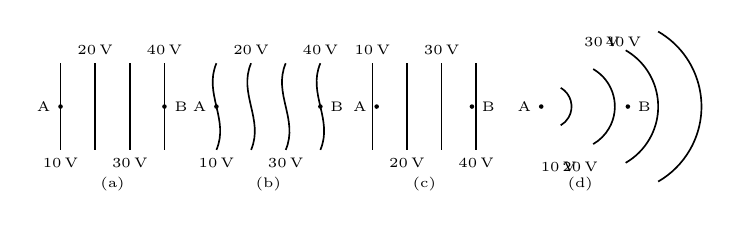
\begin{tikzpicture}[scale=0.55]
\foreach \x/\v in {0/10,0.8/20,1.6/30,2.4/40} {\draw (\x,0) -- (\x,2); \node[font=\tiny] at (\x,{mod(\x*10,16)<1?-0.3:2.3}) {\v\,V};}
\fill (0,1) circle (1.5pt) node[left,font=\tiny]{A}; \fill (2.4,1) circle (1.5pt) node[right,font=\tiny]{B}; \node[font=\tiny] at (1.2,-0.8) {(a)};
\begin{scope}[xshift=3.6cm]
\foreach \x/\v in {0/10,0.8/20,1.6/30,2.4/40} {\draw (\x,0) .. controls (\x+0.3,0.7) and (\x-0.3,1.3) .. (\x,2); \node[font=\tiny] at (\x,{mod(\x*10,16)<1?-0.3:2.3}) {\v\,V};}
\fill (0,1) circle (1.5pt) node[left,font=\tiny]{A}; \fill (2.4,1) circle (1.5pt) node[right,font=\tiny]{B}; \node[font=\tiny] at (1.2,-0.8) {(b)};
\end{scope}
\begin{scope}[xshift=7.2cm]
\foreach \x/\v in {0/10,0.8/20,1.6/30,2.4/40} {\draw (\x,0) -- (\x,2); \node[font=\tiny] at (\x,{mod(\x*10,16)<1?2.3:-0.3}) {\v\,V};}
\fill (0.1,1) circle (1.5pt) node[left,font=\tiny]{A}; \fill (2.3,1) circle (1.5pt) node[right,font=\tiny]{B}; \node[font=\tiny] at (1.2,-0.8) {(c)};
\end{scope}
\begin{scope}[xshift=10.8cm]
\foreach \r/\v in {0.5/10,1.0/20,1.5/30,2.0/40} {\draw (\r,1) ++(60:\r) arc (60:-60:\r); \node[font=\tiny] at (\r+0.2,{\r>1.2?2.5:-0.4}) {\v\,V};}
\fill (0.3,1) circle (1.5pt) node[left,font=\tiny]{A}; \fill (2.3,1) circle (1.5pt) node[right,font=\tiny]{B}; \node[font=\tiny] at (1.2,-0.8) {(d)};
\end{scope}
\end{tikzpicture}}
A positive charge is moved from A to B in each diagram.\ntag{A}{48}{leph102}{4}{ \textperiodcentered{} work independent of path}{Class XII Part 1 \textperiodcentered{} Ch 2}}
{\opt{In all the four cases the work done is the same.}{Minimum work is required to move $q$ in figure (a).}{Maximum work is required to move $q$ in figure (b).}{Maximum work is required to move $q$ in figure (c).}}
\topichead{Electric dipole}{3}
\numoptstrue
\QQ{\qsrc{2025}{35}An electric dipole with dipole moment $5\times10^{-6}\unit{C\,m}$ is aligned with the direction of a uniform electric field of magnitude $4\times10^5\unit{N/C}$. The dipole is then rotated through an angle of $60^\circ$ with respect to the electric field. The change in the potential energy of the dipole is:\ntag{D}{61}{leph102}{17}{ \textperiodcentered{} W=pE(cos theta0 - cos theta1)}{Class XII Part 1 \textperiodcentered{} Ch 2}}
{\opt{0.8\,J}{1.0\,J}{1.2\,J}{1.5\,J}}
\numoptstrue
\QQ{\qsrc{2024}{17}Given below are two statements: one is labelled as \textbf{Assertion A} and the other is labelled as \textbf{Reason R}.\par
\textbf{Assertion A}: The potential ($V$) at any axial point, at $2\unit{m}$ distance ($r$) from the centre of the dipole of dipole moment vector $\vec P$ of magnitude $4\times10^{-6}\unit{C\,m}$, is $\pm9\times10^3\unit{V}$. (Take $\dfrac1{4\pi\varepsilon_0} = 9\times10^9$ SI units)\par
\textbf{Reason R}: $V = \pm\dfrac{2P}{4\pi\varepsilon_0r^2}$, where $r$ is the distance of any axial point, situated at $2\unit{m}$ from the centre of the dipole.\par
In the light of the above statements, choose the \textit{correct} answer from the options given below:\ntag{A}{50}{leph102}{6}{}{Class XII Part 1 \textperiodcentered{} Ch 2}}
{\opt{A is false but R is true.}{Both A and R are true and R is the correct explanation of A.}{Both A and R are true and R is NOT the correct explanation of A.}{A is true but R is false.}}
\numoptstrue
\QQ{\qsrc{2020}{170}A short electric dipole has a dipole moment of $16\times10^{-9}\unit{C\,m}$. The electric potential due to the dipole at a point at a distance of $0.6\unit{m}$ from the centre of the dipole, situated on a line making an angle of $60^\circ$ with the dipole axis is: $\left(\dfrac1{4\pi\varepsilon_0} = 9\times10^9\unit{N\,m^2/C^2}\right)$\ntag{D}{50}{leph102}{6}{ \textperiodcentered{} V=p cos theta/(4 pi eps0 r\textasciicircum{}2)}{Class XII Part 1 \textperiodcentered{} Ch 2}}
{\opt{50\,V}{200\,V}{400\,V}{zero}}
\topichead{Gauss's law and electric flux}{2}
\numoptstrue
\QQ{\qsrc{2026}{33}A point charge $Q$ is placed inside a cavity within a solid isolated conducting sphere. Consider points A, B and C as shown in the figure, where the magnitudes of the electric fields are $E_A$, $E_B$, $E_C$, respectively. The points B and C are at the same distance from the center of the solid sphere. The correct option is:
\fig{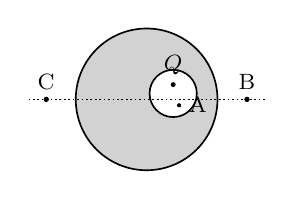
\begin{tikzpicture}[scale=0.75]
\fill[gray!35] (0,0) circle (1.2); \draw (0,0) circle (1.2);
\fill[white] (0.45,0.1) circle (0.4); \draw (0.45,0.1) circle (0.4);
\fill (0.45,0.25) circle (1.2pt) node[above,lbl]{$Q$}; \fill (0.55,-0.1) circle (1pt) node[right,lbl]{A};
\draw[densely dotted] (-2.0,0) -- (2.0,0);
\fill (-1.7,0) circle (1.3pt) node[above,lbl]{C}; \fill (1.7,0) circle (1.3pt) node[above,lbl]{B};
\end{tikzpicture}}\ntag{A}{63}{leph102}{19}{}{Class XII Part 1 \textperiodcentered{} Ch 2}}
{\opt{$E_A = 0$, $E_B = E_C$}{$E_A\ne0$, $E_B = E_C$}{$E_A = 0$, $E_B>E_C$}{$E_A\ne0$, $E_B<E_C$}}
\numoptstrue
\QQ{\qsrc{2021}{28}Two charged spherical conductors of radius $R_1$ and $R_2$ are connected by a wire. Then the ratio of surface charge densities of the spheres ($\sigma_1/\sigma_2$) is:\ntag{A}{63}{leph102}{19}{}{Class XII Part 1 \textperiodcentered{} Ch 2}}
{\opt{$\dfrac{R_1}{R_2}$}{$\dfrac{R_2}{R_1}$}{$\sqrt{\dfrac{R_1}{R_2}}$}{$\dfrac{R_1^2}{R_2^2}$}}
\topichead{Capacitors (energy, dielectrics)}{7}
\numoptstrue
\QQ{\qsrc{2025}{20}The plates of a parallel plate capacitor are separated by $d$. Two slabs of different dielectric constant $K_1$ and $K_2$ with thickness $\dfrac38d$ and $\dfrac d2$, respectively are inserted in the capacitor. Due to this, the capacitance becomes two times larger than when there is nothing between the plates. If $K_1 = 1.25K_2$, the value of $K_1$ is:\ntag{A}{71}{leph102}{27}{}{Class XII Part 1 \textperiodcentered{} Ch 2}}
{\opt{2.66}{2.33}{1.60}{1.33}}
\numoptstrue
\QQ{\qsrc{2024}{37}If the plates of a parallel plate capacitor connected to a battery are moved close to each other, then
\begin{stmts}[\Alph*.]
\item the charge stored in it, increases.
\item the energy stored in it, decreases.
\item its capacitance increases.
\item the ratio of charge to its potential remains the same.
\item the product of charge and voltage increases.
\end{stmts}
Choose the most appropriate answer from the options given below:\ntag{A}{69}{leph102}{25}{}{Class XII Part 1 \textperiodcentered{} Ch 2}}
{\opt{A, B and C only}{A, B and E only}{A, C and E only}{B, D and E only}}
\numoptstrue
\QQ{\qsrc{2022}{50}A capacitor of capacitance $C = 900\unit{pF}$ is charged fully by $100\unit{V}$ battery B as shown in figure (a). Then it is disconnected from the battery and connected to another uncharged capacitor of capacitance $C = 900\unit{pF}$ as shown in figure (b). The electrostatic energy stored by the system (b) is:
\fig{\begin{circuitikz}[scale=0.55,transform shape,font=\Large]
\draw (0,2) to[C,l=$C$] (2,2) -- (2,0) to[battery1,l_={100\,V}] (0,0) -- (0,2); \node at (1,-1.1) {(a)};
\draw (3.5,2) to[C,l=$C$] (5.5,2) -- (5.5,0) to[C,l_=$C$] (3.5,0) -- (3.5,2); \node at (4.5,-1.1) {(b)};
\end{circuitikz}}\ntag{D}{75}{leph102}{31}{ \textperiodcentered{} Example 2.10}{Class XII Part 1 \textperiodcentered{} Ch 2}}
{\opt{$1.5\times10^{-6}\unit{J}$}{$4.5\times10^{-6}\unit{J}$}{$3.25\times10^{-6}\unit{J}$}{$2.25\times10^{-6}\unit{J}$}}
\numoptstrue
\QQ{\qsrc{2021}{16}A parallel plate capacitor has a uniform electric field `$\vec E$' in the space between the plates. If the distance between the plates is `$d$' and the area of each plate is `$A$', the energy stored in the capacitor is: ($\varepsilon_0$ = permittivity of free space)\ntag{D}{75}{leph102}{31}{ \textperiodcentered{} energy density (1/2)eps0 E\textasciicircum{}2}{Class XII Part 1 \textperiodcentered{} Ch 2}}
{\opt{$\dfrac12\varepsilon_0E^2$}{$\varepsilon_0EAd$}{$\dfrac12\varepsilon_0E^2Ad$}{$\dfrac{E^2Ad}{\varepsilon_0}$}}
\numoptstrue
\QQ{\qsrc{2020}{166}The capacitance of a parallel plate capacitor with air as medium is $6\unit{\mu F}$. With the introduction of a dielectric medium, the capacitance becomes $30\unit{\mu F}$. The permittivity of the medium is: ($\varepsilon_0 = 8.85\times10^{-12}\unit{C^2N^{-1}m^{-2}}$)\ntag{D}{70}{leph102}{26}{ \textperiodcentered{} eps=K eps0}{Class XII Part 1 \textperiodcentered{} Ch 2}}
{\opt{$0.44\times10^{-13}\unit{C^2N^{-1}m^{-2}}$}{$1.77\times10^{-12}\unit{C^2N^{-1}m^{-2}}$}{$0.44\times10^{-10}\unit{C^2N^{-1}m^{-2}}$}{$5.00\unit{C^2N^{-1}m^{-2}}$}}
\numoptstrue
\QQ{\qsrc{2017}{153}A capacitor is charged by a battery. The battery is removed and another identical uncharged capacitor is connected in parallel. The total electrostatic energy of resulting system:\ntag{A}{76}{leph102}{32}{ \textperiodcentered{} energy stored in a capacitor}{Class XII Part 1 \textperiodcentered{} Ch 2}}
{\opt{decreases by a factor of 2}{remains the same}{increases by a factor of 2}{increases by a factor of 4}}
\numoptstrue
\QQ{\qsrc{2016}{5}\fig{\begin{circuitikz}[scale=0.62,transform shape,font=\Large]
\draw (0,0) to[battery1,l=$V$] (0,2.4) -- (1.6,2.4) node[circ]{} node[above]{1}; \draw (1.8,2.0) -- (1.6,2.4); \draw (2.6,2.4) node[circ]{} node[above]{2} -- (4,2.4) to[C,l=8\,$\mu$F] (4,0) -- (0,0);
\draw (1.9,1.9) node[right]{S} -- (1.9,1.5) to[C,l_=2\,$\mu$F] (1.9,0);
\end{circuitikz}}
A capacitor of $2\unit{\mu F}$ is charged as shown in the diagram. When the switch S is turned to position 2, the percentage of its stored energy dissipated is:\ntag{A}{76}{leph102}{32}{ \textperiodcentered{} energy shared between capacitors}{Class XII Part 1 \textperiodcentered{} Ch 2}}
{\opt{0\%}{20\%}{75\%}{80\%}}
\topichead{Capacitors (combination)}{4}
\numoptstrue
\QQ{\qsrc{2026}{9}Three identical capacitors, P, Q and S, each of the capacitance $C$, are connected to a battery of voltage $V$, as shown in the figure. If the energy stored in the capacitor P and total energy stored in the system are $U_P$ and $U_T$, respectively, then the ratio $\dfrac{U_P}{U_T}$ is:
\fig{\begin{circuitikz}[scale=0.62,transform shape,font=\Large]
\draw (0,2.4) to[C,l=P] (2.2,2.4) to[C,l=Q] (4.4,2.4) -- (4.4,1.2);
\draw (0,2.4) -- (0,1.2) to[C,l_=S] (4.4,1.2);
\draw (0,1.2) -- (-0.6,1.2) -- (-0.6,0) to[battery1,l_=$V$] (5.0,0) -- (5.0,1.2) -- (4.4,1.2);
\end{circuitikz}}\ntag{A}{72}{leph102}{28}{}{Class XII Part 1 \textperiodcentered{} Ch 2}}
{\opt{2/3}{1/3}{1/2}{1/6}}
\numoptstrue
\QQ{\qsrc{2024}{30}In the following circuit, the equivalent capacitance between terminal A and terminal B is:
\fig{\begin{circuitikz}[scale=0.6,transform shape,font=\Large]
\draw (0,1.2) node[ocirc]{} node[left]{A} -- (1,1.2) -- (1,2.4) to[C,l=2\,$\mu$F] (3,2.4) to[C,l=2\,$\mu$F] (5,2.4) -- (5,1.2) -- (6,1.2) node[ocirc]{} node[right]{B};
\draw (1,1.2) -- (1,0) to[C,l_=2\,$\mu$F] (3,0) to[C,l_=2\,$\mu$F] (5,0) -- (5,1.2);
\draw (3,2.4) to[C,l=2\,$\mu$F] (3,0);
\end{circuitikz}}\ntag{A}{72}{leph102}{28}{}{Class XII Part 1 \textperiodcentered{} Ch 2}}
{\opt{4\,$\mu$F}{2\,$\mu$F}{1\,$\mu$F}{0.5\,$\mu$F}}
\numoptstrue
\QQ{\qsrc{2023}{30}The equivalent capacitance of the system shown in the following circuit is:
\fig{\begin{circuitikz}[scale=0.62,transform shape,font=\Large]
\draw (0,1) node[circ]{} node[left]{A} to[C,l=3\,$\mu$F] (2.4,1) -- (3,1) -- (3,2) to[C,l=3\,$\mu$F] (5,2) -- (5,1) -- (6,1) node[circ]{} node[right]{B};
\draw (3,1) -- (3,0) to[C,l_=3\,$\mu$F] (5,0) -- (5,1);
\end{circuitikz}}\ntag{D}{72}{leph102}{28}{ \textperiodcentered{} series and parallel}{Class XII Part 1 \textperiodcentered{} Ch 2}}
{\opt{9\,$\mu$F}{2\,$\mu$F}{3\,$\mu$F}{6\,$\mu$F}}
\numoptstrue
\QQ{\qsrc{2021}{4}The equivalent capacitance of the combination shown in the figure is:
\fig{\begin{circuitikz}[scale=0.62,transform shape,font=\Large]
\draw (-0.8,1) -- (0,1) -- (0,2) to[C,l=$C$] (2,2) -- (4,2) -- (4,1) -- (4.8,1);
\draw (0,1) -- (0,0) to[C,l_=$C$] (2,0) -- (4,0) -- (4,1);
\draw (2,2) to[C,l=$C$] (2,0);
\end{circuitikz}}\ntag{A}{72}{leph102}{28}{}{Class XII Part 1 \textperiodcentered{} Ch 2}}
{\opt{$3C$}{$2C$}{$C/2$}{$3C/2$}}
\end{multicols}
\par\needspace{12\baselineskip}\vspace{12pt}
\begin{center}{\pgfornament[width=3.2cm,color=gilt]{87}}\par
{\large\color{navy}\scshape Electrostatic Potential and Capacitance \textperiodcentered{} Answer Key}\end{center}
{\small\setlength{\tabcolsep}{1pt}\renewcommand{\arraystretch}{1.5}
\begin{tabularx}{\linewidth}{@{}*{8}{>{\centering\arraybackslash}X}@{}}\toprule
\textbf{1}\,(4) & \textbf{2}\,(3) & \textbf{3}\,(1) & \textbf{4}\,(2) & \textbf{5}\,(3) & \textbf{6}\,(4) & \textbf{7}\,(3) & \textbf{8}\,(4)\\
\textbf{9}\,(1) & \textbf{10}\,(1) & \textbf{11}\,(2) & \textbf{12}\,(4) & \textbf{13}\,(2) & \textbf{14}\,(2) & \textbf{15}\,(2) & \textbf{16}\,(1)\\
\textbf{17}\,(3) & \textbf{18}\,(4) & \textbf{19}\,(3) & \textbf{20}\,(3) & \textbf{21}\,(1) & \textbf{22}\,(4) & \textbf{23}\,(4) & \textbf{24}\,(2)\\
\textbf{25}\,(2) & \textbf{26}\,(2) &  &  &  &  &  & \\\bottomrule\end{tabularx}}\par\smallskip
{\footnotesize Answers of 2021, 2022, 2023, 2025 and 2026 are from the official NTA final keys (checked by the editor); answers of 2016--2020 and 2024 were solved by the editor.
}\par
\par\needspace{18\baselineskip}\vspace{14pt}
\begin{center}{\pgfornament[width=3.2cm,color=gilt]{87}}\par
{\large\color{navy}\scshape Chapter Summary \textperiodcentered{} Electrostatic Potential and Capacitance}\end{center}
{\small\setlength{\tabcolsep}{3.5pt}
\begin{tabular*}{\linewidth}{@{\extracolsep{\fill}}l*{11}{c}c@{}}\toprule
Year & 2016 & 2017 & 2018 & 2019 & 2020 & 2021 & 2022 & 2023 & 2024 & 2025 & 2026 & Total\\\midrule
Questions & 1 & 2 & 0 & 0 & 4 & 4 & 3 & 2 & 4 & 2 & 4 & \textbf{26}\\\bottomrule\end{tabular*}}\par\medskip
{\small\textbf{\color{crimson}Topic-wise} (in textbook order)\par\smallskip
\begin{tabularx}{\linewidth}{@{}>{\raggedright\arraybackslash}Xrrrl@{}}\toprule
Topic & Qs & Direct & Years & 2016 $\rightarrow$ 2026\\\midrule
Electric potential and potential energy & \textbf{7} & 3 & 6 & {\scriptsize {\color{gray!45}16} {\color{gray!45}17} {\color{gray!45}18} {\color{gray!45}19} \textbf{20} \textbf{21} \textbf{22} \textbf{23} \textbf{24} {\color{gray!45}25} \textbf{26}}\\
Equipotential surfaces and potential gradient & \textbf{3} & 2 & 3 & {\scriptsize {\color{gray!45}16} \textbf{17} {\color{gray!45}18} {\color{gray!45}19} \textbf{20} {\color{gray!45}21} \textbf{22} {\color{gray!45}23} {\color{gray!45}24} {\color{gray!45}25} {\color{gray!45}26}}\\
Electric dipole & \textbf{3} & 2 & 3 & {\scriptsize {\color{gray!45}16} {\color{gray!45}17} {\color{gray!45}18} {\color{gray!45}19} \textbf{20} {\color{gray!45}21} {\color{gray!45}22} {\color{gray!45}23} \textbf{24} \textbf{25} {\color{gray!45}26}}\\
Gauss's law and electric flux & \textbf{2} & 0 & 2 & {\scriptsize {\color{gray!45}16} {\color{gray!45}17} {\color{gray!45}18} {\color{gray!45}19} {\color{gray!45}20} \textbf{21} {\color{gray!45}22} {\color{gray!45}23} {\color{gray!45}24} {\color{gray!45}25} \textbf{26}}\\
Capacitors (energy, dielectrics) & \textbf{7} & 3 & 7 & {\scriptsize \textbf{16} \textbf{17} {\color{gray!45}18} {\color{gray!45}19} \textbf{20} \textbf{21} \textbf{22} {\color{gray!45}23} \textbf{24} \textbf{25} {\color{gray!45}26}}\\
Capacitors (combination) & \textbf{4} & 1 & 4 & {\scriptsize {\color{gray!45}16} {\color{gray!45}17} {\color{gray!45}18} {\color{gray!45}19} {\color{gray!45}20} \textbf{21} {\color{gray!45}22} \textbf{23} \textbf{24} {\color{gray!45}25} \textbf{26}}\\
\bottomrule\end{tabularx}}\par\medskip
\begin{minipage}[t]{0.34\linewidth}{\small\textbf{\color{crimson}Direct vs Applied}\par\smallskip
\begin{tabular}{@{}lrr@{}}\toprule
Direct from NCERT & \textbf{11} & 42\%\\
\quad text, table, figure & 10 &\\
\quad solved Example & 1 &\\
\quad Exercise & 0 &\\
Applied & \textbf{15} & 58\%\\\midrule
Easy / Mod. / Hard & \multicolumn{2}{r}{12 / 14 / 0}\\\bottomrule
\end{tabular}}\end{minipage}\hfill
\begin{minipage}[t]{0.63\linewidth}{\small\textbf{\color{crimson}What to focus on}\par\smallskip
\begin{itemize}[leftmargin=1.1em,itemsep=1pt,topsep=0pt]
\item 26 questions in 11 papers, about 2.4 per paper; rank 3 of 28 chapters by number of questions.
\item Most asked topic: \textbf{Capacitors (energy, dielectrics)} (7 questions, in 7 of the 11 years).
\item 1 questions are NCERT solved Examples or Exercises: Example 2.10 (Q 18). Work these by hand.
\item NCERT pages that gave three or more questions: page 72 (4 questions), page 52 (3 questions). Read these pages line by line.
\item Difficulty: 12 easy, 14 moderate, 0 hard.
\item 15 applied questions: practise these after the NCERT Examples and Exercises of the chapter.
\end{itemize}}\end{minipage}\par
\chapterpaper{Class XII \textperiodcentered{} Chapter 3}{Current Electricity}{30 questions \textperiodcentered{} 8 topics \textperiodcentered{} NEET 2016--2026}{cleph103}{XII.3 Current Electricity}
\begin{multicols}{2}
\topichead{Ohm's law and measuring instruments}{1}
\numoptstrue
\QQ{\qsrc{2019}{24}In the circuits shown below, the readings of the voltmeters and the ammeters will be:
\fig{\begin{circuitikz}[scale=0.68,transform shape,font=\Large]
\draw (0,2) to[R,l=10\,$\Omega$] (2.6,2) -- (3.6,2) to[rmeter,t=A$_1$] (3.6,0.6) -- (3.6,0) -- (2.4,0) to[battery1,l_=10\,V] (1.2,0) -- (0,0) -- (0,2);
\draw (0.3,2) -- (0.3,1.2) to[rmeter,t=V$_1$] (2.3,1.2) -- (2.3,2); \node at (1.8,-1.3) {Circuit 1};
\begin{scope}[xshift=5cm]
\draw (0,2) to[R,l=10\,$\Omega$] (2.6,2) -- (3.6,2) to[rmeter,t=A$_2$] (3.6,0.6) -- (3.6,0) -- (2.4,0) to[battery1,l_=10\,V] (1.2,0) -- (0,0) -- (0,2);
\draw (0.3,2) -- (0.3,1.2) to[R,l_=10\,$\Omega$] (1.6,1.2) to[rmeter,t=V$_2$] (2.6,1.2) -- (2.6,2); \node at (1.8,-1.3) {Circuit 2};
\end{scope}
\end{circuitikz}}\ntag{A}{83}{leph103}{3}{}{Class XII Part 1 \textperiodcentered{} Ch 3}}
{\opt{$V_2>V_1$ and $i_1 = i_2$}{$V_1 = V_2$ and $i_1>i_2$}{$V_1 = V_2$ and $i_1 = i_2$}{$V_2>V_1$ and $i_1>i_2$}}
\topichead{Resistance and resistivity}{2}
\numoptstrue
\QQ{\qsrc{2022}{17}A copper wire of length $10\unit{m}$ and radius $(10^{-2}/\sqrt\pi)\unit{m}$ has electrical resistance of $10\unit{\Omega}$. The current density in the wire for an electric field strength of $10\unit{V/m}$ is:\ntag{A}{85}{leph103}{5}{}{Class XII Part 1 \textperiodcentered{} Ch 3}}
{\opt{$10^5\unit{A/m^2}$}{$10^4\unit{A/m^2}$}{$10^6\unit{A/m^2}$}{$10^{-5}\unit{A/m^2}$}}
\numoptstrue
\QQ{\qsrc{2017}{143}The resistance of a wire is `$R$' ohm. If it is melted and stretched to `$n$' times its original length, its new resistance will be:\ntag{A}{84}{leph103}{4}{ \textperiodcentered{} R=rho l/A, volume constant}{Class XII Part 1 \textperiodcentered{} Ch 3}}
{\opt{$\dfrac Rn$}{$n^2R$}{$\dfrac R{n^2}$}{$nR$}}
\topichead{Current, drift velocity and mobility}{2}
\numoptstrue
\QQ{\qsrc{2021}{14}Column-I gives certain physical terms associated with flow of current through a metallic conductor. Column-II gives some mathematical relations involving electrical quantities. Match Column-I and Column-II with appropriate relations.\par\smallskip
\begin{tabular}{@{}ll@{\quad}ll@{}}
(A) & Drift Velocity & (P) & $\dfrac m{ne^2\rho}$\\[4pt]
(B) & Electrical Resistivity & (Q) & $nev_d$\\[2pt]
(C) & Relaxation Period & (R) & $\dfrac{eE}m\tau$\\[4pt]
(D) & Current Density & (S) & $\dfrac EJ$
\end{tabular}\ntag{D}{86}{leph103}{6}{ \textperiodcentered{} vd, tau, rho, j relations}{Class XII Part 1 \textperiodcentered{} Ch 3}}
{\opt{(A)-(R), (B)-(S), (C)-(P), (D)-(Q)}{(A)-(R), (B)-(S), (C)-(Q), (D)-(P)}{(A)-(R), (B)-(P), (C)-(S), (D)-(Q)}{(A)-(R), (B)-(Q), (C)-(S), (D)-(P)}}
\numoptstrue
\QQ{\qsrc{2020}{173}A charged particle having drift velocity of $7.5\times10^{-4}\unit{m\,s^{-1}}$ in an electric field of $3\times10^{-10}\unit{V\,m^{-1}}$, has a mobility in $\mathrm{m^2V^{-1}s^{-1}}$ of:\ntag{D}{88}{leph103}{8}{ \textperiodcentered{} mu=vd/E}{Class XII Part 1 \textperiodcentered{} Ch 3}}
{\opt{$2.25\times10^{15}$}{$2.5\times10^6$}{$2.5\times10^{-6}$}{$2.25\times10^{-15}$}}
\topichead{Resistivity and temperature}{5}
\numoptstrue
\QQ{\qsrc{2026}{36}Consider two circuits, (A) and (B), each having two resistors. One of them has a positive temperature coefficient of resistance, $+\alpha$, while the other one has a negative temperature coefficient, $-\alpha$, as shown in the figure. The current through these circuits are denoted by $I_A$ and $I_B$. At initial temperature, the resistance of the two resistors is $R_0$. As the temperature is increased, the correct option that describes the variation of current in these circuits is:
\fig{\begin{circuitikz}[scale=0.55,transform shape,font=\Large]
\draw (0,1.6) to[battery1,l=$V$] (2.2,1.6) to[short,i=$I_A$] (4.4,1.6) -- (4.4,0) to[R,l={$R_0(1+\alpha\Delta T)$}] (2.2,0) to[R,l={$R_0(1-\alpha\Delta T)$}] (0,0) -- (0,1.6);
\node at (2.2,-1.6) {(A)};
\draw (6.0,2.6) to[battery1,l=$V$] (8.0,2.6) to[short,i=$I_B$] (9.4,2.6) -- (9.4,0);
\draw (6.0,2.6) -- (6.0,0); \draw (6.0,1.3) to[R,l={$R_0(1-\alpha\Delta T)$}] (9.4,1.3); \draw (6.0,0) to[R,l_={$R_0(1+\alpha\Delta T)$}] (9.4,0);
\node at (7.7,-1.6) {(B)};
\end{circuitikz}}\ntag{A}{90}{leph103}{10}{}{Class XII Part 1 \textperiodcentered{} Ch 3}}
{\opt{$I_A$ remains constant while $I_B$ increases}{$I_A$ decreases while $I_B$ increases}{$I_A$ increases while $I_B$ decreases}{Both $I_A$ and $I_B$ remain constant}}
\numoptstrue
\QQ{\qsrc{2023}{37}The resistance of platinum wire at $0^\circ$C is $2\unit{\Omega}$ and $6.8\unit{\Omega}$ at $80^\circ$C. The temperature coefficient of resistance of the wire is:\ntag{D}{90}{leph103}{10}{ \textperiodcentered{} rho=rho0[1+alpha(T-T0)]}{Class XII Part 1 \textperiodcentered{} Ch 3}}
{\opt{$3\times10^{-1}\,{}^\circ\mathrm C^{-1}$}{$3\times10^{-4}\,{}^\circ\mathrm C^{-1}$}{$3\times10^{-3}\,{}^\circ\mathrm C^{-1}$}{$3\times10^{-2}\,{}^\circ\mathrm C^{-1}$}}
\numoptstrue
\QQ{\qsrc{2022}{4}As the temperature increases, the electrical resistance:\ntag{D}{91}{leph103}{11}{ \textperiodcentered{} conductors rise, semiconductors fall}{Class XII Part 1 \textperiodcentered{} Ch 3}}
{\opt{decreases for conductors but increases for semiconductors}{increases for both conductors and semiconductors}{decreases for both conductors and semiconductors}{increases for conductors but decreases for semiconductors}}
\numoptstrue
\QQ{\qsrc{2020}{144}The solids which have the negative temperature coefficient of resistance are:\ntag{A}{91}{leph103}{11}{}{Class XII Part 1 \textperiodcentered{} Ch 3}}
{\opt{metals}{insulators only}{semiconductors only}{insulators and semiconductors}}
\numoptstrue
\QQ{\qsrc{2020}{163}Which of the following graph represents the variation of resistivity ($\rho$) with temperature ($T$) for copper?\ntag{D}{90}{leph103}{10}{ \textperiodcentered{} resistivity of copper vs T (Fig 3.9)}{Class XII Part 1 \textperiodcentered{} Ch 3}}
{\optfig{\gaxes{$T$}{$\rho$}{\draw (0,0.5) -- (1.7,1.4);}}
{\gaxes{$T$}{$\rho$}{\draw (0.1,1.6) .. controls (0.3,0.5) and (0.8,0.2) .. (1.5,0.1);}}
{\gaxes{$T$}{$\rho$}{\draw (0,0.1) .. controls (0.9,0.15) and (1.3,0.6) .. (1.4,1.6);}}
{\gaxes{$T$}{$\rho$}{\draw (0.1,1.5) .. controls (0.9,1.4) and (1.3,0.8) .. (1.6,0.1);}}}
\topichead{Electric power and heating}{5}
\numoptstrue
\QQ{\qsrc{2024}{40}Two heaters A and B have power rating of $1\unit{kW}$ and $2\unit{kW}$, respectively. Those two are first connected in series and then in parallel to a fixed power source. The ratio of power outputs for these two cases is:\ntag{A}{92}{leph103}{12}{}{Class XII Part 1 \textperiodcentered{} Ch 3}}
{\opt{2:3}{1:1}{2:9}{1:2}}
\numoptstrue
\QQ{\qsrc{2022}{1}Two resistors of resistance, $100\unit{\Omega}$ and $200\unit{\Omega}$ are connected in parallel in an electrical circuit. The ratio of the thermal energy developed in $100\unit{\Omega}$ to that in $200\unit{\Omega}$ in a given time is:\ntag{D}{92}{leph103}{12}{ \textperiodcentered{} P=V\textasciicircum{}2/R}{Class XII Part 1 \textperiodcentered{} Ch 3}}
{\opt{4:1}{1:2}{2:1}{1:4}}
\numoptstrue
\QQ{\qsrc{2019}{17}Six similar bulbs are connected as shown in the figure with a DC source of emf E, and zero internal resistance. The ratio of power consumption by the bulbs when (i) all are glowing and (ii) in the situation when two from section A and one from section B are glowing, will be:
\fig{\begin{circuitikz}[scale=0.55,transform shape,font=\Large]
\draw[<->] (0,4.2) -- (1.6,4.2) node[midway,above]{A}; \draw[<->] (1.6,4.2) -- (3.2,4.2) node[midway,above]{B};
\foreach \y in {0.8,2.0,3.2} {\draw (0,\y) to[lamp] (1.6,\y) to[lamp] (3.2,\y);}
\draw (0,0.8) -- (0,3.2) (1.6,0.8) -- (1.6,3.2) (3.2,0.8) -- (3.2,3.2);
\draw (0,0.8) -- (0,-0.4) to[battery1,l_=E] (3.2,-0.4) -- (3.2,0.8);
\end{circuitikz}}\ntag{A}{92}{leph103}{12}{}{Class XII Part 1 \textperiodcentered{} Ch 3}}
{\opt{4:9}{9:4}{1:2}{2:1}}
\numoptstrue
\QQ{\qsrc{2019}{23}Which of the following acts as a circuit protection device?\ntag{A}{92}{leph103}{12}{ \textperiodcentered{} fuse (heating effect)}{Class XII Part 1 \textperiodcentered{} Ch 3}}
{\opt{conductor}{inductor}{switch}{fuse}}
\numoptstrue
\QQ{\qsrc{2016}{14}The charge flowing through a resistance $R$ varies with time $t$ as $Q = at-bt^2$, where $a$ and $b$ are positive constants. The total heat produced in $R$ is:\ntag{A}{91}{leph103}{11}{ \textperiodcentered{} P=I\textasciicircum{}2R}{Class XII Part 1 \textperiodcentered{} Ch 3}}
{\opt{$\dfrac{a^3R}{6b}$}{$\dfrac{a^3R}{3b}$}{$\dfrac{a^3R}{2b}$}{$\dfrac{a^3R}b$}}
\topichead{Cells, emf and internal resistance}{4}
\numoptstrue
\QQ{\qsrc{2024}{18}The terminal voltage of the battery, whose emf is $10\unit{V}$ and internal resistance $1\unit{\Omega}$, when connected through an external resistance of $4\unit{\Omega}$ as shown in the figure is:
\fig{\begin{circuitikz}[scale=0.8,transform shape,font=\Large]
\draw (0,2.2) to[R,l=4\,$\Omega$] (4,2.2) -- (4,0.8);
\draw[->] (0,1.0) -- (0,1.7); \draw (0,0.8) -- (0,2.2); \draw[->] (4,1.7) -- (4,1.0);
\draw (0,0.8) -- (0.6,0.8) to[battery1,l_=10\,V] (1.8,0.8) to[R,l=1\,$\Omega$] (3.4,0.8) -- (4,0.8);
\draw[densely dashed] (0.4,0.2) rectangle (3.6,1.5);
\end{circuitikz}}\ntag{D}{94}{leph103}{14}{ \textperiodcentered{} V=E-Ir}{Class XII Part 1 \textperiodcentered{} Ch 3}}
{\opt{10\,V}{4\,V}{6\,V}{8\,V}}
\numoptstrue
\QQ{\qsrc{2023}{21}The magnitude and direction of the current in the following circuit is
\fig{\begin{circuitikz}[scale=0.62,transform shape,font=\Large]
\draw (0,2) node[left]{A} to[R,l=2\,$\Omega$] (2.2,2) -- (2.7,2); \draw (2.7,2.35) -- (2.7,1.65); \draw (2.95,2.6) -- (2.95,1.4); \node at (2.85,3.0) {10\,V};
\draw (2.95,2) -- (3.9,2) node[circ]{} node[below]{E} -- (4.85,2); \draw (4.85,2.6) -- (4.85,1.4); \draw (5.1,2.35) -- (5.1,1.65); \node at (5.0,3.0) {5\,V};
\draw (5.1,2) to[R,l=1\,$\Omega$] (7.4,2) node[right]{B} -- (7.4,0) node[right]{C} to[R,l=7\,$\Omega$] (0,0) node[left]{D} -- (0,2);
\end{circuitikz}}\ntag{A}{95}{leph103}{15}{}{Class XII Part 1 \textperiodcentered{} Ch 3}}
{\opt{1.5\,A from B to A through E}{0.2\,A from B to A through E}{0.5\,A from A to B through E}{$\dfrac59$\,A from A to B through E}}
\numoptstrue
\QQ{\qsrc{2018}{6}A set of `$n$' equal resistors, of value `$R$' each, are connected in series to a battery of emf `$E$' and internal resistance `$R$'. The current drawn is $I$. Now, the `$n$' resistors are connected in parallel to the same battery. Then the current drawn from battery becomes $10I$. The value of `$n$' is\ntag{A}{95}{leph103}{15}{}{Class XII Part 1 \textperiodcentered{} Ch 3}}
{\opt{20}{11}{10}{9}}
\numoptstrue
\QQ{\qsrc{2018}{7}A battery consists of a variable number `$n$' of identical cells (having internal resistance `$r$' each) which are connected in series. The terminals of the battery are short-circuited and the current $I$ is measured. Which of the graphs shows the correct relationship between $I$ and $n$?\ntag{A}{96}{leph103}{16}{}{Class XII Part 1 \textperiodcentered{} Ch 3}}
{\optfig{\gaxes{$n$}{$I$}{\draw (0,0) .. controls (0.2,0.9) and (0.6,1.3) .. (1.3,1.4);}}
{\gaxes{$n$}{$I$}{\draw (0,0) -- (1.5,1.3);}}
{\gaxes{$n$}{$I$}{\draw (0,1.2) -- (1.4,1.2);}}
{\gaxes{$n$}{$I$}{\draw (0,0.1) .. controls (0.9,0.15) and (1.3,0.6) .. (1.4,1.5);}}}
\topichead{Kirchhoff's rules and DC circuits}{8}
\numoptstrue
\QQ{\qsrc{2025}{6}The current passing through the battery in the given circuit, is:
\fig{\begin{circuitikz}[scale=0.62,transform shape,font=\Large]
\draw (0,3) node[left]{A} to[R,l=5\,$\Omega$] (2.6,3) node[circ]{} node[below right]{B} to[R,l=2.5\,$\Omega$] (5.2,3) node[right]{C} -- (5.2,1.2) node[right]{D};
\draw (2.6,3) -- (2.6,4.4) to[R,l=1.5\,$\Omega$] (7.2,4.4) to[R,l=5.5\,$\Omega$] (7.2,-0.4);
\draw (0,3) -- (0,1.2) node[left]{F} to[R,l_=3\,$\Omega$] (2.6,1.2) node[circ]{} node[below right]{E} to[R,l_=1.5\,$\Omega$] (5.2,1.2);
\draw (0,3) to[R,*-*] (5.2,1.2); \node at (1.9,1.75) {6\,$\Omega$};
\draw (2.6,1.2) -- (2.6,-0.4) to[R,l_={$\tfrac13\,\Omega$}] (4.8,-0.4) to[battery1,l_=5\,V] (7.2,-0.4);
\end{circuitikz}}\ntag{A}{98}{leph103}{18}{}{Class XII Part 1 \textperiodcentered{} Ch 3}}
{\opt{2.0\,A}{0.5\,A}{2.5\,A}{1.5\,A}}
\numoptstrue
\QQ{\qsrc{2025}{33}A wire of resistance $R$ is cut into 8 equal pieces. From these pieces two equivalent resistances are made by adding four of these together in parallel. Then these two sets are added in series. The net effective resistance of the combination is:\ntag{A}{98}{leph103}{18}{}{Class XII Part 1 \textperiodcentered{} Ch 3}}
{\opt{$\dfrac R{64}$}{$\dfrac R{32}$}{$\dfrac R{16}$}{$\dfrac R8$}}
\numoptstrue
\QQ{\qsrc{2025}{36}A constant voltage of $50\unit{V}$ is maintained between the points A and B of the circuit shown in the figure. The current through the branch CD of the circuit is:
\fig{\begin{circuitikz}[scale=0.62,transform shape,font=\Large]
\draw (1,3) to[R,l=1\,$\Omega$] (3,3) node[circ]{} node[above]{C} to[R,l=2\,$\Omega$] (5,3) -- (5,1.4) to[R,l=4\,$\Omega$] (3,1.4) node[circ]{} node[below left]{D} to[R,l=3\,$\Omega$] (1,1.4) -- (1,3);
\draw (3,3) -- (3,1.4);
\draw (1,2.2) -- (0,2.2) node[above]{A} -- (0,0) to[battery1,l_=50\,V] (6,0) -- (6,2.2) node[above]{B} -- (5,2.2);
\end{circuitikz}}\ntag{A}{98}{leph103}{18}{}{Class XII Part 1 \textperiodcentered{} Ch 3}}
{\opt{1.5\,A}{2.0\,A}{2.5\,A}{3.0\,A}}
\numoptstrue
\QQ{\qsrc{2024}{9}A wire of length `$l$' and resistance $100\unit{\Omega}$ is divided into 10 equal parts. The first 5 parts are connected in series while the next 5 parts are connected in parallel. The two combinations are again connected in series. The resistance of this final combination is:\ntag{A}{98}{leph103}{18}{}{Class XII Part 1 \textperiodcentered{} Ch 3}}
{\opt{60\,$\Omega$}{26\,$\Omega$}{52\,$\Omega$}{55\,$\Omega$}}
\numoptstrue
\QQ{\qsrc{2023}{3}If the galvanometer $G$ does not show any deflection in the circuit shown, the value of $R$ is given by:
\fig{\begin{circuitikz}[scale=0.62,transform shape,font=\Large]
\draw (0,0) to[battery1,l=10\,V,invert] (0,2.4) to[R,l=400\,$\Omega$] (2.4,2.4) to[rmeter,t=G] (4.6,2.4) -- (4.6,1.9);
\draw (4.6,1.9) to[battery1,l_=2\,V] (4.6,0.5) -- (4.6,0) -- (2.4,0) to[short,i<=] (0,0);
\draw (2.4,2.4) to[R,l_=$R$] (2.4,0);
\end{circuitikz}}\ntag{A}{98}{leph103}{18}{}{Class XII Part 1 \textperiodcentered{} Ch 3}}
{\opt{400\,$\Omega$}{200\,$\Omega$}{50\,$\Omega$}{100\,$\Omega$}}
\numoptstrue
\QQ{\qsrc{2023}{40}10 resistors, each of resistance $R$ are connected in series to a battery of emf $E$ and negligible internal resistance. Then those are connected in parallel to the same battery, the current is increased $n$ times. The value of $n$ is:\ntag{A}{98}{leph103}{18}{}{Class XII Part 1 \textperiodcentered{} Ch 3}}
{\opt{1000}{10}{100}{1}}
\numoptstrue
\QQ{\qsrc{2021}{33}The effective resistance of a parallel connection that consists of four wires of equal length, equal area of cross-section and same material is $0.25\unit{\Omega}$. What will be the effective resistance if they are connected in series?\ntag{A}{98}{leph103}{18}{}{Class XII Part 1 \textperiodcentered{} Ch 3}}
{\opt{0.25\,$\Omega$}{0.5\,$\Omega$}{1\,$\Omega$}{4\,$\Omega$}}
\numoptstrue
\QQ{\qsrc{2021}{49}Three resistors having resistances $r_1$, $r_2$ and $r_3$ are connected as shown in the given circuit. The ratio $\dfrac{i_3}{i_1}$ of currents in terms of resistances used in the circuit is:
\fig{\begin{circuitikz}[scale=0.62,transform shape,font=\Large]
\draw (0,0) node[ocirc]{} node[below]{A} to[short,i=$i_1$] (0.8,0) to[R,l=$r_1$] (2.8,0) -- (3.4,0) -- (3.4,0.9) to[R,l=$r_2$,i=$i_2$] (5.6,0.9) -- (5.6,0) -- (6.4,0) node[ocirc]{} node[below]{B};
\draw (3.4,0) -- (3.4,-0.9) to[R,l_=$r_3$,i_=$i_3$] (5.6,-0.9) -- (5.6,0);
\end{circuitikz}}\ntag{A}{98}{leph103}{18}{}{Class XII Part 1 \textperiodcentered{} Ch 3}}
{\opt{$\dfrac{r_1}{r_2+r_3}$}{$\dfrac{r_2}{r_2+r_3}$}{$\dfrac{r_1}{r_1+r_2}$}{$\dfrac{r_2}{r_1+r_3}$}}
\topichead{Wheatstone bridge and meter bridge}{3}
\numoptstrue
\QQ{\qsrc{2024}{39}Choose the correct circuit which can achieve the bridge balance. (Each figure: arms $10\,\Omega$ and $10\,\Omega$ above, $15\,\Omega$ and $5\,\Omega$ below, galvanometer G across the bridge, diode D in the $5\,\Omega$ arm, cell E and key K.)\ntag{A}{101}{leph103}{21}{}{Class XII Part 1 \textperiodcentered{} Ch 3}}
{\optfig{\begin{circuitikz}[scale=0.42,transform shape]
\draw (0,0) to[R,l=10\,$\Omega$] (1.5,1.5) to[R,l=10\,$\Omega$] (3,0); \draw (0,0) to[R,l_=15\,$\Omega$] (1.5,-1.5) to[empty diode,l_=D] (2.25,-0.75) to[R,l_=5\,$\Omega$] (3,0);
\draw (1.5,1.5) to[rmeter,t=G] (1.5,-1.5); \draw (0,0) -- (-0.8,0) -- (-0.8,-2.6) to[battery1,l_=E] (1.5,-2.6) -- (3.8,-2.6) -- (3.8,0) -- (3,0);
\end{circuitikz}}
{\begin{circuitikz}[scale=0.42,transform shape]
\draw (0,0) to[R,l=10\,$\Omega$] (1.5,1.5) to[R,l=10\,$\Omega$] (3,0); \draw (0,0) to[R,l_=15\,$\Omega$] (1.5,-1.5) to[R,l_=5\,$\Omega$] (2.25,-0.75) to[empty diode,l_=D] (3,0);
\draw (1.5,1.5) to[rmeter,t=G] (1.5,-1.5); \draw (0,0) -- (-0.8,0) -- (-0.8,-2.6) to[battery1,l_=E] (1.5,-2.6) -- (3.8,-2.6) -- (3.8,0) -- (3,0);
\end{circuitikz}}
{\begin{circuitikz}[scale=0.42,transform shape]
\draw (0,0) to[R,l=10\,$\Omega$] (1.5,1.5) to[R,l=10\,$\Omega$] (3,0); \draw (0,0) to[R,l_=15\,$\Omega$] (1.5,-1.5) to[R,l_=5\,$\Omega$] (2.25,-0.75) to[empty diode,l_=D,invert] (3,0);
\draw (1.5,1.5) to[rmeter,t=G] (1.5,-1.5); \draw (0,0) -- (-0.8,0) -- (-0.8,-2.6) to[battery1,l_=E] (1.5,-2.6) -- (3.8,-2.6) -- (3.8,0) -- (3,0);
\end{circuitikz}}
{\begin{circuitikz}[scale=0.42,transform shape]
\draw (0,0) to[R,l=10\,$\Omega$] (1.5,1.5) to[R,l=10\,$\Omega$] (3,0); \draw (0,0) to[R,l_=15\,$\Omega$] (1.5,-1.5) to[empty diode,l=D] (3,0);
\draw (1.5,-1.5) -- (2.3,-1.9) to[R,l_=5\,$\Omega$] (3.4,-0.4) -- (3,0);
\draw (1.5,1.5) to[rmeter,t=G] (1.5,-1.5); \draw (0,0) -- (-0.8,0) -- (-0.8,-2.6) to[battery1,l_=E] (1.5,-2.6) -- (3.8,-2.6) -- (3.8,0) -- (3,0);
\end{circuitikz}}}
\numoptstrue
\QQ{\qsrc{2022}{46}A wheatstone bridge is used to determine the value of unknown resistance X by adjusting the variable resistance Y as shown in the figure. For the most precise measurement of X, the resistances P and Q:
\fig{\begin{circuitikz}[scale=0.42,transform shape,font=\Large]
\draw (0,0) to[R,l=P] (1.6,1.6) to[R,l=X] (3.2,0); \draw (0,0) to[R,l_=Q] (1.6,-1.6) to[vR,l_=Y] (3.2,0);
\draw (1.6,1.6) to[rmeter,t=G] (1.6,-1.6);
\draw (0,0) -- (-0.8,0) -- (-0.8,-2.8) to[battery,l_=E] (4,-2.8) -- (4,0) -- (3.2,0);
\end{circuitikz}}\ntag{A}{101}{leph103}{21}{}{Class XII Part 1 \textperiodcentered{} Ch 3}}
{\opt{do not play any significant role}{should be approximately equal to 2X}{should be approximately equal and are small}{should be very large and unequal}}
\numoptstrue
\QQ{\qsrc{2020}{179}A resistance wire connected in the left gap of a metre bridge balances a $10\unit{\Omega}$ resistance in the right gap at a point which divides the bridge wire in the ratio 3:2. If the length of the resistance wire is $1.5\unit{m}$, then the length of $1\unit{\Omega}$ of the resistance wire is:\ntag{A}{101}{leph103}{21}{}{Class XII Part 1 \textperiodcentered{} Ch 3}}
{\opt{$1.0\times10^{-2}\unit{m}$}{$1.0\times10^{-1}\unit{m}$}{$1.5\times10^{-1}\unit{m}$}{$1.5\times10^{-2}\unit{m}$}}
\end{multicols}
\par\needspace{12\baselineskip}\vspace{12pt}
\begin{center}{\pgfornament[width=3.2cm,color=gilt]{87}}\par
{\large\color{navy}\scshape Current Electricity \textperiodcentered{} Answer Key}\end{center}
{\small\setlength{\tabcolsep}{1pt}\renewcommand{\arraystretch}{1.5}
\begin{tabularx}{\linewidth}{@{}*{8}{>{\centering\arraybackslash}X}@{}}\toprule
\textbf{1}\,(3) & \textbf{2}\,(1) & \textbf{3}\,(2) & \textbf{4}\,(1) & \textbf{5}\,(2) & \textbf{6}\,(1) & \textbf{7}\,(4) & \textbf{8}\,(4)\\
\textbf{9}\,(4) & \textbf{10}\,(3) & \textbf{11}\,(3) & \textbf{12}\,(3) & \textbf{13}\,(2) & \textbf{14}\,(4) & \textbf{15}\,(1) & \textbf{16}\,(4)\\
\textbf{17}\,(3) & \textbf{18}\,(3) & \textbf{19}\,(3) & \textbf{20}\,(2) & \textbf{21}\,(3) & \textbf{22}\,(2) & \textbf{23}\,(3) & \textbf{24}\,(4)\\
\textbf{25}\,(3) & \textbf{26}\,(4) & \textbf{27}\,(2) & \textbf{28}\,(3)$^{*}$ & \textbf{29}\,(3) & \textbf{30}\,(2) &  & \\\bottomrule\end{tabularx}}\par\smallskip
{\footnotesize Answers of 2021, 2022, 2023, 2025 and 2026 are from the official NTA final keys (checked by the editor); answers of 2016--2020 and 2024 were solved by the editor. $^{*}$: see note.
\par\smallskip\textbf{28.} (NEET 2024 Q39) In (3) the diode is reverse-biased, so its arm is open and no current flows through G.
}\par
\par\needspace{18\baselineskip}\vspace{14pt}
\begin{center}{\pgfornament[width=3.2cm,color=gilt]{87}}\par
{\large\color{navy}\scshape Chapter Summary \textperiodcentered{} Current Electricity}\end{center}
{\small\setlength{\tabcolsep}{3.5pt}
\begin{tabular*}{\linewidth}{@{\extracolsep{\fill}}l*{11}{c}c@{}}\toprule
Year & 2016 & 2017 & 2018 & 2019 & 2020 & 2021 & 2022 & 2023 & 2024 & 2025 & 2026 & Total\\\midrule
Questions & 1 & 1 & 2 & 3 & 4 & 3 & 4 & 4 & 4 & 3 & 1 & \textbf{30}\\\bottomrule\end{tabular*}}\par\medskip
{\small\textbf{\color{crimson}Topic-wise} (in textbook order)\par\smallskip
\begin{tabularx}{\linewidth}{@{}>{\raggedright\arraybackslash}Xrrrl@{}}\toprule
Topic & Qs & Direct & Years & 2016 $\rightarrow$ 2026\\\midrule
Ohm's law and measuring instruments & \textbf{1} & 0 & 1 & {\scriptsize {\color{gray!45}16} {\color{gray!45}17} {\color{gray!45}18} \textbf{19} {\color{gray!45}20} {\color{gray!45}21} {\color{gray!45}22} {\color{gray!45}23} {\color{gray!45}24} {\color{gray!45}25} {\color{gray!45}26}}\\
Resistance and resistivity & \textbf{2} & 0 & 2 & {\scriptsize {\color{gray!45}16} \textbf{17} {\color{gray!45}18} {\color{gray!45}19} {\color{gray!45}20} {\color{gray!45}21} \textbf{22} {\color{gray!45}23} {\color{gray!45}24} {\color{gray!45}25} {\color{gray!45}26}}\\
Current, drift velocity and mobility & \textbf{2} & 2 & 2 & {\scriptsize {\color{gray!45}16} {\color{gray!45}17} {\color{gray!45}18} {\color{gray!45}19} \textbf{20} \textbf{21} {\color{gray!45}22} {\color{gray!45}23} {\color{gray!45}24} {\color{gray!45}25} {\color{gray!45}26}}\\
Resistivity and temperature & \textbf{5} & 3 & 4 & {\scriptsize {\color{gray!45}16} {\color{gray!45}17} {\color{gray!45}18} {\color{gray!45}19} \textbf{20} {\color{gray!45}21} \textbf{22} \textbf{23} {\color{gray!45}24} {\color{gray!45}25} \textbf{26}}\\
Electric power and heating & \textbf{5} & 1 & 4 & {\scriptsize \textbf{16} {\color{gray!45}17} {\color{gray!45}18} \textbf{19} {\color{gray!45}20} {\color{gray!45}21} \textbf{22} {\color{gray!45}23} \textbf{24} {\color{gray!45}25} {\color{gray!45}26}}\\
Cells, emf and internal resistance & \textbf{4} & 1 & 3 & {\scriptsize {\color{gray!45}16} {\color{gray!45}17} \textbf{18} {\color{gray!45}19} {\color{gray!45}20} {\color{gray!45}21} {\color{gray!45}22} \textbf{23} \textbf{24} {\color{gray!45}25} {\color{gray!45}26}}\\
Kirchhoff's rules and DC circuits & \textbf{8} & 0 & 4 & {\scriptsize {\color{gray!45}16} {\color{gray!45}17} {\color{gray!45}18} {\color{gray!45}19} {\color{gray!45}20} \textbf{21} {\color{gray!45}22} \textbf{23} \textbf{24} \textbf{25} {\color{gray!45}26}}\\
Wheatstone bridge and meter bridge & \textbf{3} & 0 & 3 & {\scriptsize {\color{gray!45}16} {\color{gray!45}17} {\color{gray!45}18} {\color{gray!45}19} \textbf{20} {\color{gray!45}21} \textbf{22} {\color{gray!45}23} \textbf{24} {\color{gray!45}25} {\color{gray!45}26}}\\
\bottomrule\end{tabularx}}\par\medskip
\begin{minipage}[t]{0.34\linewidth}{\small\textbf{\color{crimson}Direct vs Applied}\par\smallskip
\begin{tabular}{@{}lrr@{}}\toprule
Direct from NCERT & \textbf{7} & 23\%\\
\quad text, table, figure & 7 &\\
\quad solved Example & 0 &\\
\quad Exercise & 0 &\\
Applied & \textbf{23} & 77\%\\\midrule
Easy / Mod. / Hard & \multicolumn{2}{r}{15 / 14 / 1}\\\bottomrule
\end{tabular}}\end{minipage}\hfill
\begin{minipage}[t]{0.63\linewidth}{\small\textbf{\color{crimson}What to focus on}\par\smallskip
\begin{itemize}[leftmargin=1.1em,itemsep=1pt,topsep=0pt]
\item 30 questions in 11 papers, about 2.7 per paper; rank 1 of 28 chapters by number of questions.
\item Most asked topic: \textbf{Kirchhoff's rules and DC circuits} (8 questions, in 4 of the 11 years).
\item NCERT pages that gave three or more questions: page 98 (8 questions), page 92 (4 questions), page 90 (3 questions), page 91 (3 questions), page 101 (3 questions). Read these pages line by line.
\item Difficulty: 15 easy, 14 moderate, 1 hard (hard: Q 15).
\item 23 applied questions: practise these after the NCERT Examples and Exercises of the chapter.
\end{itemize}}\end{minipage}\par
\chapterpaper{Class XII \textperiodcentered{} Chapter 4}{Moving Charges and Magnetism}{22 questions \textperiodcentered{} 8 topics \textperiodcentered{} NEET 2016--2026}{cleph104}{XII.4 Moving Charges and Magnetism}
\begin{multicols}{2}
\topichead{Charged particle in a magnetic field}{4}
\numoptstrue
\QQ{\qsrc{2025}{18}A model for quantized motion of an electron in a uniform magnetic field $B$ states that the flux passing through the orbit of the electron is $n(h/e)$ where $n$ is an integer, $h$ is Planck's constant and $e$ is the magnitude of electron's charge. According to the model, the magnetic moment of an electron in its lowest energy state will be ($m$ is the mass of the electron)\ntag{A}{112}{leph104}{6}{}{Class XII Part 1 \textperiodcentered{} Ch 4}}
{\opt{$\dfrac{he}{\pi m}$}{$\dfrac{he}{2\pi m}$}{$\dfrac{heB}{\pi m}$}{$\dfrac{heB}{2\pi m}$}}
\numoptstrue
\QQ{\qsrc{2021}{17}An infinitely long straight conductor carries a current of $5\unit{A}$ as shown. An electron is moving with a speed of $10^5\unit{m/s}$ parallel to the conductor. The perpendicular distance between the electron and the conductor is $20\unit{cm}$ at an instant. Calculate the magnitude of the force experienced by the electron at that instant.
\fig{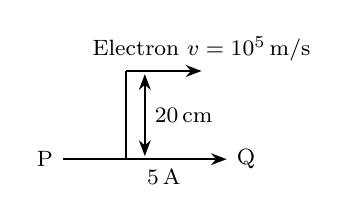
\begin{tikzpicture}[scale=0.8]
\draw[->] (0,0) node[left,lbl]{P} -- (2.6,0) node[right,lbl]{Q}; \node[lbl,below] at (1.6,0) {5\,A};
\draw (1,0) -- (1,1.4); \draw[->] (1,1.4) -- (2.2,1.4) node[above,lbl]{Electron $v = 10^5\unit{m/s}$};
\draw[<->] (1.3,0.05) -- (1.3,1.35) node[midway,right,lbl]{20\,cm};
\end{tikzpicture}}\ntag{A}{118}{leph104}{12}{}{Class XII Part 1 \textperiodcentered{} Ch 4}}
{\opt{$4\times10^{-20}\unit{N}$}{$8\pi\times10^{-20}\unit{N}$}{$4\pi\times10^{-20}\unit{N}$}{$8\times10^{-20}\unit{N}$}}
\numoptstrue
\QQ{\qsrc{2021}{37}In the product $\vec F = q(\vec v\times\vec B) = q\vec v\times(B\hat i+B\hat j+B_0\hat k)$. For $q = 1$ and $\vec v = 2\hat i+4\hat j+6\hat k$ and $\vec F = 4\hat i-20\hat j+12\hat k$. What will be the complete expression for $\vec B$?\ntag{A}{109}{leph104}{3}{}{Class XII Part 1 \textperiodcentered{} Ch 4}}
{\opt{$-8\hat i-8\hat j-6\hat k$}{$-6\hat i-6\hat j-8\hat k$}{$8\hat i+8\hat j-6\hat k$}{$6\hat i+6\hat j-8\hat k$}}
\numoptstrue
\QQ{\qsrc{2019}{3}Ionized hydrogen atoms and $\alpha$-particles with same momenta enters perpendicular to a constant magnetic field, B. The ratio of their radii of their paths $r_H:r_\alpha$ will be:\ntag{A}{112}{leph104}{6}{}{Class XII Part 1 \textperiodcentered{} Ch 4}}
{\opt{2:1}{1:2}{4:1}{1:4}}
\topichead{Force on a current-carrying conductor}{2}
\numoptstrue
\QQ{\qsrc{2023}{47}A wire carrying a current $I$ along the positive $x$-axis has length $L$. It is kept in a magnetic field $\vec B = (2\hat i+3\hat j-4\hat k)\unit{T}$. The magnitude of the magnetic force acting on the wire is:\ntag{D}{110}{leph104}{4}{ \textperiodcentered{} F=I l x B}{Class XII Part 1 \textperiodcentered{} Ch 4}}
{\opt{$\sqrt3\,IL$}{$3IL$}{$\sqrt5\,IL$}{$5IL$}}
\numoptstrue
\QQ{\qsrc{2018}{26}A metallic rod of mass per unit length $0.5\unit{kg\,m^{-1}}$ is lying horizontally on a smooth inclined plane which makes an angle of $30^\circ$ with the horizontal. The rod is not allowed to slide down by flowing a current through it when a magnetic field of induction $0.25\unit{T}$ is acting on it in the vertical direction. The current flowing in the rod to keep it stationary is\ntag{A}{111}{leph104}{5}{}{Class XII Part 1 \textperiodcentered{} Ch 4}}
{\opt{14.76\,A}{5.98\,A}{7.14\,A}{11.32\,A}}
\topichead{Biot-Savart law and magnetic fields}{3}
\numoptstrue
\QQ{\qsrc{2026}{11}A current $I_0$ flows through a metallic circular loop of radius $r$ as shown in the figure. Resistance of the segment ABC is half that of ADC. Magnitude of magnetic field at the centre O of the loop is:
\fig{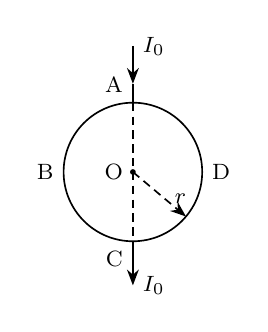
\begin{tikzpicture}[scale=0.8]
\draw (0,0) circle (1.1);
\draw[->] (0,2.0) -- (0,1.4) node[pos=0,right,lbl]{$I_0$}; \draw (0,1.4) -- (0,1.1);
\draw[->] (0,-1.1) -- (0,-1.8) node[right,lbl]{$I_0$};
\draw[densely dashed] (0,1.1) -- (0,-1.1); \draw[densely dashed,->] (0,0) -- (-40:1.1) node[pos=0.6,right,lbl]{$r$};
\fill (0,0) circle (1.3pt) node[left,lbl]{O};
\node[lbl,above left] at (0,1.1) {A}; \node[lbl,below left] at (0,-1.1) {C};
\node[lbl,left] at (-1.1,0) {B}; \node[lbl,right] at (1.1,0) {D};
\end{tikzpicture}}\ntag{A}{116}{leph104}{10}{}{Class XII Part 1 \textperiodcentered{} Ch 4}}
{\opt{$\dfrac{\mu_0I_0}{12r}$}{$\dfrac{\mu_0I_0}{4r}$}{$\dfrac{\mu_0I_0}{2r}$}{$\dfrac{\mu_0I_0}{2\pi r}$}}
\numoptstrue
\QQ{\qsrc{2024}{21}A tightly wound 100 turns coil of radius $10\unit{cm}$ carries a current of $7\unit{A}$. The magnitude of the magnetic field at the centre of the coil is (Take permeability of free space as $4\pi\times10^{-7}$ SI units):\ntag{D}{117}{leph104}{11}{ \textperiodcentered{} Example 4.6}{Class XII Part 1 \textperiodcentered{} Ch 4}}
{\opt{44\,T}{44\,mT}{4.4\,T}{4.4\,mT}}
\numoptstrue
\QQ{\qsrc{2022}{19}Given below are two statements:\par
\textbf{Statement I}: Biot-Savart's law gives us the expression for the magnetic field strength of an infinitesimal current element ($Idl$) of a current carrying conductor only.\par
\textbf{Statement II}: Biot-Savart's law is analogous to Coulomb's inverse square law of charge $q$, with the former being related to the field produced by a scalar source, $Idl$ while the latter being produced by a vector source, $q$.\par
In light of above statements choose the most appropriate answer from the options given below:\ntag{D}{114}{leph104}{8}{ \textperiodcentered{} Biot-Savart law}{Class XII Part 1 \textperiodcentered{} Ch 4}}
{\opt{Statement I is incorrect and Statement II is correct}{Both Statement I and Statement II are correct}{Both Statement I and Statement II are incorrect}{Statement I is correct and Statement II is incorrect}}
\topichead{Ampere's law and solenoid}{6}
\numoptstrue
\QQ{\qsrc{2022}{35}A long solenoid of radius $1\unit{mm}$ has 100 turns per mm. If $1\unit{A}$ current flows in the solenoid, the magnetic field strength at the centre of the solenoid is:\ntag{D}{121}{leph104}{15}{ \textperiodcentered{} B=mu0 n I}{Class XII Part 1 \textperiodcentered{} Ch 4}}
{\opt{$6.28\times10^{-4}\unit{T}$}{$6.28\times10^{-2}\unit{T}$}{$12.56\times10^{-2}\unit{T}$}{$12.56\times10^{-4}\unit{T}$}}
\numoptstrue
\QQ{\qsrc{2022}{42}From Ampere's circuital law for a long straight wire of circular cross-section carrying a steady current, the variation of magnetic field in the inside and outside region of the wire is:\ntag{D}{119}{leph104}{13}{ \textperiodcentered{} Example 4.7}{Class XII Part 1 \textperiodcentered{} Ch 4}}
{\opt{a linearly decreasing function of distance upto the boundary of the wire and then a linearly increasing one for the outside region.}{uniform and remains constant for both the regions.}{a linearly increasing function of distance upto the boundary of the wire and then linearly decreasing for the outside region.}{a linearly increasing function of distance $r$ upto the boundary of the wire and then decreasing one with $1/r$ dependence for the outside region.}}
\numoptstrue
\QQ{\qsrc{2021}{26}A thick current carrying cable of radius `$R$' carries current `$I$' uniformly distributed across its cross-section. The variation of magnetic field $B(r)$ due to the cable with the distance `$r$' from the axis of the cable is represented by:\ntag{D}{119}{leph104}{13}{ \textperiodcentered{} Example 4.7}{Class XII Part 1 \textperiodcentered{} Ch 4}}
{\optfig{\gaxes{$r$}{$B$}{\draw (0,0) .. controls (1.0,0.1) and (1.6,0.5) .. (1.8,1.7);}}
{\gaxes{$r$}{$B$}{\draw (0,0) -- (1.7,1.5);}}
{\gaxes{$r$}{$B$}{\draw (0,0) -- (0.6,1.3) .. controls (1.0,0.6) and (1.3,0.35) .. (1.9,0.3); \draw[densely dashed] (0.6,1.3) -- (0.6,0);}}
{\gaxes{$r$}{$B$}{\draw (0,0) .. controls (0.2,1.0) and (0.6,1.4) .. (1.8,1.45);}}}
\numoptstrue
\QQ{\qsrc{2020}{172}A long solenoid of $50\unit{cm}$ length having 100 turns carries a current of $2.5\unit{A}$. The magnetic field at the centre of the solenoid is: ($\mu_0 = 4\pi\times10^{-7}\unit{T\,m\,A^{-1}}$)\ntag{D}{121}{leph104}{15}{ \textperiodcentered{} B=mu0 n I}{Class XII Part 1 \textperiodcentered{} Ch 4}}
{\opt{$6.28\times10^{-4}\unit{T}$}{$3.14\times10^{-4}\unit{T}$}{$6.28\times10^{-5}\unit{T}$}{$3.14\times10^{-5}\unit{T}$}}
\numoptstrue
\QQ{\qsrc{2019}{45}A cylindrical conductor of radius $R$ is carrying a constant current. The plot of the magnitude of the magnetic field, $B$ with the distance, $d$, from the centre of the conductor, is \textbf{correctly} represented by the figure:\ntag{D}{119}{leph104}{13}{ \textperiodcentered{} Example 4.7}{Class XII Part 1 \textperiodcentered{} Ch 4}}
{\optfig{\gaxes{$d$}{$B$}{\draw (0,1.3) -- (0.8,1.3) .. controls (1.1,0.7) and (1.4,0.4) .. (1.8,0.3); \draw[densely dashed] (0.8,1.3) -- (0.8,0) node[below,font=\tiny]{$R$};}}
{\gaxes{$d$}{$B$}{\draw (0.8,1.3) .. controls (1.1,0.7) and (1.4,0.4) .. (1.8,0.3); \draw (0.8,1.3) -- (0.8,0) node[below,font=\tiny]{$R$};}}
{\gaxes{$d$}{$B$}{\draw (0,0) -- (0.8,1.3) .. controls (1.1,0.7) and (1.4,0.4) .. (1.8,0.3); \draw[densely dashed] (0.8,1.3) -- (0.8,0) node[below,font=\tiny]{$R$};}}
{\gaxes{$d$}{$B$}{\draw (0,0) -- (0.8,1.3) -- (1.8,1.3); \draw[densely dashed] (0.8,1.3) -- (0.8,0) node[below,font=\tiny]{$R$};}}}
\numoptstrue
\QQ{\qsrc{2016}{26}A long straight wire of radius $a$ carries a steady current $I$. The current is uniformly distributed over its cross-section. The ratio of the magnetic fields $B$ and $B'$, at radial distances $\dfrac a2$ and $2a$ respectively, from the axis of the wire is:\ntag{D}{119}{leph104}{13}{ \textperiodcentered{} Example 4.7}{Class XII Part 1 \textperiodcentered{} Ch 4}}
{\opt{$\dfrac14$}{$\dfrac12$}{1}{4}}
\topichead{Force between parallel currents}{3}
\numoptstrue
\QQ{\qsrc{2026}{15}Two infinitely long parallel conducting wires A and B carry currents $I$ and $2I$, respectively, in the same direction. The wire A has uniform mass per unit length $\lambda$ and lies on an insulated floor. The wire B is kept fixed at a height $h$ above the floor. The minimum magnitude of $h$ so that the wire A does not rise from the floor is: [$g$ is the acceleration due to gravity and $\mu_0$ is the permeability of free space.]\ntag{A}{123}{leph104}{17}{}{Class XII Part 1 \textperiodcentered{} Ch 4}}
{\opt{$\dfrac{\mu_0I^2}{2\pi\lambda g}$}{$\dfrac{\mu_0I^2}{\pi\lambda g}$}{$\dfrac{2\mu_0I^2}{\pi\lambda g}$}{$\dfrac{4\mu_0I^2}{\pi\lambda g}$}}
\numoptstrue
\QQ{\qsrc{2017}{139}An arrangement of three parallel straight wires placed perpendicular to plane of paper carrying same current `$I$' along the same direction is shown in Fig. Magnitude of force per unit length on the middle wire `B' is given by:
\fig{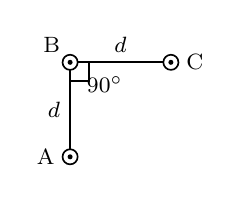
\begin{tikzpicture}[scale=0.8]
\draw (0,1.5) circle (0.12) node[above left,lbl]{B}; \fill (0,1.5) circle (0.04); \draw (1.6,1.5) circle (0.12) node[right=2pt,lbl]{C}; \fill (1.6,1.5) circle (0.04); \draw (0,0) circle (0.12) node[left=2pt,lbl]{A}; \fill (0,0) circle (0.04);
\draw (0.12,1.5) -- (1.48,1.5) node[midway,above,lbl]{$d$}; \draw (0,1.38) -- (0,0.12) node[midway,left,lbl]{$d$}; \draw (0,1.2) -- (0.3,1.2) -- (0.3,1.5); \node[lbl] at (0.55,1.15) {$90^\circ$};
\end{tikzpicture}}\ntag{A}{123}{leph104}{17}{}{Class XII Part 1 \textperiodcentered{} Ch 4}}
{\opt{$\dfrac{2\mu_0i^2}{\pi d}$}{$\dfrac{\sqrt2\mu_0i^2}{\pi d}$}{$\dfrac{\mu_0i^2}{\sqrt2\pi d}$}{$\dfrac{\mu_0i^2}{2\pi d}$}}
\numoptstrue
\QQ{\qsrc{2016}{2}A square loop ABCD carrying a current $i$, is placed near and coplanar with a long straight conductor XY carrying a current $I$, the net force on the loop will be:
\fig{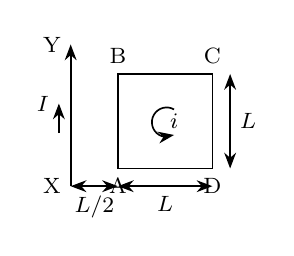
\begin{tikzpicture}[scale=0.75]
\draw[->] (0,0) -- (0,2.4) node[left,lbl]{Y}; \node[lbl,left] at (0,0) {X}; \draw[->] (-0.2,0.9) -- (-0.2,1.4) node[left,lbl]{$I$};
\draw (0.8,0.3) rectangle (2.4,1.9); \node[lbl,below] at (0.8,0.3) {A}; \node[lbl,above] at (0.8,1.9) {B}; \node[lbl,above] at (2.4,1.9) {C}; \node[lbl,below] at (2.4,0.3) {D};
\draw[->] (1.75,1.3) arc (60:300:0.25); \node[lbl] at (1.75,1.1) {$i$};
\draw[<->] (0,0.0) -- (0.8,0.0) node[midway,below,lbl]{$L/2$}; \draw[<->] (0.8,0.0) -- (2.4,0.0) node[midway,below,lbl]{$L$}; \draw[<->] (2.7,0.3) -- (2.7,1.9) node[midway,right,lbl]{$L$};
\end{tikzpicture}}\ntag{A}{123}{leph104}{17}{ \textperiodcentered{} force between parallel currents}{Class XII Part 1 \textperiodcentered{} Ch 4}}
{\opt{$\dfrac{2\mu_0Ii}{3\pi}$}{$\dfrac{\mu_0Ii}{2\pi}$}{$\dfrac{2\mu_0IiL}{3\pi}$}{$\dfrac{\mu_0IiL}{2\pi}$}}
\topichead{Magnetic dipole and bar magnet}{2}
\numoptstrue
\QQ{\qsrc{2025}{12}A $2\unit{A}$ current is flowing through two different small circular copper coils having radii ratio $1:2$. The ratio of their respective magnetic moments will be\ntag{D}{125}{leph104}{19}{ \textperiodcentered{} m=NIA}{Class XII Part 1 \textperiodcentered{} Ch 4}}
{\opt{1:4}{1:2}{2:1}{4:1}}
\numoptstrue
\QQ{\qsrc{2021}{44}A uniform conducting wire of length $12a$ and resistance `$R$' is wound up as a current carrying coil in the shape of, (i) an equilateral triangle of side `$a$', (ii) a square of side `$a$'. The magnetic dipole moments of the coil in each case respectively are:\ntag{A}{125}{leph104}{19}{}{Class XII Part 1 \textperiodcentered{} Ch 4}}
{\opt{$\sqrt3Ia^2$ and $3Ia^2$}{$3Ia^2$ and $Ia^2$}{$3Ia^2$ and $4Ia^2$}{$4Ia^2$ and $3Ia^2$}}
\topichead{Moving coil galvanometer, ammeter, voltmeter}{1}
\numoptstrue
\QQ{\qsrc{2018}{29}Current sensitivity of a moving coil galvanometer is 5\,div/mA and its voltage sensitivity (angular deflection per unit voltage applied) is 20\,div/V. The resistance of the galvanometer is\ntag{D}{130}{leph104}{24}{ \textperiodcentered{} current and voltage sensitivity}{Class XII Part 1 \textperiodcentered{} Ch 4}}
{\opt{250\,$\Omega$}{25\,$\Omega$}{40\,$\Omega$}{500\,$\Omega$}}
\topichead{Dimensional analysis}{1}
\numoptstrue
\QQ{\qsrc{2022}{24}The dimensions $[\mathrm{MLT^{-2}A^{-2}}]$ belong to the:\ntag{D}{134}{leph104}{28}{ \textperiodcentered{} dimension table (mu0)}{Class XII Part 1 \textperiodcentered{} Ch 4}}
{\opt{electric permittivity}{magnetic flux}{self inductance}{magnetic permeability}}
\end{multicols}
\par\needspace{12\baselineskip}\vspace{12pt}
\begin{center}{\pgfornament[width=3.2cm,color=gilt]{87}}\par
{\large\color{navy}\scshape Moving Charges and Magnetism \textperiodcentered{} Answer Key}\end{center}
{\small\setlength{\tabcolsep}{1pt}\renewcommand{\arraystretch}{1.5}
\begin{tabularx}{\linewidth}{@{}*{8}{>{\centering\arraybackslash}X}@{}}\toprule
\textbf{1}\,(2) & \textbf{2}\,(4) & \textbf{3}\,(2) & \textbf{4}\,(1) & \textbf{5}\,(4) & \textbf{6}\,(4) & \textbf{7}\,(1) & \textbf{8}\,(4)\\
\textbf{9}\,(4) & \textbf{10}\,(3) & \textbf{11}\,(4) & \textbf{12}\,(3) & \textbf{13}\,(1) & \textbf{14}\,(3) & \textbf{15}\,(3) & \textbf{16}\,(2)\\
\textbf{17}\,(3) & \textbf{18}\,(1) & \textbf{19}\,(1) & \textbf{20}\,(1) & \textbf{21}\,(1) & \textbf{22}\,(4) &  & \\\bottomrule\end{tabularx}}\par\smallskip
{\footnotesize Answers of 2021, 2022, 2023, 2025 and 2026 are from the official NTA final keys (checked by the editor); answers of 2016--2020 and 2024 were solved by the editor.
}\par
\par\needspace{18\baselineskip}\vspace{14pt}
\begin{center}{\pgfornament[width=3.2cm,color=gilt]{87}}\par
{\large\color{navy}\scshape Chapter Summary \textperiodcentered{} Moving Charges and Magnetism}\end{center}
{\small\setlength{\tabcolsep}{3.5pt}
\begin{tabular*}{\linewidth}{@{\extracolsep{\fill}}l*{11}{c}c@{}}\toprule
Year & 2016 & 2017 & 2018 & 2019 & 2020 & 2021 & 2022 & 2023 & 2024 & 2025 & 2026 & Total\\\midrule
Questions & 2 & 1 & 2 & 2 & 1 & 4 & 4 & 1 & 1 & 2 & 2 & \textbf{22}\\\bottomrule\end{tabular*}}\par\medskip
{\small\textbf{\color{crimson}Topic-wise} (in textbook order)\par\smallskip
\begin{tabularx}{\linewidth}{@{}>{\raggedright\arraybackslash}Xrrrl@{}}\toprule
Topic & Qs & Direct & Years & 2016 $\rightarrow$ 2026\\\midrule
Charged particle in a magnetic field & \textbf{4} & 0 & 3 & {\scriptsize {\color{gray!45}16} {\color{gray!45}17} {\color{gray!45}18} \textbf{19} {\color{gray!45}20} \textbf{21} {\color{gray!45}22} {\color{gray!45}23} {\color{gray!45}24} \textbf{25} {\color{gray!45}26}}\\
Force on a current-carrying conductor & \textbf{2} & 1 & 2 & {\scriptsize {\color{gray!45}16} {\color{gray!45}17} \textbf{18} {\color{gray!45}19} {\color{gray!45}20} {\color{gray!45}21} {\color{gray!45}22} \textbf{23} {\color{gray!45}24} {\color{gray!45}25} {\color{gray!45}26}}\\
Biot-Savart law and magnetic fields & \textbf{3} & 2 & 3 & {\scriptsize {\color{gray!45}16} {\color{gray!45}17} {\color{gray!45}18} {\color{gray!45}19} {\color{gray!45}20} {\color{gray!45}21} \textbf{22} {\color{gray!45}23} \textbf{24} {\color{gray!45}25} \textbf{26}}\\
Ampere's law and solenoid & \textbf{6} & 6 & 5 & {\scriptsize \textbf{16} {\color{gray!45}17} {\color{gray!45}18} \textbf{19} \textbf{20} \textbf{21} \textbf{22} {\color{gray!45}23} {\color{gray!45}24} {\color{gray!45}25} {\color{gray!45}26}}\\
Force between parallel currents & \textbf{3} & 0 & 3 & {\scriptsize \textbf{16} \textbf{17} {\color{gray!45}18} {\color{gray!45}19} {\color{gray!45}20} {\color{gray!45}21} {\color{gray!45}22} {\color{gray!45}23} {\color{gray!45}24} {\color{gray!45}25} \textbf{26}}\\
Magnetic dipole and bar magnet & \textbf{2} & 1 & 2 & {\scriptsize {\color{gray!45}16} {\color{gray!45}17} {\color{gray!45}18} {\color{gray!45}19} {\color{gray!45}20} \textbf{21} {\color{gray!45}22} {\color{gray!45}23} {\color{gray!45}24} \textbf{25} {\color{gray!45}26}}\\
Moving coil galvanometer, ammeter, voltmeter & \textbf{1} & 1 & 1 & {\scriptsize {\color{gray!45}16} {\color{gray!45}17} \textbf{18} {\color{gray!45}19} {\color{gray!45}20} {\color{gray!45}21} {\color{gray!45}22} {\color{gray!45}23} {\color{gray!45}24} {\color{gray!45}25} {\color{gray!45}26}}\\
Dimensional analysis & \textbf{1} & 1 & 1 & {\scriptsize {\color{gray!45}16} {\color{gray!45}17} {\color{gray!45}18} {\color{gray!45}19} {\color{gray!45}20} {\color{gray!45}21} \textbf{22} {\color{gray!45}23} {\color{gray!45}24} {\color{gray!45}25} {\color{gray!45}26}}\\
\bottomrule\end{tabularx}}\par\medskip
\begin{minipage}[t]{0.34\linewidth}{\small\textbf{\color{crimson}Direct vs Applied}\par\smallskip
\begin{tabular}{@{}lrr@{}}\toprule
Direct from NCERT & \textbf{12} & 55\%\\
\quad text, table, figure & 7 &\\
\quad solved Example & 5 &\\
\quad Exercise & 0 &\\
Applied & \textbf{10} & 45\%\\\midrule
Easy / Mod. / Hard & \multicolumn{2}{r}{11 / 10 / 1}\\\bottomrule
\end{tabular}}\end{minipage}\hfill
\begin{minipage}[t]{0.63\linewidth}{\small\textbf{\color{crimson}What to focus on}\par\smallskip
\begin{itemize}[leftmargin=1.1em,itemsep=1pt,topsep=0pt]
\item 22 questions in 11 papers, about 2.0 per paper; rank 6 of 28 chapters by number of questions.
\item Most asked topic: \textbf{Ampere's law and solenoid} (6 questions, in 5 of the 11 years).
\item 5 questions are NCERT solved Examples or Exercises: Example 4.6 (Q 8), Example 4.7 (Q 11), Example 4.7 (Q 12), Example 4.7 (Q 14), Example 4.7 (Q 15). Work these by hand.
\item NCERT pages that gave three or more questions: page 119 (4 questions), page 123 (3 questions). Read these pages line by line.
\item Difficulty: 11 easy, 10 moderate, 1 hard (hard: Q 1).
\item 10 applied questions: practise these after the NCERT Examples and Exercises of the chapter.
\end{itemize}}\end{minipage}\par
\chapterpaper{Class XII \textperiodcentered{} Chapter 5}{Magnetism and Matter}{7 questions \textperiodcentered{} 3 topics \textperiodcentered{} NEET 2016--2026}{cleph105}{XII.5 Magnetism and Matter}
\begin{multicols}{2}
\topichead{Magnetic dipole and bar magnet}{2}
\numoptstrue
\QQ{\qsrc{2024}{47}An iron bar of length L has magnetic moment M. It is bent at the middle of its length such that the two arms make an angle $60^\circ$ with each other. The magnetic moment of this new magnet is:\ntag{A}{138}{leph105}{3}{}{Class XII Part 1 \textperiodcentered{} Ch 5}}
{\opt{$\dfrac M{\sqrt3}$}{M}{$\dfrac M2$}{2M}}
\numoptstrue
\QQ{\qsrc{2017}{148}A 250-turn rectangular coil of length $2.1\unit{cm}$ and width $1.25\unit{cm}$ carries a current of $85\unit{\mu A}$ and subjected to a magnetic field of strength $0.85\unit{T}$. Work done for rotating the coil by $180^\circ$ against the torque is:\ntag{A}{139}{leph105}{4}{ \textperiodcentered{} U=-m.B, W=2mB}{Class XII Part 1 \textperiodcentered{} Ch 5}}
{\opt{$4.55\unit{\mu J}$}{$2.3\unit{\mu J}$}{$1.15\unit{\mu J}$}{$9.1\unit{\mu J}$}}
\topichead{Magnetic field lines and Gauss's law for magnetism}{1}
\numoptstrue
\QQ{\qsrc{2023}{2}The net magnetic flux through any closed surface is:\ntag{D}{142}{leph105}{7}{ \textperiodcentered{} net flux through a closed surface is zero}{Class XII Part 1 \textperiodcentered{} Ch 5}}
{\opt{Negative}{Zero}{Positive}{Infinity}}
\topichead{Magnetic materials}{4}
\numoptstrue
\QQ{\qsrc{2024}{2}Match List-I with List-II.\par\smallskip
\begin{tabular}{@{}ll@{\ }lp{0.34\linewidth}@{}}
\multicolumn{2}{@{}l}{\textit{List-I} (Material)} & \multicolumn{2}{l}{\textit{List-II} (Susceptibility $\chi$)}\\
A. & Diamagnetic & I. & $\chi = 0$\\
B. & Ferromagnetic & II. & $0>\chi\ge-1$\\
C. & Paramagnetic & III. & $\chi\gg1$\\
D. & Non-magnetic & IV. & $0<\chi<\varepsilon$ (a small positive number)
\end{tabular}\par\smallskip
Choose the correct answer from the options given below:\ntag{D}{147}{leph105}{12}{ \textperiodcentered{} Table 5.2}{Class XII Part 1 \textperiodcentered{} Ch 5}}
{\opt{A-IV, B-III, C-II, D-I}{A-II, B-III, C-IV, D-I}{A-II, B-I, C-III, D-IV}{A-III, B-II, C-I, D-IV}}
\numoptstrue
\QQ{\qsrc{2020}{171}An iron rod of susceptibility 599 is subjected to a magnetising field of $1200\unit{A\,m^{-1}}$. The permeability of the material of the rod is: ($\mu_0 = 4\pi\times10^{-7}\unit{T\,m\,A^{-1}}$)\ntag{D}{146}{leph105}{11}{ \textperiodcentered{} mu=mu0(1+chi)}{Class XII Part 1 \textperiodcentered{} Ch 5}}
{\opt{$2.4\pi\times10^{-4}\unit{T\,m\,A^{-1}}$}{$8.0\times10^{-5}\unit{T\,m\,A^{-1}}$}{$2.4\pi\times10^{-5}\unit{T\,m\,A^{-1}}$}{$2.4\pi\times10^{-7}\unit{T\,m\,A^{-1}}$}}
\numoptstrue
\QQ{\qsrc{2018}{27}A thin diamagnetic rod is placed vertically between the poles of an electromagnet. When the current in the electromagnet is switched on, then the diamagnetic rod is pushed up, out of the horizontal magnetic field. Hence the rod gains gravitational potential energy. The work required to do this comes from\ntag{A}{147}{leph105}{12}{}{Class XII Part 1 \textperiodcentered{} Ch 5}}
{\opt{the lattice structure of the material of the rod}{the magnetic field}{the current source}{the induced electric field due to the changing magnetic field}}
\numoptstrue
\QQ{\qsrc{2016}{3}The magnetic susceptibility is negative for:\ntag{D}{147}{leph105}{12}{ \textperiodcentered{} diamagnetic: chi negative}{Class XII Part 1 \textperiodcentered{} Ch 5}}
{\opt{diamagnetic material only}{paramagnetic material only}{ferromagnetic material only}{paramagnetic and ferromagnetic materials}}
\end{multicols}
\par\needspace{12\baselineskip}\vspace{12pt}
\begin{center}{\pgfornament[width=3.2cm,color=gilt]{87}}\par
{\large\color{navy}\scshape Magnetism and Matter \textperiodcentered{} Answer Key}\end{center}
{\small\setlength{\tabcolsep}{1pt}\renewcommand{\arraystretch}{1.5}
\begin{tabularx}{\linewidth}{@{}*{8}{>{\centering\arraybackslash}X}@{}}\toprule
\textbf{1}\,(3) & \textbf{2}\,(4) & \textbf{3}\,(2) & \textbf{4}\,(2) & \textbf{5}\,(1) & \textbf{6}\,(3) & \textbf{7}\,(1) & \\\bottomrule\end{tabularx}}\par\smallskip
{\footnotesize Answers of 2021, 2022, 2023, 2025 and 2026 are from the official NTA final keys (checked by the editor); answers of 2016--2020 and 2024 were solved by the editor.
}\par
\par\needspace{18\baselineskip}\vspace{14pt}
\begin{center}{\pgfornament[width=3.2cm,color=gilt]{87}}\par
{\large\color{navy}\scshape Chapter Summary \textperiodcentered{} Magnetism and Matter}\end{center}
{\small\setlength{\tabcolsep}{3.5pt}
\begin{tabular*}{\linewidth}{@{\extracolsep{\fill}}l*{11}{c}c@{}}\toprule
Year & 2016 & 2017 & 2018 & 2019 & 2020 & 2021 & 2022 & 2023 & 2024 & 2025 & 2026 & Total\\\midrule
Questions & 1 & 1 & 1 & 0 & 1 & 0 & 0 & 1 & 2 & 0 & 0 & \textbf{7}\\\bottomrule\end{tabular*}}\par\medskip
{\small\textbf{\color{crimson}Topic-wise} (in textbook order)\par\smallskip
\begin{tabularx}{\linewidth}{@{}>{\raggedright\arraybackslash}Xrrrl@{}}\toprule
Topic & Qs & Direct & Years & 2016 $\rightarrow$ 2026\\\midrule
Magnetic dipole and bar magnet & \textbf{2} & 0 & 2 & {\scriptsize {\color{gray!45}16} \textbf{17} {\color{gray!45}18} {\color{gray!45}19} {\color{gray!45}20} {\color{gray!45}21} {\color{gray!45}22} {\color{gray!45}23} \textbf{24} {\color{gray!45}25} {\color{gray!45}26}}\\
Magnetic field lines and Gauss's law for magnetism & \textbf{1} & 1 & 1 & {\scriptsize {\color{gray!45}16} {\color{gray!45}17} {\color{gray!45}18} {\color{gray!45}19} {\color{gray!45}20} {\color{gray!45}21} {\color{gray!45}22} \textbf{23} {\color{gray!45}24} {\color{gray!45}25} {\color{gray!45}26}}\\
Magnetic materials & \textbf{4} & 3 & 4 & {\scriptsize \textbf{16} {\color{gray!45}17} \textbf{18} {\color{gray!45}19} \textbf{20} {\color{gray!45}21} {\color{gray!45}22} {\color{gray!45}23} \textbf{24} {\color{gray!45}25} {\color{gray!45}26}}\\
\bottomrule\end{tabularx}}\par\medskip
\begin{minipage}[t]{0.34\linewidth}{\small\textbf{\color{crimson}Direct vs Applied}\par\smallskip
\begin{tabular}{@{}lrr@{}}\toprule
Direct from NCERT & \textbf{4} & 57\%\\
\quad text, table, figure & 4 &\\
\quad solved Example & 0 &\\
\quad Exercise & 0 &\\
Applied & \textbf{3} & 43\%\\\midrule
Easy / Mod. / Hard & \multicolumn{2}{r}{4 / 3 / 0}\\\bottomrule
\end{tabular}}\end{minipage}\hfill
\begin{minipage}[t]{0.63\linewidth}{\small\textbf{\color{crimson}What to focus on}\par\smallskip
\begin{itemize}[leftmargin=1.1em,itemsep=1pt,topsep=0pt]
\item 7 questions in 11 papers, about 0.6 per paper; rank 27 of 28 chapters by number of questions.
\item Most asked topic: \textbf{Magnetic materials} (4 questions, in 4 of the 11 years).
\item NCERT pages that gave three or more questions: page 147 (3 questions). Read these pages line by line.
\item Difficulty: 4 easy, 3 moderate, 0 hard.
\item 3 applied questions: practise these after the NCERT Examples and Exercises of the chapter.
\end{itemize}}\end{minipage}\par
\chapterpaper{Class XII \textperiodcentered{} Chapter 6}{Electromagnetic Induction}{15 questions \textperiodcentered{} 3 topics \textperiodcentered{} NEET 2016--2026}{cleph106}{XII.6 Electromagnetic Induction}
\begin{multicols}{2}
\topichead{Magnetic flux}{1}
\numoptstrue
\QQ{\qsrc{2022}{33}A square loop of side $1\unit{m}$ and resistance $1\unit{\Omega}$ is placed in a magnetic field of $0.5\unit{T}$. If the plane of loop is perpendicular to the direction of magnetic field, the magnetic flux through the loop is:\ntag{D}{156}{leph106}{3}{ \textperiodcentered{} Phi=BA}{Class XII Part 1 \textperiodcentered{} Ch 6}}
{\opt{zero weber}{2 weber}{0.5 weber}{1 weber}}
\topichead{Faraday's law and Lenz's law}{6}
\numoptstrue
\QQ{\qsrc{2026}{32}A conducting loop of finite resistance lies on the $x$--$y$ plane. There is a constant magnetic field in the $z$ direction. The area of the loop varies with time $t$, as $A = A_0(1+\sin t)$ in appropriate units. The figure that correctly indicates the qualitative behaviour of the power $P$ dissipated in the loop as a function of time is:\ntag{A}{157}{leph106}{4}{}{Class XII Part 1 \textperiodcentered{} Ch 6}}
{\optfig{\gaxes{$t$}{$P$}{\draw (0,0) .. controls (0.1,1.4) and (0.7,1.4) .. (0.8,0) .. controls (0.9,1.4) and (1.5,1.4) .. (1.6,0); \node[font=\tiny,below] at (0,0) {0};}}
{\gaxes{$t$}{$P$}{\draw (0,1.3) .. controls (0.2,0.4) and (0.6,0.05) .. (0.8,0) .. controls (1.0,0.05) and (1.4,0.4) .. (1.6,1.3); \node[font=\tiny,below] at (0,0) {0};}}
{\gaxes{$t$}{$P$}{\draw (0,1.2) -- (1.8,1.2); \node[font=\tiny,below] at (0,0) {0};}}
{\gaxes{$t$}{$P$}{\draw (0,0) .. controls (0.9,0.1) and (1.4,0.5) .. (1.8,1.5); \node[font=\tiny,below] at (0,0) {0};}}}
\numoptstrue
\QQ{\qsrc{2024}{19}\fig{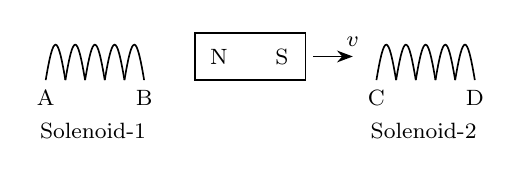
\begin{tikzpicture}[scale=1.0]
\foreach \x in {0,0.25,...,1.0} \draw (\x,0) .. controls (\x+0.1,0.6) and (\x+0.15,0.6) .. (\x+0.25,0);
\node[lbl,below] at (0,0) {A}; \node[lbl,below] at (1.25,0) {B}; \node[lbl] at (0.6,-0.65) {Solenoid-1};
\draw (1.9,0) rectangle (3.3,0.6); \node[lbl] at (2.2,0.3) {N}; \node[lbl] at (3.0,0.3) {S};
\draw[->] (3.4,0.3) -- (3.9,0.3) node[above,lbl]{$v$};
\begin{scope}[xshift=4.2cm]
\foreach \x in {0,0.25,...,1.0} \draw (\x,0) .. controls (\x+0.1,0.6) and (\x+0.15,0.6) .. (\x+0.25,0);
\node[lbl,below] at (0,0) {C}; \node[lbl,below] at (1.25,0) {D}; \node[lbl] at (0.6,-0.65) {Solenoid-2};
\end{scope}
\end{tikzpicture}}
In the above diagram, a strong bar magnet is moving towards solenoid-2 from solenoid-1. The direction of induced current in solenoid-1 and that in solenoid-2, respectively, are through the directions:\ntag{A}{160}{leph106}{7}{}{Class XII Part 1 \textperiodcentered{} Ch 6}}
{\opt{BA and DC}{AB and DC}{BA and CD}{AB and CD}}
\numoptstrue
\QQ{\qsrc{2024}{44}A sheet is placed on a horizontal surface in front of a strong magnetic pole. A force is needed to:
\begin{stmts}[\Alph*.]
\item hold the sheet there if it is magnetic.
\item hold the sheet there if it is non-magnetic.
\item move the sheet away from the pole with uniform velocity if it is conducting.
\item move the sheet away from the pole with uniform velocity if it is both, non-conducting and non-polar.
\end{stmts}
Choose the correct statement(s) from the options given below:\ntag{A}{160}{leph106}{7}{}{Class XII Part 1 \textperiodcentered{} Ch 6}}
{\opt{C only}{B and D only}{A and C only}{A, C and D only}}
\numoptstrue
\QQ{\qsrc{2022}{48}A big circular coil of 1000 turns and average radius $10\unit{m}$ is rotating about its horizontal diameter at $2\unit{rad\,s^{-1}}$. If the vertical component of earth's magnetic field at that place is $2\times10^{-5}\unit{T}$ and electrical resistance of the coil is $12.56\unit{\Omega}$, then the maximum induced current in the coil will be:\ntag{A}{171}{leph106}{18}{}{Class XII Part 1 \textperiodcentered{} Ch 6}}
{\opt{2\,A}{0.25\,A}{1.5\,A}{1\,A}}
\numoptstrue
\QQ{\qsrc{2019}{41}A 800 turn coil of effective area $0.05\unit{m^2}$ is kept perpendicular to a magnetic field $5\times10^{-5}\unit{T}$. When the plane of the coil is rotated by $90^\circ$ around any of its coplanar axis in $0.1\unit{s}$, the emf induced in the coil will be:\ntag{D}{158}{leph106}{5}{ \textperiodcentered{} emf = -N dPhi/dt}{Class XII Part 1 \textperiodcentered{} Ch 6}}
{\opt{2\,V}{0.2\,V}{$2\times10^{-3}$\,V}{0.02\,V}}
\numoptstrue
\QQ{\qsrc{2017}{179}A long solenoid of diameter $0.1\unit{m}$ has $2\times10^4$ turns per meter. At the centre of the solenoid, a coil of 100 turns and radius $0.01\unit{m}$ is placed with its axis coinciding with the solenoid axis. The current in the solenoid reduces at a constant rate to 0\,A from 4\,A in $0.05\unit{s}$. If the resistance of the coil is $10\pi^2\unit{\Omega}$, the total charge flowing through the coil during this time is:\ntag{A}{157}{leph106}{4}{ \textperiodcentered{} Q = N delta-phi / R}{Class XII Part 1 \textperiodcentered{} Ch 6}}
{\opt{$16\unit{\mu C}$}{$32\unit{\mu C}$}{$16\pi\unit{\mu C}$}{$32\pi\unit{\mu C}$}}
\topichead{Self and mutual inductance}{8}
\numoptstrue
\QQ{\qsrc{2026}{3}Two identical inductors are connected in two different configurations P and Q, where a time varying current $I(t)$ is flowing, as shown in the figure. The induced emf between points $a$ and $b$ for configuration P is $E_P$ and that for configuration Q is $E_Q$. The ratio $E_P/E_Q$ is: [Neglect the effect of mutual inductance.]
\fig{\begin{circuitikz}[scale=0.62,transform shape,font=\Large]
\draw[->] (0,4.6) node[above]{$I(t)$} -- (0,4.1);
\draw (0,4.1) -- (0,3.8) node[circ]{} node[right]{$a$} to[L] (0,2.2) node[circ]{} node[right]{$b$} to[L] (0,0.6) -- (0,0.2);
\node at (0,-0.3) {(P)};
\draw[->] (3.6,4.6) node[above]{$I(t)$} -- (3.6,4.1);
\draw (3.6,4.1) -- (3.6,3.8) node[circ]{} node[right]{$a$};
\draw (2.9,3.8) -- (4.3,3.8); \draw (2.9,3.8) to[L] (2.9,1.6); \draw (4.3,3.8) to[L] (4.3,1.6);
\draw (2.9,1.6) -- (4.3,1.6); \draw (3.6,1.6) node[circ]{} node[below right]{$b$} -- (3.6,1.0);
\node at (3.6,-0.3) {(Q)};
\end{circuitikz}}\ntag{A}{168}{leph106}{15}{}{Class XII Part 1 \textperiodcentered{} Ch 6}}
{\opt{$\dfrac14$}{$\dfrac12$}{1}{2}}
\numoptstrue
\QQ{\qsrc{2026}{5}Consider a long solenoid of length $l$ and radius $r$. If $n$ is the number of turns per unit length and $\mu_0$ is the permeability of free space, the inductance of the solenoid is:\ntag{D}{168}{leph106}{15}{ \textperiodcentered{} L=mu0 n\textasciicircum{}2 A l}{Class XII Part 1 \textperiodcentered{} Ch 6}}
{\opt{$\mu_0\pi n^2r^2l$}{$\mu_0n^2r^2l$}{$(\mu_0/2\pi)n^2r^2l$}{$2\mu_0\pi n^2r^2l$}}
\numoptstrue
\QQ{\qsrc{2025}{11}AB is a part of an electrical circuit (see figure). The potential difference $V_A-V_B$, at the instant when current $i = 2\unit{A}$ and is increasing at a rate of $1\unit{A}$ per second is:
\fig{\begin{circuitikz}[scale=0.62,transform shape,font=\Large]
\draw (0,0) node[circ]{} node[left]{A} to[short,i=$i$] (1.0,0) to[L,l_=1\,H] (3.0,0) -- (3.7,0) (3.9,0) -- (4.6,0) to[R,l_=2\,$\Omega$] (6.6,0) node[circ]{} node[right]{B};
\draw (3.7,0.45) -- (3.7,-0.45); \draw[line width=2pt] (3.9,0.22) -- (3.9,-0.22); \node at (3.8,-0.85) {5\,V};
\end{circuitikz}}\ntag{A}{168}{leph106}{15}{}{Class XII Part 1 \textperiodcentered{} Ch 6}}
{\opt{5 volt}{6 volt}{9 volt}{10 volt}}
\numoptstrue
\QQ{\qsrc{2023}{19}The magnetic energy stored in an inductor of inductance $4\unit{\mu H}$ carrying a current of $2\unit{A}$ is:\ntag{D}{169}{leph106}{16}{ \textperiodcentered{} U=LI\textasciicircum{}2/2}{Class XII Part 1 \textperiodcentered{} Ch 6}}
{\opt{$8\unit{\mu J}$}{$4\unit{\mu J}$}{4\,mJ}{8\,mJ}}
\numoptstrue
\QQ{\qsrc{2021}{36}Two conducting circular loops of radii $R_1$ and $R_2$ are placed in the same plane with their centres coinciding. If $R_1\gg R_2$, the mutual inductance M between them will be directly proportional to:\ntag{D}{167}{leph106}{14}{ \textperiodcentered{} Example 6.8}{Class XII Part 1 \textperiodcentered{} Ch 6}}
{\opt{$\dfrac{R_1}{R_2}$}{$\dfrac{R_2}{R_1}$}{$\dfrac{R_1^2}{R_2}$}{$\dfrac{R_2^2}{R_1}$}}
\numoptstrue
\QQ{\qsrc{2018}{21}The magnetic potential energy stored in a certain inductor is $25\unit{mJ}$, when the current in the inductor is $60\unit{mA}$. This inductor is of inductance\ntag{D}{169}{leph106}{16}{ \textperiodcentered{} U=LI\textasciicircum{}2/2}{Class XII Part 1 \textperiodcentered{} Ch 6}}
{\opt{1.389\,H}{138.88\,H}{0.138\,H}{13.89\,H}}
\numoptstrue
\QQ{\qsrc{2017}{159}Figure shows a circuit that contains three identical resistors with resistance $R = 9.0\unit{\Omega}$ each, two identical inductors with inductance $L = 2.0\unit{mH}$ each, and an ideal battery with emf $\varepsilon = 18\unit{V}$. The current `$i$' through the battery just after the switch closed is,
\fig{\begin{circuitikz}[scale=0.55,transform shape,font=\Large]
\draw (0,0) to[battery1,l=$\varepsilon$,invert] (0,3) -- (6,3);
\draw (2,3) to[L,l_=L] (2,1.5) to[R,l_=R] (2,0); \draw (4,3) to[R,l=R] (4,0); \draw (6,3) to[R,l=R] (6,1.5) to[L,l_=L] (6,0);
\draw (6,1.5) -- (7.5,1.5) to[C,l=C] (7.5,0) -- (6,0);
\draw (0,0) to[nos] (2,0) -- (6,0);
\end{circuitikz}}\ntag{A}{167}{leph106}{14}{ \textperiodcentered{} inductor opposes sudden change}{Class XII Part 1 \textperiodcentered{} Ch 6}}
{\opt{0.2\,A}{2\,A}{0 ampere}{2\,mA}}
\numoptstrue
\QQ{\qsrc{2016}{42}A long solenoid has 1000 turns. When a current of 4\,A flows through it, the magnetic flux linked with each turn of the solenoid is $4\times10^{-3}\unit{Wb}$. The self-inductance of the solenoid is:\ntag{D}{167}{leph106}{14}{ \textperiodcentered{} N Phi = L I}{Class XII Part 1 \textperiodcentered{} Ch 6}}
{\opt{4\,H}{3\,H}{2\,H}{1\,H}}
\end{multicols}
\par\needspace{12\baselineskip}\vspace{12pt}
\begin{center}{\pgfornament[width=3.2cm,color=gilt]{87}}\par
{\large\color{navy}\scshape Electromagnetic Induction \textperiodcentered{} Answer Key}\end{center}
{\small\setlength{\tabcolsep}{1pt}\renewcommand{\arraystretch}{1.5}
\begin{tabularx}{\linewidth}{@{}*{8}{>{\centering\arraybackslash}X}@{}}\toprule
\textbf{1}\,(3) & \textbf{2}\,(2) & \textbf{3}\,(2)$^{*}$ & \textbf{4}\,(3) & \textbf{5}\,(4) & \textbf{6}\,(4) & \textbf{7}\,(2) & \textbf{8}\,(4)\\
\textbf{9}\,(1) & \textbf{10}\,(4) & \textbf{11}\,(1) & \textbf{12}\,(4) & \textbf{13}\,(4) & \textbf{14}\,(2)$^{*}$ & \textbf{15}\,(4) & \\\bottomrule\end{tabularx}}\par\smallskip
{\footnotesize Answers of 2021, 2022, 2023, 2025 and 2026 are from the official NTA final keys (checked by the editor); answers of 2016--2020 and 2024 were solved by the editor. $^{*}$: see note.
\par\smallskip\textbf{3.} (NEET 2024 Q19) By Lenz's law, solenoid-1 (N pole receding) and solenoid-2 (S pole approaching) both oppose the change; with the winding shown this gives A to B and D to C.
\par\smallskip\textbf{14.} (NEET 2017 Q159) The capacitor in the printed figure is not mentioned in the question; with only the three resistors and two inductors, just the middle resistor carries current at $t=0$: $i=18/9=2$\,A.
}\par
\par\needspace{18\baselineskip}\vspace{14pt}
\begin{center}{\pgfornament[width=3.2cm,color=gilt]{87}}\par
{\large\color{navy}\scshape Chapter Summary \textperiodcentered{} Electromagnetic Induction}\end{center}
{\small\setlength{\tabcolsep}{3.5pt}
\begin{tabular*}{\linewidth}{@{\extracolsep{\fill}}l*{11}{c}c@{}}\toprule
Year & 2016 & 2017 & 2018 & 2019 & 2020 & 2021 & 2022 & 2023 & 2024 & 2025 & 2026 & Total\\\midrule
Questions & 1 & 2 & 1 & 1 & 0 & 1 & 2 & 1 & 2 & 1 & 3 & \textbf{15}\\\bottomrule\end{tabular*}}\par\medskip
{\small\textbf{\color{crimson}Topic-wise} (in textbook order)\par\smallskip
\begin{tabularx}{\linewidth}{@{}>{\raggedright\arraybackslash}Xrrrl@{}}\toprule
Topic & Qs & Direct & Years & 2016 $\rightarrow$ 2026\\\midrule
Magnetic flux & \textbf{1} & 1 & 1 & {\scriptsize {\color{gray!45}16} {\color{gray!45}17} {\color{gray!45}18} {\color{gray!45}19} {\color{gray!45}20} {\color{gray!45}21} \textbf{22} {\color{gray!45}23} {\color{gray!45}24} {\color{gray!45}25} {\color{gray!45}26}}\\
Faraday's law and Lenz's law & \textbf{6} & 1 & 5 & {\scriptsize {\color{gray!45}16} \textbf{17} {\color{gray!45}18} \textbf{19} {\color{gray!45}20} {\color{gray!45}21} \textbf{22} {\color{gray!45}23} \textbf{24} {\color{gray!45}25} \textbf{26}}\\
Self and mutual inductance & \textbf{8} & 5 & 7 & {\scriptsize \textbf{16} \textbf{17} \textbf{18} {\color{gray!45}19} {\color{gray!45}20} \textbf{21} {\color{gray!45}22} \textbf{23} {\color{gray!45}24} \textbf{25} \textbf{26}}\\
\bottomrule\end{tabularx}}\par\medskip
\begin{minipage}[t]{0.34\linewidth}{\small\textbf{\color{crimson}Direct vs Applied}\par\smallskip
\begin{tabular}{@{}lrr@{}}\toprule
Direct from NCERT & \textbf{7} & 47\%\\
\quad text, table, figure & 6 &\\
\quad solved Example & 1 &\\
\quad Exercise & 0 &\\
Applied & \textbf{8} & 53\%\\\midrule
Easy / Mod. / Hard & \multicolumn{2}{r}{7 / 7 / 1}\\\bottomrule
\end{tabular}}\end{minipage}\hfill
\begin{minipage}[t]{0.63\linewidth}{\small\textbf{\color{crimson}What to focus on}\par\smallskip
\begin{itemize}[leftmargin=1.1em,itemsep=1pt,topsep=0pt]
\item 15 questions in 11 papers, about 1.4 per paper; rank 17 of 28 chapters by number of questions.
\item Most asked topic: \textbf{Self and mutual inductance} (8 questions, in 7 of the 11 years).
\item 1 questions are NCERT solved Examples or Exercises: Example 6.8 (Q 12). Work these by hand.
\item NCERT pages that gave three or more questions: page 168 (3 questions), page 167 (3 questions). Read these pages line by line.
\item Difficulty: 7 easy, 7 moderate, 1 hard (hard: Q 7).
\item 8 applied questions: practise these after the NCERT Examples and Exercises of the chapter.
\end{itemize}}\end{minipage}\par
\chapterpaper{Class XII \textperiodcentered{} Chapter 7}{Alternating Current}{17 questions \textperiodcentered{} 3 topics \textperiodcentered{} NEET 2016--2026}{cleph107}{XII.7 Alternating Current}
\begin{multicols}{2}
\topichead{AC power and rms values}{2}
\numoptstrue
\QQ{\qsrc{2022}{23}The peak voltage of the ac source is equal to:\ntag{D}{180}{leph107}{4}{ \textperiodcentered{} Vm=sqrt2 Vrms}{Class XII Part 1 \textperiodcentered{} Ch 7}}
{\opt{$1/\sqrt2$ times the rms value of the ac source}{the value of voltage supplied to the circuit}{the rms value of the ac source}{$\sqrt2$ times the rms value of the ac source}}
\numoptstrue
\QQ{\qsrc{2018}{28}An inductor $20\unit{mH}$, a capacitor $100\unit{\mu F}$ and a resistor $50\unit{\Omega}$ are connected in series across a source of emf, $V = 10\sin314t$. The power loss in the circuit is\ntag{A}{190}{leph107}{14}{}{Class XII Part 1 \textperiodcentered{} Ch 7}}
{\opt{2.74\,W}{0.43\,W}{0.79\,W}{1.13\,W}}
\topichead{AC circuits (reactance, LCR, phase)}{12}
\numoptstrue
\QQ{\qsrc{2026}{30}An ac voltage $V = 220\sin(2\times10^3t)$ volt is applied to a series LCR circuit. Then the current amplitude in this circuit is: (Given: $L = 10\unit{mH}$, $C = 25\unit{\mu F}$, $R = 100\unit{\Omega}$)\ntag{A}{188}{leph107}{12}{}{Class XII Part 1 \textperiodcentered{} Ch 7}}
{\opt{2.2\,A}{5.5\,A}{11.0\,A}{22.0\,A}}
\numoptstrue
\QQ{\qsrc{2025}{16}To an ac power supply of $220\unit{V}$ at $50\unit{Hz}$, a resistor of $20\unit{\Omega}$, a capacitor of reactance $25\unit{\Omega}$ and an inductor of reactance $45\unit{\Omega}$ are connected in series. The corresponding current in the circuit and the phase angle between the current and the voltage is, respectively\ntag{A}{187}{leph107}{11}{}{Class XII Part 1 \textperiodcentered{} Ch 7}}
{\opt{7.8\,A and $30^\circ$}{7.8\,A and $45^\circ$}{15.6\,A and $30^\circ$}{15.6\,A and $45^\circ$}}
\numoptstrue
\QQ{\qsrc{2024}{38}A $10\unit{\mu F}$ capacitor is connected to a $210\unit{V}$, $50\unit{Hz}$ source as shown in figure. The peak current in the circuit is nearly ($\pi = 3.14$):
\fig{\begin{circuitikz}[scale=0.6,transform shape,font=\Large]
\draw (0,0) to[sV] (0,1.8) -- (0,2.4) to[C,l={$C = 10\unit{\mu F}$}] (3,2.4) -- (3,0) -- (0,0); \node at (1.5,-0.5) {210\,V, 50\,Hz};
\end{circuitikz}}\ntag{D}{185}{leph107}{9}{ \textperiodcentered{} Example 7.4}{Class XII Part 1 \textperiodcentered{} Ch 7}}
{\opt{0.35\,A}{0.58\,A}{0.93\,A}{1.20\,A}}
\numoptstrue
\QQ{\qsrc{2023}{20}In a series LCR circuit, the inductance $L$ is $10\unit{mH}$, capacitance $C$ is $1\unit{\mu F}$ and resistance $R$ is $100\unit{\Omega}$. The frequency at which resonance occurs is:\ntag{D}{188}{leph107}{12}{ \textperiodcentered{} omega0=1/sqrt(LC)}{Class XII Part 1 \textperiodcentered{} Ch 7}}
{\opt{1.59\,kHz}{15.9\,rad/s}{15.9\,kHz}{1.59\,rad/s}}
\numoptstrue
\QQ{\qsrc{2023}{35}An ac source is connected to a capacitor C. Due to decrease in its operating frequency:\ntag{A}{185}{leph107}{9}{}{Class XII Part 1 \textperiodcentered{} Ch 7}}
{\opt{capacitive reactance remains constant}{capacitive reactance decreases.}{displacement current increases.}{displacement current decreases.}}
\numoptstrue
\QQ{\qsrc{2023}{38}The net impedance of circuit (as shown in figure) will be:
\fig{\begin{circuitikz}[scale=0.62,transform shape,font=\Large]
\draw (0,2) to[L,l_={$\frac{50}{\pi}$\,mH}] (2,2) to[C,l_={$\frac{10^3}{\pi}\,\mu$F}] (3.6,2) to[R,l=10\,$\Omega$] (5.4,2) -- (5.4,0) to[sV] (0,0) -- (0,2); \node at (2.7,-0.8) {220\,V, 50\,Hz};
\end{circuitikz}}\ntag{A}{187}{leph107}{11}{}{Class XII Part 1 \textperiodcentered{} Ch 7}}
{\opt{25\,$\Omega$}{$10\sqrt2$\,$\Omega$}{15\,$\Omega$}{$5\sqrt5$\,$\Omega$}}
\numoptstrue
\QQ{\qsrc{2022}{40}A series LCR circuit with inductance $10\unit{H}$, capacitance $10\unit{\mu F}$, resistance $50\unit{\Omega}$ is connected to an ac source of voltage, $V = 200\sin(100t)$ volt. If the resonant frequency of the LCR circuit is $\nu_0$ and the frequency of the ac source is $\nu$, then:\ntag{A}{188}{leph107}{12}{}{Class XII Part 1 \textperiodcentered{} Ch 7}}
{\opt{$\nu = 100\unit{Hz}$; $\nu_0 = \dfrac{100}\pi\unit{Hz}$}{$\nu_0 = \nu = 50\unit{Hz}$}{$\nu_0 = \nu = \dfrac{50}\pi\unit{Hz}$}{$\nu_0 = \dfrac{50}\pi\unit{Hz}$, $\nu = 50\unit{Hz}$}}
\numoptstrue
\QQ{\qsrc{2021}{20}An inductor of inductance $L$, a capacitor of capacitance $C$ and a resistor of resistance `$R$' are connected in series to an ac source of potential difference `$V$' volts as shown in figure. Potential difference across L, C and R is $40\unit{V}$, $10\unit{V}$ and $40\unit{V}$, respectively. The amplitude of current flowing through LCR series circuit is $10\sqrt2\unit{A}$. The impedance of the circuit is:
\fig{\begin{circuitikz}[scale=0.62,transform shape,font=\Large]
\draw (0,2) to[L] (2,2) to[C] (3.5,2) to[R] (5.5,2) -- (5.5,0) -- (3.5,0) to[sV,l_=$V$] (2,0) -- (0,0) -- (0,2);
\node at (1,1.2) {40\,V}; \node at (2.75,1.2) {10\,V}; \node at (4.5,1.2) {40\,V};
\end{circuitikz}}\ntag{A}{187}{leph107}{11}{}{Class XII Part 1 \textperiodcentered{} Ch 7}}
{\opt{$4\sqrt2\unit{\Omega}$}{$5/\sqrt2\unit{\Omega}$}{$4\unit{\Omega}$}{$5\unit{\Omega}$}}
\numoptstrue
\QQ{\qsrc{2020}{154}A $40\unit{\mu F}$ capacitor is connected to a $200\unit{V}$, $50\unit{Hz}$ ac supply. The rms value of the current in the circuit is, nearly:\ntag{D}{185}{leph107}{9}{ \textperiodcentered{} Example 7.4}{Class XII Part 1 \textperiodcentered{} Ch 7}}
{\opt{1.7\,A}{2.05\,A}{2.5\,A}{25.1\,A}}
\numoptstrue
\QQ{\qsrc{2020}{169}A series LCR circuit is connected to an ac voltage source. When L is removed from the circuit, the phase difference between current and voltage is $\dfrac\pi3$. If instead C is removed from the circuit, the phase difference is again $\dfrac\pi3$ between current and voltage. The power factor of the circuit is:\ntag{A}{190}{leph107}{14}{}{Class XII Part 1 \textperiodcentered{} Ch 7}}
{\opt{zero}{0.5}{1.0}{$-1.0$}}
\numoptstrue
\QQ{\qsrc{2016}{40}An inductor $20\unit{mH}$, a capacitor $50\unit{\mu F}$ and a resistor $40\unit{\Omega}$ are connected in series across a source of emf $V = 10\sin340t$. The power loss in A.C.\ circuit is:\ntag{A}{186}{leph107}{10}{}{Class XII Part 1 \textperiodcentered{} Ch 7}}
{\opt{0.51\,W}{0.67\,W}{0.76\,W}{0.89\,W}}
\numoptstrue
\QQ{\qsrc{2016}{43}A small signal voltage $V(t) = V_0\sin\omega t$ is applied across an ideal capacitor C:\ntag{D}{183}{leph107}{7}{ \textperiodcentered{} average power in a capacitor is zero}{Class XII Part 1 \textperiodcentered{} Ch 7}}
{\opt{Current $I(t)$, lags voltage $V(t)$ by $90^\circ$.}{Over a full cycle the capacitor C does not consume any energy from the voltage source.}{Current $I(t)$ is in phase with voltage $V(t)$.}{Current $I(t)$ leads voltage $V(t)$ by $180^\circ$.}}
\topichead{Transformer and power transmission}{3}
\numoptstrue
\QQ{\qsrc{2024}{20}In an ideal transformer, the turns ratio is $\dfrac{N_p}{N_s} = \dfrac12$. The ratio $V_s:V_p$ is equal to (the symbols carry their usual meaning):\ntag{D}{195}{leph107}{19}{ \textperiodcentered{} Vs/Vp=Ns/Np}{Class XII Part 1 \textperiodcentered{} Ch 7}}
{\opt{1:4}{1:2}{2:1}{1:1}}
\numoptstrue
\QQ{\qsrc{2023}{4}A $12\unit{V}$, $60\unit{W}$ lamp is connected to the secondary of a step down transformer, whose primary is connected to ac mains of $220\unit{V}$. Assuming the transformer to be ideal, what is the current in the primary winding?\ntag{D}{195}{leph107}{19}{ \textperiodcentered{} ideal transformer}{Class XII Part 1 \textperiodcentered{} Ch 7}}
{\opt{0.37\,A}{0.27\,A}{2.7\,A}{3.7\,A}}
\numoptstrue
\QQ{\qsrc{2021}{46}A step down transformer connected to an ac mains supply of $220\unit{V}$ is made to operate at $11\unit{V}$, $44\unit{W}$ lamp. Ignoring power losses in the transformer, what is the current in the primary circuit?\ntag{D}{195}{leph107}{19}{ \textperiodcentered{} Ip/Is=Ns/Np}{Class XII Part 1 \textperiodcentered{} Ch 7}}
{\opt{0.2\,A}{0.4\,A}{2\,A}{4\,A}}
\end{multicols}
\par\needspace{12\baselineskip}\vspace{12pt}
\begin{center}{\pgfornament[width=3.2cm,color=gilt]{87}}\par
{\large\color{navy}\scshape Alternating Current \textperiodcentered{} Answer Key}\end{center}
{\small\setlength{\tabcolsep}{1pt}\renewcommand{\arraystretch}{1.5}
\begin{tabularx}{\linewidth}{@{}*{8}{>{\centering\arraybackslash}X}@{}}\toprule
\textbf{1}\,(4) & \textbf{2}\,(3) & \textbf{3}\,(1) & \textbf{4}\,(2) & \textbf{5}\,(3) & \textbf{6}\,(1) & \textbf{7}\,(4) & \textbf{8}\,(4)\\
\textbf{9}\,(3) & \textbf{10}\,(4)$^{*}$ & \textbf{11}\,(3) & \textbf{12}\,(3) & \textbf{13}\,(1)$^{*}$ & \textbf{14}\,(2) & \textbf{15}\,(3) & \textbf{16}\,(2)\\
\textbf{17}\,(1) &  &  &  &  &  &  & \\\bottomrule\end{tabularx}}\par\smallskip
{\footnotesize Answers of 2021, 2022, 2023, 2025 and 2026 are from the official NTA final keys (checked by the editor); answers of 2016--2020 and 2024 were solved by the editor. $^{*}$: see note.
\par\smallskip\textbf{10.} (NEET 2021 Q20) Official key: 5\,$\Omega$, taking the given voltages as rms values ($V_{\text{rms}}=50$\,V, $I_{\text{rms}}=10$\,A).
\par\smallskip\textbf{13.} (NEET 2016 Q40) The exact value is about 0.46\,W; (1) 0.51\,W is the nearest option and is the intended answer.
}\par
\par\needspace{18\baselineskip}\vspace{14pt}
\begin{center}{\pgfornament[width=3.2cm,color=gilt]{87}}\par
{\large\color{navy}\scshape Chapter Summary \textperiodcentered{} Alternating Current}\end{center}
{\small\setlength{\tabcolsep}{3.5pt}
\begin{tabular*}{\linewidth}{@{\extracolsep{\fill}}l*{11}{c}c@{}}\toprule
Year & 2016 & 2017 & 2018 & 2019 & 2020 & 2021 & 2022 & 2023 & 2024 & 2025 & 2026 & Total\\\midrule
Questions & 2 & 0 & 1 & 0 & 2 & 2 & 2 & 4 & 2 & 1 & 1 & \textbf{17}\\\bottomrule\end{tabular*}}\par\medskip
{\small\textbf{\color{crimson}Topic-wise} (in textbook order)\par\smallskip
\begin{tabularx}{\linewidth}{@{}>{\raggedright\arraybackslash}Xrrrl@{}}\toprule
Topic & Qs & Direct & Years & 2016 $\rightarrow$ 2026\\\midrule
AC power and rms values & \textbf{2} & 1 & 2 & {\scriptsize {\color{gray!45}16} {\color{gray!45}17} \textbf{18} {\color{gray!45}19} {\color{gray!45}20} {\color{gray!45}21} \textbf{22} {\color{gray!45}23} {\color{gray!45}24} {\color{gray!45}25} {\color{gray!45}26}}\\
AC circuits (reactance, LCR, phase) & \textbf{12} & 4 & 8 & {\scriptsize \textbf{16} {\color{gray!45}17} {\color{gray!45}18} {\color{gray!45}19} \textbf{20} \textbf{21} \textbf{22} \textbf{23} \textbf{24} \textbf{25} \textbf{26}}\\
Transformer and power transmission & \textbf{3} & 3 & 3 & {\scriptsize {\color{gray!45}16} {\color{gray!45}17} {\color{gray!45}18} {\color{gray!45}19} {\color{gray!45}20} \textbf{21} {\color{gray!45}22} \textbf{23} \textbf{24} {\color{gray!45}25} {\color{gray!45}26}}\\
\bottomrule\end{tabularx}}\par\medskip
\begin{minipage}[t]{0.34\linewidth}{\small\textbf{\color{crimson}Direct vs Applied}\par\smallskip
\begin{tabular}{@{}lrr@{}}\toprule
Direct from NCERT & \textbf{8} & 47\%\\
\quad text, table, figure & 6 &\\
\quad solved Example & 2 &\\
\quad Exercise & 0 &\\
Applied & \textbf{9} & 53\%\\\midrule
Easy / Mod. / Hard & \multicolumn{2}{r}{9 / 7 / 1}\\\bottomrule
\end{tabular}}\end{minipage}\hfill
\begin{minipage}[t]{0.63\linewidth}{\small\textbf{\color{crimson}What to focus on}\par\smallskip
\begin{itemize}[leftmargin=1.1em,itemsep=1pt,topsep=0pt]
\item 17 questions in 11 papers, about 1.5 per paper; rank 11 of 28 chapters by number of questions.
\item Most asked topic: \textbf{AC circuits (reactance, LCR, phase)} (12 questions, in 8 of the 11 years).
\item Asked in 8 or more of the 11 years: AC circuits (reactance, LCR, phase).
\item 2 questions are NCERT solved Examples or Exercises: Example 7.4 (Q 5), Example 7.4 (Q 11). Work these by hand.
\item NCERT pages that gave three or more questions: page 188 (3 questions), page 187 (3 questions), page 185 (3 questions), page 195 (3 questions). Read these pages line by line.
\item Difficulty: 9 easy, 7 moderate, 1 hard (hard: Q 2).
\item 9 applied questions: practise these after the NCERT Examples and Exercises of the chapter.
\end{itemize}}\end{minipage}\par
\chapterpaper{Class XII \textperiodcentered{} Chapter 8}{Electromagnetic Waves}{17 questions \textperiodcentered{} 3 topics \textperiodcentered{} NEET 2016--2026}{cleph108}{XII.8 Electromagnetic Waves}
\begin{multicols}{2}
\topichead{Displacement current and Maxwell's equations}{4}
\numoptstrue
\QQ{\qsrc{2025}{26}A parallel plate capacitor made of circular plates is being charged such that the surface charge density on its plates is increasing at a constant rate with time. The magnetic field arising due to displacement current is:\ntag{D}{204}{leph108}{4}{ \textperiodcentered{} B between the plates}{Class XII Part 1 \textperiodcentered{} Ch 8}}
{\opt{zero at all places}{constant between the plates and zero outside the plates}{non-zero everywhere with maximum at the imaginary cylindrical surface connecting peripheries of the plates}{zero between the plates and non-zero outside}}
\numoptstrue
\QQ{\qsrc{2024}{46}A parallel plate capacitor is charged by connecting it to a battery through a resistor. If $I$ is the current in the circuit, then in the gap between the plates:\ntag{D}{204}{leph108}{4}{ \textperiodcentered{} i\_d = i}{Class XII Part 1 \textperiodcentered{} Ch 8}}
{\opt{displacement current of magnitude greater than $I$ flows but can be in any direction.}{there is no current.}{displacement current of magnitude equal to $I$ flows in the same direction as $I$.}{displacement current of magnitude equal to $I$ flows in a direction opposite to that of $I$.}}
\numoptstrue
\QQ{\qsrc{2021}{2}A capacitor of capacitance `$C$', is connected across an ac source of voltage $V$, given by $V = V_0\sin\omega t$. The displacement current between the plates of the capacitor, would then be given by:\ntag{A}{203}{leph108}{3}{}{Class XII Part 1 \textperiodcentered{} Ch 8}}
{\opt{$I_d = V_0\omega C\cos\omega t$}{$I_d = \dfrac{V_0}{\omega C}\cos\omega t$}{$I_d = \dfrac{V_0}{\omega C}\sin\omega t$}{$I_d = V_0\omega C\sin\omega t$}}
\numoptstrue
\QQ{\qsrc{2019}{43}A parallel plate capacitor of capacitance $20\unit{\mu F}$ is being charged by a voltage source whose potential is changing at the rate of $3\unit{V/s}$. The conduction current through the connecting wires, and the displacement current through the plates of the capacitor, would be, respectively:\ntag{A}{203}{leph108}{3}{}{Class XII Part 1 \textperiodcentered{} Ch 8}}
{\opt{zero, $60\unit{\mu A}$}{$60\unit{\mu A}$, $60\unit{\mu A}$}{$60\unit{\mu A}$, zero}{zero, zero}}
\topichead{Electromagnetic waves (nature, E/B = c)}{10}
\numoptstrue
\QQ{\qsrc{2026}{38}An electromagnetic wave travelling in a lossless dielectric medium having a dielectric constant $\varepsilon_r = 9$, has the electric field $E_x = E_0\sin(kz-2\pi\times10^6t)\unit{V\,m^{-1}}$ where $E_0$ is the amplitude and $k$ is the wave vector. Among the following options, the \textbf{incorrect} choice is\ntag{A}{207}{leph108}{7}{}{Class XII Part 1 \textperiodcentered{} Ch 8}}
{\opt{The speed of the electromagnetic wave inside the medium is $10^8\unit{m\,s^{-1}}$}{The wavelength of the electromagnetic wave inside the medium is $300\unit{m}$}{The magnetic field is given by the relation $B_y = \dfrac{B_0}{v}\sin(kz-2\pi\times10^6t)$ where $v$ is the speed of the electromagnetic wave inside the medium}{The direction of propagation of the electromagnetic wave is along $+z$}}
\numoptstrue
\QQ{\qsrc{2025}{9}The electric field in a plane electromagnetic wave is given by $E_z = 60\cos(5x+1.5\times10^9t)\unit{V/m}$. Then expression for the corresponding magnetic field is (here subscripts denote the direction of the field):\ntag{D}{208}{leph108}{8}{ \textperiodcentered{} Example 8.2}{Class XII Part 1 \textperiodcentered{} Ch 8}}
{\opt{$B_y = 2\times10^{-7}\cos(5x+1.5\times10^9t)\unit{T}$}{$B_x = 2\times10^{-7}\cos(5x+1.5\times10^9t)\unit{T}$}{$B_z = 60\cos(5x+1.5\times10^9t)\unit{T}$}{$B_y = 60\sin(5x+1.5\times10^9t)\unit{T}$}}
\numoptstrue
\QQ{\qsrc{2024}{45}The property which is not of an electromagnetic wave travelling in free space is that:\ntag{D}{205}{leph108}{5}{ \textperiodcentered{} accelerated charges radiate}{Class XII Part 1 \textperiodcentered{} Ch 8}}
{\opt{they originate from charges moving with uniform speed.}{they are transverse in nature.}{the energy density in electric field is equal to energy density in magnetic field.}{they travel with a speed equal to $\dfrac1{\sqrt{\mu_0\varepsilon_0}}$.}}
\numoptstrue
\QQ{\qsrc{2023}{6}In a plane electromagnetic wave travelling in free space, the electric field component oscillates sinusoidally at a frequency of $2.0\times10^{10}\unit{Hz}$ and amplitude $48\unit{V\,m^{-1}}$. Then the amplitude of oscillating magnetic field is: (Speed of light in free space $= 3\times10^8\unit{m\,s^{-1}}$)\ntag{D}{207}{leph108}{7}{ \textperiodcentered{} B0=E0/c}{Class XII Part 1 \textperiodcentered{} Ch 8}}
{\opt{$1.6\times10^{-6}\unit{T}$}{$1.6\times10^{-9}\unit{T}$}{$1.6\times10^{-8}\unit{T}$}{$1.6\times10^{-7}\unit{T}$}}
\numoptstrue
\QQ{\qsrc{2022}{10}When light propagates through a material medium of relative permittivity $\varepsilon_r$ and relative permeability $\mu_r$, the velocity of light, $v$ is given by: ($c$ -- velocity of light in vacuum)\ntag{D}{207}{leph108}{7}{ \textperiodcentered{} v=1/sqrt(mu eps)}{Class XII Part 1 \textperiodcentered{} Ch 8}}
{\opt{$v = \dfrac c{\sqrt{\varepsilon_r\mu_r}}$}{$v = c$}{$v = \sqrt{\dfrac{\mu_r}{\varepsilon_r}}$}{$v = \sqrt{\dfrac{\varepsilon_r}{\mu_r}}$}}
\numoptstrue
\QQ{\qsrc{2021}{13}For a plane electromagnetic wave propagating in $x$-direction, which one of the following combination gives the correct possible directions for electric field ($E$) and magnetic field ($B$) respectively?\ntag{A}{207}{leph108}{7}{}{Class XII Part 1 \textperiodcentered{} Ch 8}}
{\opt{$\hat j+\hat k$, $\hat j+\hat k$}{$-\hat j+\hat k$, $-\hat j-\hat k$}{$\hat j+\hat k$, $-\hat j-\hat k$}{$-\hat j+\hat k$, $-\hat j+\hat k$}}
\numoptstrue
\QQ{\qsrc{2020}{137}The ratio of contributions made by the electric field and magnetic field components to the intensity of an electromagnetic wave is: ($c$ = speed of electromagnetic waves)\ntag{A}{207}{leph108}{7}{ \textperiodcentered{} E and B carry equal energy}{Class XII Part 1 \textperiodcentered{} Ch 8}}
{\opt{$c:1$}{1:1}{$1:c$}{$1:c^2$}}
\numoptstrue
\QQ{\qsrc{2018}{18}An em wave is propagating in a medium with a velocity $\vec V = V\hat i$. The instantaneous oscillating electric field of this em wave is along $+y$ axis. Then the direction of oscillating magnetic field of the em wave will be along\ntag{A}{207}{leph108}{7}{}{Class XII Part 1 \textperiodcentered{} Ch 8}}
{\opt{$-y$ direction}{$+z$ direction}{$-z$ direction}{$-x$ direction}}
\numoptstrue
\QQ{\qsrc{2017}{145}In an electromagnetic wave in free space the root mean square value of the electric field is $E_{\text{rms}} = 6\unit{V/m}$. The peak value of the magnetic field is:\ntag{A}{212}{leph108}{12}{ \textperiodcentered{} E0/B0=c}{Class XII Part 1 \textperiodcentered{} Ch 8}}
{\opt{$2.83\times10^{-8}\unit{T}$}{$0.70\times10^{-8}\unit{T}$}{$4.23\times10^{-8}\unit{T}$}{$1.41\times10^{-8}\unit{T}$}}
\numoptstrue
\QQ{\qsrc{2016}{8}Out of the following options which one can be used to produce a propagating electromagnetic wave?\ntag{D}{205}{leph108}{5}{ \textperiodcentered{} accelerated charges radiate}{Class XII Part 1 \textperiodcentered{} Ch 8}}
{\opt{A charge moving at constant velocity}{A stationary charge}{A chargeless particle}{An accelerating charge}}
\topichead{Electromagnetic spectrum}{3}
\numoptstrue
\QQ{\qsrc{2026}{43}The following table presents the part of the electromagnetic spectrum and their corresponding major applications.\par\smallskip
{\small\begin{tabular}{@{}l@{\ }l@{\ }l@{\ }p{0.5\linewidth}@{}}
\multicolumn{2}{@{}l}{\textit{Part of the spectrum}} & \multicolumn{2}{l}{\textit{Application}}\\
P. & Microwave & I. & For purifying the water\\
Q. & UV rays & II. & For warming the food\\
R. & Gamma rays & III. & For AM and FM communication systems\\
S. & Radio wave & IV. & For treating the cancer cells
\end{tabular}}\par\smallskip
The correct option is:\ntag{D}{209}{leph108}{9}{ \textperiodcentered{} uses listed for each band}{Class XII Part 1 \textperiodcentered{} Ch 8}}
{\opt{P-I, Q-II, R-III, S-IV}{P-I, Q-IV, R-II, S-III}{P-II, Q-I, R-IV, S-III}{P-II, Q-IV, R-III, S-I}}
\numoptstrue
\QQ{\qsrc{2022}{6}Match List-I with List-II:\par\smallskip
\begin{tabular}{@{}ll@{\quad}ll@{}}
\multicolumn{2}{@{}l}{\textit{List-I} (EM waves)} & \multicolumn{2}{l}{\textit{List-II} ($\lambda$)}\\
(a) & AM radio waves & (i) & $10^{-10}\unit{m}$\\
(b) & Microwaves & (ii) & $10^2\unit{m}$\\
(c) & Infrared radiations & (iii) & $10^{-2}\unit{m}$\\
(d) & X-rays & (iv) & $10^{-4}\unit{m}$
\end{tabular}\par\smallskip
Choose the correct answer from the options given below:\ntag{D}{209}{leph108}{9}{ \textperiodcentered{} wavelength ranges}{Class XII Part 1 \textperiodcentered{} Ch 8}}
{\opt{(a)-(ii), (b)-(iii), (c)-(iv), (d)-(i)}{(a)-(iv), (b)-(iii), (c)-(ii), (d)-(i)}{(a)-(iii), (b)-(ii), (c)-(i), (d)-(iv)}{(a)-(iii), (b)-(iv), (c)-(ii), (d)-(i)}}
\numoptstrue
\QQ{\qsrc{2019}{8}Which colour of the light has the longest wavelength?\ntag{D}{210}{leph108}{10}{ \textperiodcentered{} visible 700-400 nm}{Class XII Part 1 \textperiodcentered{} Ch 8}}
{\opt{red}{blue}{green}{violet}}
\end{multicols}
\par\needspace{12\baselineskip}\vspace{12pt}
\begin{center}{\pgfornament[width=3.2cm,color=gilt]{87}}\par
{\large\color{navy}\scshape Electromagnetic Waves \textperiodcentered{} Answer Key}\end{center}
{\small\setlength{\tabcolsep}{1pt}\renewcommand{\arraystretch}{1.5}
\begin{tabularx}{\linewidth}{@{}*{8}{>{\centering\arraybackslash}X}@{}}\toprule
\textbf{1}\,(3) & \textbf{2}\,(3) & \textbf{3}\,(1) & \textbf{4}\,(2) & \textbf{5}\,(2) & \textbf{6}\,(1) & \textbf{7}\,(1) & \textbf{8}\,(4)\\
\textbf{9}\,(1) & \textbf{10}\,(2) & \textbf{11}\,(2) & \textbf{12}\,(2) & \textbf{13}\,(1) & \textbf{14}\,(4) & \textbf{15}\,(3) & \textbf{16}\,(1)\\
\textbf{17}\,(1) &  &  &  &  &  &  & \\\bottomrule\end{tabularx}}\par\smallskip
{\footnotesize Answers of 2021, 2022, 2023, 2025 and 2026 are from the official NTA final keys (checked by the editor); answers of 2016--2020 and 2024 were solved by the editor.
}\par
\par\needspace{18\baselineskip}\vspace{14pt}
\begin{center}{\pgfornament[width=3.2cm,color=gilt]{87}}\par
{\large\color{navy}\scshape Chapter Summary \textperiodcentered{} Electromagnetic Waves}\end{center}
{\small\setlength{\tabcolsep}{3.5pt}
\begin{tabular*}{\linewidth}{@{\extracolsep{\fill}}l*{11}{c}c@{}}\toprule
Year & 2016 & 2017 & 2018 & 2019 & 2020 & 2021 & 2022 & 2023 & 2024 & 2025 & 2026 & Total\\\midrule
Questions & 1 & 1 & 1 & 2 & 1 & 2 & 2 & 1 & 2 & 2 & 2 & \textbf{17}\\\bottomrule\end{tabular*}}\par\medskip
{\small\textbf{\color{crimson}Topic-wise} (in textbook order)\par\smallskip
\begin{tabularx}{\linewidth}{@{}>{\raggedright\arraybackslash}Xrrrl@{}}\toprule
Topic & Qs & Direct & Years & 2016 $\rightarrow$ 2026\\\midrule
Displacement current and Maxwell's equations & \textbf{4} & 2 & 4 & {\scriptsize {\color{gray!45}16} {\color{gray!45}17} {\color{gray!45}18} \textbf{19} {\color{gray!45}20} \textbf{21} {\color{gray!45}22} {\color{gray!45}23} \textbf{24} \textbf{25} {\color{gray!45}26}}\\
Electromagnetic waves (nature, E/B = c) & \textbf{10} & 5 & 10 & {\scriptsize \textbf{16} \textbf{17} \textbf{18} {\color{gray!45}19} \textbf{20} \textbf{21} \textbf{22} \textbf{23} \textbf{24} \textbf{25} \textbf{26}}\\
Electromagnetic spectrum & \textbf{3} & 3 & 3 & {\scriptsize {\color{gray!45}16} {\color{gray!45}17} {\color{gray!45}18} \textbf{19} {\color{gray!45}20} {\color{gray!45}21} \textbf{22} {\color{gray!45}23} {\color{gray!45}24} {\color{gray!45}25} \textbf{26}}\\
\bottomrule\end{tabularx}}\par\medskip
\begin{minipage}[t]{0.34\linewidth}{\small\textbf{\color{crimson}Direct vs Applied}\par\smallskip
\begin{tabular}{@{}lrr@{}}\toprule
Direct from NCERT & \textbf{10} & 59\%\\
\quad text, table, figure & 9 &\\
\quad solved Example & 1 &\\
\quad Exercise & 0 &\\
Applied & \textbf{7} & 41\%\\\midrule
Easy / Mod. / Hard & \multicolumn{2}{r}{13 / 4 / 0}\\\bottomrule
\end{tabular}}\end{minipage}\hfill
\begin{minipage}[t]{0.63\linewidth}{\small\textbf{\color{crimson}What to focus on}\par\smallskip
\begin{itemize}[leftmargin=1.1em,itemsep=1pt,topsep=0pt]
\item 17 questions in 11 papers, about 1.5 per paper; rank 12 of 28 chapters by number of questions.
\item Most asked topic: \textbf{Electromagnetic waves (nature, E/B = c)} (10 questions, in 10 of the 11 years).
\item Asked in 8 or more of the 11 years: Electromagnetic waves (nature, E/B = c).
\item 1 questions are NCERT solved Examples or Exercises: Example 8.2 (Q 6). Work these by hand.
\item NCERT pages that gave three or more questions: page 207 (6 questions). Read these pages line by line.
\item Difficulty: 13 easy, 4 moderate, 0 hard.
\item 7 applied questions: practise these after the NCERT Examples and Exercises of the chapter.
\end{itemize}}\end{minipage}\par
\chapterpaper{Class XII \textperiodcentered{} Chapter 9}{Ray Optics and Optical Instruments}{27 questions \textperiodcentered{} 5 topics \textperiodcentered{} NEET 2016--2026}{cleph201}{XII.9 Ray Optics and Optical Instruments}
\begin{multicols}{2}
\topichead{Reflection and spherical mirrors}{3}
\numoptstrue
\QQ{\qsrc{2018}{20}An object is placed at a distance of $40\unit{cm}$ from a concave mirror of focal length $15\unit{cm}$. If the object is displaced through a distance of $20\unit{cm}$ towards the mirror, the displacement of the image will be\ntag{A}{225}{leph201}{5}{}{Class XII Part 2 \textperiodcentered{} Ch 9}}
{\opt{30\,cm towards the mirror}{36\,cm away from the mirror}{30\,cm away from the mirror}{36\,cm towards the mirror}}
\numoptstrue
\QQ{\qsrc{2017}{169}A beam of light from a source L is incident normally on a plane mirror fixed at a certain distance $x$ from the source. The beam is reflected back as a spot on a scale placed just above the source L. When the mirror is rotated through a small angle $\theta$, the spot of the light is found to move through a distance $y$ on the scale. The angle $\theta$ is given by:\ntag{A}{222}{leph201}{2}{ \textperiodcentered{} laws of reflection}{Class XII Part 2 \textperiodcentered{} Ch 9}}
{\opt{$\dfrac yx$}{$\dfrac x{2y}$}{$\dfrac xy$}{$\dfrac y{2x}$}}
\numoptstrue
\QQ{\qsrc{2016}{44}Match the corresponding entries of column 1 with column 2. [Where $m$ is the magnification produced by the mirror]\par\smallskip
\begin{tabular}{@{}ll@{\qquad}ll@{}}
\multicolumn{2}{@{}l}{\textit{Column 1}} & \multicolumn{2}{l}{\textit{Column 2}}\\
(A) & $m = -2$ & (a) & Convex mirror\\
(B) & $m = -\frac12$ & (b) & Concave mirror\\
(C) & $m = +2$ & (c) & Real image\\
(D) & $m = +\frac12$ & (d) & Virtual image
\end{tabular}\ntag{A}{226}{leph201}{6}{ \textperiodcentered{} sign of magnification}{Class XII Part 2 \textperiodcentered{} Ch 9}}
{\opt{A$\to$b and c; B$\to$b and c; C$\to$b and d; D$\to$a and d}{A$\to$a and c; B$\to$a and d; C$\to$a and b; D$\to$c and d}{A$\to$a and d; B$\to$b and c; C$\to$b and d; D$\to$b and c}{A$\to$c and d; B$\to$b and d; C$\to$b and c; D$\to$a and d}}
\topichead{Refraction and total internal reflection}{5}
\numoptstrue
\QQ{\qsrc{2026}{22}Consider three media P, Q and R with refractive indices 1, 1.25, and 1.5 respectively. The medium Q having a thickness of $5\unit{cm}$ is placed between extended media P and R as shown in the figure. An object O is placed at the centre of medium Q. If viewed from medium P near the normal direction, the apparent depth of O is $h_1$. For similar observation from medium R, the apparent depth is $h_2$. The value of $|h_1-h_2|$, in cm, is:
\fig{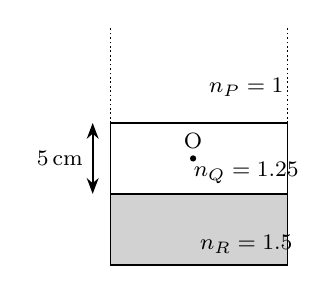
\begin{tikzpicture}[scale=0.75]
\fill[gray!35] (0,0) rectangle (3,1.2);
\draw (0,0) rectangle (3,2.4); \draw[densely dotted] (0,2.4) -- (0,4) (3,2.4) -- (3,4);
\draw (0,1.2) -- (3,1.2);
\node[lbl] at (2.3,3.0) {$n_P = 1$}; \node[lbl] at (2.3,1.55) {$n_Q = 1.25$}; \node[lbl] at (2.3,0.35) {$n_R = 1.5$};
\draw[<->] (-0.3,1.2) -- (-0.3,2.4) node[midway,left,lbl]{5\,cm};
\fill (1.4,1.8) circle (1.5pt) node[above,lbl]{O};
\end{tikzpicture}}\ntag{A}{229}{leph201}{9}{}{Class XII Part 2 \textperiodcentered{} Ch 9}}
{\opt{0}{1}{2}{3}}
\numoptstrue
\QQ{\qsrc{2023}{8}Light travels a distance $x$ in time $t_1$ in air and $10x$ in time $t_2$ in another denser medium. What is the critical angle for this medium?\ntag{A}{229}{leph201}{9}{}{Class XII Part 2 \textperiodcentered{} Ch 9}}
{\opt{$\sin^{-1}\!\left(\dfrac{10t_1}{t_2}\right)$}{$\sin^{-1}\!\left(\dfrac{t_2}{t_1}\right)$}{$\sin^{-1}\!\left(\dfrac{10t_2}{t_1}\right)$}{$\sin^{-1}\!\left(\dfrac{t_1}{10t_2}\right)$}}
\numoptstrue
\QQ{\qsrc{2022}{30}A light ray falls on a glass surface of refractive index $\sqrt3$, at an angle $60^\circ$. The angle between the refracted and reflected rays would be:\ntag{A}{228}{leph201}{8}{}{Class XII Part 2 \textperiodcentered{} Ch 9}}
{\opt{$120^\circ$}{$30^\circ$}{$60^\circ$}{$90^\circ$}}
\numoptstrue
\QQ{\qsrc{2022}{38}Two transparent media A and B are separated by a plane boundary. The speed of light in those media are $1.5\times10^8\unit{m/s}$ and $2.0\times10^8\unit{m/s}$, respectively. The critical angle for a ray of light for these two media is:\ntag{A}{229}{leph201}{9}{}{Class XII Part 2 \textperiodcentered{} Ch 9}}
{\opt{$\tan^{-1}(0.750)$}{$\sin^{-1}(0.500)$}{$\sin^{-1}(0.750)$}{$\tan^{-1}(0.500)$}}
\numoptstrue
\QQ{\qsrc{2019}{28}In total internal reflection when the angle of incidence is equal to the critical angle for the pair of media in contact, what will be angle of refraction?\ntag{D}{229}{leph201}{9}{ \textperiodcentered{} i = ic gives r = 90 deg}{Class XII Part 2 \textperiodcentered{} Ch 9}}
{\opt{$180^\circ$}{$0^\circ$}{equal to angle of incidence}{$90^\circ$}}
\topichead{Lenses and lens maker's formula}{8}
\numoptstrue
\QQ{\qsrc{2026}{29}The lens combination as shown in the figure, consists of two lenses, $L_1$ and $L_2$, of the focal lengths $+10\unit{cm}$ and $-10\unit{cm}$, respectively. The position of the image formed is:
\fig{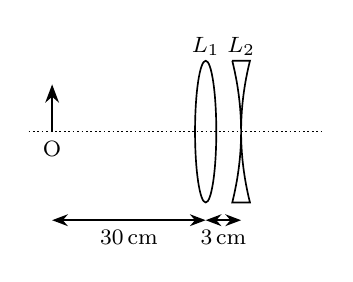
\begin{tikzpicture}[scale=0.75]
\draw[densely dotted] (-0.4,0) -- (4.6,0);
\draw[->,thick] (0,0) -- (0,0.8) node[left,lbl]{} ; \node[lbl,below] at (0,0) {O};
\draw (2.6,0) ellipse (0.18 and 1.2); \node[lbl] at (2.6,1.45) {$L_1$};
\draw (3.05,1.2) -- (3.35,1.2) .. controls (3.15,0.4) and (3.15,-0.4) .. (3.35,-1.2) -- (3.05,-1.2) .. controls (3.25,-0.4) and (3.25,0.4) .. (3.05,1.2); \node[lbl] at (3.2,1.45) {$L_2$};
\draw[<->] (0,-1.5) -- (2.6,-1.5) node[midway,below,lbl]{30\,cm}; \draw[<->] (2.6,-1.5) -- (3.2,-1.5) node[midway,below,lbl]{3\,cm};
\end{tikzpicture}}\ntag{A}{238}{leph201}{18}{}{Class XII Part 2 \textperiodcentered{} Ch 9}}
{\opt{20\,cm to the left of the concave lens}{60\,cm to the left of the concave lens}{30\,cm to the right of the concave lens}{60\,cm to the right of the concave lens}}
\numoptstrue
\QQ{\qsrc{2025}{13}In a certain camera, a combination of four similar thin convex lenses are arranged axially in contact. Then the power of the combination and the total magnification in comparison to the power ($p$) and magnification ($m$) for each lens will be, respectively\ntag{D}{238}{leph201}{18}{ \textperiodcentered{} P=sum Pi, m=m1 m2 m3}{Class XII Part 2 \textperiodcentered{} Ch 9}}
{\opt{$4p$ and $4m$}{$p^4$ and $4m$}{$4p$ and $m^4$}{$p^4$ and $m^4$}}
\numoptstrue
\QQ{\qsrc{2023}{45}In the figure shown here, what is the equivalent focal length of the combination of lenses (Assume that all layers are thin)?
\fig{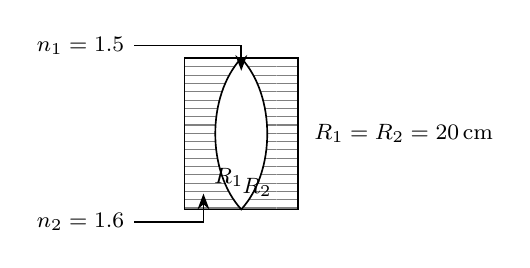
\begin{tikzpicture}[scale=0.8]
\fill[pattern=horizontal lines,pattern color=gray] (0,0) rectangle (1.8,2.4); \draw (0,0) rectangle (1.8,2.4);
\fill[white] (0.9,2.4) .. controls (0.35,1.8) and (0.35,0.6) .. (0.9,0) .. controls (1.45,0.6) and (1.45,1.8) .. (0.9,2.4);
\draw (0.9,2.4) .. controls (0.35,1.8) and (0.35,0.6) .. (0.9,0) .. controls (1.45,0.6) and (1.45,1.8) .. (0.9,2.4);
\node[lbl] at (0.7,0.5) {$R_1$}; \node[lbl] at (1.15,0.35) {$R_2$};
\draw[->] (-0.8,2.6) node[left,lbl]{$n_1 = 1.5$} -- (0.9,2.6) -- (0.9,2.2); \draw[->] (-0.8,-0.2) node[left,lbl]{$n_2 = 1.6$} -- (0.3,-0.2) -- (0.3,0.25);
\node[lbl,right] at (1.9,1.2) {$R_1 = R_2 = 20\unit{cm}$};
\end{tikzpicture}}\ntag{A}{238}{leph201}{18}{}{Class XII Part 2 \textperiodcentered{} Ch 9}}
{\opt{$-50\unit{cm}$}{40\,cm}{$-40\unit{cm}$}{$-100\unit{cm}$}}
\numoptstrue
\QQ{\qsrc{2023}{46}Two thin lenses are of same focal lengths ($f$), but one is convex and the other one is concave. When they are placed in contact with each other, the equivalent focal length of the combination will be:\ntag{D}{237}{leph201}{17}{ \textperiodcentered{} 1/f=1/f1+1/f2}{Class XII Part 2 \textperiodcentered{} Ch 9}}
{\opt{Infinite}{Zero}{$f/4$}{$f/2$}}
\numoptstrue
\QQ{\qsrc{2022}{8}A biconvex lens has radii of curvature, $20\unit{cm}$ each. If the refractive index of the material of the lens is 1.5, the power of the lens is:\ntag{D}{234}{leph201}{14}{ \textperiodcentered{} lens maker's formula}{Class XII Part 2 \textperiodcentered{} Ch 9}}
{\opt{infinity}{$+2$\,D}{$+20$\,D}{$+5$\,D}}
\numoptstrue
\QQ{\qsrc{2021}{8}A convex lens `A' of focal length $20\unit{cm}$ and a concave lens `B' of focal length $5\unit{cm}$ are kept along the same axis with a distance `$d$' between them. If a parallel beam of light falling on `A' leaves `B' as a parallel beam, then the distance `$d$' in cm will be:\ntag{A}{238}{leph201}{18}{}{Class XII Part 2 \textperiodcentered{} Ch 9}}
{\opt{25}{15}{50}{30}}
\numoptstrue
\QQ{\qsrc{2021}{41}A point object is placed at a distance of $60\unit{cm}$ from a convex lens of focal length $30\unit{cm}$. If a plane mirror were put perpendicular to the principal axis of the lens and at a distance of $40\unit{cm}$ from it, the final image would be formed at a distance of:\ntag{A}{238}{leph201}{18}{}{Class XII Part 2 \textperiodcentered{} Ch 9}}
{\opt{20\,cm from the lens, it would be a real image.}{30\,cm from the lens, it would be a real image.}{30\,cm from the plane mirror, it would be a virtual image.}{20\,cm from the plane mirror, it would be a virtual image.}}
\numoptstrue
\QQ{\qsrc{2019}{11}Two similar thin equi-convex lenses, of focal length $f$ each, are kept coaxially in contact with each other such that the focal length of the combination is $F_1$. When the space between the two lenses is filled with glycerin (which has the same refractive index ($\mu = 1.5$) as that of glass) then the equivalent focal length is $F_2$. The ratio $F_1:F_2$ will be:\ntag{A}{238}{leph201}{18}{}{Class XII Part 2 \textperiodcentered{} Ch 9}}
{\opt{2:1}{1:2}{2:3}{3:4}}
\topichead{Prism and dispersion}{6}
\numoptstrue
\QQ{\qsrc{2024}{6}A light ray enters through a right angled prism at point P with the angle of incidence $30^\circ$ as shown in figure. It travels through the prism parallel to its base BC and emerges along the face AC. The refractive index of the prism is:
\fig{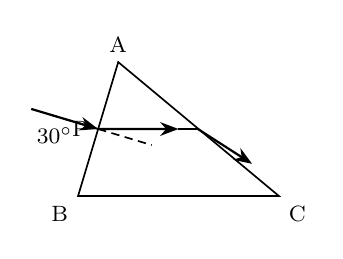
\begin{tikzpicture}[scale=0.85]
\coordinate (A) at (0.6,2.0); \coordinate (B) at (0,0); \coordinate (C) at (3.0,0);
\draw (A) -- (B) -- (C) -- cycle; \node[lbl,above] at (A) {A}; \node[lbl,below left] at (B) {B}; \node[lbl,below right] at (C) {C};
\coordinate (P) at (0.3,1.0); \node[lbl,left] at (P) {P};
\draw[thick,->] (-0.7,1.3) -- (P); \draw[thick,->] (P) -- (1.5,1.0); \draw[thick] (1.5,1.0) -- (1.79,1.0);
\draw[thick,->] (1.79,1.0) -- (2.6,0.48);
\draw[densely dashed] (P) -- +(-0.8,0.24) (P) -- +(0.8,-0.24); \node[lbl] at (-0.35,0.9) {$30^\circ$};
\end{tikzpicture}}\ntag{A}{240}{leph201}{20}{}{Class XII Part 2 \textperiodcentered{} Ch 9}}
{\opt{$\dfrac{\sqrt3}2$}{$\dfrac{\sqrt5}4$}{$\dfrac{\sqrt5}2$}{$\dfrac{\sqrt3}4$}}
\numoptstrue
\QQ{\qsrc{2021}{5}Find the value of the angle of emergence from the prism. Refractive index of the glass is $\sqrt3$.
\fig{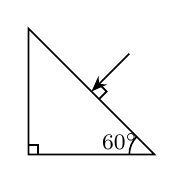
\begin{tikzpicture}[scale=0.8]
\draw (0,0) -- (2,0) -- (0,2) -- cycle; \draw (0,0) rectangle (0.15,0.15);
\draw (1.6,0) arc (180:135:0.4); \node[lbl] at (1.45,0.2) {$60^\circ$};
\draw[->] (1.6,1.6) -- (1.0,1.0); \draw (1.0,1.0) ++(0.12,0.12) -- ++(0.12,-0.12) -- ++(-0.12,-0.12);
\end{tikzpicture}}\ntag{A}{239}{leph201}{19}{}{Class XII Part 2 \textperiodcentered{} Ch 9}}
{\opt{$60^\circ$}{$30^\circ$}{$45^\circ$}{$90^\circ$}}
\numoptstrue
\QQ{\qsrc{2020}{140}A ray is incident at an angle of incidence $i$ on one surface of a small angle prism (with angle of prism $A$) and emerges normally from the opposite surface. If the refractive index of the material of the prism is $\mu$, then the angle of incidence is nearly equal to:\ntag{A}{239}{leph201}{19}{}{Class XII Part 2 \textperiodcentered{} Ch 9}}
{\opt{$\dfrac A{2\mu}$}{$\dfrac{2A}\mu$}{$\mu A$}{$\dfrac{\mu A}2$}}
\numoptstrue
\QQ{\qsrc{2018}{19}The refractive index of the material of a prism is $\sqrt2$ and the angle of the prism is $30^\circ$. One of the two refracting surfaces of the prism is made a mirror inwards, by silver coating. A beam of monochromatic light entering the prism from the other face will retrace its path (after reflection from the silvered surface) if its angle of incidence on the prism is\ntag{A}{240}{leph201}{20}{}{Class XII Part 2 \textperiodcentered{} Ch 9}}
{\opt{$30^\circ$}{$45^\circ$}{$60^\circ$}{zero}}
\numoptstrue
\QQ{\qsrc{2017}{152}A thin prism having refracting angle $10^\circ$ is made of glass of refractive index 1.42. This prism is combined with another thin prism of glass of refractive index 1.7. This combination produces dispersion without deviation. The refracting angle of second prism should be:\ntag{A}{238}{leph201}{18}{ \textperiodcentered{} thin prism delta=(mu-1)A}{Class XII Part 2 \textperiodcentered{} Ch 9}}
{\opt{$6^\circ$}{$8^\circ$}{$10^\circ$}{$4^\circ$}}
\numoptstrue
\QQ{\qsrc{2016}{22}The angle of incidence for a ray of light at a refracting surface of a prism is $45^\circ$. The angle of prism is $60^\circ$. If the ray suffers minimum deviation through the prism, the angle of minimum deviation and refractive index of the material of the prism respectively, are:\ntag{A}{240}{leph201}{20}{ \textperiodcentered{} minimum deviation}{Class XII Part 2 \textperiodcentered{} Ch 9}}
{\opt{$45^\circ$; $\dfrac1{\sqrt2}$}{$30^\circ$; $\sqrt2$}{$45^\circ$; $\sqrt2$}{$30^\circ$; $\dfrac1{\sqrt2}$}}
\topichead{Optical instruments (microscope, telescope)}{5}
\numoptstrue
\QQ{\qsrc{2025}{2}A microscope has an objective of focal length $2\unit{cm}$, eyepiece of focal length $4\unit{cm}$ and the tube length of $40\unit{cm}$. If the distance of distinct vision of eye is $25\unit{cm}$, the magnification in the microscope is\ntag{D}{244}{leph201}{24}{ \textperiodcentered{} m=(L/fo)(D/fe)}{Class XII Part 2 \textperiodcentered{} Ch 9}}
{\opt{100}{125}{150}{250}}
\numoptstrue
\QQ{\qsrc{2024}{36}A small telescope has an objective of focal length $140\unit{cm}$ and an eye piece of focal length $5.0\unit{cm}$. The magnifying power of telescope for viewing a distant object is:\ntag{D}{253}{leph201}{33}{ \textperiodcentered{} Exercise 9.27}{Class XII Part 2 \textperiodcentered{} Ch 9}}
{\opt{32}{34}{28}{17}}
\numoptstrue
\QQ{\qsrc{2021}{18}A lens of large focal length and large aperture is best suited as an objective of an astronomical telescope since:\ntag{D}{245}{leph201}{25}{ \textperiodcentered{} light gathering and resolution}{Class XII Part 2 \textperiodcentered{} Ch 9}}
{\opt{a large aperture contributes to the quality and visibility of the images.}{a large area of the objective ensures better light gathering power.}{a large aperture provides a better resolution.}{all of the above.}}
\numoptstrue
\QQ{\qsrc{2018}{10}An astronomical refracting telescope will have large angular magnification and high angular resolution, when it has an objective lens of\ntag{D}{245}{leph201}{25}{ \textperiodcentered{} light gathering and resolution}{Class XII Part 2 \textperiodcentered{} Ch 9}}
{\opt{large focal length and large diameter}{large focal length and small diameter}{small focal length and large diameter}{small focal length and small diameter}}
\numoptstrue
\QQ{\qsrc{2016}{32}A astronomical telescope has objective and eyepiece of focal lengths $40\unit{cm}$ and $4\unit{cm}$ respectively. To view an object $200\unit{cm}$ away from the objective, the lenses must be separated by a distance:\ntag{A}{243}{leph201}{23}{}{Class XII Part 2 \textperiodcentered{} Ch 9}}
{\opt{37.3\,cm}{46.0\,cm}{50.0\,cm}{54.0\,cm}}
\end{multicols}
\par\needspace{12\baselineskip}\vspace{12pt}
\begin{center}{\pgfornament[width=3.2cm,color=gilt]{87}}\par
{\large\color{navy}\scshape Ray Optics and Optical Instruments \textperiodcentered{} Answer Key}\end{center}
{\small\setlength{\tabcolsep}{1pt}\renewcommand{\arraystretch}{1.5}
\begin{tabularx}{\linewidth}{@{}*{8}{>{\centering\arraybackslash}X}@{}}\toprule
\textbf{1}\,(2) & \textbf{2}\,(4) & \textbf{3}\,(1) & \textbf{4}\,(2) & \textbf{5}\,(1) & \textbf{6}\,(4) & \textbf{7}\,(3) & \textbf{8}\,(4)\\
\textbf{9}\,(2) & \textbf{10}\,(3) & \textbf{11}\,(4) & \textbf{12}\,(1) & \textbf{13}\,(4) & \textbf{14}\,(2) & \textbf{15}\,(4) & \textbf{16}\,(2)\\
\textbf{17}\,(3) & \textbf{18}\,(1) & \textbf{19}\,(3) & \textbf{20}\,(2) & \textbf{21}\,(1) & \textbf{22}\,(2) & \textbf{23}\,(2) & \textbf{24}\,(3)\\
\textbf{25}\,(4) & \textbf{26}\,(1) & \textbf{27}\,(4) &  &  &  &  & \\\bottomrule\end{tabularx}}\par\smallskip
{\footnotesize Answers of 2021, 2022, 2023, 2025 and 2026 are from the official NTA final keys (checked by the editor); answers of 2016--2020 and 2024 were solved by the editor.
}\par
\par\needspace{18\baselineskip}\vspace{14pt}
\begin{center}{\pgfornament[width=3.2cm,color=gilt]{87}}\par
{\large\color{navy}\scshape Chapter Summary \textperiodcentered{} Ray Optics and Optical Instruments}\end{center}
{\small\setlength{\tabcolsep}{3.5pt}
\begin{tabular*}{\linewidth}{@{\extracolsep{\fill}}l*{11}{c}c@{}}\toprule
Year & 2016 & 2017 & 2018 & 2019 & 2020 & 2021 & 2022 & 2023 & 2024 & 2025 & 2026 & Total\\\midrule
Questions & 3 & 2 & 3 & 2 & 1 & 4 & 3 & 3 & 2 & 2 & 2 & \textbf{27}\\\bottomrule\end{tabular*}}\par\medskip
{\small\textbf{\color{crimson}Topic-wise} (in textbook order)\par\smallskip
\begin{tabularx}{\linewidth}{@{}>{\raggedright\arraybackslash}Xrrrl@{}}\toprule
Topic & Qs & Direct & Years & 2016 $\rightarrow$ 2026\\\midrule
Reflection and spherical mirrors & \textbf{3} & 0 & 3 & {\scriptsize \textbf{16} \textbf{17} \textbf{18} {\color{gray!45}19} {\color{gray!45}20} {\color{gray!45}21} {\color{gray!45}22} {\color{gray!45}23} {\color{gray!45}24} {\color{gray!45}25} {\color{gray!45}26}}\\
Refraction and total internal reflection & \textbf{5} & 1 & 4 & {\scriptsize {\color{gray!45}16} {\color{gray!45}17} {\color{gray!45}18} \textbf{19} {\color{gray!45}20} {\color{gray!45}21} \textbf{22} \textbf{23} {\color{gray!45}24} {\color{gray!45}25} \textbf{26}}\\
Lenses and lens maker's formula & \textbf{8} & 3 & 6 & {\scriptsize {\color{gray!45}16} {\color{gray!45}17} {\color{gray!45}18} \textbf{19} {\color{gray!45}20} \textbf{21} \textbf{22} \textbf{23} {\color{gray!45}24} \textbf{25} \textbf{26}}\\
Prism and dispersion & \textbf{6} & 0 & 6 & {\scriptsize \textbf{16} \textbf{17} \textbf{18} {\color{gray!45}19} \textbf{20} \textbf{21} {\color{gray!45}22} {\color{gray!45}23} \textbf{24} {\color{gray!45}25} {\color{gray!45}26}}\\
Optical instruments (microscope, telescope) & \textbf{5} & 4 & 5 & {\scriptsize \textbf{16} {\color{gray!45}17} \textbf{18} {\color{gray!45}19} {\color{gray!45}20} \textbf{21} {\color{gray!45}22} {\color{gray!45}23} \textbf{24} \textbf{25} {\color{gray!45}26}}\\
\bottomrule\end{tabularx}}\par\medskip
\begin{minipage}[t]{0.34\linewidth}{\small\textbf{\color{crimson}Direct vs Applied}\par\smallskip
\begin{tabular}{@{}lrr@{}}\toprule
Direct from NCERT & \textbf{8} & 30\%\\
\quad text, table, figure & 7 &\\
\quad solved Example & 0 &\\
\quad Exercise & 1 &\\
Applied & \textbf{19} & 70\%\\\midrule
Easy / Mod. / Hard & \multicolumn{2}{r}{9 / 16 / 2}\\\bottomrule
\end{tabular}}\end{minipage}\hfill
\begin{minipage}[t]{0.63\linewidth}{\small\textbf{\color{crimson}What to focus on}\par\smallskip
\begin{itemize}[leftmargin=1.1em,itemsep=1pt,topsep=0pt]
\item 27 questions in 11 papers, about 2.5 per paper; rank 2 of 28 chapters by number of questions.
\item Most asked topic: \textbf{Lenses and lens maker's formula} (8 questions, in 6 of the 11 years).
\item 1 questions are NCERT solved Examples or Exercises: Exercise 9.27 (Q 24). Work these by hand.
\item NCERT pages that gave three or more questions: page 238 (7 questions), page 229 (4 questions), page 240 (3 questions). Read these pages line by line.
\item Difficulty: 9 easy, 16 moderate, 2 hard (hard: Q 11, 15).
\item 19 applied questions: practise these after the NCERT Examples and Exercises of the chapter.
\end{itemize}}\end{minipage}\par
\chapterpaper{Class XII \textperiodcentered{} Chapter 10}{Wave Optics}{11 questions \textperiodcentered{} 2 topics \textperiodcentered{} NEET 2016--2026}{cleph202}{XII.10 Wave Optics}
\begin{multicols}{2}
\topichead{Young's double-slit interference}{9}
\numoptstrue
\QQ{\qsrc{2024}{35}If the monochromatic source in Young's double slit experiment is replaced by white light, then\ntag{A}{266}{leph202}{12}{}{Class XII Part 2 \textperiodcentered{} Ch 10}}
{\opt{all bright fringes will be of equal width.}{interference pattern will disappear.}{there will be a central dark fringe surrounded by a few coloured fringes.}{there will be a central bright white fringe surrounded by a few coloured fringes.}}
\numoptstrue
\QQ{\qsrc{2023}{24}For Young's double slit experiment, two statements are given below:\par
\textbf{Statement I}: If screen is moved away from the plane of slits, angular separation of the fringes remains constant.\par
\textbf{Statement II}: If the monochromatic source is replaced by another monochromatic source of larger wavelength, the angular separation of fringes decreases.\par
In the light of the above statements, choose the \textit{correct} answer from the options given below:\ntag{A}{266}{leph202}{12}{}{Class XII Part 2 \textperiodcentered{} Ch 10}}
{\opt{Statement I is false but Statement II is true.}{Both Statement I and Statement II are true.}{Both Statement I and Statement II are false.}{Statement I is true but Statement II is false.}}
\numoptstrue
\QQ{\qsrc{2022}{29}In a Young's double slit experiment, a student observes 8 fringes in a certain segment of screen when a monochromatic light of $600\unit{nm}$ wavelength is used. If the wavelength of light is changed to $400\unit{nm}$, then the number of fringes he would observe in the same region of the screen is:\ntag{A}{266}{leph202}{12}{}{Class XII Part 2 \textperiodcentered{} Ch 10}}
{\opt{12}{6}{8}{9}}
\numoptstrue
\QQ{\qsrc{2020}{165}In Young's double slit experiment, if the separation between coherent sources is halved and the distance of the screen from the coherent sources is doubled, then the fringe width becomes:\ntag{A}{266}{leph202}{12}{}{Class XII Part 2 \textperiodcentered{} Ch 10}}
{\opt{double}{half}{four times}{one-fourth}}
\numoptstrue
\QQ{\qsrc{2019}{5}In a double slit experiment, when light of wavelength $400\unit{nm}$ was used, the angular width of the first minima formed on a screen placed $1\unit{m}$ away, was found to be $0.2^\circ$. What will be the angular width of the first minima, if the entire experimental apparatus is immersed in water? ($\mu_{\text{water}} = 4/3$)\ntag{A}{267}{leph202}{13}{}{Class XII Part 2 \textperiodcentered{} Ch 10}}
{\opt{$0.266^\circ$}{$0.15^\circ$}{$0.05^\circ$}{$0.1^\circ$}}
\numoptstrue
\QQ{\qsrc{2018}{9}In Young's double slit experiment the separation $d$ between the slits is $2\unit{mm}$, the wavelength $\lambda$ of the light used is $5896\unit{\text{\AA}}$ and distance $D$ between the screen and slits is $100\unit{cm}$. It is found that the angular width of the fringes is $0.20^\circ$. To increase the fringe angular width to $0.21^\circ$ (with same $\lambda$ and $D$) the separation between the slits needs to be changed to\ntag{A}{266}{leph202}{12}{}{Class XII Part 2 \textperiodcentered{} Ch 10}}
{\opt{2.1\,mm}{1.9\,mm}{1.8\,mm}{1.7\,mm}}
\numoptstrue
\QQ{\qsrc{2017}{137}Young's double slit experiment is first performed in air and then in a medium other than air. It is found that $8^{\text{th}}$ bright fringe in the medium lies where $5^{\text{th}}$ dark fringe lies in air. The refractive index of the medium is nearly:\ntag{A}{266}{leph202}{12}{}{Class XII Part 2 \textperiodcentered{} Ch 10}}
{\opt{1.59}{1.69}{1.78}{1.25}}
\numoptstrue
\QQ{\qsrc{2016}{6}In a diffraction pattern due to a single slit of width `$a$', the first minimum is observed at an angle $30^\circ$ when light of wavelength $5000\unit{\text{\AA}}$ is incident on the slit. The first secondary maximum is observed at an angle of:\ntag{A}{267}{leph202}{13}{ \textperiodcentered{} single slit}{Class XII Part 2 \textperiodcentered{} Ch 10}}
{\opt{$\sin^{-1}\!\left(\dfrac14\right)$}{$\sin^{-1}\!\left(\dfrac23\right)$}{$\sin^{-1}\!\left(\dfrac12\right)$}{$\sin^{-1}\!\left(\dfrac34\right)$}}
\numoptstrue
\QQ{\qsrc{2016}{18}The intensity at the maximum in a Young's double slit experiment is $I_0$. Distance between two slits is $d = 5\lambda$, where $\lambda$ is the wavelength of light used in the experiment. What will be the intensity in front of one of the slits on the screen placed at a distance $D = 10d$?\ntag{A}{266}{leph202}{12}{}{Class XII Part 2 \textperiodcentered{} Ch 10}}
{\opt{$I_0$}{$\dfrac{I_0}4$}{$\dfrac34I_0$}{$\dfrac{I_0}2$}}
\topichead{Polarisation and Malus' law}{2}
\numoptstrue
\QQ{\qsrc{2025}{43}The intensity of transmitted light when a polaroid sheet, placed between two crossed polaroids at $22.5^\circ$ from the polarization axis of one of the polaroid, is ($I_0$ is the intensity of polarised light after passing through the first polaroid):\ntag{D}{271}{leph202}{17}{ \textperiodcentered{} Example 10.2}{Class XII Part 2 \textperiodcentered{} Ch 10}}
{\opt{$\dfrac{I_0}2$}{$\dfrac{I_0}4$}{$\dfrac{I_0}8$}{$\dfrac{I_0}{16}$}}
\numoptstrue
\QQ{\qsrc{2017}{174}Two Polaroids $P_1$ and $P_2$ are placed with their axis perpendicular to each other. Unpolarised light $I_0$ is incident on $P_1$. A third polaroid $P_3$ is kept in between $P_1$ and $P_2$ such that its axis makes an angle $45^\circ$ with that of $P_1$. The intensity of transmitted light through $P_2$ is:\ntag{A}{271}{leph202}{17}{}{Class XII Part 2 \textperiodcentered{} Ch 10}}
{\opt{$\dfrac{I_0}4$}{$\dfrac{I_0}8$}{$\dfrac{I_0}{16}$}{$\dfrac{I_0}2$}}
\end{multicols}
\par\needspace{12\baselineskip}\vspace{12pt}
\begin{center}{\pgfornament[width=3.2cm,color=gilt]{87}}\par
{\large\color{navy}\scshape Wave Optics \textperiodcentered{} Answer Key}\end{center}
{\small\setlength{\tabcolsep}{1pt}\renewcommand{\arraystretch}{1.5}
\begin{tabularx}{\linewidth}{@{}*{8}{>{\centering\arraybackslash}X}@{}}\toprule
\textbf{1}\,(4) & \textbf{2}\,(4) & \textbf{3}\,(1) & \textbf{4}\,(3) & \textbf{5}\,(2) & \textbf{6}\,(2) & \textbf{7}\,(3) & \textbf{8}\,(4)\\
\textbf{9}\,(4) & \textbf{10}\,(3) & \textbf{11}\,(2) &  &  &  &  & \\\bottomrule\end{tabularx}}\par\smallskip
{\footnotesize Answers of 2021, 2022, 2023, 2025 and 2026 are from the official NTA final keys (checked by the editor); answers of 2016--2020 and 2024 were solved by the editor.
}\par
\par\needspace{18\baselineskip}\vspace{14pt}
\begin{center}{\pgfornament[width=3.2cm,color=gilt]{87}}\par
{\large\color{navy}\scshape Chapter Summary \textperiodcentered{} Wave Optics}\end{center}
{\small\setlength{\tabcolsep}{3.5pt}
\begin{tabular*}{\linewidth}{@{\extracolsep{\fill}}l*{11}{c}c@{}}\toprule
Year & 2016 & 2017 & 2018 & 2019 & 2020 & 2021 & 2022 & 2023 & 2024 & 2025 & 2026 & Total\\\midrule
Questions & 2 & 2 & 1 & 1 & 1 & 0 & 1 & 1 & 1 & 1 & 0 & \textbf{11}\\\bottomrule\end{tabular*}}\par\medskip
{\small\textbf{\color{crimson}Topic-wise} (in textbook order)\par\smallskip
\begin{tabularx}{\linewidth}{@{}>{\raggedright\arraybackslash}Xrrrl@{}}\toprule
Topic & Qs & Direct & Years & 2016 $\rightarrow$ 2026\\\midrule
Young's double-slit interference & \textbf{9} & 0 & 8 & {\scriptsize \textbf{16} \textbf{17} \textbf{18} \textbf{19} \textbf{20} {\color{gray!45}21} \textbf{22} \textbf{23} \textbf{24} {\color{gray!45}25} {\color{gray!45}26}}\\
Polarisation and Malus' law & \textbf{2} & 1 & 2 & {\scriptsize {\color{gray!45}16} \textbf{17} {\color{gray!45}18} {\color{gray!45}19} {\color{gray!45}20} {\color{gray!45}21} {\color{gray!45}22} {\color{gray!45}23} {\color{gray!45}24} \textbf{25} {\color{gray!45}26}}\\
\bottomrule\end{tabularx}}\par\medskip
\begin{minipage}[t]{0.34\linewidth}{\small\textbf{\color{crimson}Direct vs Applied}\par\smallskip
\begin{tabular}{@{}lrr@{}}\toprule
Direct from NCERT & \textbf{1} & 9\%\\
\quad text, table, figure & 0 &\\
\quad solved Example & 1 &\\
\quad Exercise & 0 &\\
Applied & \textbf{10} & 91\%\\\midrule
Easy / Mod. / Hard & \multicolumn{2}{r}{3 / 7 / 1}\\\bottomrule
\end{tabular}}\end{minipage}\hfill
\begin{minipage}[t]{0.63\linewidth}{\small\textbf{\color{crimson}What to focus on}\par\smallskip
\begin{itemize}[leftmargin=1.1em,itemsep=1pt,topsep=0pt]
\item 11 questions in 11 papers, about 1.0 per paper; rank 24 of 28 chapters by number of questions.
\item Most asked topic: \textbf{Young's double-slit interference} (9 questions, in 8 of the 11 years).
\item Asked in 8 or more of the 11 years: Young's double-slit interference.
\item 1 questions are NCERT solved Examples or Exercises: Example 10.2 (Q 10). Work these by hand.
\item NCERT pages that gave three or more questions: page 266 (7 questions). Read these pages line by line.
\item Difficulty: 3 easy, 7 moderate, 1 hard (hard: Q 9).
\item 10 applied questions: practise these after the NCERT Examples and Exercises of the chapter.
\end{itemize}}\end{minipage}\par
\chapterpaper{Class XII \textperiodcentered{} Chapter 11}{Dual Nature of Radiation and Matter}{22 questions \textperiodcentered{} 3 topics \textperiodcentered{} NEET 2016--2026}{cleph203}{XII.11 Dual Nature of Radiation and Matter}
\begin{multicols}{2}
\topichead{Photoelectric effect}{9}
\numoptstrue
\QQ{\qsrc{2026}{8}A beam of light falls on a metal surface such that photo-electrons are generated. If power of the light source starts to decrease linearly with time $t$, then variation of the photocurrent $I$ and magnitude of the stopping potential $|V|$ with time is best represented by:\ntag{D}{278}{leph203}{5}{ \textperiodcentered{} Figs 11.2, 11.3}{Class XII Part 2 \textperiodcentered{} Ch 11}}
{\optfig{\gaxes{$t$}{$I$}{\draw (0,1.5) -- (1.6,0.1);}\,\gaxes{$t$}{$|V|$}{\draw (0,1.2) -- (1.8,1.2);}}
{\gaxes{$t$}{$I$}{\draw (0,1.5) -- (1.6,0.1);}\,\gaxes{$t$}{$|V|$}{\draw (0,1.5) -- (1.6,0.1);}}
{\gaxes{$t$}{$I$}{\draw (0,1.2) -- (1.8,1.2);}\,\gaxes{$t$}{$|V|$}{\draw (0,1.5) -- (1.6,0.1);}}
{\gaxes{$t$}{$I$}{\draw (0,1.2) -- (1.8,1.2);}\,\gaxes{$t$}{$|V|$}{\draw (0,1.2) -- (1.8,1.2);}}}
\numoptstrue
\QQ{\qsrc{2026}{18}A ray of light with wavelength $\lambda$ is incident on three different photoelectric cells namely 1, 2 and 3. The threshold wavelength of these photoelectric cells are $\lambda_1$, $\lambda_2$, and $\lambda_3$, respectively and the magnitude of stopping potentials of these cells are $V_1$, $V_2$ and $V_3$, respectively. The relation between $\lambda$ and threshold wavelengths are $\lambda_1<\lambda$, $\lambda_2>\lambda$ and $\lambda_3\gg\lambda$. The correct option is:\ntag{A}{281}{leph203}{8}{}{Class XII Part 2 \textperiodcentered{} Ch 11}}
{\opt{$V_1 = 0$, $V_2<V_3$}{$V_1 = 0$, $V_2>V_3$}{$V_1>V_2$, $V_3 = 0$}{$V_1<V_2$, $V_3 = 0$}}
\numoptstrue
\QQ{\qsrc{2025}{38}Which of the following options represent the variation of photoelectric current with property of light shown on the $x$-axis?
\fig{\begin{tabular}{@{}cc@{}}
A.\ \gaxes{\tiny Intensity}{\tiny Current}{\draw (0,0) -- (1.6,1.5);} & B.\ \gaxes{\tiny Intensity}{\tiny Current}{\draw (0,1.2) -- (1.8,1.2);}\\
C.\ \gaxes{\tiny Frequency}{\tiny Current}{\draw (0,0) -- (1.6,1.5);} & D.\ \gaxes{\tiny Frequency}{\tiny Current}{\draw (0.5,0) -- (1.8,1.4);}
\end{tabular}}\ntag{D}{278}{leph203}{5}{ \textperiodcentered{} Figs 11.2 and 11.4}{Class XII Part 2 \textperiodcentered{} Ch 11}}
{\opt{A only}{A and C}{A and D}{B and D}}
\numoptstrue
\QQ{\qsrc{2023}{1}The work functions of Caesium (Cs), Potassium (K) and Sodium (Na) are $2.14\unit{eV}$, $2.30\unit{eV}$ and $2.75\unit{eV}$ respectively. If incident electromagnetic radiation has an incident energy of $2.20\unit{eV}$, which of these photosensitive surfaces may emit photoelectrons?\ntag{D}{281}{leph203}{8}{ \textperiodcentered{} Kmax=h nu - phi0}{Class XII Part 2 \textperiodcentered{} Ch 11}}
{\opt{Na only}{Cs only}{Both Na and K}{K only}}
\numoptstrue
\QQ{\qsrc{2022}{3}When two monochromatic lights of frequency, $\nu$ and $\dfrac\nu2$ are incident on a photoelectric metal, their stopping potential becomes $\dfrac{V_s}2$ and $V_s$ respectively. The threshold frequency for this metal is:\ntag{A}{281}{leph203}{8}{}{Class XII Part 2 \textperiodcentered{} Ch 11}}
{\opt{$\dfrac32\nu$}{$2\nu$}{$3\nu$}{$\dfrac23\nu$}}
\numoptstrue
\QQ{\qsrc{2020}{157}Light of frequency 1.5 times the threshold frequency is incident on a photosensitive material. What will be the photoelectric current if the frequency is halved and intensity is doubled?\ntag{A}{277}{leph203}{4}{}{Class XII Part 2 \textperiodcentered{} Ch 11}}
{\opt{doubled}{four times}{one-fourth}{zero}}
\numoptstrue
\QQ{\qsrc{2018}{14}When the light of frequency $2\nu_0$ (where $\nu_0$ is threshold frequency), is incident on a metal plate, the maximum velocity of electrons emitted is $v_1$. When the frequency of the incident radiation is increased to $5\nu_0$, the maximum velocity of electrons emitted from the same plate is $v_2$. The ratio of $v_1$ to $v_2$ is\ntag{A}{281}{leph203}{8}{}{Class XII Part 2 \textperiodcentered{} Ch 11}}
{\opt{4:1}{1:4}{1:2}{2:1}}
\numoptstrue
\QQ{\qsrc{2017}{158}The photoelectric threshold wavelength of silver is $3250\times10^{-10}\unit{m}$. The velocity of the electron ejected from a silver surface by ultraviolet light of wavelength $2536\times10^{-10}\unit{m}$ is: (Given $h = 4.14\times10^{-15}\unit{eV\,s}$ and $c = 3\times10^8\unit{m\,s^{-1}}$)\ntag{A}{278}{leph203}{5}{}{Class XII Part 2 \textperiodcentered{} Ch 11}}
{\opt{$\approx0.6\times10^6\unit{m\,s^{-1}}$}{$\approx61\times10^3\unit{m\,s^{-1}}$}{$\approx0.3\times10^6\unit{m\,s^{-1}}$}{$\approx6\times10^5\unit{m\,s^{-1}}$}}
\numoptstrue
\QQ{\qsrc{2016}{29}When a metallic surface is illuminated with radiation of wavelength $\lambda$, the stopping potential is $V$. If the same surface is illuminated with radiation of wavelength $2\lambda$, the stopping potential is $\dfrac V4$. The threshold wavelength for the metallic surface is:\ntag{A}{278}{leph203}{5}{}{Class XII Part 2 \textperiodcentered{} Ch 11}}
{\opt{$4\lambda$}{$5\lambda$}{$\dfrac52\lambda$}{$3\lambda$}}
\topichead{Photons and photon momentum}{4}
\numoptstrue
\QQ{\qsrc{2026}{19}A photon and an electron, each of $20\unit{eV}$ energy, move in free space. The ratio of linear momentum of electron $p_e$ to that of photon $p_{Ph}$, $\dfrac{p_e}{p_{Ph}}$ is: [Take speed of light $= 3\times10^8\unit{m\,s^{-1}}$, charge of electron $= -1.6\times10^{-19}\unit{C}$ and mass of electron $= 9\times10^{-31}\unit{kg}$]\ntag{A}{283}{leph203}{10}{}{Class XII Part 2 \textperiodcentered{} Ch 11}}
{\opt{$\dfrac2{450}$}{$\dfrac1{250}$}{225}{275}}
\numoptstrue
\QQ{\qsrc{2024}{24}If $c$ is the velocity of light in free space, the correct statements about photon among the following are:
\begin{stmts}[\Alph*.]
\item The energy of a photon is $E = h\nu$.
\item The velocity of a photon is $c$.
\item The momentum of a photon, $p = \dfrac{h\nu}c$.
\item In a photon-electron collision, both total energy and total momentum are conserved.
\item Photon possesses positive charge.
\end{stmts}
Choose the correct answer from the options given below:\ntag{D}{283}{leph203}{10}{ \textperiodcentered{} photon properties}{Class XII Part 2 \textperiodcentered{} Ch 11}}
{\opt{A, B, D and E only}{A and B only}{A, B, C and D only}{A, C and D only}}
\numoptstrue
\QQ{\qsrc{2023}{22}The minimum wavelength of X-rays produced by an electron accelerated through a potential difference of $V$ volts is proportional to:\ntag{D}{288}{leph203}{15}{ \textperiodcentered{} Exercise 11.1}{Class XII Part 2 \textperiodcentered{} Ch 11}}
{\opt{$V^2$}{$\sqrt V$}{$\dfrac1V$}{$\dfrac1{\sqrt V}$}}
\numoptstrue
\QQ{\qsrc{2021}{31}The number of photons per second on an average emitted by the source of monochromatic light of wavelength $600\unit{nm}$, when it delivers the power of $3.3\times10^{-3}$ watt will be: ($h = 6.6\times10^{-34}\unit{J\,s}$)\ntag{D}{284}{leph203}{11}{ \textperiodcentered{} Example 11.1}{Class XII Part 2 \textperiodcentered{} Ch 11}}
{\opt{$10^{18}$}{$10^{17}$}{$10^{16}$}{$10^{15}$}}
\topichead{de Broglie waves}{9}
\numoptstrue
\QQ{\qsrc{2025}{37}A photon and an electron (mass $m$) have the same energy $E$. The ratio ($\lambda_{\text{photon}}/\lambda_{\text{electron}}$) of their de Broglie wavelengths is: ($c$ is the speed of light)\ntag{A}{285}{leph203}{12}{}{Class XII Part 2 \textperiodcentered{} Ch 11}}
{\opt{$\sqrt{\dfrac E{2m}}$}{$c\sqrt{2mE}$}{$c\sqrt{\dfrac{2m}E}$}{$\dfrac1c\sqrt{\dfrac E{2m}}$}}
\numoptstrue
\QQ{\qsrc{2024}{8}The graph which shows the variation of $\left(\dfrac1{\lambda^2}\right)$ and its kinetic energy, $E$ is (where $\lambda$ is de Broglie wavelength of a free particle):\ntag{A}{285}{leph203}{12}{}{Class XII Part 2 \textperiodcentered{} Ch 11}}
{\optfig{\gaxes{$E$}{$\frac1{\lambda^2}$}{\draw (0,0) -- (1.6,1.5);}}
{\gaxes{$E$}{$\frac1{\lambda^2}$}{\draw (0,0) .. controls (1.0,0.1) and (1.4,0.6) .. (1.7,1.6);}}
{\gaxes{$E$}{$\frac1{\lambda^2}$}{\draw (0.1,1.6) .. controls (0.4,0.5) and (0.9,0.2) .. (1.8,0.1);}}
{\gaxes{$E$}{$\frac1{\lambda^2}$}{\draw (0,0) .. controls (0.2,1.0) and (0.7,1.5) .. (1.7,1.6);}}}
\numoptstrue
\QQ{\qsrc{2022}{9}The graph which shows the variation of the de Broglie wavelength ($\lambda$) of a particle and its associated momentum ($p$) is:\ntag{D}{285}{leph203}{12}{ \textperiodcentered{} lambda=h/p}{Class XII Part 2 \textperiodcentered{} Ch 11}}
{\optfig{\gaxes{$p$}{$\lambda$}{\draw (0.1,1.7) .. controls (0.3,0.4) and (0.7,0.2) .. (1.9,0.15);}}
{\gaxes{$p$}{$\lambda$}{\draw (0.2,0.2) -- (1.6,1.6);}}
{\gaxes{$p$}{$\lambda$}{\draw (0.1,1.6) -- (1.7,0.15);}}
{\gaxes{$p$}{$\lambda$}{\draw (0.1,0.15) .. controls (1.2,0.2) and (1.6,0.6) .. (1.7,1.7);}}}
\numoptstrue
\QQ{\qsrc{2021}{29}An electromagnetic wave of wavelength `$\lambda$' is incident on a photosensitive surface of negligible work function. If `$m$' mass is of photoelectron emitted from the surface has de-Broglie wavelength $\lambda_d$, then:\ntag{A}{285}{leph203}{12}{}{Class XII Part 2 \textperiodcentered{} Ch 11}}
{\opt{$\lambda = \left(\dfrac{2m}{hc}\right)\lambda_d^2$}{$\lambda_d = \left(\dfrac{2mc}h\right)\lambda^2$}{$\lambda = \left(\dfrac{2mc}h\right)\lambda_d^2$}{$\lambda = \left(\dfrac{2h}{mc}\right)\lambda_d^2$}}
\numoptstrue
\QQ{\qsrc{2020}{175}An electron is accelerated from rest through a potential difference of $V$ volt. If the de Broglie wavelength of the electron is $1.227\times10^{-2}\unit{nm}$, the potential difference is:\ntag{A}{286}{leph203}{13}{}{Class XII Part 2 \textperiodcentered{} Ch 11}}
{\opt{10\,V}{$10^2$\,V}{$10^3$\,V}{$10^4$\,V}}
\numoptstrue
\QQ{\qsrc{2019}{13}An electron is accelerated through a potential difference of $10{,}000\unit{V}$. Its de Broglie wavelength is, (nearly): ($m_e = 9\times10^{-31}\unit{kg}$)\ntag{A}{286}{leph203}{13}{}{Class XII Part 2 \textperiodcentered{} Ch 11}}
{\opt{$12.2\times10^{-13}\unit{m}$}{$12.2\times10^{-12}\unit{m}$}{$12.2\times10^{-14}\unit{m}$}{12.2\,nm}}
\numoptstrue
\QQ{\qsrc{2018}{12}An electron of mass $m$ with an initial velocity $\vec V = V_0\hat i$ ($V_0>0$) enters an electric field $\vec E = -E_0\hat i$ ($E_0$ = constant $>0$) at $t = 0$. If $\lambda_0$ is its de-Broglie wavelength initially, then its de-Broglie wavelength at time $t$ is\ntag{A}{285}{leph203}{12}{}{Class XII Part 2 \textperiodcentered{} Ch 11}}
{\opt{$\lambda_0t$}{$\lambda_0\left(1+\dfrac{eE_0}{mV_0}t\right)$}{$\dfrac{\lambda_0}{\left(1+\dfrac{eE_0}{mV_0}t\right)}$}{$\lambda_0$}}
\numoptstrue
\QQ{\qsrc{2017}{140}The de-Broglie wavelength of a neutron in thermal equilibrium with heavy water at a temperature $T$ (Kelvin) and mass $m$, is:\ntag{A}{285}{leph203}{12}{ \textperiodcentered{} thermal KE 3kT/2}{Class XII Part 2 \textperiodcentered{} Ch 11}}
{\opt{$\dfrac h{\sqrt{3mkT}}$}{$\dfrac{2h}{\sqrt{3mkT}}$}{$\dfrac{2h}{\sqrt{mkT}}$}{$\dfrac h{\sqrt{mkT}}$}}
\numoptstrue
\QQ{\qsrc{2016}{20}An electron of mass $m$ and a photon have same energy $E$. The ratio of de-Broglie wavelengths associated with them is: ($c$ being velocity of light)\ntag{A}{285}{leph203}{12}{}{Class XII Part 2 \textperiodcentered{} Ch 11}}
{\opt{$\dfrac1c\left(\dfrac E{2m}\right)^{1/2}$}{$\left(\dfrac E{2m}\right)^{1/2}$}{$c(2mE)^{1/2}$}{$\dfrac1c\left(\dfrac{2m}E\right)^{1/2}$}}
\end{multicols}
\par\needspace{12\baselineskip}\vspace{12pt}
\begin{center}{\pgfornament[width=3.2cm,color=gilt]{87}}\par
{\large\color{navy}\scshape Dual Nature of Radiation and Matter \textperiodcentered{} Answer Key}\end{center}
{\small\setlength{\tabcolsep}{1pt}\renewcommand{\arraystretch}{1.5}
\begin{tabularx}{\linewidth}{@{}*{8}{>{\centering\arraybackslash}X}@{}}\toprule
\textbf{1}\,(1) & \textbf{2}\,(1) & \textbf{3}\,(1) & \textbf{4}\,(2) & \textbf{5}\,(1) & \textbf{6}\,(4) & \textbf{7}\,(3) & \textbf{8}\,(1)$^{*}$\\
\textbf{9}\,(4) & \textbf{10}\,(3) & \textbf{11}\,(3) & \textbf{12}\,(3) & \textbf{13}\,(3) & \textbf{14}\,(3) & \textbf{15}\,(1) & \textbf{16}\,(1)\\
\textbf{17}\,(3) & \textbf{18}\,(4) & \textbf{19}\,(2) & \textbf{20}\,(3) & \textbf{21}\,(1) & \textbf{22}\,(1) &  & \\\bottomrule\end{tabularx}}\par\smallskip
{\footnotesize Answers of 2021, 2022, 2023, 2025 and 2026 are from the official NTA final keys (checked by the editor); answers of 2016--2020 and 2024 were solved by the editor. $^{*}$: see note.
\par\smallskip\textbf{8.} (NEET 2017 Q158) $K_{\max}\approx1.08$\,eV gives $v\approx6.2\times10^5$\,m/s; options (1) and (4) are the same value.
}\par
\par\needspace{18\baselineskip}\vspace{14pt}
\begin{center}{\pgfornament[width=3.2cm,color=gilt]{87}}\par
{\large\color{navy}\scshape Chapter Summary \textperiodcentered{} Dual Nature of Radiation and Matter}\end{center}
{\small\setlength{\tabcolsep}{3.5pt}
\begin{tabular*}{\linewidth}{@{\extracolsep{\fill}}l*{11}{c}c@{}}\toprule
Year & 2016 & 2017 & 2018 & 2019 & 2020 & 2021 & 2022 & 2023 & 2024 & 2025 & 2026 & Total\\\midrule
Questions & 2 & 2 & 2 & 1 & 2 & 2 & 2 & 2 & 2 & 2 & 3 & \textbf{22}\\\bottomrule\end{tabular*}}\par\medskip
{\small\textbf{\color{crimson}Topic-wise} (in textbook order)\par\smallskip
\begin{tabularx}{\linewidth}{@{}>{\raggedright\arraybackslash}Xrrrl@{}}\toprule
Topic & Qs & Direct & Years & 2016 $\rightarrow$ 2026\\\midrule
Photoelectric effect & \textbf{9} & 3 & 8 & {\scriptsize \textbf{16} \textbf{17} \textbf{18} {\color{gray!45}19} \textbf{20} {\color{gray!45}21} \textbf{22} \textbf{23} {\color{gray!45}24} \textbf{25} \textbf{26}}\\
Photons and photon momentum & \textbf{4} & 3 & 4 & {\scriptsize {\color{gray!45}16} {\color{gray!45}17} {\color{gray!45}18} {\color{gray!45}19} {\color{gray!45}20} \textbf{21} {\color{gray!45}22} \textbf{23} \textbf{24} {\color{gray!45}25} \textbf{26}}\\
de Broglie waves & \textbf{9} & 1 & 9 & {\scriptsize \textbf{16} \textbf{17} \textbf{18} \textbf{19} \textbf{20} \textbf{21} \textbf{22} {\color{gray!45}23} \textbf{24} \textbf{25} {\color{gray!45}26}}\\
\bottomrule\end{tabularx}}\par\medskip
\begin{minipage}[t]{0.34\linewidth}{\small\textbf{\color{crimson}Direct vs Applied}\par\smallskip
\begin{tabular}{@{}lrr@{}}\toprule
Direct from NCERT & \textbf{7} & 32\%\\
\quad text, table, figure & 5 &\\
\quad solved Example & 1 &\\
\quad Exercise & 1 &\\
Applied & \textbf{15} & 68\%\\\midrule
Easy / Mod. / Hard & \multicolumn{2}{r}{8 / 14 / 0}\\\bottomrule
\end{tabular}}\end{minipage}\hfill
\begin{minipage}[t]{0.63\linewidth}{\small\textbf{\color{crimson}What to focus on}\par\smallskip
\begin{itemize}[leftmargin=1.1em,itemsep=1pt,topsep=0pt]
\item 22 questions in 11 papers, about 2.0 per paper; rank 4 of 28 chapters by number of questions.
\item Most asked topic: \textbf{de Broglie waves} (9 questions, in 9 of the 11 years).
\item Asked in 8 or more of the 11 years: Photoelectric effect, de Broglie waves.
\item 2 questions are NCERT solved Examples or Exercises: Example 11.1 (Q 13), Exercise 11.1 (Q 12). Work these by hand.
\item NCERT pages that gave three or more questions: page 285 (7 questions), page 278 (4 questions), page 281 (4 questions). Read these pages line by line.
\item Difficulty: 8 easy, 14 moderate, 0 hard.
\item 15 applied questions: practise these after the NCERT Examples and Exercises of the chapter.
\end{itemize}}\end{minipage}\par
\chapterpaper{Class XII \textperiodcentered{} Chapter 12}{Atoms}{15 questions \textperiodcentered{} 2 topics \textperiodcentered{} NEET 2016--2026}{cleph204}{XII.12 Atoms}
\begin{multicols}{2}
\topichead{Alpha-particle scattering and atomic models}{3}
\numoptstrue
\QQ{\qsrc{2026}{35}In Geiger--Marsden experiment, the number of scattered $\alpha$-particles $N(\theta)$ is plotted as a function of scattering angle $\theta$. Which of the following options represents the correct plot? ($N(\theta)$ on a logarithmic scale, $\theta$ from $0^\circ$ to $180^\circ$.)\ntag{D}{293}{leph204}{4}{ \textperiodcentered{} Fig 12.3}{Class XII Part 2 \textperiodcentered{} Ch 12}}
{\optfig{\gaxes{$\theta$}{$N(\theta)$}{\draw (0.15,0.3) -- (1.8,1.5);}}
{\gaxes{$\theta$}{$N(\theta)$}{\draw (0.05,1.5) .. controls (0.8,1.55) and (1.4,1.0) .. (1.8,0.3);}}
{\gaxes{$\theta$}{$N(\theta)$}{\draw (0.05,1.6) .. controls (0.3,0.6) and (0.8,0.3) .. (1.8,0.2);}}
{\gaxes{$\theta$}{$N(\theta)$}{\draw (0.1,0.1) .. controls (0.5,0.2) and (0.5,1.5) .. (0.95,1.5) .. controls (1.4,1.5) and (1.4,0.2) .. (1.8,0.1);}}}
\numoptstrue
\QQ{\qsrc{2024}{22}Given below are two statements:\par
\textbf{Statement I}: Atoms are electrically neutral as they contain equal number of positive and negative charges.\par
\textbf{Statement II}: Atoms of each element are stable and emit their characteristic spectrum.\par
In the light of the above statements, choose the \textit{most appropriate} answer from the options given below:\ntag{D}{290}{leph204}{1}{}{Class XII Part 2 \textperiodcentered{} Ch 12}}
{\opt{Statement I is incorrect but Statement II is correct.}{Both Statement I and Statement II are correct.}{Both Statement I and Statement II are incorrect.}{Statement I is correct but Statement II is incorrect.}}
\numoptstrue
\QQ{\qsrc{2016}{23}When an $\alpha$-particle of mass `$m$' moving with velocity `$v$' bombards on a heavy nucleus of charge `$Ze$', its distance of closest approach from the nucleus depends on $m$ as:\ntag{A}{295}{leph204}{6}{ \textperiodcentered{} distance of closest approach}{Class XII Part 2 \textperiodcentered{} Ch 12}}
{\opt{$\dfrac1m$}{$\dfrac1{\sqrt m}$}{$\dfrac1{m^2}$}{$m$}}
\topichead{Bohr model of hydrogen atom}{12}
\numoptstrue
\QQ{\qsrc{2026}{40}Consider that an electron is revolving in an excited state of hydrogen atom with velocity $\sqrt{25.6}\times10^5\unit{m\,s^{-1}}$. The radius of the orbit is $x\times10^{-9}\unit{m}$. The value of $x$ is: [Take the mass of electron to be $9\times10^{-31}\unit{kg}$, charge of electron $= -1.6\times10^{-19}\unit{C}$ and $\dfrac1{4\pi\varepsilon_0} = 9\times10^9\unit{N\,m^2C^{-2}}$]\ntag{D}{295}{leph204}{6}{ \textperiodcentered{} r=e\textasciicircum{}2/(4 pi eps0 m v\textasciicircum{}2)}{Class XII Part 2 \textperiodcentered{} Ch 12}}
{\opt{4}{3}{2}{1}}
\numoptstrue
\QQ{\qsrc{2025}{30}A particle of mass $m$ is moving around the origin with a constant force $F$ pulling it towards the origin. If Bohr model is used to describe its motion, the radius $r$ of the $n^{\text{th}}$ orbit and the particle's speed $v$ in the orbit depend on $n$ as\ntag{A}{299}{leph204}{10}{}{Class XII Part 2 \textperiodcentered{} Ch 12}}
{\opt{$r\propto n^{1/3}$; $v\propto n^{1/3}$}{$r\propto n^{1/3}$; $v\propto n^{2/3}$}{$r\propto n^{2/3}$; $v\propto n^{1/3}$}{$r\propto n^{4/3}$; $v\propto n^{-1/3}$}}
\numoptstrue
\QQ{\qsrc{2025}{34}De-Broglie wavelength of an electron orbiting in the $n = 2$ state of hydrogen atom is close to (Given Bohr radius $= 0.052\unit{nm}$)\ntag{A}{301}{leph204}{12}{}{Class XII Part 2 \textperiodcentered{} Ch 12}}
{\opt{0.067\,nm}{0.67\,nm}{1.67\,nm}{2.67\,nm}}
\numoptstrue
\QQ{\qsrc{2024}{1}Match List I with List II.\par\smallskip
\begin{tabular}{@{}lp{0.42\linewidth}lp{0.25\linewidth}@{}}
\multicolumn{2}{@{}p{0.5\linewidth}}{\textit{List I} (spectral lines of hydrogen for transitions from)} & \multicolumn{2}{p{0.34\linewidth}}{\textit{List II} (wavelength, nm)}\\
A. & $n_2 = 3$ to $n_1 = 2$ & I. & 410.2\\
B. & $n_2 = 4$ to $n_1 = 2$ & II. & 434.1\\
C. & $n_2 = 5$ to $n_1 = 2$ & III. & 656.3\\
D. & $n_2 = 6$ to $n_1 = 2$ & IV. & 486.1
\end{tabular}\par\smallskip
Choose the correct answer from the options given below:\ntag{A}{300}{leph204}{11}{ \textperiodcentered{} lines computed from En=-13.6/n\textasciicircum{}2 eV}{Class XII Part 2 \textperiodcentered{} Ch 12}}
{\opt{A-I, B-II, C-III, D-IV}{A-II, B-I, C-IV, D-III}{A-III, B-IV, C-II, D-I}{A-IV, B-III, C-I, D-II}}
\numoptstrue
\QQ{\qsrc{2023}{11}In hydrogen spectrum, the shortest wavelength in the Balmer series is $\lambda$. The shortest wavelength in the Brackett series is:\ntag{A}{300}{leph204}{11}{ \textperiodcentered{} series limits from En}{Class XII Part 2 \textperiodcentered{} Ch 12}}
{\opt{$16\lambda$}{$2\lambda$}{$4\lambda$}{$9\lambda$}}
\numoptstrue
\QQ{\qsrc{2023}{36}The radius of inner most orbit of hydrogen atom is $5.3\times10^{-11}\unit{m}$. What is the radius of third allowed orbit of hydrogen atom?\ntag{D}{305}{leph204}{16}{ \textperiodcentered{} Exercise 12.7}{Class XII Part 2 \textperiodcentered{} Ch 12}}
{\opt{4.77\,\AA}{0.53\,\AA}{1.06\,\AA}{1.59\,\AA}}
\numoptstrue
\QQ{\qsrc{2022}{34}Let $T_1$ and $T_2$ be the energy of an electron in the first and second excited states of hydrogen atom, respectively. According to the Bohr's model of an atom, the ratio $T_1:T_2$ is:\ntag{A}{300}{leph204}{11}{}{Class XII Part 2 \textperiodcentered{} Ch 12}}
{\opt{9:4}{1:4}{4:1}{4:9}}
\numoptstrue
\QQ{\qsrc{2020}{136}For which one of the following, Bohr model is \textbf{not} valid?\ntag{D}{302}{leph204}{13}{ \textperiodcentered{} Bohr model only for hydrogenic atoms}{Class XII Part 2 \textperiodcentered{} Ch 12}}
{\opt{Hydrogen atom}{Singly ionised helium atom (He$^+$)}{Deuteron atom}{Singly ionised neon atom (Ne$^+$)}}
\numoptstrue
\QQ{\qsrc{2019}{27}The total energy of an electron in an atom in an orbit is $-3.4\unit{eV}$. Its kinetic and potential energies are, respectively:\ntag{D}{296}{leph204}{7}{ \textperiodcentered{} K=-E, U=2E}{Class XII Part 2 \textperiodcentered{} Ch 12}}
{\opt{$-3.4$\,eV, $-3.4$\,eV}{$-3.4$\,eV, $-6.8$\,eV}{3.4\,eV, $-6.8$\,eV}{3.4\,eV, 3.4\,eV}}
\numoptstrue
\QQ{\qsrc{2018}{11}The ratio of kinetic energy to the total energy of an electron in a Bohr orbit of the hydrogen atom, is\ntag{D}{296}{leph204}{7}{ \textperiodcentered{} K=-E}{Class XII Part 2 \textperiodcentered{} Ch 12}}
{\opt{$2:-1$}{$1:-1$}{1:1}{$1:-2$}}
\numoptstrue
\QQ{\qsrc{2017}{168}The ratio of wavelengths of the last line of Balmer series and the last line of Lyman series is:\ntag{A}{291}{leph204}{2}{ \textperiodcentered{} series limits}{Class XII Part 2 \textperiodcentered{} Ch 12}}
{\opt{1}{4}{0.5}{2}}
\numoptstrue
\QQ{\qsrc{2016}{38}Given the value of Rydberg constant is $10^7\unit{m^{-1}}$, the wave number of the last line of the Balmer series in hydrogen spectrum will be:\ntag{A}{291}{leph204}{2}{ \textperiodcentered{} Balmer formula}{Class XII Part 2 \textperiodcentered{} Ch 12}}
{\opt{$0.025\times10^4\unit{m^{-1}}$}{$0.5\times10^7\unit{m^{-1}}$}{$0.25\times10^7\unit{m^{-1}}$}{$2.5\times10^7\unit{m^{-1}}$}}
\end{multicols}
\par\needspace{12\baselineskip}\vspace{12pt}
\begin{center}{\pgfornament[width=3.2cm,color=gilt]{87}}\par
{\large\color{navy}\scshape Atoms \textperiodcentered{} Answer Key}\end{center}
{\small\setlength{\tabcolsep}{1pt}\renewcommand{\arraystretch}{1.5}
\begin{tabularx}{\linewidth}{@{}*{8}{>{\centering\arraybackslash}X}@{}}\toprule
\textbf{1}\,(3) & \textbf{2}\,(2)$^{*}$ & \textbf{3}\,(1) & \textbf{4}\,(4) & \textbf{5}\,(3) & \textbf{6}\,(2) & \textbf{7}\,(3) & \textbf{8}\,(3)\\
\textbf{9}\,(1) & \textbf{10}\,(1) & \textbf{11}\,(4) & \textbf{12}\,(3) & \textbf{13}\,(2) & \textbf{14}\,(2) & \textbf{15}\,(3) & \\\bottomrule\end{tabularx}}\par\smallskip
{\footnotesize Answers of 2021, 2022, 2023, 2025 and 2026 are from the official NTA final keys (checked by the editor); answers of 2016--2020 and 2024 were solved by the editor. $^{*}$: see note.
\par\smallskip\textbf{2.} (NEET 2024 Q22) NCERT (p 290) states both: atoms are neutral and each element has a characteristic spectrum.
}\par
\par\needspace{18\baselineskip}\vspace{14pt}
\begin{center}{\pgfornament[width=3.2cm,color=gilt]{87}}\par
{\large\color{navy}\scshape Chapter Summary \textperiodcentered{} Atoms}\end{center}
{\small\setlength{\tabcolsep}{3.5pt}
\begin{tabular*}{\linewidth}{@{\extracolsep{\fill}}l*{11}{c}c@{}}\toprule
Year & 2016 & 2017 & 2018 & 2019 & 2020 & 2021 & 2022 & 2023 & 2024 & 2025 & 2026 & Total\\\midrule
Questions & 2 & 1 & 1 & 1 & 1 & 0 & 1 & 2 & 2 & 2 & 2 & \textbf{15}\\\bottomrule\end{tabular*}}\par\medskip
{\small\textbf{\color{crimson}Topic-wise} (in textbook order)\par\smallskip
\begin{tabularx}{\linewidth}{@{}>{\raggedright\arraybackslash}Xrrrl@{}}\toprule
Topic & Qs & Direct & Years & 2016 $\rightarrow$ 2026\\\midrule
Alpha-particle scattering and atomic models & \textbf{3} & 2 & 3 & {\scriptsize \textbf{16} {\color{gray!45}17} {\color{gray!45}18} {\color{gray!45}19} {\color{gray!45}20} {\color{gray!45}21} {\color{gray!45}22} {\color{gray!45}23} \textbf{24} {\color{gray!45}25} \textbf{26}}\\
Bohr model of hydrogen atom & \textbf{12} & 5 & 10 & {\scriptsize \textbf{16} \textbf{17} \textbf{18} \textbf{19} \textbf{20} {\color{gray!45}21} \textbf{22} \textbf{23} \textbf{24} \textbf{25} \textbf{26}}\\
\bottomrule\end{tabularx}}\par\medskip
\begin{minipage}[t]{0.34\linewidth}{\small\textbf{\color{crimson}Direct vs Applied}\par\smallskip
\begin{tabular}{@{}lrr@{}}\toprule
Direct from NCERT & \textbf{7} & 47\%\\
\quad text, table, figure & 6 &\\
\quad solved Example & 0 &\\
\quad Exercise & 1 &\\
Applied & \textbf{8} & 53\%\\\midrule
Easy / Mod. / Hard & \multicolumn{2}{r}{9 / 5 / 1}\\\bottomrule
\end{tabular}}\end{minipage}\hfill
\begin{minipage}[t]{0.63\linewidth}{\small\textbf{\color{crimson}What to focus on}\par\smallskip
\begin{itemize}[leftmargin=1.1em,itemsep=1pt,topsep=0pt]
\item 15 questions in 11 papers, about 1.4 per paper; rank 18 of 28 chapters by number of questions.
\item Most asked topic: \textbf{Bohr model of hydrogen atom} (12 questions, in 10 of the 11 years).
\item Asked in 8 or more of the 11 years: Bohr model of hydrogen atom.
\item 1 questions are NCERT solved Examples or Exercises: Exercise 12.7 (Q 9). Work these by hand.
\item NCERT pages that gave three or more questions: page 300 (3 questions). Read these pages line by line.
\item Difficulty: 9 easy, 5 moderate, 1 hard (hard: Q 5).
\item 8 applied questions: practise these after the NCERT Examples and Exercises of the chapter.
\end{itemize}}\end{minipage}\par
\chapterpaper{Class XII \textperiodcentered{} Chapter 13}{Nuclei}{6 questions \textperiodcentered{} 3 topics \textperiodcentered{} NEET 2016--2026}{cleph205}{XII.13 Nuclei}
\begin{multicols}{2}
\topichead{Mass defect, binding energy, fission and fusion}{4}
\numoptstrue
\QQ{\qsrc{2026}{7}Consider the following nuclear reaction
\[{}^{238}\mathrm U\longrightarrow{}^{234}\mathrm{Th}+{}^{4}\mathrm{He}\]
Take masses of ${}^{238}$U, ${}^{234}$Th and ${}^{4}$He as $238.050\unit{u}$, $234.043\unit{u}$ and $4.003\unit{u}$, respectively. The Q value for the reaction, in keV, is: [Given: $1\unit{u} = 931.5\unit{MeV\,c^{-2}}$]\ntag{D}{319}{leph205}{14}{ \textperiodcentered{} Q=(sum mi - sum mf)c\textasciicircum{}2}{Class XII Part 2 \textperiodcentered{} Ch 13}}
{\opt{3726}{3730}{3736}{3740}}
\numoptstrue
\QQ{\qsrc{2021}{35}A nucleus with mass number 240 breaks into two fragments each of mass number 120, the binding energy per nucleon of unfragmented nuclei is 7.6\,MeV while that of fragments is 8.5\,MeV. The total gain in the Binding Energy in the process is:\ntag{D}{315}{leph205}{10}{ \textperiodcentered{} 240 x 0.9 = 216 MeV}{Class XII Part 2 \textperiodcentered{} Ch 13}}
{\opt{0.9\,MeV}{9.4\,MeV}{804\,MeV}{216\,MeV}}
\numoptstrue
\QQ{\qsrc{2020}{142}The energy equivalent of $0.5\unit{g}$ of a substance is:\ntag{D}{310}{leph205}{5}{ \textperiodcentered{} Example 13.2}{Class XII Part 2 \textperiodcentered{} Ch 13}}
{\opt{$4.5\times10^{16}\unit{J}$}{$4.5\times10^{13}\unit{J}$}{$1.5\times10^{13}\unit{J}$}{$0.5\times10^{13}\unit{J}$}}
\numoptstrue
\QQ{\qsrc{2020}{158}When a uranium isotope ${}^{235}_{\ 92}$U is bombarded with a neutron, it generates ${}^{89}_{36}$Kr, three neutrons and:\ntag{D}{315}{leph205}{10}{ \textperiodcentered{} U-235 fission equation}{Class XII Part 2 \textperiodcentered{} Ch 13}}
{\opt{${}^{144}_{\ 56}$Ba}{${}^{91}_{40}$Zr}{${}^{101}_{\ 36}$Kr}{${}^{103}_{\ 36}$Kr}}
\topichead{Radioactivity (alpha, beta, gamma)}{1}
\numoptstrue
\QQ{\qsrc{2019}{31}$\alpha$-particle consists of:\ntag{D}{314}{leph205}{9}{ \textperiodcentered{} alpha = helium nucleus}{Class XII Part 2 \textperiodcentered{} Ch 13}}
{\opt{2 protons and 2 neutrons only}{2 electrons, 2 protons and 2 neutrons}{2 electrons and 4 protons only}{2 protons only}}
\topichead{Nuclear composition, size and density}{1}
\numoptstrue
\QQ{\qsrc{2022}{45}A nucleus of mass number 189 splits into two nuclei having mass number 125 and 64. The ratio of radius of two daughter nuclei respectively is:\ntag{D}{321}{leph205}{16}{ \textperiodcentered{} Exercise 13.4}{Class XII Part 2 \textperiodcentered{} Ch 13}}
{\opt{25:16}{1:1}{4:5}{5:4}}
\end{multicols}
\par\needspace{12\baselineskip}\vspace{12pt}
\begin{center}{\pgfornament[width=3.2cm,color=gilt]{87}}\par
{\large\color{navy}\scshape Nuclei \textperiodcentered{} Answer Key}\end{center}
{\small\setlength{\tabcolsep}{1pt}\renewcommand{\arraystretch}{1.5}
\begin{tabularx}{\linewidth}{@{}*{8}{>{\centering\arraybackslash}X}@{}}\toprule
\textbf{1}\,(1) & \textbf{2}\,(4) & \textbf{3}\,(2) & \textbf{4}\,(1) & \textbf{5}\,(1) & \textbf{6}\,(4) &  & \\\bottomrule\end{tabularx}}\par\smallskip
{\footnotesize Answers of 2021, 2022, 2023, 2025 and 2026 are from the official NTA final keys (checked by the editor); answers of 2016--2020 and 2024 were solved by the editor.
}\par
\par\needspace{18\baselineskip}\vspace{14pt}
\begin{center}{\pgfornament[width=3.2cm,color=gilt]{87}}\par
{\large\color{navy}\scshape Chapter Summary \textperiodcentered{} Nuclei}\end{center}
{\small\setlength{\tabcolsep}{3.5pt}
\begin{tabular*}{\linewidth}{@{\extracolsep{\fill}}l*{11}{c}c@{}}\toprule
Year & 2016 & 2017 & 2018 & 2019 & 2020 & 2021 & 2022 & 2023 & 2024 & 2025 & 2026 & Total\\\midrule
Questions & 0 & 0 & 0 & 1 & 2 & 1 & 1 & 0 & 0 & 0 & 1 & \textbf{6}\\\bottomrule\end{tabular*}}\par\medskip
{\small\textbf{\color{crimson}Topic-wise} (in textbook order)\par\smallskip
\begin{tabularx}{\linewidth}{@{}>{\raggedright\arraybackslash}Xrrrl@{}}\toprule
Topic & Qs & Direct & Years & 2016 $\rightarrow$ 2026\\\midrule
Mass defect, binding energy, fission and fusion & \textbf{4} & 4 & 3 & {\scriptsize {\color{gray!45}16} {\color{gray!45}17} {\color{gray!45}18} {\color{gray!45}19} \textbf{20} \textbf{21} {\color{gray!45}22} {\color{gray!45}23} {\color{gray!45}24} {\color{gray!45}25} \textbf{26}}\\
Radioactivity (alpha, beta, gamma) & \textbf{1} & 1 & 1 & {\scriptsize {\color{gray!45}16} {\color{gray!45}17} {\color{gray!45}18} \textbf{19} {\color{gray!45}20} {\color{gray!45}21} {\color{gray!45}22} {\color{gray!45}23} {\color{gray!45}24} {\color{gray!45}25} {\color{gray!45}26}}\\
Nuclear composition, size and density & \textbf{1} & 1 & 1 & {\scriptsize {\color{gray!45}16} {\color{gray!45}17} {\color{gray!45}18} {\color{gray!45}19} {\color{gray!45}20} {\color{gray!45}21} \textbf{22} {\color{gray!45}23} {\color{gray!45}24} {\color{gray!45}25} {\color{gray!45}26}}\\
\bottomrule\end{tabularx}}\par\medskip
\begin{minipage}[t]{0.34\linewidth}{\small\textbf{\color{crimson}Direct vs Applied}\par\smallskip
\begin{tabular}{@{}lrr@{}}\toprule
Direct from NCERT & \textbf{6} & 100\%\\
\quad text, table, figure & 4 &\\
\quad solved Example & 1 &\\
\quad Exercise & 1 &\\
Applied & \textbf{0} & 0\%\\\midrule
Easy / Mod. / Hard & \multicolumn{2}{r}{6 / 0 / 0}\\\bottomrule
\end{tabular}}\end{minipage}\hfill
\begin{minipage}[t]{0.63\linewidth}{\small\textbf{\color{crimson}What to focus on}\par\smallskip
\begin{itemize}[leftmargin=1.1em,itemsep=1pt,topsep=0pt]
\item 6 questions in 11 papers, about 0.5 per paper; rank 28 of 28 chapters by number of questions.
\item Most asked topic: \textbf{Mass defect, binding energy, fission and fusion} (4 questions, in 3 of the 11 years).
\item 2 questions are NCERT solved Examples or Exercises: Example 13.2 (Q 3), Exercise 13.4 (Q 6). Work these by hand.
\item Difficulty: 6 easy, 0 moderate, 0 hard.
\end{itemize}}\end{minipage}\par
\chapterpaper{Class XII \textperiodcentered{} Chapter 14}{Semiconductor Electronics}{11 questions \textperiodcentered{} 2 topics \textperiodcentered{} NEET 2016--2026}{cleph206}{XII.14 Semiconductor Electronics}
\begin{multicols}{2}
\topichead{Semiconductors (intrinsic, extrinsic, bands)}{2}
\numoptstrue
\QQ{\qsrc{2021}{30}The electron concentration in an n-type semiconductor is the same as hole concentration in a p-type semiconductor. An external field (electric) is applied across each of them. Compare the currents in them.\ntag{A}{328}{leph206}{6}{}{Class XII Part 2 \textperiodcentered{} Ch 14}}
{\opt{current in n-type = current in p-type.}{current in p-type $>$ current in n-type.}{current in n-type $>$ current in p-type.}{No current will flow in p-type, current will only flow in n-type.}}
\numoptstrue
\QQ{\qsrc{2019}{18}For a p-type semiconductor, which of the following statements is \textbf{true}?\ntag{D}{342}{leph206}{20}{ \textperiodcentered{} Exercise 14.2}{Class XII Part 2 \textperiodcentered{} Ch 14}}
{\opt{Electrons are the majority carriers and trivalent atoms are the dopants.}{Holes are the majority carriers and trivalent atoms are the dopants.}{Holes are the majority carriers and pentavalent atoms are the dopants.}{Electrons are the majority carriers and pentavalent atoms are the dopants.}}
\topichead{p-n junction diode and rectifier}{9}
\numoptstrue
\QQ{\qsrc{2026}{42}Three identical p-n junction diodes $D_1$, $D_2$, and $D_3$ are connected across a battery as shown in the figure. If the width of the depletion regions of $D_1$, $D_2$ and $D_3$ are $W_1$, $W_2$ and $W_3$, respectively, then the correct option is:
\fig{\begin{circuitikz}[scale=0.6,transform shape,font=\Large]
\draw (0,3.2) to[R,l=1\,k$\Omega$] (2.2,3.2) to[empty diode,l=$D_1$] (4.0,3.2) -- (4.4,3.2) -- (4.4,0.8);
\draw (0,3.2) -- (0,0.8);
\draw (0,2.0) to[R,l=1\,k$\Omega$] (2.2,2.0) to[empty diode,l=$D_2$] (3.7,2.0) node[circ]{}; \draw (4.1,2.0) node[circ]{} -- (4.4,2.0);
\draw (4.4,0.8) to[R,l_=1\,k$\Omega$] (2.2,0.8) to[empty diode,l_=$D_3$] (0,0.8);
\draw (0,2.0) -- (-0.8,2.0) -- (-0.8,-0.6) to[battery1,l_=5\,V] (5.2,-0.6) -- (5.2,2.0) -- (4.4,2.0);
\end{circuitikz}}\ntag{A}{335}{leph206}{13}{}{Class XII Part 2 \textperiodcentered{} Ch 14}}
{\opt{$W_1>W_2>W_3$}{$W_3 = W_1>W_2$}{$W_3>W_2>W_1$}{$W_2>W_1 = W_3$}}
\numoptstrue
\QQ{\qsrc{2025}{40}A full wave rectifier circuit with diodes ($D_1$) and ($D_2$) is shown in the figure. If input supply voltage $V_{\text{in}} = 220\sin(100\pi t)$ volt, then at $t = 15\unit{ms}$
\fig{\begin{circuitikz}[scale=0.6,transform shape,font=\Large]
\draw (0,0) to[sV,l=$V_{\text{in}}$] (0,2.4) -- (1,2.4) to[L] (1,0) -- (0,0);
\draw (1.45,0) -- (1.45,2.4) (1.6,0) -- (1.6,2.4);
\draw (2.1,2.4) to[L] (2.1,0);
\draw (2.1,2.4) -- (2.1,3.0) to[empty diode,l=$D_1$] (4.4,3.0) -- (4.4,1.6);
\draw (2.1,0) -- (2.1,-0.4) to[empty diode,l_=$D_2$] (4.4,-0.4) -- (4.4,1.6);
\draw (4.4,1.6) -- (5.4,1.6) to[R,l=$R_L$] (5.4,-1.2) -- (2.6,-1.2) -- (2.6,1.2) -- (2.1,1.2);
\draw (5.4,1.6) -- (6.2,1.6) node[ocirc]{}; \draw (5.4,-1.2) -- (6.2,-1.2) node[ocirc]{};
\end{circuitikz}}\ntag{A}{339}{leph206}{17}{}{Class XII Part 2 \textperiodcentered{} Ch 14}}
{\opt{$D_1$ is forward biased, $D_2$ is reverse biased}{$D_1$ is reverse biased, $D_2$ is forward biased}{$D_1$ and $D_2$ both are forward biased}{$D_1$ and $D_2$ both are reverse biased}}
\numoptstrue
\QQ{\qsrc{2023}{5}A full wave rectifier circuit consists of two p-n junction diodes, a centre-tapped transformer, capacitor and a load resistance. Which of these components remove the ac ripple from the rectified output?\ntag{D}{339}{leph206}{17}{ \textperiodcentered{} capacitor filter}{Class XII Part 2 \textperiodcentered{} Ch 14}}
{\opt{Load resistance}{A centre-tapped transformer}{p-n junction diodes}{Capacitor}}
\numoptstrue
\QQ{\qsrc{2022}{26}\fig{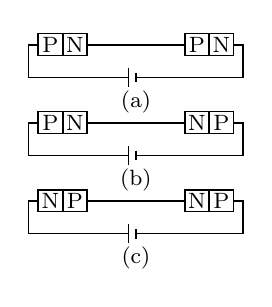
\begin{tikzpicture}[scale=0.62]
\foreach \y/\l/\a/\b/\c/\d in {0/(a)/P/N/P/N,-1.6/(b)/P/N/N/P,-3.2/(c)/N/P/N/P}{
\draw (0,\y) rectangle (0.5,\y+0.45) node[midway,lbl]{\a}; \draw (0.5,\y) rectangle (1,\y+0.45) node[midway,lbl]{\b};
\draw (1,\y+0.22) -- (3,\y+0.22);
\draw (3,\y) rectangle (3.5,\y+0.45) node[midway,lbl]{\c}; \draw (3.5,\y) rectangle (4,\y+0.45) node[midway,lbl]{\d};
\draw (0,\y+0.22) -- (-0.2,\y+0.22) -- (-0.2,\y-0.45) -- (1.85,\y-0.45); \draw (1.85,\y-0.25) -- (1.85,\y-0.65); \draw (2.0,\y-0.35) -- (2.0,\y-0.55);
\draw (2.0,\y-0.45) -- (4.2,\y-0.45) -- (4.2,\y+0.22) -- (4,\y+0.22); \node[lbl] at (2,\y-0.95) {\l};}
\end{tikzpicture}}
In the given circuits (a), (b) and (c), the potential drop across the two p-n junctions are equal in:\ntag{A}{335}{leph206}{13}{}{Class XII Part 2 \textperiodcentered{} Ch 14}}
{\opt{Both circuits (a) and (c)}{Circuit (a) only}{Circuit (b) only}{Circuit (c) only}}
\numoptstrue
\QQ{\qsrc{2022}{31}In half wave rectification, if the input frequency is $60\unit{Hz}$, then the output frequency would be:\ntag{D}{342}{leph206}{20}{ \textperiodcentered{} Exercise 14.6}{Class XII Part 2 \textperiodcentered{} Ch 14}}
{\opt{120\,Hz}{zero}{30\,Hz}{60\,Hz}}
\numoptstrue
\QQ{\qsrc{2020}{153}The increase in the width of the depletion region in a p-n junction diode is due to:\ntag{D}{336}{leph206}{14}{ \textperiodcentered{} reverse bias widens depletion region}{Class XII Part 2 \textperiodcentered{} Ch 14}}
{\opt{forward bias only}{reverse bias only}{both forward bias and reverse bias}{increase in forward current}}
\numoptstrue
\QQ{\qsrc{2018}{16}In a p-n junction diode, change in temperature due to heating\ntag{A}{337}{leph206}{15}{}{Class XII Part 2 \textperiodcentered{} Ch 14}}
{\opt{does not affect resistance of p-n junction}{affects only forward resistance}{affects only reverse resistance}{affects the overall V--I characteristics of p-n junction}}
\numoptstrue
\QQ{\qsrc{2017}{147}Which one of the following represents forward bias diode?\ntag{A}{334}{leph206}{12}{}{Class XII Part 2 \textperiodcentered{} Ch 14}}
{\opt{$-4$\,V\,\begin{circuitikz}[scale=0.5,transform shape,baseline=-2pt]\draw (0,0) to[empty diode] (1.5,0) to[R] (3,0);\end{circuitikz}\,$-3$\,V}{$-2$\,V\,\begin{circuitikz}[scale=0.5,transform shape,baseline=-2pt]\draw (0,0) to[empty diode] (1.5,0) to[R] (3,0);\end{circuitikz}\,$+2$\,V}{3\,V\,\begin{circuitikz}[scale=0.5,transform shape,baseline=-2pt]\draw (0,0) to[empty diode] (1.5,0) to[R] (3,0);\end{circuitikz}\,5\,V}{0\,V\,\begin{circuitikz}[scale=0.5,transform shape,baseline=-2pt]\draw (0,0) to[empty diode] (1.5,0) to[R] (3,0);\end{circuitikz}\,$-2$\,V}}
\numoptstrue
\QQ{\qsrc{2016}{13}Consider the junction diode as ideal. The value of current flowing through AB is:
\fig{\begin{circuitikz}[scale=0.62,transform shape,font=\Large]
\draw (0,0) node[circ]{} node[above]{A} node[below]{$+4$\,V} to[empty diode] (2,0) to[R,l=1\,k$\Omega$] (4.4,0) node[circ]{} node[above]{B} node[below]{$-6$\,V};
\end{circuitikz}}\ntag{A}{334}{leph206}{12}{ \textperiodcentered{} forward bias}{Class XII Part 2 \textperiodcentered{} Ch 14}}
{\opt{0\,A}{$10^{-2}$\,A}{$10^{-1}$\,A}{$10^{-3}$\,A}}
\end{multicols}
\par\needspace{12\baselineskip}\vspace{12pt}
\begin{center}{\pgfornament[width=3.2cm,color=gilt]{87}}\par
{\large\color{navy}\scshape Semiconductor Electronics \textperiodcentered{} Answer Key}\end{center}
{\small\setlength{\tabcolsep}{1pt}\renewcommand{\arraystretch}{1.5}
\begin{tabularx}{\linewidth}{@{}*{8}{>{\centering\arraybackslash}X}@{}}\toprule
\textbf{1}\,(3) & \textbf{2}\,(2) & \textbf{3}\,(3) & \textbf{4}\,(1)$^{*}$ & \textbf{5}\,(4) & \textbf{6}\,(1) & \textbf{7}\,(4) & \textbf{8}\,(2)\\
\textbf{9}\,(4) & \textbf{10}\,(4) & \textbf{11}\,(2) &  &  &  &  & \\\bottomrule\end{tabularx}}\par\smallskip
{\footnotesize Answers of 2021, 2022, 2023, 2025 and 2026 are from the official NTA final keys (checked by the editor); answers of 2016--2020 and 2024 were solved by the editor. $^{*}$: see note.
\par\smallskip\textbf{4.} (NEET 2025 Q40) The official NTA key accepts both (1) and (2).
}\par
\par\needspace{18\baselineskip}\vspace{14pt}
\begin{center}{\pgfornament[width=3.2cm,color=gilt]{87}}\par
{\large\color{navy}\scshape Chapter Summary \textperiodcentered{} Semiconductor Electronics}\end{center}
{\small\setlength{\tabcolsep}{3.5pt}
\begin{tabular*}{\linewidth}{@{\extracolsep{\fill}}l*{11}{c}c@{}}\toprule
Year & 2016 & 2017 & 2018 & 2019 & 2020 & 2021 & 2022 & 2023 & 2024 & 2025 & 2026 & Total\\\midrule
Questions & 1 & 1 & 1 & 1 & 1 & 1 & 2 & 1 & 0 & 1 & 1 & \textbf{11}\\\bottomrule\end{tabular*}}\par\medskip
{\small\textbf{\color{crimson}Topic-wise} (in textbook order)\par\smallskip
\begin{tabularx}{\linewidth}{@{}>{\raggedright\arraybackslash}Xrrrl@{}}\toprule
Topic & Qs & Direct & Years & 2016 $\rightarrow$ 2026\\\midrule
Semiconductors (intrinsic, extrinsic, bands) & \textbf{2} & 1 & 2 & {\scriptsize {\color{gray!45}16} {\color{gray!45}17} {\color{gray!45}18} \textbf{19} {\color{gray!45}20} \textbf{21} {\color{gray!45}22} {\color{gray!45}23} {\color{gray!45}24} {\color{gray!45}25} {\color{gray!45}26}}\\
p-n junction diode and rectifier & \textbf{9} & 3 & 8 & {\scriptsize \textbf{16} \textbf{17} \textbf{18} {\color{gray!45}19} \textbf{20} {\color{gray!45}21} \textbf{22} \textbf{23} {\color{gray!45}24} \textbf{25} \textbf{26}}\\
\bottomrule\end{tabularx}}\par\medskip
\begin{minipage}[t]{0.34\linewidth}{\small\textbf{\color{crimson}Direct vs Applied}\par\smallskip
\begin{tabular}{@{}lrr@{}}\toprule
Direct from NCERT & \textbf{4} & 36\%\\
\quad text, table, figure & 2 &\\
\quad solved Example & 0 &\\
\quad Exercise & 2 &\\
Applied & \textbf{7} & 64\%\\\midrule
Easy / Mod. / Hard & \multicolumn{2}{r}{7 / 4 / 0}\\\bottomrule
\end{tabular}}\end{minipage}\hfill
\begin{minipage}[t]{0.63\linewidth}{\small\textbf{\color{crimson}What to focus on}\par\smallskip
\begin{itemize}[leftmargin=1.1em,itemsep=1pt,topsep=0pt]
\item 11 questions in 11 papers, about 1.0 per paper; rank 23 of 28 chapters by number of questions.
\item Most asked topic: \textbf{p-n junction diode and rectifier} (9 questions, in 8 of the 11 years).
\item Asked in 8 or more of the 11 years: p-n junction diode and rectifier.
\item 2 questions are NCERT solved Examples or Exercises: Exercise 14.2 (Q 2), Exercise 14.6 (Q 7). Work these by hand.
\item Difficulty: 7 easy, 4 moderate, 0 hard.
\item 7 applied questions: practise these after the NCERT Examples and Exercises of the chapter.
\end{itemize}}\end{minipage}\par
\chapterpaper{Outside the 2026-27 Syllabus}{Deleted Portions}{58 questions \textperiodcentered{} topics removed from the rationalised NCERT}{cdeleted}{Deleted Portions}
{\small These questions were asked on topics that are no longer in the 2026-27 NCERT textbooks; 6 of them are from 2025 and 2026. They are kept here for completeness; a student following the present syllabus can skip this section. Topics are in order of how often they were asked.}\par\medskip
\begin{multicols}{2}
\topichead{Digital electronics (logic gates)}{11}
\numoptstrue
\QQ{\qsrc{2025}{8}The output (Y) of the given logic implementation is similar to the output of an/a \rule{1.2cm}{0.4pt} gate.
\fig{\begin{circuitikz}[scale=0.7,transform shape]
\draw (0,1.2) node[nor port](G1){}; \draw (0,-0.6) node[nand port](G2){}; \draw (2.4,0.3) node[and port](G3){};
\draw (G1.in 1) -- ++(-0.5,0) node[ocirc]{} node[left]{A};
\draw (G2.in 2) -- ++(-0.5,0) node[ocirc]{} node[left]{A};
\draw (G1.in 2) -- ++(-0.3,0) coordinate(b1); \draw (G2.in 1) -- ++(-0.3,0) coordinate(b2); \draw (b1) -- (b2);
\draw ($(b1)!0.5!(b2)$) -- ++(-0.4,0) node[ocirc]{} node[left]{B};
\draw (G1.out) -| (G3.in 1); \draw (G2.out) -| (G3.in 2);
\draw (G3.out) -- ++(0.4,0) node[ocirc]{} node[right]{Y};
\end{circuitikz}}\ntag{X}{}{}{}{}{digital electronics (logic gates)}}
{\opt{AND}{NAND}{OR}{NOR}}
\numoptstrue
\QQ{\qsrc{2024}{11}The output ($Y$) of the given logic gate is similar to the output of an/a:
\fig{\begin{circuitikz}[scale=0.7,transform shape]
\draw (0,1.0) node[nand port](G1){}; \draw (0,-0.6) node[nor port](G2){}; \draw (2.5,0.2) node[nor port](G3){};
\draw (G1.in 1) -- ++(-0.3,0) coordinate(a1); \draw (G1.in 2) -- ++(-0.3,0) coordinate(a2); \draw (a1) -- (a2); \draw ($(a1)!0.5!(a2)$) -- ++(-0.4,0) node[left]{$A$};
\draw (G2.in 1) -- ++(-0.3,0) coordinate(b1); \draw (G2.in 2) -- ++(-0.3,0) coordinate(b2); \draw (b1) -- (b2); \draw ($(b1)!0.5!(b2)$) -- ++(-0.4,0) node[left]{$B$};
\draw (G1.out) -| (G3.in 1); \draw (G2.out) -| (G3.in 2); \draw (G3.out) -- ++(0.4,0) node[right]{$Y$};
\end{circuitikz}}\ntag{X}{}{}{}{}{digital electronics (logic gates)}}
{\opt{AND gate}{NAND gate}{NOR gate}{OR gate}}
\numoptstrue
\QQ{\qsrc{2024}{16}A logic circuit provides the output $Y$ as per the following truth table:\par\smallskip
{\centering\begin{tabular}{|c|c|c|}\hline $A$ & $B$ & $Y$\\\hline 0 & 0 & 1\\ 0 & 1 & 0\\ 1 & 0 & 1\\ 1 & 1 & 0\\\hline\end{tabular}\par}\smallskip
The expression for the output $Y$ is:\ntag{X}{}{}{}{}{digital electronics (logic gates)}}
{\opt{$B$}{$A\cdot B+\bar A$}{$A\cdot\bar B+\bar A$}{$\bar B$}}
\numoptstrue
\QQ{\qsrc{2023}{39}For the following logic circuit, the truth table is:
\fig{\begin{circuitikz}[scale=0.7,transform shape]
\draw (0,1) node[not port](N1){}; \draw (0,-0.6) node[not port](N2){}; \draw (2.2,0.2) node[nand port](G){};
\draw (N1.in) -- ++(-0.5,0) node[left]{A}; \draw (N2.in) -- ++(-0.5,0) node[left]{B};
\draw (N1.out) -| (G.in 1); \draw (N2.out) -| (G.in 2); \draw (G.out) -- ++(0.4,0) node[right]{Y};
\end{circuitikz}}\ntag{X}{}{}{}{}{digital electronics (logic gates)}}
{\opt{\ttab{0&0&0}{0&1&0}{1&0&0}{1&1&1}}{\ttab{0&0&1}{0&1&1}{1&0&1}{1&1&0}}{\ttab{0&0&0}{0&1&1}{1&0&1}{1&1&1}}{\ttab{0&0&1}{0&1&0}{1&0&1}{1&1&0}}}
\numoptstrue
\QQ{\qsrc{2022}{44}\fig{\begin{circuitikz}[scale=0.7,transform shape]
\draw (0,1.0) node[nand port](G1){}; \draw (0,-0.8) node[nand port](G2){}; \draw (2.6,0.1) node[and port](G3){};
\draw (G1.in 1) -- ++(-2.2,0) coordinate(A0) node[left]{A}; \draw (G2.in 2) -- ++(-2.2,0) node[left]{B};
\draw (G1.in 2) -- ++(-0.4,0) |- ($(G2.in 2)+(-0.4,0)$);
\draw ($(A0)+(0.5,0)$) node[circ]{} |- ++(0,-0.9) coordinate(nin); \draw (nin) -- ++(0.1,0) node[not port,anchor=in,scale=0.6](N){}; \draw (N.out) |- (G2.in 1);
\draw (G1.out) -| (G3.in 1); \draw (G2.out) -| (G3.in 2); \draw (G3.out) -- ++(0.4,0) node[right]{C};
\end{circuitikz}}
The truth table for the given logic circuit is:\ntag{X}{}{}{}{}{digital electronics (logic gates)}}
{\opt{\ttab{0&0&0}{0&1&1}{1&0&0}{1&1&1}}{\ttab{0&0&0}{0&1&1}{1&0&1}{1&1&0}}{\ttab{0&0&1}{0&1&0}{1&0&0}{1&1&1}}{\ttab{0&0&1}{0&1&0}{1&0&1}{1&1&0}}}
\numoptstrue
\QQ{\qsrc{2021}{38}For the given circuit, the input digital signals are applied at the terminals A, B and C. What would be the output at the terminal $y$?
\fig{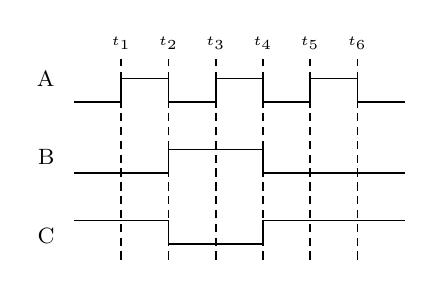
\begin{tikzpicture}[xscale=0.6,yscale=0.5]
\foreach \x/\l in {1/t_1,2/t_2,3/t_3,4/t_4,5/t_5,6/t_6} {\draw[densely dashed] (\x,-4.6) -- (\x,0.5); \node[font=\tiny] at (\x,0.9) {$\l$};}
\node[lbl,left] at (-0.2,0) {A}; \draw (0,-0.6) -- (1,-0.6) -- (1,0) -- (2,0) -- (2,-0.6) -- (3,-0.6) -- (3,0) -- (4,0) -- (4,-0.6) -- (5,-0.6) -- (5,0) -- (6,0) -- (6,-0.6) -- (7,-0.6);
\node[lbl,left] at (-0.2,-2) {B}; \draw (0,-2.4) -- (2,-2.4) -- (2,-1.8) -- (4,-1.8) -- (4,-2.4) -- (7,-2.4);
\node[lbl,left] at (-0.2,-4) {C}; \draw (0,-3.6) -- (2,-3.6) -- (2,-4.2) -- (4,-4.2) -- (4,-3.6) -- (7,-3.6);
\end{tikzpicture}}
\fig{\begin{circuitikz}[scale=0.75,transform shape]
\draw (0,1) node[and port](G1){}; \draw (0,-1) node[nand port](G2){}; \draw (2.4,0) node[or port](G3){};
\draw (G1.in 1) -- ++(-0.8,0) node[ocirc]{} node[left]{A}; \draw (G2.in 2) -- ++(-0.8,0) node[ocirc]{} node[left]{C};
\draw (G1.in 2) -- ++(-0.4,0) |- (G2.in 1); \draw ($(G1.in 2)+(-0.4,-1)$) -- ++(-0.4,0) node[ocirc]{} node[left]{B};
\draw (G1.out) -| (G3.in 1); \draw (G2.out) -| (G3.in 2); \draw (G3.out) -- ++(0.4,0) node[ocirc]{} node[right]{$y$};
\end{circuitikz}}\ntag{X}{}{}{}{}{digital electronics (logic gates)}}
{\optfig{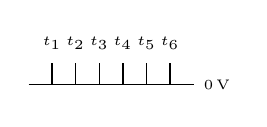
\begin{tikzpicture}[xscale=0.3,yscale=0.35]\foreach \x in {1,...,6} \node[font=\tiny] at (\x,1.5) {$t_\x$};\draw (0,0) -- (7,0) node[right,font=\tiny]{0\,V}; \foreach \x in {1,6} \draw (\x,0) -- (\x,0.8); \foreach \x in {2,...,5} \draw[thin] (\x,0) -- (\x,0.8);\end{tikzpicture}}{\begin{tikzpicture}[xscale=0.3,yscale=0.35]\foreach \x in {1,...,6} \node[font=\tiny] at (\x,1.5) {$t_\x$};\draw (0,0) -- (1,0) -- (1,1) -- (3,1) -- (3,0) -- (6,0) -- (6,1) -- (7,1) node[right,font=\tiny]{5\,V};\end{tikzpicture}}{\begin{tikzpicture}[xscale=0.3,yscale=0.35]\foreach \x in {1,...,6} \node[font=\tiny] at (\x,1.5) {$t_\x$};\draw (0,1) -- (7,1) node[right,font=\tiny]{5\,V};\end{tikzpicture}}{\begin{tikzpicture}[xscale=0.3,yscale=0.35]\foreach \x in {1,...,6} \node[font=\tiny] at (\x,1.5) {$t_\x$};\draw (0,1) -- (1,1) -- (1,0) -- (3,0) -- (3,1) -- (6,1) -- (6,0) -- (7,0) node[right,font=\tiny]{0\,V};\end{tikzpicture}}}
\numoptstrue
\QQ{\qsrc{2020}{180}For the logic circuit shown, the truth table is:
\fig{\begin{circuitikz}[scale=0.7,transform shape]
\draw (0,1) node[not port](N1){}; \draw (0,-0.6) node[not port](N2){}; \draw (2.2,0.2) node[nor port](G){};
\draw (N1.in) -- ++(-0.5,0) node[left]{A}; \draw (N2.in) -- ++(-0.5,0) node[left]{B};
\draw (N1.out) -| (G.in 1); \draw (N2.out) -| (G.in 2); \draw (G.out) -- ++(0.4,0) node[right]{Y};
\end{circuitikz}}\ntag{X}{}{}{}{}{digital electronics (logic gates)}}
{\opt{\ttab{0&0&0}{0&1&0}{1&0&0}{1&1&1}}{\ttab{0&0&0}{0&1&1}{1&0&1}{1&1&1}}{\ttab{0&0&1}{0&1&1}{1&0&1}{1&1&0}}{\ttab{0&0&1}{0&1&0}{1&0&0}{1&1&0}}}
\numoptstrue
\QQ{\qsrc{2019}{39}\fig{\begin{circuitikz}[scale=0.6,transform shape,font=\Large]
\draw (4,4) node[circ]{} node[right]{$+6$\,V} to[R,l=R] (4,2.4) node[circ]{}; \draw (4,2.4) -- (4.6,2.4) node[right]{LED (Y)};
\draw (4,2.4) to[R,l=R] (4,0.8) -- (4,0.4) node[ground]{};
\draw (1,3.2) node[left]{0} (1,2.4) node[below left]{A\ 1}; \draw (1,2.4) -- (4,2.4); \draw (1.1,2.45) -- (1.6,3.0);
\draw (1,1.2) node[left]{0} (1,0.8) node[below left]{B\ 1}; \draw (1,0.8) -- (4,0.8); \draw (1.1,0.85) -- (1.6,1.4);
\draw (0.6,2.4) -- (0.6,0.8);
\end{circuitikz}}
The \textbf{correct} Boolean operation represented by the circuit diagram drawn is:\ntag{X}{}{}{}{}{digital electronics (logic gates)}}
{\opt{AND}{OR}{NAND}{NOR}}
\numoptstrue
\QQ{\qsrc{2018}{17}In the combination of the following gates the output Y can be written in terms of inputs A and B as
\fig{\begin{circuitikz}[scale=0.7,transform shape]
\draw (3,1.2) node[and port](G1){}; \draw (3,-1.0) node[and port](G2){}; \draw (5.2,0.1) node[or port](G3){};
\draw (0,1.6) node[circ]{} node[left]{A} -- (0.6,1.6) coordinate(a1); \draw (a1) |- (G1.in 1);
\draw (a1) |- (1.0,-0.8) node[not port,anchor=in,scale=0.6](N2){}; \draw (N2.out) -| ($(G2.in 1)+(-0.2,0)$) -- (G2.in 1);
\draw (0,-1.6) node[circ]{} node[left]{B} -- (0.3,-1.6) coordinate(b1); \draw (b1) |- (G2.in 2);
\draw (b1) |- (1.0,1.0) node[not port,anchor=in,scale=0.6](N1){}; \draw (N1.out) -| ($(G1.in 2)+(-0.2,0)$) -- (G1.in 2);
\draw (G1.out) -| (G3.in 1); \draw (G2.out) -| (G3.in 2); \draw (G3.out) -- ++(0.4,0) node[circ]{} node[right]{Y};
\end{circuitikz}}\ntag{X}{}{}{}{}{digital electronics (logic gates)}}
{\opt{$\overline{A\cdot B}+A\cdot B$}{$A\cdot\bar B+\bar A\cdot B$}{$\overline{A\cdot B}$}{$\overline{A+B}$}}
\numoptstrue
\QQ{\qsrc{2017}{142}The given electrical network is equivalent to:
\fig{\begin{circuitikz}[scale=0.7,transform shape]
\draw (0,0) node[nor port](G1){}; \draw (2.6,0) node[nor port](G2){}; \draw (4.6,0) node[not port](N){};
\draw (G1.in 1) -- ++(-0.4,0) node[circ]{} node[left]{A}; \draw (G1.in 2) -- ++(-0.4,0) node[circ]{} node[left]{B};
\draw (G1.out) -- ++(0.3,0) coordinate(m); \draw (m) |- (G2.in 1); \draw (m) |- (G2.in 2); \draw (G2.out) -- (N.in); \draw (N.out) -- ++(0.3,0) node[circ]{} node[above]{Y};
\end{circuitikz}}\ntag{X}{}{}{}{}{digital electronics (logic gates)}}
{\opt{OR gate}{NOR gate}{NOT gate}{AND gate}}
\numoptstrue
\QQ{\qsrc{2016}{34}To get output 1 for the following circuit, the correct choice for the input is:
\fig{\begin{circuitikz}[scale=0.7,transform shape]
\draw (0,0.6) node[or port](G1){}; \draw (2.4,0.1) node[and port](G2){};
\draw (G1.in 1) -- ++(-0.5,0) node[ocirc]{} node[left]{A}; \draw (G1.in 2) -- ++(-0.5,0) node[ocirc]{} node[left]{B};
\draw (G1.out) -| (G2.in 1); \draw (G2.in 2) -- ++(-3.2,0) node[ocirc]{} node[left]{C}; \draw (G2.out) -- ++(0.5,0) node[ocirc]{} node[below]{Y};
\end{circuitikz}}\ntag{X}{}{}{}{}{digital electronics (logic gates)}}
{\opt{A = 0, B = 1, C = 0}{A = 1, B = 0, C = 0}{A = 1, B = 1, C = 0}{A = 1, B = 0, C = 1}}
\topichead{Brewster's law}{4}
\numoptstrue
\QQ{\qsrc{2025}{27}An unpolarized light beam travelling in air is incident on a medium of refractive index 1.73 at Brewster's angle. Then\ntag{X}{}{}{}{}{Brewster's law}}
{\opt{reflected light is completely polarized and the angle of reflection is close to $60^\circ$}{reflected light is partially polarized and the angle of reflection is close to $30^\circ$}{both reflected and transmitted light are perfectly polarized with angles of reflection and refraction close to $60^\circ$ and $30^\circ$, respectively}{transmitted light is completely polarized with angle of refraction close to $30^\circ$}}
\numoptstrue
\QQ{\qsrc{2024}{4}An unpolarised light beam strikes a glass surface at Brewster's angle. Then\ntag{X}{}{}{}{}{Brewster's law}}
{\opt{the reflected light will be completely polarised but the refracted light will be partially polarised.}{the reflected light will be partially polarised.}{the refracted light will be completely polarised.}{both the reflected and refracted light will be completely polarised.}}
\numoptstrue
\QQ{\qsrc{2020}{138}The Brewster's angle $i_b$ for an interface should be:\ntag{X}{}{}{}{}{Brewster's law}}
{\opt{$0^\circ<i_b<30^\circ$}{$30^\circ<i_b<45^\circ$}{$45^\circ<i_b<90^\circ$}{$i_b = 90^\circ$}}
\numoptstrue
\QQ{\qsrc{2018}{8}Unpolarised light is incident from air on a plane surface of a material of refractive index `$\mu$'. At a particular angle of incidence `$i$', it is found that the reflected and refracted rays are perpendicular to each other. Which of the following options is correct for this situation?\ntag{X}{}{}{}{}{Brewster's law}}
{\opt{$i = \sin^{-1}\!\left(\dfrac1\mu\right)$}{Reflected light is polarised with its electric vector perpendicular to the plane of incidence}{Reflected light is polarised with its electric vector parallel to the plane of incidence}{$i = \tan^{-1}\!\left(\dfrac1\mu\right)$}}
\topichead{Radioactive decay law (half-life, mean life, activity)}{4}
\numoptstrue
\QQ{\qsrc{2023}{28}The half life of a radioactive substance is 20 minutes. In how much time, the activity of substance drops to $\left(\frac1{16}\right)^{\text{th}}$ of its initial value?\ntag{X}{}{}{}{}{radioactive decay law (half-life)}}
{\opt{80 minutes}{20 minutes}{40 minutes}{60 minutes}}
\numoptstrue
\QQ{\qsrc{2021}{34}The half-life of a radioactive nuclide is 100 hours. The fraction of original activity that will remain after 150 hours would be:\ntag{X}{}{}{}{}{radioactive decay law (half-life)}}
{\opt{1/2}{$\dfrac1{2\sqrt2}$}{$\dfrac23$}{$\dfrac2{3\sqrt2}$}}
\numoptstrue
\QQ{\qsrc{2018}{13}For a radioactive material, half-life is 10 minutes. If initially there are 600 number of nuclei, the time taken (in minutes) for the disintegration of 450 nuclei is\ntag{X}{}{}{}{}{radioactive decay law (half-life)}}
{\opt{30}{10}{20}{15}}
\numoptstrue
\QQ{\qsrc{2017}{141}Radioactive material `A' has decay constant `$8\lambda$' and material `B' has decay constant `$\lambda$'. Initially they have same number of nuclei. After what time, the ratio of number of nuclei of material `B' to that `A' will be $\dfrac1e$?\ntag{X}{}{}{}{}{radioactive decay law (decay constant)}}
{\opt{$\dfrac1{7\lambda}$}{$\dfrac1{8\lambda}$}{$\dfrac1{9\lambda}$}{$\dfrac1\lambda$}}
\topichead{Transistor (incl. amplifier)}{4}
\numoptstrue
\QQ{\qsrc{2020}{156}For transistor action, which of the following statements is \textbf{correct}?\ntag{X}{}{}{}{}{transistor}}
{\opt{Base, emitter and collector regions should have same doping concentrations.}{Base, emitter and collector regions should have same size.}{Both emitter junction as well as the collector junction are forward biased.}{The base region must be very thin and lightly doped.}}
\numoptstrue
\QQ{\qsrc{2018}{15}In the circuit shown in the figure, the input voltage $V_i$ is 20\,V, $V_{BE} = 0$ and $V_{CE} = 0$. The values of $I_B$, $I_C$ and $\beta$ are given by
\fig{\begin{circuitikz}[scale=0.62,transform shape,font=\Large]
\draw (3,0) node[npn](Q){}; \draw (Q.B) to[R,l_={$R_B$ 500\,k$\Omega$}] ++(-2.4,0) node[circ]{} node[left]{$V_i$};
\draw (Q.C) to[R,l_={$R_C$ 4\,k$\Omega$}] ++(0,2) node[circ]{} node[above]{20\,V}; \draw (Q.E) -- ++(0,-0.4) node[ground]{};
\end{circuitikz}}\ntag{X}{}{}{}{}{transistor}}
{\opt{$I_B = 20\unit{\mu A}$, $I_C = 5\unit{mA}$, $\beta = 250$}{$I_B = 25\unit{\mu A}$, $I_C = 5\unit{mA}$, $\beta = 200$}{$I_B = 40\unit{\mu A}$, $I_C = 10\unit{mA}$, $\beta = 250$}{$I_B = 40\unit{\mu A}$, $I_C = 5\unit{mA}$, $\beta = 125$}}
\numoptstrue
\QQ{\qsrc{2017}{138}In a common emitter transistor amplifier the audio signal voltage across the collector is 3\,V. The resistance of collector is $3\unit{k\Omega}$. If current gain is 100 and the base resistance is $2\unit{k\Omega}$, the voltage and power gain of the amplifier is:\ntag{X}{}{}{}{}{transistor (CE amplifier)}}
{\opt{15 and 200}{150 and 15000}{20 and 2000}{200 and 1000}}
\numoptstrue
\QQ{\qsrc{2016}{17}A npn transistor is connected in common emitter configuration in a given amplifier. A load resistance of $800\unit{\Omega}$ is connected in the collector circuit and the voltage drop across it is 0.8\,V. If the current amplification factor is 0.96 and the input resistance of the circuit is $192\unit{\Omega}$, the voltage gain and the power gain of the amplifier will respectively be:\ntag{X}{}{}{}{}{transistor (CE amplifier)}}
{\opt{4, 3.84}{3.69, 3.84}{4, 4}{4, 3.69}}
\topichead{Alpha- and beta-decay}{3}
\numoptstrue
\QQ{\qsrc{2024}{28}${}^{290}_{\ 82}X\xrightarrow{\ \alpha\ }Y\xrightarrow{\ e^+\ }Z\xrightarrow{\ \beta^-\ }P\xrightarrow{\ e^-\ }Q$. In the nuclear emission stated above, the mass number and atomic number of the product Q respectively, are:\ntag{X}{}{}{}{}{alpha- and beta-decay}}
{\opt{286, 81}{280, 81}{286, 80}{288, 82}}
\numoptstrue
\QQ{\qsrc{2022}{11}In the given nuclear reaction, the element X is:
\[{}^{22}_{11}\mathrm{Na}\longrightarrow\mathrm X+e^++\nu\]\ntag{X}{}{}{}{}{alpha- and beta-decay}}
{\opt{${}^{22}_{12}$Mg}{${}^{23}_{11}$Na}{${}^{23}_{10}$Ne}{${}^{22}_{10}$Ne}}
\numoptstrue
\QQ{\qsrc{2021}{19}A radioactive nucleus ${}^A_Z$X undergoes spontaneous decay in the sequence ${}^A_Z\mathrm X\to{}_{Z-1}\mathrm B\to{}_{Z-3}\mathrm C\to{}_{Z-2}\mathrm D$, where $Z$ is the atomic number of element X. The possible decay particles in the sequence are:\ntag{X}{}{}{}{}{alpha- and beta-decay}}
{\opt{$\alpha$, $\beta^-$, $\beta^+$}{$\alpha$, $\beta^+$, $\beta^-$}{$\beta^+$, $\alpha$, $\beta^-$}{$\beta^-$, $\alpha$, $\beta^+$}}
\topichead{Parallel axis theorem}{3}
\numoptstrue
\QQ{\qsrc{2026}{27}A solid sphere A of radius $R$ and mass $M$ is attached at a point to a smaller solid sphere B of radius $r<R$ and mass $m<M$. Assume that the line joining their centres lies along the horizontal. The moment of inertia of the system calculated about a vertical axis passing through the centre of A is $I_A$ and that calculated about a vertical axis passing through the centre of B is $I_B$. The difference $I_A-I_B$ is:
\fig{\begin{tikzpicture}[scale=0.65]
\draw (0,0) circle (1); \draw (1.35,0) circle (0.35); \draw[densely dashed] (0,-1.5) -- (0,1.5) node[right,lbl]{$I_A$}; \draw[densely dotted] (0,0) -- (1.35,0);
\node[lbl] at (-1.15,0.75) {A}; \node[lbl] at (1.8,0.45) {B};
\begin{scope}[xshift=4.2cm]
\draw (0,0) circle (1); \draw (1.35,0) circle (0.35); \draw[densely dashed] (1.35,-1.5) -- (1.35,1.5) node[right,lbl]{$I_B$}; \draw[densely dotted] (0,0) -- (1.35,0);
\node[lbl] at (-1.15,0.75) {A}; \node[lbl] at (1.8,0.45) {B};
\end{scope}
\end{tikzpicture}}\ntag{X}{}{}{}{}{parallel axis theorem}}
{\opt{$(M-m)(R+r)^2$}{$(m-M)(R+r)^2$}{$(m-M)(R-r)^2$}{0}}
\numoptstrue
\QQ{\qsrc{2025}{39}A sphere of radius $R$ is cut from a larger solid sphere of radius $2R$ as shown in the figure. The ratio of the moment of inertia of the smaller sphere to that of the rest part of the sphere about the Y-axis is:
\fig{\begin{tikzpicture}[scale=0.6]
\fill[pattern=horizontal lines] (0,0) circle (2); \draw (0,0) circle (2);
\fill[white] (1,0) circle (1); \draw (1,0) circle (1);
\draw[->] (0,-2.4) -- (0,2.5) node[above,lbl]{Y}; \draw[->] (-2.4,0) -- (2.7,0) node[right,lbl]{X};
\draw[<->] (0,-0.25) -- (2,-0.25) node[midway,below,lbl]{$2R$};
\end{tikzpicture}}\ntag{X}{}{}{}{}{parallel axis theorem}}
{\opt{$\dfrac78$}{$\dfrac7{40}$}{$\dfrac7{57}$}{$\dfrac7{64}$}}
\numoptstrue
\QQ{\qsrc{2016}{1}From a disc of radius $R$ and mass $M$, a circular hole of diameter $R$, whose rim passes through the centre is cut. What is the moment of inertia of the remaining part of the disc about a perpendicular axis, passing through the centre?\ntag{X}{}{}{}{}{parallel axis theorem}}
{\opt{$15MR^2/32$}{$13MR^2/32$}{$11MR^2/32$}{$9MR^2/32$}}
\topichead{Potentiometer}{3}
\numoptstrue
\QQ{\qsrc{2021}{27}In a potentiometer circuit a cell of EMF 1.5\,V gives balance point at $36\unit{cm}$ length of wire. If another cell of EMF 2.5\,V replaces the first cell, then at what length of the wire, the balance point occurs?\ntag{X}{}{}{}{}{potentiometer}}
{\opt{60\,cm}{21.6\,cm}{64\,cm}{62\,cm}}
\numoptstrue
\QQ{\qsrc{2017}{150}A potentiometer is an accurate and versatile device to make electrical measurements of E.M.F.\ because the method involves:\ntag{X}{}{}{}{}{potentiometer}}
{\opt{potential gradients}{a condition of no current flow through the galvanometer}{a combination of cells, galvanometer and resistances}{cells}}
\numoptstrue
\QQ{\qsrc{2016}{31}A potentiometer wire is $100\unit{cm}$ long and a constant potential difference is maintained across it. Two cells are connected in series first to support one another and then in opposite direction. The balance points are obtained at $50\unit{cm}$ and $10\unit{cm}$ from the positive end of the wire in the two cases. The ratio of emf's is:\ntag{X}{}{}{}{}{potentiometer}}
{\opt{5:1}{5:4}{3:4}{3:2}}
\topichead{Resistor colour code}{3}
\numoptstrue
\QQ{\qsrc{2023}{18}Resistance of a carbon resistor determined from colour codes is $(22000\pm5\%)\unit{\Omega}$. The colour of third band must be:\ntag{X}{}{}{}{}{resistor colour code}}
{\opt{Yellow}{Red}{Green}{Orange}}
\numoptstrue
\QQ{\qsrc{2020}{164}The color code of a resistance is given below:
\fig{\begin{tikzpicture}[scale=0.7]
\draw (-0.6,0.5) -- (0,0.5); \draw (5,0.5) -- (5.6,0.5); \draw (0,0) rectangle (5,1);
\foreach \x/\c in {0.9/Yellow,1.9/Violet,2.9/Brown,3.9/Gold} {\fill (\x-0.15,0) rectangle (\x+0.15,1); \node[lbl,below] at (\x,0) {\c};}
\end{tikzpicture}}
The values of resistance and tolerance, respectively, are:\ntag{X}{}{}{}{}{resistor colour code}}
{\opt{470\,k$\Omega$, 5\%}{47\,k$\Omega$, 10\%}{4.7\,k$\Omega$, 5\%}{470\,$\Omega$, 5\%}}
\numoptstrue
\QQ{\qsrc{2018}{5}A carbon resistor of $(47\pm4.7)\unit{k\Omega}$ is to be marked with rings of different colours for its identification. The colour code sequence will be\ntag{X}{}{}{}{}{resistor colour code}}
{\opt{Yellow -- Green -- Violet -- Gold}{Yellow -- Violet -- Orange -- Silver}{Violet -- Yellow -- Orange -- Silver}{Green -- Orange -- Violet -- Gold}}
\topichead{Rolling motion}{3}
\numoptstrue
\QQ{\qsrc{2019}{9}A disc of radius $2\unit{m}$ and mass $100\unit{kg}$ rolls on a horizontal floor. Its centre of mass has speed of $20\unit{cm/s}$. How much work is needed to stop it?\ntag{X}{}{}{}{}{kinetic energy of rolling}}
{\opt{3\,J}{30\,kJ}{2\,J}{1\,J}}
\numoptstrue
\QQ{\qsrc{2018}{41}A solid sphere is in rolling motion. In rolling motion a body possesses translational kinetic energy ($K_t$) as well as rotational kinetic energy ($K_r$) simultaneously. The ratio $K_t:(K_t+K_r)$ for the sphere is\ntag{X}{}{}{}{}{kinetic energy of rolling}}
{\opt{10:7}{5:7}{7:10}{2:5}}
\numoptstrue
\QQ{\qsrc{2016}{21}A disk and a sphere of same radius but different masses roll off on two inclined planes of the same altitude and length. Which one of the two objects gets to the bottom of the plane first?\ntag{X}{}{}{}{}{kinetic energy of rolling}}
{\opt{Disk}{Sphere}{Both reach at the same time}{Depends on their masses}}
\topichead{Zener diode}{3}
\numoptstrue
\QQ{\qsrc{2026}{16}An ideal Zener diode with breakdown voltage of $-3\unit{V}$ is reverse biased with a negative input voltage $V_i = -5\unit{V}$. The magnitude of voltage difference between point B and A is:
\fig{\begin{circuitikz}[scale=0.62,transform shape,font=\Large]
\draw (0,2) node[circ]{} node[above]{C} to[zDo] (1.6,2) node[circ]{} node[above]{B} to[R,l=R] (3.6,2) node[circ]{} node[above]{A} -- (4.2,2) -- (4.2,0) to[battery1] (0,0) -- (0,2);
\end{circuitikz}}\ntag{X}{}{}{}{}{Zener diode}}
{\opt{3\,V}{2\,V}{1\,V}{0\,V}}
\numoptstrue
\QQ{\qsrc{2023}{16}Given below are two statements:\par
\textbf{Statement I}: Photovoltaic devices can convert optical radiation into electricity.\par
\textbf{Statement II}: Zener diode is designed to operate under reverse bias in breakdown region.\par
In the light of the above statements, choose the \textit{most appropriate} answer from the options given below:\ntag{X}{}{}{}{}{Zener diode}}
{\opt{Statement I is incorrect but Statement II is correct.}{Both Statement I and Statement II are correct.}{Both Statement I and Statement II are incorrect.}{Statement I is correct but Statement II is incorrect.}}
\numoptstrue
\QQ{\qsrc{2021}{1}Consider the following statements (A) and (B) and identify the correct answer.
\begin{stmts}[(\Alph*)]
\item A zener diode is connected in reverse bias, when used as a voltage regulator.
\item The potential barrier of p-n junction lies between 0.1\,V to 0.3\,V.
\end{stmts}\ntag{X}{}{}{}{}{Zener diode}}
{\opt{(A) and (B) both are correct.}{(A) and (B) both are incorrect.}{(A) is correct and (B) is incorrect.}{(A) is incorrect but (B) is correct.}}
\topichead{Doppler effect}{2}
\numoptstrue
\QQ{\qsrc{2017}{144}Two cars moving in opposite directions approach each other with speed of $22\unit{m/s}$ and $16.5\unit{m/s}$ respectively. The driver of the first car blows a horn having a frequency 400\,Hz. The frequency heard by the driver of the second car is [velocity of sound $340\unit{m/s}$]:\ntag{X}{}{}{}{}{Doppler effect}}
{\opt{361\,Hz}{411\,Hz}{448\,Hz}{350\,Hz}}
\numoptstrue
\QQ{\qsrc{2016}{4}A siren emitting a sound of frequency 800\,Hz moves away from an observer towards a cliff at a speed of $15\unit{m\,s^{-1}}$. Then, the frequency of sound that the observer hears in the echo reflected from the cliff is: (Take velocity of sound in air $= 330\unit{m\,s^{-1}}$)\ntag{X}{}{}{}{}{Doppler effect}}
{\opt{765\,Hz}{800\,Hz}{838\,Hz}{885\,Hz}}
\topichead{Earth's magnetism (incl. angle of dip)}{2}
\numoptstrue
\QQ{\qsrc{2019}{26}At a point A on the earth's surface the angle of dip, $\delta = +25^\circ$. At a point B on the earth's surface the angle of dip, $\delta = -25^\circ$. We can interpret that:\ntag{X}{}{}{}{}{Earth's magnetism (angle of dip)}}
{\opt{A and B are both located in the northern hemisphere.}{A is located in the southern hemisphere and B is located in the northern hemisphere.}{A is located in the northern hemisphere and B is located in the southern hemisphere.}{A and B are both located in the southern hemisphere.}}
\numoptstrue
\QQ{\qsrc{2017}{149}If $\theta_1$ and $\theta_2$ be the apparent angles of dip observed in two vertical planes at right angles to each other, then the true angle of dip $\theta$ is given by:\ntag{X}{}{}{}{}{Earth's magnetism (angle of dip)}}
{\opt{$\tan^2\theta = \tan^2\theta_1+\tan^2\theta_2$}{$\cot^2\theta = \cot^2\theta_1-\cot^2\theta_2$}{$\tan^2\theta = \tan^2\theta_1-\tan^2\theta_2$}{$\cot^2\theta = \cot^2\theta_1+\cot^2\theta_2$}}
\topichead{Resolving power (telescope, microscope)}{2}
\numoptstrue
\QQ{\qsrc{2020}{168}Assume that light of wavelength $600\unit{nm}$ is coming from a star. The limit of resolution of telescope whose objective has a diameter of $2\unit{m}$ is:\ntag{X}{}{}{}{}{resolving power of a telescope}}
{\opt{$3.66\times10^{-7}\unit{rad}$}{$1.83\times10^{-7}\unit{rad}$}{$7.32\times10^{-7}\unit{rad}$}{$6.00\times10^{-7}\unit{rad}$}}
\numoptstrue
\QQ{\qsrc{2017}{151}The ratio of resolving powers of an optical microscope for two wavelengths $\lambda_1 = 4000\unit{\text{\AA}}$ and $\lambda_2 = 6000\unit{\text{\AA}}$ is:\ntag{X}{}{}{}{}{resolving power of microscope}}
{\opt{9:4}{3:2}{16:81}{8:27}}
\topichead{Coefficient of restitution}{1}
\numoptstrue
\QQ{\qsrc{2018}{32}A moving block having mass $m$, collides with another stationary block having mass $4m$. The lighter block comes to rest after collision. When the initial velocity of the lighter block is $v$, then the value of coefficient of restitution ($e$) will be\ntag{X}{}{}{}{}{coefficient of restitution}}
{\opt{0.8}{0.25}{0.5}{0.4}}
\topichead{Eddy currents}{1}
\numoptstrue
\QQ{\qsrc{2019}{6}In which of the following devices, the eddy current effect is \textbf{not} used?\ntag{X}{}{}{}{}{eddy currents}}
{\opt{induction furnace}{magnetic braking in train}{electromagnet}{electric heater}}
\topichead{Force between capacitor plates}{1}
\numoptstrue
\QQ{\qsrc{2018}{23}The electrostatic force between the metal plates of an isolated parallel plate capacitor C having a charge Q and area A, is\ntag{X}{}{}{}{}{force between capacitor plates}}
{\opt{proportional to the square root of the distance between the plates.}{linearly proportional to the distance between the plates.}{independent of the distance between the plates.}{inversely proportional to the distance between the plates.}}
\topichead{Intensity of EM waves}{1}
\numoptstrue
\QQ{\qsrc{2020}{150}Light with an average flux of $20\unit{W/cm^2}$ falls on a non-reflecting surface at normal incidence having surface area $20\unit{cm^2}$. The energy received by the surface during time span of 1 minute is:\ntag{X}{}{}{}{}{intensity of EM waves}}
{\opt{$10\times10^3\unit{J}$}{$12\times10^3\unit{J}$}{$24\times10^3\unit{J}$}{$48\times10^3\unit{J}$}}
\topichead{Magnetic field of a finite straight wire}{1}
\numoptstrue
\QQ{\qsrc{2023}{44}A very long conducting wire is bent in a semi-circular shape from A to B as shown in figure. The magnetic field at point P for steady current configuration is given by:
\fig{\begin{tikzpicture}[scale=0.8]
\draw[densely dashed] (-2.6,0.9) -- (-1.4,0.9); \draw[->] (-1.4,0.9) -- (-0.6,0.9); \draw (-0.6,0.9) -- (0,0.9) node[right,lbl]{A}; \node[lbl] at (-0.9,1.2) {$i\rightarrow$};
\draw (0,0.9) arc (90:-90:0.9); \draw[->] (0.64,-0.64) -- (0.6,-0.67);
\draw (0,-0.9) node[right,lbl]{B} -- (-0.6,-0.9); \draw[->] (-0.6,-0.9) -- (-1.4,-0.9); \draw[densely dashed] (-1.4,-0.9) -- (-2.6,-0.9); \node[lbl] at (-0.9,-0.6) {$i\leftarrow$};
\fill (0,0) circle (1.3pt) node[right,lbl]{P}; \draw[->] (0,0) -- (130:0.9) node[pos=0.6,above right,lbl]{$R$};
\end{tikzpicture}}\ntag{X}{}{}{}{}{magnetic field of a finite straight wire}}
{\opt{$\dfrac{\mu_0i}{4R}\left[1-\dfrac2\pi\right]$ pointed into the page}{$\dfrac{\mu_0i}{4R}$ pointed into the page}{$\dfrac{\mu_0i}{4R}$ pointed away from the page}{$\dfrac{\mu_0i}{4R}\left[1-\dfrac2\pi\right]$ pointed away from page}}
\topichead{Oscillation period of a magnetic needle}{1}
\numoptstrue
\QQ{\qsrc{2024}{3}In a uniform magnetic field of $0.049\unit{T}$, a magnetic needle performs 20 complete oscillations in 5 seconds as shown. The moment of inertia of the needle is $9.8\times10^{-6}\unit{kg\,m^2}$. If the magnitude of magnetic moment of the needle is $x\times10^{-5}\unit{A\,m^2}$, then the value of $x$ is:
\fig{\begin{tikzpicture}[scale=0.8]
\fill[pattern=north east lines] (-0.6,1.2) rectangle (0.6,1.4); \draw (-0.6,1.2) -- (0.6,1.2); \draw (0,1.2) -- (0,0.15);
\draw[thick] (-0.7,-0.15) -- (0.7,0.15); \node[lbl] at (0.85,0.3) {N}; \node[lbl] at (-0.85,-0.3) {S};
\draw[densely dashed,->] (-1.2,0.4) -- (1.4,0.4); \draw[densely dashed,->] (-1.2,-0.4) -- (1.4,-0.4) node[right,lbl]{$B$};
\end{tikzpicture}}\ntag{X}{}{}{}{}{oscillation period of a magnetic needle}}
{\opt{$1280\pi^2$}{$5\pi^2$}{$128\pi^2$}{$50\pi^2$}}
\topichead{Rainbow}{1}
\numoptstrue
\QQ{\qsrc{2019}{15}Pick the \textbf{wrong} answer in the context with rainbow.\ntag{X}{}{}{}{}{rainbow}}
{\opt{When the light rays undergo two internal reflections in a water drop, a secondary rainbow is formed.}{The order of colours is reversed in the secondary rainbow.}{An observer can see a rainbow when his front is towards the sun.}{Rainbow is a combined effect of dispersion, refraction and reflection of sunlight.}}
\topichead{Sharpness of resonance (Q-factor)}{1}
\numoptstrue
\QQ{\qsrc{2021}{39}A series LCR circuit containing $5.0\unit{H}$ inductor, $80\unit{\mu F}$ capacitor and $40\unit{\Omega}$ resistor is connected to $230\unit{V}$ variable frequency ac source. The angular frequencies of the source at which power transferred to the circuit is half the power at the resonant angular frequency are likely to be:\ntag{X}{}{}{}{}{sharpness of resonance (half-power frequencies)}}
{\opt{25\,rad/s and 75\,rad/s}{50\,rad/s and 25\,rad/s}{46\,rad/s and 54\,rad/s}{42\,rad/s and 58\,rad/s}}
\topichead{Solar cell}{1}
\numoptstrue
\QQ{\qsrc{2024}{5}Consider the following statements A and B and identify the correct answer:
\fig{\begin{tikzpicture}[scale=0.7]
\draw[->] (-1.2,0) -- (1.4,0) node[right,lbl]{$V$}; \draw[->] (0,-0.9) -- (0,1.2) node[above,lbl]{$I$};
\node[lbl] at (0.5,0.45) {(I)}; \node[lbl] at (-0.55,0.45) {(II)}; \node[lbl] at (-0.55,-0.45) {(III)}; \node[lbl] at (0.5,-0.45) {(IV)};
\end{tikzpicture}}
\begin{stmts}[\Alph*.]
\item For a solar-cell, the I-V characteristics lies in the IV quadrant of the given graph.
\item In a reverse biased pn junction diode, the current measured in ($\mu$A), is due to majority charge carriers.
\end{stmts}\ntag{X}{}{}{}{}{solar cell (special purpose diodes)}}
{\opt{Both A and B are incorrect.}{A is correct but B is incorrect.}{A is incorrect but B is correct.}{Both A and B are correct.}}
\topichead{Types of errors}{1}
\numoptstrue
\QQ{\qsrc{2023}{23}The errors in the measurement which arise due to unpredictable fluctuations in temperature and voltage supply are:\ntag{X}{}{}{}{}{types of errors}}
{\opt{Random errors}{Instrumental errors}{Personal errors}{Least count errors}}
\topichead{Velocity selector}{1}
\numoptstrue
\QQ{\qsrc{2025}{3}An electron (mass $9\times10^{-31}\unit{kg}$ and charge $1.6\times10^{-19}\unit{C}$) moving with speed $c/100$ ($c$ = speed of light) is injected into a magnetic field $\vec B$ of magnitude $9\times10^{-4}\unit{T}$ perpendicular to its direction of motion. We wish to apply a uniform electric field $\vec E$ together with the magnetic field so that the electron does not deflect from its path. Then (speed of light $c = 3\times10^8\unit{m\,s^{-1}}$)\ntag{X}{}{}{}{}{velocity selector (crossed E and B)}}
{\opt{$\vec E$ is perpendicular to $\vec B$ and its magnitude is $27\times10^4\unit{V\,m^{-1}}$}{$\vec E$ is perpendicular to $\vec B$ and its magnitude is $27\times10^2\unit{V\,m^{-1}}$}{$\vec E$ is parallel to $\vec B$ and its magnitude is $27\times10^2\unit{V\,m^{-1}}$}{$\vec E$ is parallel to $\vec B$ and its magnitude is $27\times10^4\unit{V\,m^{-1}}$}}
\end{multicols}
\par\needspace{12\baselineskip}\vspace{12pt}
\begin{center}{\pgfornament[width=3.2cm,color=gilt]{87}}\par
{\large\color{navy}\scshape Deleted Portions \textperiodcentered{} Answer Key}\end{center}
{\small\setlength{\tabcolsep}{1pt}\renewcommand{\arraystretch}{1.5}
\begin{tabularx}{\linewidth}{@{}*{8}{>{\centering\arraybackslash}X}@{}}\toprule
\textbf{1}\,(4) & \textbf{2}\,(1) & \textbf{3}\,(4) & \textbf{4}\,(3) & \textbf{5}\,(4) & \textbf{6}\,(3) & \textbf{7}\,(1) & \textbf{8}\,(3)\\
\textbf{9}\,(2) & \textbf{10}\,(2) & \textbf{11}\,(4) & \textbf{12}\,(1) & \textbf{13}\,(1) & \textbf{14}\,(3) & \textbf{15}\,(2) & \textbf{16}\,(1)\\
\textbf{17}\,(2) & \textbf{18}\,(3) & \textbf{19}\,(1)$^{*}$ & \textbf{20}\,(4) & \textbf{21}\,(4) & \textbf{22}\,(2) & \textbf{23}\,(1) & \textbf{24}\,(1)\\
\textbf{25}\,(4) & \textbf{26}\,(3) & \textbf{27}\,(2) & \textbf{28}\,(3) & \textbf{29}\,(2) & \textbf{30}\,(1) & \textbf{31}\,(2) & \textbf{32}\,(4)\\
\textbf{33}\,(4) & \textbf{34}\,(4) & \textbf{35}\,(2) & \textbf{36}\,(1) & \textbf{37}\,(2) & \textbf{38}\,(2) & \textbf{39}\,(2) & \textbf{40}\,(2)\\
\textbf{41}\,(3) & \textbf{42}\,(3) & \textbf{43}\,(3) & \textbf{44}\,(3) & \textbf{45}\,(4) & \textbf{46}\,(1) & \textbf{47}\,(2) & \textbf{48}\,(2)\\
\textbf{49}\,(4) & \textbf{50}\,(3) & \textbf{51}\,(3) & \textbf{52}\,(1) & \textbf{53}\,(1) & \textbf{54}\,(3) & \textbf{55}\,(3) & \textbf{56}\,(2)\\
\textbf{57}\,(1) & \textbf{58}\,(2) &  &  &  &  &  & \\\bottomrule\end{tabularx}}\par\smallskip
{\footnotesize Answers of 2021, 2022, 2023, 2025 and 2026 are from the official NTA final keys (checked by the editor); answers of 2016--2020 and 2024 were solved by the editor. $^{*}$: see note.
\par\smallskip\textbf{19.} (NEET 2017 Q141) $N_B/N_A=e^{7\lambda t}$, so the ratio is $e$ (not $1/e$) at $t=1/(7\lambda)$; the intended answer is (1).
}\par
\par\medskip{\small\setlength{\tabcolsep}{3.5pt}
\begin{tabular*}{\linewidth}{@{\extracolsep{\fill}}l*{11}{c}c@{}}\toprule
Year & 2016 & 2017 & 2018 & 2019 & 2020 & 2021 & 2022 & 2023 & 2024 & 2025 & 2026 & Total\\\midrule
Deleted-portion questions & 6 & 7 & 8 & 5 & 6 & 6 & 2 & 6 & 6 & 4 & 2 & \textbf{58}\\\bottomrule\end{tabular*}}\par
\clearpage\gdef\curyear{Overall Summary}
\phantomsection\addcontentsline{toc}{section}{Overall Summary}\label{coverall}
\begin{center}{\pgfornament[width=5cm,color=gilt]{87}}\par
{\fontsize{20}{24}\selectfont\color{navy}\scshape Chapter-wise Weightage, 2016--2026}\par
{\color{gilt}\pgfornament[width=5cm,color=gilt,symmetry=h]{87}}\end{center}
\vspace{2pt}
{\small Number of in-syllabus questions from each 2026-27 NCERT chapter in every paper. Dir\,\%: share of the chapter's questions that are direct from the NCERT textbook.}\par\medskip
{\footnotesize\setlength{\tabcolsep}{2.6pt}\renewcommand{\arraystretch}{1.12}
\begin{tabularx}{\linewidth}{@{}l>{\raggedright\arraybackslash}X*{11}{c}rr@{}}\toprule
Ch & Chapter & 16 & 17 & 18 & 19 & 20 & 21 & 22 & 23 & 24 & 25 & 26 & Total & Dir\\\midrule
XI.1 & Units and Measurements & 0 & 1 & 1 & 1 & 2 & 3 & 3 & 1 & 3 & 3 & 3 & \textbf{21} & 29\%\\
XI.2 & Motion in a Straight Line & 1 & 0 & 1 & 1 & 1 & 1 & 2 & 3 & 1 & 1 & 1 & \textbf{13} & 31\%\\
XI.3 & Motion in a Plane & 3 & 2 & 0 & 2 & 0 & 2 & 1 & 1 & 1 & 1 & 0 & \textbf{13} & 23\%\\
XI.4 & Laws of Motion & 1 & 2 & 2 & 2 & 1 & 1 & 1 & 2 & 2 & 2 & 2 & \textbf{18} & 39\%\\
XI.5 & Work, Energy and Power & 2 & 1 & 1 & 3 & 0 & 2 & 2 & 1 & 2 & 2 & 2 & \textbf{18} & 44\%\\
XI.6 & System of Particles and Rotational Motion & 1 & 3 & 3 & 1 & 2 & 2 & 3 & 2 & 2 & 2 & 1 & \textbf{22} & 45\%\\
XI.7 & Gravitation & 2 & 2 & 2 & 2 & 1 & 2 & 1 & 2 & 2 & 2 & 2 & \textbf{20} & 45\%\\
XI.8 & Mechanical Properties of Solids & 0 & 1 & 1 & 1 & 2 & 0 & 1 & 1 & 1 & 0 & 0 & \textbf{8} & 62\%\\
XI.9 & Mechanical Properties of Fluids & 1 & 1 & 1 & 2 & 1 & 1 & 2 & 2 & 1 & 1 & 2 & \textbf{15} & 20\%\\
XI.10 & Thermal Properties of Matter & 3 & 2 & 1 & 2 & 1 & 1 & 0 & 0 & 1 & 1 & 1 & \textbf{13} & 31\%\\
XI.11 & Thermodynamics & 2 & 2 & 3 & 1 & 1 & 0 & 1 & 1 & 1 & 1 & 2 & \textbf{15} & 40\%\\
XI.12 & Kinetic Theory & 1 & 1 & 1 & 1 & 3 & 1 & 1 & 1 & 1 & 2 & 2 & \textbf{15} & 40\%\\
XI.13 & Oscillations & 0 & 2 & 1 & 3 & 1 & 2 & 1 & 1 & 2 & 2 & 2 & \textbf{17} & 53\%\\
XI.14 & Waves & 2 & 1 & 2 & 0 & 1 & 0 & 1 & 1 & 0 & 1 & 1 & \textbf{10} & 40\%\\
\midrule
XII.1 & Electric Charges and Fields & 1 & 1 & 1 & 3 & 1 & 2 & 1 & 2 & 0 & 1 & 0 & \textbf{13} & 54\%\\
XII.2 & Electrostatic Potential and Capacitance & 1 & 2 & 0 & 0 & 4 & 4 & 3 & 2 & 4 & 2 & 4 & \textbf{26} & 42\%\\
XII.3 & Current Electricity & 1 & 1 & 2 & 3 & 4 & 3 & 4 & 4 & 4 & 3 & 1 & \textbf{30} & 23\%\\
XII.4 & Moving Charges and Magnetism & 2 & 1 & 2 & 2 & 1 & 4 & 4 & 1 & 1 & 2 & 2 & \textbf{22} & 55\%\\
XII.5 & Magnetism and Matter & 1 & 1 & 1 & 0 & 1 & 0 & 0 & 1 & 2 & 0 & 0 & \textbf{7} & 57\%\\
XII.6 & Electromagnetic Induction & 1 & 2 & 1 & 1 & 0 & 1 & 2 & 1 & 2 & 1 & 3 & \textbf{15} & 47\%\\
XII.7 & Alternating Current & 2 & 0 & 1 & 0 & 2 & 2 & 2 & 4 & 2 & 1 & 1 & \textbf{17} & 47\%\\
XII.8 & Electromagnetic Waves & 1 & 1 & 1 & 2 & 1 & 2 & 2 & 1 & 2 & 2 & 2 & \textbf{17} & 59\%\\
XII.9 & Ray Optics and Optical Instruments & 3 & 2 & 3 & 2 & 1 & 4 & 3 & 3 & 2 & 2 & 2 & \textbf{27} & 30\%\\
XII.10 & Wave Optics & 2 & 2 & 1 & 1 & 1 & 0 & 1 & 1 & 1 & 1 & 0 & \textbf{11} & 9\%\\
XII.11 & Dual Nature of Radiation and Matter & 2 & 2 & 2 & 1 & 2 & 2 & 2 & 2 & 2 & 2 & 3 & \textbf{22} & 32\%\\
XII.12 & Atoms & 2 & 1 & 1 & 1 & 1 & 0 & 1 & 2 & 2 & 2 & 2 & \textbf{15} & 47\%\\
XII.13 & Nuclei & 0 & 0 & 0 & 1 & 2 & 1 & 1 & 0 & 0 & 0 & 1 & \textbf{6} & 100\%\\
XII.14 & Semiconductor Electronics & 1 & 1 & 1 & 1 & 1 & 1 & 2 & 1 & 0 & 1 & 1 & \textbf{11} & 36\%\\
\midrule & Class XI total & \multicolumn{11}{c}{} & \textbf{218} & \\
& Class XII total & \multicolumn{11}{c}{} & \textbf{239} & \\\bottomrule
\end{tabularx}}\par\medskip
{\small Class XII gives 52\% of the in-syllabus questions and Class XI 48\%. The six heaviest chapters, Current Electricity (30), Ray Optics and Optical Instruments (27), Electrostatic Potential and Capacitance (26), System of Particles and Rotational Motion (22), Moving Charges and Magnetism (22), Dual Nature of Radiation and Matter (22), together give 149 questions, 33\% of the total. The pages that follow give the year-wise summary, the most repeated topics and the preparation plan.}\par
\clearpage\gdef\curyear{2016--2026 \textperiodcentered{} Summary}
\begin{center}{\pgfornament[width=5cm,color=gilt]{87}}\par
{\fontsize{20}{24}\selectfont\color{navy}\scshape NEET 2016--2026 \textperiodcentered{} Summary}\par
{\color{gilt}\pgfornament[width=5cm,color=gilt,symmetry=h]{87}}\end{center}\label{psummary}
\vspace{6pt}
{\small Every question of the eleven papers was checked one by one against the four 2026-27 NCERT Physics books (Class XI Part 1 \& 2, Class XII Part 1 \& 2). \textsc{Direct}: the answer is stated in the textbook (text, summary, table or figure), or the question is an NCERT solved Example or Exercise (same or changed numbers), or it needs only one printed formula. \textsc{Applied}: the concept is in the textbook but the question needs several steps or a new situation. \textsc{Deleted portion}: the topic was removed from the rationalised syllabus; such questions are not analysed. Percentages are of the analysed questions.}\par\medskip
\begin{center}\small
\begin{tabular}{@{}crrrrrrrr@{}}\toprule
Year & \multicolumn{4}{c}{Direct} & Applied & Analysed & Deleted & Direct\\
\cmidrule(lr){2-5}
 & Total & Text & Example & Exercise & & & portion & \%\\\midrule

2026 & \textbf{16} & 15 & 0 & 1 & 27 & 43 & 2 & 37\%\\
2025 & \textbf{11} & 9 & 2 & 0 & 30 & 41 & 4 & 27\%\\
2024 & \textbf{21} & 18 & 2 & 1 & 23 & 44 & 6 & 48\%\\
2023 & \textbf{23} & 19 & 2 & 2 & 21 & 44 & 6 & 52\%\\
2022 & \textbf{29} & 22 & 5 & 2 & 19 & 48 & 2 & 60\%\\
2021 & \textbf{14} & 9 & 5 & 0 & 30 & 44 & 6 & 32\%\\
2020 & \textbf{26} & 21 & 3 & 2 & 13 & 39 & 6 & 67\%\\
2019 & \textbf{20} & 17 & 1 & 2 & 20 & 40 & 5 & 50\%\\
2018 & \textbf{11} & 8 & 2 & 1 & 26 & 37 & 8 & 30\%\\
2017 & \textbf{5} & 2 & 1 & 2 & 33 & 38 & 7 & 13\%\\
2016 & \textbf{7} & 5 & 2 & 0 & 32 & 39 & 6 & 18\%\\
\midrule\textbf{Total} & \textbf{183} & 145 & 25 & 13 & 274 & 457 & \textbf{58} & 40\%\\\bottomrule
\end{tabular}\end{center}\medskip
{\small Of the 515 questions, \textbf{457} are within the present syllabus. Of these, \textbf{183} (40\%) are direct from the NCERT textbook and 274 (60\%) are applications of NCERT concepts. \textbf{58} questions (11\% of all 515) are from deleted portions; 38 of them are in the papers of 2016--2021, set before the rationalised syllabus, and only 6 in 2025 and 2026.}\par\medskip
{\small\textbf{\color{crimson}Deleted portions asked, 2016--2026} (number of questions):\par\smallskip
\begin{multicols}{2}\raggedright

Digital electronics (logic gates) (11);\\
Brewster's law (4);\\
Radioactive decay law (half-life, mean life, activity) (4);\\
Transistor (incl. amplifier) (4);\\
Alpha- and beta-decay (3);\\
Parallel axis theorem (3);\\
Potentiometer (3);\\
Resistor colour code (3);\\
Rolling motion (3);\\
Zener diode (3);\\
Doppler effect (2);\\
Earth's magnetism (incl. angle of dip) (2);\\
Resolving power (telescope, microscope) (2);\\
Coefficient of restitution (1);\\
Eddy currents (1);\\
Force between capacitor plates (1);\\
Intensity of EM waves (1);\\
Magnetic field of a finite straight wire (1);\\
Oscillation period of a magnetic needle (1);\\
Rainbow (1);\\
Sharpness of resonance (Q-factor) (1);\\
Solar cell (1);\\
Types of errors (1);\\
Velocity selector (1).
\end{multicols}}

\clearpage
\begin{center}{\pgfornament[width=5cm,color=gilt]{87}}\par
{\fontsize{20}{24}\selectfont\color{navy}\scshape The 15 Most Repeated Topics}\par
{\color{gilt}\pgfornament[width=5cm,color=gilt,symmetry=h]{87}}\end{center}\label{ptopics}
\vspace{4pt}
{\small Every in-syllabus question of 2016--2026 was given one topic label while the answer keys were solved. The table counts the questions on each topic over the eleven papers (deleted portions left out; ties are ordered by the number of years in which the topic appeared). Years in bold are the years the topic was asked.}\par\medskip
{\small\renewcommand{\arraystretch}{1.3}
\begin{tabularx}{\linewidth}{@{}r@{\hspace{6pt}}>{\raggedright\arraybackslash}Xlcc@{\hspace{6pt}}l@{}}\toprule
\# & Topic & NCERT chapter & Qs & Years & 2016 $\rightarrow$ 2026\\\midrule

1 & Simple harmonic motion & Oscillations (XI) & \textbf{17} & 10 & {\scriptsize {\color{gray!45}16} \textbf{17} \textbf{18} \textbf{19} \textbf{20} \textbf{21} \textbf{22} \textbf{23} \textbf{24} \textbf{25} \textbf{26}}\\
2 & Kinetic theory of gases & Kinetic Theory (XI) & \textbf{15} & 11 & {\scriptsize \textbf{16} \textbf{17} \textbf{18} \textbf{19} \textbf{20} \textbf{21} \textbf{22} \textbf{23} \textbf{24} \textbf{25} \textbf{26}}\\
3 & Rotational dynamics (torque, moment of inertia) & Rotational Motion (XI) & \textbf{15} & 10 & {\scriptsize \textbf{16} \textbf{17} \textbf{18} \textbf{19} \textbf{20} \textbf{21} \textbf{22} \textbf{23} \textbf{24} \textbf{25} {\color{gray!45}26}}\\
4 & Kinematics in one dimension & Motion in a Straight Line (XI) & \textbf{13} & 10 & {\scriptsize \textbf{16} {\color{gray!45}17} \textbf{18} \textbf{19} \textbf{20} \textbf{21} \textbf{22} \textbf{23} \textbf{24} \textbf{25} \textbf{26}}\\
5 & Bohr model of hydrogen atom & Atoms (XII) & \textbf{12} & 10 & {\scriptsize \textbf{16} \textbf{17} \textbf{18} \textbf{19} \textbf{20} {\color{gray!45}21} \textbf{22} \textbf{23} \textbf{24} \textbf{25} \textbf{26}}\\
6 & Measurement and errors & Units \& Measurement (XI) & \textbf{12} & 9 & {\scriptsize {\color{gray!45}16} {\color{gray!45}17} \textbf{18} \textbf{19} \textbf{20} \textbf{21} \textbf{22} \textbf{23} \textbf{24} \textbf{25} \textbf{26}}\\
7 & AC circuits (reactance, LCR, phase) & Alternating Current (XII) & \textbf{12} & 8 & {\scriptsize \textbf{16} {\color{gray!45}17} {\color{gray!45}18} {\color{gray!45}19} \textbf{20} \textbf{21} \textbf{22} \textbf{23} \textbf{24} \textbf{25} \textbf{26}}\\
8 & Circular motion & Laws of Motion (XI) & \textbf{12} & 7 & {\scriptsize \textbf{16} \textbf{17} \textbf{18} \textbf{19} {\color{gray!45}20} {\color{gray!45}21} {\color{gray!45}22} {\color{gray!45}23} \textbf{24} \textbf{25} \textbf{26}}\\
9 & Work-energy theorem and power & Work, Energy \& Power (XI) & \textbf{11} & 9 & {\scriptsize \textbf{16} \textbf{17} {\color{gray!45}18} \textbf{19} {\color{gray!45}20} \textbf{21} \textbf{22} \textbf{23} \textbf{24} \textbf{25} \textbf{26}}\\
10 & Electromagnetic waves (nature, E/B = c) & Electromagnetic Waves (XII) & \textbf{10} & 10 & {\scriptsize \textbf{16} \textbf{17} \textbf{18} {\color{gray!45}19} \textbf{20} \textbf{21} \textbf{22} \textbf{23} \textbf{24} \textbf{25} \textbf{26}}\\
11 & Dimensional analysis & Units \& Measurement (XI) & \textbf{10} & 6 & {\scriptsize {\color{gray!45}16} \textbf{17} {\color{gray!45}18} {\color{gray!45}19} {\color{gray!45}20} \textbf{21} \textbf{22} {\color{gray!45}23} \textbf{24} \textbf{25} \textbf{26}}\\
12 & de Broglie waves & Dual Nature (XII) & \textbf{9} & 9 & {\scriptsize \textbf{16} \textbf{17} \textbf{18} \textbf{19} \textbf{20} \textbf{21} \textbf{22} {\color{gray!45}23} \textbf{24} \textbf{25} {\color{gray!45}26}}\\
13 & Photoelectric effect & Dual Nature (XII) & \textbf{9} & 8 & {\scriptsize \textbf{16} \textbf{17} \textbf{18} {\color{gray!45}19} \textbf{20} {\color{gray!45}21} \textbf{22} \textbf{23} {\color{gray!45}24} \textbf{25} \textbf{26}}\\
14 & Thermodynamic processes & Thermodynamics (XI) & \textbf{9} & 8 & {\scriptsize \textbf{16} \textbf{17} \textbf{18} \textbf{19} \textbf{20} {\color{gray!45}21} \textbf{22} {\color{gray!45}23} \textbf{24} {\color{gray!45}25} \textbf{26}}\\
15 & Young's double-slit interference & Wave Optics (XII) & \textbf{9} & 8 & {\scriptsize \textbf{16} \textbf{17} \textbf{18} \textbf{19} \textbf{20} {\color{gray!45}21} \textbf{22} \textbf{23} \textbf{24} {\color{gray!45}25} {\color{gray!45}26}}\\
\bottomrule\end{tabularx}}\par\medskip
{\small These 15 topics carry \textbf{175} of the 457 in-syllabus questions (38\%), about 16 questions in every paper. Nine of them are Class XI topics and 6 are Class XII topics: NEET weighs the two years almost equally.}\par\medskip
{\small\textbf{\color{crimson}Questions asked again, almost word for word} (in the present syllabus)\par\smallskip
\begin{tabularx}{\linewidth}{@{}l>{\raggedright\arraybackslash}X@{}}
2016 Q26, 2019 Q45, 2021 Q26, 2022 Q42 & field inside and outside a thick wire (Example 4.7)\\
2019 Q16, 2020 Q143, 2025 Q32 & weight of a body inside or above the earth (Exercises 7.15, 7.16)\\
2016 Q38, 2017 Q168, 2023 Q11 & series limits of the hydrogen spectrum\\
2021 Q24 $\approx$ 2022 Q13 & Galileo's law of odd numbers (Example 2.5)\\
2018 Q10 $\approx$ 2021 Q18 & telescope objective: large focal length and large aperture\\
2018 Q11 $\approx$ 2019 Q27 & kinetic and total energy in a Bohr orbit ($K=-E$)\\
2020 Q148 $\approx$ 2022 Q14 & centre of mass of two masses on a light rod\\
2020 Q154 $\approx$ 2024 Q38 & current through a capacitor on 50\,Hz ac (Example 7.4)\\
2020 Q155 $\approx$ 2026 Q2 & mean free path $l=1/(\sqrt2\,n\pi d^2)$\\
\end{tabularx}}\par

\clearpage
\begin{center}{\pgfornament[width=5cm,color=gilt]{87}}\par
{\fontsize{20}{24}\selectfont\color{navy}\scshape How to Prepare for NEET Physics}\par
{\color{gilt}\pgfornament[width=5cm,color=gilt,symmetry=h]{87}}\end{center}\label{pplan}
\vspace{2pt}
{\small Every point below comes from the question-by-question analysis of the eleven papers in this book.}\par\medskip
\begin{multicols}{2}
\textbf{\color{crimson}1. What the papers show}\par\smallskip
\begin{itemize}[leftmargin=1.1em,itemsep=2pt,topsep=0pt]
\item \textbf{40\%} of the in-syllabus questions (183 of 457) are direct from the NCERT textbook; the rest (274) apply NCERT concepts.
\item 25 questions are NCERT solved Examples and 13 are NCERT Exercises, often with the same numbers.
\item Class XII gives \textbf{52\%} of the questions, Class XI 48\%.
\item Heaviest chapters (questions in 11 years): Current Electricity (30), Ray Optics (27), Electrostatic Potential \& Capacitance (26), Dual Nature (22), Moving Charges \& Magnetism (22), Rotational Motion (22).
\item Difficulty: 230 easy, 212 moderate, only 15 hard. NEET rewards clear concepts and careful arithmetic more than tricks.
\item 58 old questions are on deleted topics, but only 6 in 2025 and 2026. The rationalised NCERT is the syllabus now.
\item Questions do come back (see the previous page), so the old papers are worth solving fully.
\end{itemize}\medskip
\textbf{\color{crimson}2. What to study from}\par\smallskip
\begin{enumerate}[leftmargin=1.3em,itemsep=2pt,topsep=0pt]
\item \textbf{NCERT Physics 2026-27} (XI Parts 1--2, XII Parts 1--2): the main book. Read every line, including the boxes, tables, figures, Summary and Points to Ponder.
\item \textbf{NCERT solved Examples and Exercises}: work all of them by hand. They are the single biggest source of numerical questions.
\item \textbf{NCERT Exemplar Physics}: for the applied questions; the MCQ and short-answer sections are enough.
\item \textbf{NCERT Lab Manual}: NEET 2020, 2021, 2025 and 2026 asked screw-gauge, vernier and optical-bench questions from it.
\item \textbf{NEET papers 2016--2026} (this book), solved under time, with the answer keys.
\item One standard reference for extra MCQ practice only after NCERT is complete. Do not start a new book in the last month.
\end{enumerate}\medskip
\textbf{\color{crimson}3. How to work}\par\smallskip
\begin{itemize}[leftmargin=1.1em,itemsep=2pt,topsep=0pt]
\item Make a one-page formula and fact sheet for each chapter while reading NCERT. Revise from these sheets.
\item Keep an error notebook: every wrong or guessed question, the reason, and the right idea. Read it every week.
\item Practise the graph, circuit and ray-diagram questions; about one question in 5 has a figure (104 of 515).
\item Learn units, dimensions, standard values ($e$, $h$, $c$, $m_e$, 13.6\,eV, $1\,\mathrm u = 931.5$\,MeV) and the ratio and proportion short cuts; they save time in nearly every paper.
\item Check every old question against the present syllabus; skip the ones marked \textsc{Deleted Portion}.
\end{itemize}
\columnbreak
\textbf{\color{crimson}4. Plan of action}\par\smallskip
{\small\renewcommand{\arraystretch}{1.25}
\begin{tabularx}{\linewidth}{@{}l>{\raggedright\arraybackslash}X@{}}\toprule
Phase & Work\\\midrule
1. Foundation & NCERT chapter by chapter, Class XII (about half the marks): text, Examples, Exercises, formula sheet.\\
2. Class XI & The same for Class XI (the other half), with more time on Units and Measurement, Rotational Motion, Thermodynamics, Kinetic Theory and Oscillations.\\
3. Topic drills & Solve this book topic by topic; start with the 15 most repeated topics. Then Exemplar MCQs on the same topics.\\
4. Full papers & One complete NEET Physics section every two days: 45 questions in 50 minutes. Check with the key and update the error notebook.\\
5. Last 2 weeks & Only revision: formula sheets, NCERT Summaries, error notebook, and a paper on alternate days. No new material.\\
\bottomrule\end{tabularx}}\par\medskip
\textbf{\color{crimson}5. In the examination hall}\par\smallskip
\begin{itemize}[leftmargin=1.1em,itemsep=2pt,topsep=0pt]
\item NEET gives about one minute per question over all three subjects; aim to finish Physics in 50 minutes. First pass: answer every direct NCERT question at once (about a third of the paper).
\item Second pass: the numericals; leave any question that takes more than two minutes and come back.
\item Each correct answer gives 4 marks and each wrong answer costs 1. Answer a doubtful question only when two options can be ruled out.
\item Fill the OMR as you go, not at the end.
\end{itemize}\medskip
\textbf{\color{crimson}6. A weekly rhythm}\par\smallskip
{\small Five days of NCERT and practice, one day of a timed paper, one day of revision and the error notebook. A steady 2--3 hours of Physics a day, kept up for months, beats long sessions before the exam.}\par
\end{multicols}


\end{document}
